\mode<presentation>
{
  \usetheme{CambridgeUS}
  \usecolortheme{whale}
  \usecolortheme{lily}

  \setbeamercovered{transparent}
  \usefonttheme[onlymath]{serif}
}

\title[\ImpedanceShortName] 
{\course: \ImpedanceName\license}

\subtitle
{Lecture \ImpedanceNumber}





\begin{document}

\begin{frame}
  \titlepage
\end{frame}

\mode<article>{
\maketitle
\tableofcontents
}

%\mode<presentation>{
%\begin{frame}{Outline}
%  \tableofcontents
%  % You might wish to add the option [pausesections]
%\end{frame}}
\section{Pre-requisite Material}
This lecture assumes that the reader is familiar with the following material:
\begin{itemize}
\item Lecture \ElectricalSystemsNumber:~\ElectricalSystemsName
\item Lecture \LaplaceTransformReviewNumber:~\LaplaceTransformReviewName
%\item \textcolor{red}{old list included solving diff eqs but some content imported}
\end{itemize}

Modeling systems using differential equations, as we have now done in Lectures~
\ModelingMechanicalSystemsNumber~and \ElectricalSystemsNumber, can be useful for many purposes. However, classical control theory (the focus of this class) provides a lot of tools that we can use to model systems and design controllers in the Laplace domain. A first step toward being able to use these tools is finding a system's \textit{transfer function}, which we will do in this lecture.

\section{Laplace Transforms and the Differentiation Property}

Recall from Lecture \LaplaceTransformReviewNumber:~\LaplaceTransformReviewName~that the Laplace transform of the first derivative of a signal $f(t)$ with zero initial conditions (i.e., $f(0^-)~=~0$) is given by
\begin{eqnarray*}
\mathcal{L}\left\{ \frac{d}{dt}f(t)\right\} &=& \mathcal{L} \left\{ \dot{f}(t) \right\} \\
&=& sF(s)
\end{eqnarray*}

Notice the use of the upper dot in the first line to indicate the first time derivative of the signal. We will also frequently use this dot notation for the 2nd derivative, i.e.,
\[
\frac{d^2}{dt^2}f(t) = \ddot{f}(t)
\]

The Laplace differentiation property says that if all of the initial conditions\footnote{Note that because we have defined the Laplace Transform with the lower limit of integration zero, we must always take the starting time as $0,$ which is no problem for linear constant coefficient differential equations.}, including higher-order derivatives like $\dot{f}(0^-)$, $\ddot{f}(0^-)$, etc. are zero, we can replace $n^{th}$ order differentiation with $s^{n}$, or

\begin{eqnarray*}
	\mathcal{L}\left\{ \frac{d^{n}}{dt^{n}}f(t)\right\} &=&s^{n}F(s).
\end{eqnarray*}

This is the foundational property of Laplace transforms used in transfer functions. 

\section{Transfer Functions
\label{sec:TFs}}
It is very common  in control systems that the system is at rest before the control system is turned on, so that the initial conditions are zero. The modeling concept of transfer functions is (only) defined for the case with zero initial conditions.

Suppose, for example, we had a system described by the following differential equation, where $\inpt(t)$ is the input signal and $\outpt(t)$ is the output signal:
\[
\ddot{\outpt} +3\dot{\outpt} +2\outpt= \inpt.
\] 
When the initial conditions are all zero (i.e. $\outpt(0)=0$ and $\dot{\outpt}(0)=0$), then the Laplace Transform of the equation is fairly easy: just turn each derivative into a power of $s$, as follows:
\[
s^{2}\outptLT(s) + 3s\outptLT(s) +2\outptLT(s) =  \inptLT(s).
\]

When we solve for $s$, we see that the Laplace Transform of the output is a function of $s$ times the Laplace Transform of the input. This function is called the {\em Transfer Function}
\[
\outptLT(s) = \underbrace{\frac{1}{s^{2}+3s+2}}_{\mbox{Transfer Function}}\inptLT(s).
\]

\mode<presentation>{
\begin{frame}
\[
\ddot{\outpt} + 3\dot{\outpt} + 2\outpt = \inpt \quad \outpt(0)=0, \dot{\outpt}(0)=0
\]
\visible<2->{
Laplace Transform Derivative Property: $\mathcal{L}\left\{\frac{d\outpt}{dt}\right\} = s\outptLT(s) - \cancelto{\tiny 0}{\outpt(0)}$
}
\begin{align*}
\visible<3->{
s^{2}\outptLT(s) + 3s\outptLT(s) +2\outptLT(s) &=  \inptLT(s)\\
}
\visible<4->{
(s^{2}+3s+2)\outptLT(s) &=  \inptLT(s) \\
}
\end{align*}\vspace{-.5in}
\visible<5->{
\begin{center}
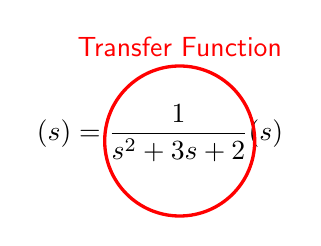
\begin{tikzpicture}
\draw (0,0) node {$\displaystyle\outptLT(s) = \frac{1}{s^{2}+3s+2}\inptLT(s)$};
\visible<6->{\draw (0.25,-.1) node[circle,draw,color=red,minimum width=.75in,very thick] {};
\draw (.25,1.1) node[color=red] {\textsf{Transfer Function}};}
\end{tikzpicture}
\end{center}
}
\end{frame}
}

In terms of our input and output signal and system block/arrow representation, we can visualize this example in the Laplace domain as
\begin{frame}
	\begin{center}
		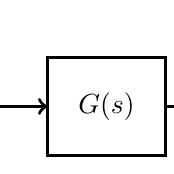
\begin{tikzpicture}[inner sep=0pt,outer sep=0pt,very thick,
sysblock/.style={draw,rectangle,inner sep=2pt,minimum width=1.5cm,minimum height=1.25cm,very thick}]
\useasboundingbox (-1,1) rectangle (0.5,-0.5); 
\begin{scope}[transform canvas={scale=1}]
\draw (0,0) node[sysblock] (S) {$G(s)$};
\draw[->] (-2,0) node[above=2pt] {$R(s)$} -- (S.180);
\draw[->] (S.0) -- ++(1.5,0) node[above=2pt] {$Y(s)$};
\end{scope}
\end{tikzpicture}

	\end{center}
\end{frame}
\noindent where $R(s)$ is the Laplace transform of the input signal, $Y(s)$ is the Laplace transform of the output signal, and the transfer function $G(s)  = \frac{1}{s^2 + 3s + 2}$ represents the system we are modeling. This diagram is an example of a \textit{block diagram}, which we will formalize in the upcoming Lecture~\BlockDiagramsNumber.

\begin{frame}{Transfer function definition}
\begin{definition}
The {\em Transfer Function} ($G(s)$) of a (linear, time invariant) system is the ratio of the Laplace Transform of the output signal over the Laplace Transform of the input signal with zero initial conditions.
\end{definition}
\mode<presentation>{\[
\visible<2->{\frac{\outptLT(s)}{\inptLT(s)} = \plant(s)} \quad \quad \visible<3->{\outptLT(s)= \plant(s)\inptLT(s)}
\]}
\end{frame}

For the system described by the example differential equation above, the transfer function, $\plant(s)$ is
\[
\plant(s) = \frac{\outptLT(s)}{\inptLT(s)} = \frac{1}{s^{2}+3s+2}.
\]
Given the transfer function, and a system input $\inpt(t)$, we need only find the Laplace Transform, $\inptLT(s)$, and multiply it by $\plant(s)$ to get the Laplace Transform of the output, i.e.
\[
 \outptLT(s)= \plant(s)\inptLT(s).
\]
As we will see, the ability to use multiplication (algebra) instead of integration (calculus) to predict behavior of a system is one advantage of using transfer functions instead of differential equations in control systems. 

\mode<presentation>{
\begin{frame}{Finding the Transfer Function}
\begin{itemize}[<+->]
\item Current Method:
\begin{itemize}
\item Write down all the (differential) equations describing the system
\item Eliminate all variables except input and output
\item Find the Laplace Transform of the resulting differential equation
\end{itemize}
\item Impedance Method:
\begin{itemize}
\item Write down all the (differential) equations describing the system
\item Take the Laplace Transform of these equations
\item Eliminate all variables except input and output
\end{itemize}
\end{itemize}

\end{frame}
}

\section{Finding Transfer Functions Using Impedance
\label{sec:findingTFs}}

One way to find a transfer function is to first find the differential equation describing the system, transform the equation to the Laplace domain, then solve for the output using Laplace Transform techniques. However, rather than first using algebra to find a differential equation and then using Laplace Transforms, it is also possible to do the reverse: find the Laplace Transform of all components, and then use our algebraic rules to solve for the transfer function. This is best explained using examples. 

We will start by looking at electrical systems. We have the following component laws:

\begin{frame}{Electrical Components}
\begin{center}
\begin{tabular}{c|ccc}
 & resistor & capacitor & inductor \\\hline
\rule{0pt}{14pt} Component law & $v=iR$ & $C\frac{dv}{dt} = i$ & $v=L\frac{di}{dt}$ \\
\rule{0pt}{14pt} Laplace Transform & \visible<2->{$V(s)= RI(s)$} & \visible<3->{$CsV(s) = I(s)$} & \visible<4->{$V(s) = LsI(s)$}
 \end{tabular}
\end{center}
\end{frame}

Once in the Laplace domain, the relationship between current and voltage is algebraic for all elements. The ratio between the voltage and current for a particular element defines the behavior of that element.

\begin{frame}
\begin{definition}
The {\em impedance} of an element is the ratio of the Laplace Transform of the across variable (voltage) over the Laplace Transform of the through variable (current)
\end{definition}
\end{frame}{}
A common point of confusion arises from the fact that the ``block'' depiction of an impedance element looks similar to the block depiction of a system in a block diagram such as shown in Section~\ref{sec:TFs}. However, the two are not equivalent. In this lecture, we demonstrate the use of the impedance blocks to model system elements so they can be solved using circuit analysis concepts. 

\mode<article>{\begin{frame}{Electrical Impedance}
\begin{center}
\begin{tabular}{c|ccc}
 & resistor & capacitor & inductor \\\hline
\rule{0pt}{14pt} Impedance & $\frac{V(s)}{I(s)}=R$ & $\frac{V(s)}{I(s)} = \frac{1}{sC}$ & $\frac{V(s)}{I(s)} = Ls$ \\
 \end{tabular}
\end{center}
\end{frame}}

\mode<presentation>{\begin{frame}{Electrical Impedance}
\begin{center}
\begin{tabular}{c|ccc}
 & resistor & capacitor & inductor \\\hline
 \rule{0pt}{14pt} Component law & $v=iR$ & $C\frac{dv}{dt} = i$ & $v=L\frac{di}{dt}$ \\
\rule{0pt}{14pt} Laplace Transform & $V(s)= RI(s)$ & $CsV(s) = I(s)$ & $V(s) = LsI(s)$\\
\rule{0pt}{14pt} Impedance & $\frac{V(s)}{I(s)}=R$ & $\frac{V(s)}{I(s)} = \frac{1}{sC}$ & $\frac{V(s)}{I(s)} = Ls$ \\
 \end{tabular}
\end{center}
\end{frame}}


\mode<presentation>{\begin{frame}
\begin{center}
\input{figures/seriescircuit}
\end{center}
\end{frame}}

\mode<presentation>{\begin{frame}{Impedance Circuit}
\begin{center}
\begin{tikzpicture}[scale=1.5,inner sep=0pt,outer sep=0pt,very thick]
\draw (0,0) node (a) {}; 
\draw (4,0) node (c) {};
\draw (0,-2) node (d) {};
\draw (4,-2) node (f) {};
 
\draw (1,0) node (R1) {\documentclass[12pt]{article}
% \newcommand{\mainfolder}{/Users/coulston/Dropbox/EENG307Current}  	                    % @ Work PC
%\newcommand{\mainfolder}{C:/Users/Chris/Dropbox/Mycourses/EENG307Current}  	% @ Work Laptop
\newcommand{\mainfolder}{C:/Users/chris/Dropbox/Mycourses/EENG307Current}		% @ Home PC

% \newcommand{\mainfolder}{$HOME/Dropbox/EENG307Current}
\newcommand{\commonmaterial}{\mainfolder/CommonMaterial}
\input{\mainfolder/Headers/packageheader}
\input{\mainfolder/Headers/coursedefheader}

\usepackage{pbox}
%\usepackage{siunitx}
%\usepackage{draftwatermark}
%\SetWatermarkText{DRAFT}
%\SetWatermarkScale{1}

\setlength{\topmargin}{-.75in}
\setlength{\textheight}{9.25in}
\setlength{\oddsidemargin}{-0.25in}
\setlength{\evensidemargin}{-0.25in}
\setlength{\textwidth}{7in}




\begin{document}



%%%%%%%%%%%%%%%%%%%%%%%%%%%%%%%%%%%
\begin{frame}{Electrical Impedance}%
\begin{center}%
\mode<article>{

\begin{tabular}{c|ccc}
 & resistor & capacitor & inductor  \\\hline
 Component & \input{./figures/resistor.tex} & \input{./figures/capacitor.tex} & \input{./figures/inductor.tex}\\\hline
\rule[-8pt]{0pt}{0pt}\rule{0pt}{14pt} 
Component law & $v_1-v_2=iR$ & $i = C\frac{d(v_1-v_2)}{dt}$ & $v_1-v_2=L\frac{di}{dt}$  \\\hline
\rule[-8pt]{0pt}{0pt}\rule{0pt}{14pt} 
Laplace Transform & $V(s)= I(s)R$ & $V(s) = \frac{1}{Cs}I(s)$ & $V(s) = LsI(s)$ \\\hline
Impedance Component & \input{./figures/resistorimpedance.tex} & \input{./figures/capacitorimpedance.tex} & \input{./figures/inductorimpedance.tex}

\end{tabular}}
\end{center}
\end{frame}


%%%%%%%%%%%%%%%%%%%%%%%%%%%%%%%%%%%
\begin{frame}{Fluid Impedance}
\graphicspath{}
\begin{center}
\mode<article>{

\begin{tabular}{c|cc}
 & valve & tank \\\hline
%Component &\begin{tikzpicture}
\draw (.75,0) node (valve) {\input{\mainfolder/DrawingElements/FluidElements/valve.tex}};
\draw (.75,0) node[above=9pt] {$R$};
\draw (-.2,.25) node[above] {$p_{1}$};
\draw[<-] (valve.180) --  ++(-.5,0) node[left] {$q$};
\draw[->] (valve.0) -- ++(.5,0)  node[right] {$q$};
\draw (1.7,.25) node[above] {$p_{2}$};
\draw (.75,1.5) node {$p = p_{1}-p_{2}$};
\end{tikzpicture} &  \input{./figures/figurestank2.tex} \\\hline
Component &\begin{tikzpicture}
\draw (.75,0) node (valve) {\input{\mainfolder/DrawingElements/FluidElements/valve.tex}};
\draw (.75,0) node[above=9pt] {$R$};
\draw (-.2,.25) node[above] {$p_{1}$};
\draw[<-] (valve.180) --  ++(-.5,0) node[left] {$q$};
\draw[->] (valve.0) -- ++(.5,0)  node[right] {$q$};
\draw (1.7,.25) node[above] {$p_{2}$};
\draw (.75,1.5) node {$p = p_{1}-p_{2}$};
\end{tikzpicture} &  \input{./figures/tank.tex} \\\hline
\rule[-8pt]{0pt}{0pt}\rule{0pt}{14pt} Component law & $p=Rq$ & $\frac{A}{\rho g}\frac{dp}{dt} = q_{1} - q_{2}$ \\\hline
\rule[-8pt]{0pt}{0pt}\rule{0pt}{14pt} Laplace Transform & $P(s)= RQ(s)$ & $\frac{A}{\rho g}sP(s) = Q_{1}(s)-Q_{2}(s)$ \\\hline
 Impedance Component & \input{./figures/valveanalogycopy.tex} & \input{./figures/tankanalogycopy.tex}
 \end{tabular}}
 
\mode<presentation>{\resizebox{11cm}{!}{

\begin{tabular}{c|cc}
 & valve & tank \\\hline
Component &\begin{tikzpicture}
\draw (.75,0) node (valve) {\input{\mainfolder/DrawingElements/FluidElements/valve.tex}};
\draw (.75,0) node[above=9pt] {$R$};
\draw (-.2,.25) node[above] {$p_{1}$};
\draw[<-] (valve.180) --  ++(-.5,0) node[left] {$q$};
\draw[->] (valve.0) -- ++(.5,0)  node[right] {$q$};
\draw (1.7,.25) node[above] {$p_{2}$};
\draw (.75,1.5) node {$p = p_{1}-p_{2}$};
\end{tikzpicture} & \input{./figures/tank2.tex} \\\hline
\rule[-8pt]{0pt}{0pt}\rule{0pt}{14pt} Component law & $p=Rq$ & $\frac{A}{\rho g}\frac{dp}{dt} = q_{1} - q_{2}$ \\\hline
\rule[-8pt]{0pt}{0pt}\rule{0pt}{14pt} Laplace Transform & $P(s)= RQ(s)$ & $\frac{A}{\rho g}sP(s) = Q_{1}(s)-Q_{2}(s)$ \\\hline
 Impedance Component & \input{./figures/valveanalogycopy.tex} & \input{./figures/tankanalogycopy.tex}
 \end{tabular}}}
\end{center}
\end{frame}

\pagebreak

%%%%%%%%%%%%%%%%%%%%%%%%%%%%%%%%%%%
\begin{frame}{Mechanical Impedance}%
\begin{center}%
\mode<article>{\begin{tabular}{c|ccc}
 & mass & spring & damper \\\hline
 Component & \begin{tikzpicture}
%  \draw(-1,2.5) node (text) {\textsf{fixed point}};
%   \draw[->] (text.180) -- ++(-.7,0);
   \draw[inner sep=0pt,outer sep=0pt,very thick] (-3,1) node (gnd1) {\input{\mainfolder/DrawingElements/MechanicalElements/ground.tex}};
   \draw[->|,dotted] (-3,1.75) -- node[pos=.5,above] {$x_{f}$} ++(3.6,0); 
    \draw[very thick] (0,0) rectangle (1.2,1);
    \draw (.6,.5) node {$m$};
    \draw[->,thick] (1.2,.5) -- ++(.5,0) node[right] {$f$};
    \draw[|->,thick] (.6,1.2) node[above=2pt] {$x$} -- ++(.5,0);  
\end{tikzpicture}
 & \begin{tikzpicture}
\draw (.75,0) node[inner sep=0,outer sep=0] (K1) {\input{\mainfolder/DrawingElements/MechanicalElements/spring.tex}};
\draw (K1)  node[above=6pt] {$k$};
\draw[very thick] (K1.180) -- ++(-.2,0);
\draw[very thick] (K1.0) -- ++(0.2,0);
\draw[<-,thick] (K1.0) ++(.2,0) -- ++(.5,0) node[right] {$f$};
\draw[<-,thick] (K1.180) ++(-.2,0) -- ++(-.5,0) node[left] {$f$};
\draw[|->,thick] (K1.180) ++(-.2,.4) node[above=2pt] {$x_{1}$} -- ++(.5,0);  
\draw[|->,thick] (K1.0) ++(.2,.4) node[above=2pt] {$x_{2}$} -- ++(.5,0);  
\draw<2-> (K1) ++(0,-.6) node {$f=k(x_{1}-x_{2})$};
\end{tikzpicture}
 & \begin{tikzpicture}
\draw[very thick] (-.2,0) -- (0,0);
\draw (.75,0) node {\input{\mainfolder/DrawingElements/MechanicalElements/damper.tex}};
\draw (.75,0) node[above=9pt] {$b$};
\draw[very thick] (1.5,0) -- ++(.2,0);
    \draw[<-,thick] (1.5,0) ++(.2,0) -- ++(.5,0) node[right] {$f$};
    \draw[<-,thick] (-.2,0) -- ++(-.5,0) node[left] {$f$};
    \draw[|->,thick] (-.2,.4) node[above=2pt] {$x_{1}$} -- ++(.5,0);  
    \draw[|->,thick] (1.7,.4) node[above=2pt] {$x_{2}$} -- ++(.5,0);  
    \draw (.6,-.6) node {$x=x_{1}-x_{2}$};
  %  \draw (.6,-1.2) node {$f=b\dot{x}$};
\end{tikzpicture}\\\hline
\rule[-8pt]{0pt}{0pt}\rule{0pt}{14pt} 
Component law & $f = m\ddot{x}$ & $f = kx$ & $f=b\dot{x}$  \\\hline
\rule[-8pt]{0pt}{0pt}\rule{0pt}{14pt} Laplace Transform & $X(s)= \frac{1}{ms^{2}}F(s)$ & $X(s) = \frac{1}{k}F(s)$ & $X(s) = \frac{1}{bs}F(s)$ \\\hline
\begin{minipage}[b]{1.5in}\begin{center}Impedance Component \\
(positive $f$ direction agrees with positive $x$ direction)\end{center}
\end{minipage}
& \input{figures/massimpedance.tex} & \input{figures/springimpedance.tex} & \input{figures/damperimpedance.tex}
 \end{tabular}}
\mode<presentation>{\resizebox{10cm}{!}{\begin{tabular}{c|ccc}
 & mass & spring & damper \\\hline
 Component & \begin{tikzpicture}
%  \draw(-1,2.5) node (text) {\textsf{fixed point}};
%   \draw[->] (text.180) -- ++(-.7,0);
   \draw[inner sep=0pt,outer sep=0pt,very thick] (-3,1) node (gnd1) {\input{\mainfolder/DrawingElements/MechanicalElements/ground.tex}};
   \draw[->|,dotted] (-3,1.75) -- node[pos=.5,above] {$x_{f}$} ++(3.6,0); 
    \draw[very thick] (0,0) rectangle (1.2,1);
    \draw (.6,.5) node {$m$};
    \draw[->,thick] (1.2,.5) -- ++(.5,0) node[right] {$f$};
    \draw[|->,thick] (.6,1.2) node[above=2pt] {$x$} -- ++(.5,0);  
\end{tikzpicture}
& \begin{tikzpicture}
\draw (.75,0) node[inner sep=0,outer sep=0] (K1) {\input{\mainfolder/DrawingElements/MechanicalElements/spring.tex}};
\draw (K1)  node[above=6pt] {$k$};
\draw[very thick] (K1.180) -- ++(-.2,0);
\draw[very thick] (K1.0) -- ++(0.2,0);
\draw[<-,thick] (K1.0) ++(.2,0) -- ++(.5,0) node[right] {$f$};
\draw[<-,thick] (K1.180) ++(-.2,0) -- ++(-.5,0) node[left] {$f$};
\draw[|->,thick] (K1.180) ++(-.2,.4) node[above=2pt] {$x_{1}$} -- ++(.5,0);  
\draw[|->,thick] (K1.0) ++(.2,.4) node[above=2pt] {$x_{2}$} -- ++(.5,0);  
\draw<2-> (K1) ++(0,-.6) node {$f=k(x_{1}-x_{2})$};
\end{tikzpicture}
 & \begin{tikzpicture}
\draw[very thick] (-.2,0) -- (0,0);
\draw (.75,0) node {\input{\mainfolder/DrawingElements/MechanicalElements/damper.tex}};
\draw (.75,0) node[above=9pt] {$b$};
\draw[very thick] (1.5,0) -- ++(.2,0);
    \draw[<-,thick] (1.5,0) ++(.2,0) -- ++(.5,0) node[right] {$f$};
    \draw[<-,thick] (-.2,0) -- ++(-.5,0) node[left] {$f$};
    \draw[|->,thick] (-.2,.4) node[above=2pt] {$x_{1}$} -- ++(.5,0);  
    \draw[|->,thick] (1.7,.4) node[above=2pt] {$x_{2}$} -- ++(.5,0);  
    \draw (.6,-.6) node {$x=x_{1}-x_{2}$};
  %  \draw (.6,-1.2) node {$f=b\dot{x}$};
\end{tikzpicture}\\\hline
\rule{0pt}{14pt} Component law & $M\ddot{x}=f$ & $f = kx$ & $f=b\dot{x}$  \\\hline
\rule[-8pt]{0pt}{0pt}\rule{0pt}{14pt} Laplace Transform & $X(s)= \frac{1}{Ms^{2}}F(s)$ & $X(s) = \frac{1}{k}F(s)$ & $X(s) = \frac{1}{bs}F(s)$ \\\hline
\begin{minipage}[b]{1.5in}\begin{center}Impedance Component \\
(positive $f$ direction agrees with positive $x$ direction)\end{center}
\end{minipage}
& \input{./figures/massimpedance.tex} & \input{./figures/springimpedance.tex} & \input{./figures/damperimpedance.tex}
 \end{tabular}}}
\end{center}
\end{frame}


%%%%%%%%%%%%%%%%%%%%%%%%%%%%%%%%%%%
\begin{frame}{Rotational Impedance}
\begin{center}
\mode<article>{\begin{tabular}{c|ccc}
 & mass & spring & damper \\\hline
 Component & \begin{minipage}[b]{.75in}\begin{tikzpicture}
    \draw[very thick] (.5,0) node[cylinder,draw,shape aspect=.55,minimum width=1cm,minimum height=1.5cm] (J) {$J$};
    \draw[->] (-.2,.5) node[above] {$\theta$}  .. controls  ++(-.15,-.3) and ++(-.15,.3) ..  ++(0,-1);
    \draw[->] (1.4,-.5) node[below] {$\tau$}  .. controls  ++(.15,.3) and ++(.15,-.3) ..  ++(0,1);
    \draw (.5,-1) node {$J\ddot{\theta}=\tau$};
\end{tikzpicture}\\\vspace{.1in}\end{minipage} & \begin{tikzpicture}
\draw[very thick] (-.2,0) -- (0,0);
\draw (.75,0) node {\input{\mainfolder/DrawingElements/MechanicalElements/spring.tex}};
\draw[very  thick] (1.5,0) -- ++(.2,0);
\draw (.75,0) node[above=9pt] {$k$};
\draw[->] (-.2,.5) node[above] {$\theta_{1}$}  .. controls  ++(-.15,-.3) and ++(-.15,.3) ..  ++(0,-1);
\draw[->] (-.5,.5) node[above] {$\tau$}  .. controls  ++(-.15,-.3) and ++(-.15,.3) ..  ++(0,-1);
\draw[->] (1.5,.5) node[above] {$\theta_{2}$}  .. controls  ++(-.15,-.3) and ++(-.15,.3) ..  ++(0,-1);
\draw[->] (1.9,.5) node[above] {$\tau$}  .. controls  ++(.15,-.3) and ++(.15,.3) ..  ++(0,-1);
\draw (.5,-1) node {$\theta=\theta_{1} - \theta_{2}$};
\end{tikzpicture} & \begin{tikzpicture}
\draw[very thick] (-.2,0) -- (0,0);
\draw (.75,0) node {\input{\mainfolder/DrawingElements/MechanicalElements/damper.tex}};
\draw[very  thick] (1.5,0) -- ++(.2,0);
\draw (.75,0) node[above=9pt] {$b$};
\draw[->] (-.2,.5) node[above] {$\theta_{1}$}  .. controls  ++(-.15,-.3) and ++(-.15,.3) ..  ++(0,-1);
\draw[->] (-.5,.5) node[above] {$\tau$}  .. controls  ++(-.15,-.3) and ++(-.15,.3) ..  ++(0,-1);
\draw[->] (1.5,.5) node[above] {$\theta_{2}$}  .. controls  ++(-.15,-.3) and ++(-.15,.3) ..  ++(0,-1);
\draw[->] (1.9,.5) node[above] {$\tau$}  .. controls  ++(.15,-.3) and ++(.15,.3) ..  ++(0,-1);
\draw (.5,-1) node {$\dot{\theta}=\dot{\theta}_{1} - \dot{\theta}_{2}$};
\end{tikzpicture}\\\hline
 \rule[-8pt]{0pt}{0pt}\rule{0pt}{12pt} 
 Component Law & $\tau = J\ddot{\theta}$ & $\tau = k\theta$ & $\tau = b\dot{\theta}$ \\\hline
\rule[-8pt]{0pt}{0pt}\rule{0pt}{14pt} Laplace Transform & $\theta(s)= \frac{1}{Js^{2}}\tau(s)$ & $\theta(s) = \frac{1}{k}\tau(s)$ & $\theta(s) = \frac{1}{bs}\tau(s)$ \\\hline
\begin{minipage}[b]{1.5in}\begin{center}Impedance Component
\end{center}
\end{minipage}
& \begin{tikzpicture}
\draw (0,0) node (R) {\begin{tikzpicture}
\draw (0,0) node[circle,fill,inner sep=1pt,] {} node[above] {$\theta$};
\draw[very thick] (0,0)  -- ++(0,-.37);
\draw[very thick] (0,-1) node[rectangle,draw,minimum width=.1in,minimum height=.5in] {};
\draw[very thick] (0,-1.65) -- ++(0,-.37);
\draw[very thick] (0,-2) node{\input{\mainfolder/DrawingElements/CircuitElements/elground.tex}};
\end{tikzpicture}
};

\draw (R) node[right=6pt] {$\frac{1}{Js^{2}}$};
%\draw (6.1,.75) node[above] {$+$};
\draw (1,0) node[right] {$\begin{matrix} + \\ \\ \theta(s)\\  \\ - \end{matrix}$};
%\draw (7.9,.75) node[above] {$-$};
\draw[->] (-.3,.5) -- node[pos=.5,left] {$\tau(s)$} ++(0,-1);  

\end{tikzpicture} & \begin{tikzpicture}
\draw (7,.2) node (R) {\begin{tikzpicture}
\draw (0,0) node[circle,fill,inner sep=1pt,] {} node[above] {$\theta_{1}$};
\draw[very thick] (0,0) -- ++(.37,0);
\draw[very thick] (1,0) node[rectangle,draw,minimum width=.5in,minimum height=.1in] {};
\draw[very thick] (1.65,0) -- ++(.37,0);
\draw (2.02,0) node[circle,fill,inner sep=1pt,] {} node[above] {$\theta_{2}$};
\end{tikzpicture}
};
\draw (R) node[above=1pt] {$\frac{1}{k}$};
%\draw (6.1,.75) node[above] {$+$};
%\draw (7,.75) node[above] {$X(s)$};
%\draw (7.9,.75) node[above] {$-$};
\draw[->] (6.5,-.3) -- node[pos=.5,below] {$\tau(s)$} ++(1,0);  
\draw (7,-1.5) node[above] {$\begin{matrix} + & \theta(s) & - \end{matrix}$};

\end{tikzpicture} & \input{./figures/rotdamperimpedance.tex}
 \end{tabular}}
\mode<presentation>{\resizebox{10cm}{!}{\begin{tabular}{c|ccc}
 & mass & spring & damper \\\hline
 Component & \begin{tikzpicture}
    \draw[very thick] (.5,0) node[cylinder,draw,shape aspect=.55,minimum width=1cm,minimum height=1.5cm] (J) {$J$};
    \draw[->] (-.2,.5) node[above] {$\theta$}  .. controls  ++(-.15,-.3) and ++(-.15,.3) ..  ++(0,-1);
    \draw[->] (1.4,-.5) node[below] {$\tau$}  .. controls  ++(.15,.3) and ++(.15,-.3) ..  ++(0,1);
    \draw (.5,-1) node {$J\ddot{\theta}=\tau$};
\end{tikzpicture} & \begin{tikzpicture}
\draw[very thick] (-.2,0) -- (0,0);
\draw (.75,0) node {\input{\mainfolder/DrawingElements/MechanicalElements/spring.tex}};
\draw[very  thick] (1.5,0) -- ++(.2,0);
\draw (.75,0) node[above=9pt] {$k$};
\draw[->] (-.2,.5) node[above] {$\theta_{1}$}  .. controls  ++(-.15,-.3) and ++(-.15,.3) ..  ++(0,-1);
\draw[->] (-.5,.5) node[above] {$\tau$}  .. controls  ++(-.15,-.3) and ++(-.15,.3) ..  ++(0,-1);
\draw[->] (1.5,.5) node[above] {$\theta_{2}$}  .. controls  ++(-.15,-.3) and ++(-.15,.3) ..  ++(0,-1);
\draw[->] (1.9,.5) node[above] {$\tau$}  .. controls  ++(.15,-.3) and ++(.15,.3) ..  ++(0,-1);
\draw (.5,-1) node {$\theta=\theta_{1} - \theta_{2}$};
\end{tikzpicture} & \begin{tikzpicture}
\draw[very thick] (-.2,0) -- (0,0);
\draw (.75,0) node {\input{\mainfolder/DrawingElements/MechanicalElements/damper.tex}};
\draw[very  thick] (1.5,0) -- ++(.2,0);
\draw (.75,0) node[above=9pt] {$b$};
\draw[->] (-.2,.5) node[above] {$\theta_{1}$}  .. controls  ++(-.15,-.3) and ++(-.15,.3) ..  ++(0,-1);
\draw[->] (-.5,.5) node[above] {$\tau$}  .. controls  ++(-.15,-.3) and ++(-.15,.3) ..  ++(0,-1);
\draw[->] (1.5,.5) node[above] {$\theta_{2}$}  .. controls  ++(-.15,-.3) and ++(-.15,.3) ..  ++(0,-1);
\draw[->] (1.9,.5) node[above] {$\tau$}  .. controls  ++(.15,-.3) and ++(.15,.3) ..  ++(0,-1);
\draw (.5,-1) node {$\dot{\theta}=\dot{\theta}_{1} - \dot{\theta}_{2}$};
\end{tikzpicture}\\\hline
\rule[-8pt]{0pt}{0pt}\rule{0pt}{14pt} Laplace Transform & $\theta(s)= \frac{1}{Js^{2}}\tau(s)$ & $\theta(s) = \frac{1}{k}\tau(s)$ & $\theta(s) = \frac{1}{bs}\tau(s)$ \\\hline
\begin{minipage}[b]{1.5in}\begin{center}Impedance Component 
\end{center}
\end{minipage}
& \begin{tikzpicture}
\draw (0,0) node (R) {\begin{tikzpicture}
\draw (0,0) node[circle,fill,inner sep=1pt,] {} node[above] {$\theta$};
\draw[very thick] (0,0)  -- ++(0,-.37);
\draw[very thick] (0,-1) node[rectangle,draw,minimum width=.1in,minimum height=.5in] {};
\draw[very thick] (0,-1.65) -- ++(0,-.37);
\draw[very thick] (0,-2) node{\input{\mainfolder/DrawingElements/CircuitElements/elground.tex}};
\end{tikzpicture}
};

\draw (R) node[right=6pt] {$\frac{1}{Js^{2}}$};
%\draw (6.1,.75) node[above] {$+$};
\draw (1,0) node[right] {$\begin{matrix} + \\ \\ \theta(s)\\  \\ - \end{matrix}$};
%\draw (7.9,.75) node[above] {$-$};
\draw[->] (-.3,.5) -- node[pos=.5,left] {$\tau(s)$} ++(0,-1);  

\end{tikzpicture} & \begin{tikzpicture}
\draw (7,.2) node (R) {\begin{tikzpicture}
\draw (0,0) node[circle,fill,inner sep=1pt,] {} node[above] {$\theta_{1}$};
\draw[very thick] (0,0) -- ++(.37,0);
\draw[very thick] (1,0) node[rectangle,draw,minimum width=.5in,minimum height=.1in] {};
\draw[very thick] (1.65,0) -- ++(.37,0);
\draw (2.02,0) node[circle,fill,inner sep=1pt,] {} node[above] {$\theta_{2}$};
\end{tikzpicture}
};
\draw (R) node[above=1pt] {$\frac{1}{k}$};
%\draw (6.1,.75) node[above] {$+$};
%\draw (7,.75) node[above] {$X(s)$};
%\draw (7.9,.75) node[above] {$-$};
\draw[->] (6.5,-.3) -- node[pos=.5,below] {$\tau(s)$} ++(1,0);  
\draw (7,-1.5) node[above] {$\begin{matrix} + & \theta(s) & - \end{matrix}$};

\end{tikzpicture} & \input{./figures/rotdamperimpedance.tex}
 \end{tabular}}}
\end{center}
\end{frame}


\pagebreak

%%%%%%%%%%%%%%%%%%%%%%%%%%%%%%%%%%%
\begin{frame}{Thermal Impedance}
\begin{center}
\begin{tabular}{c|ccc}
 & Resistance & Capacitance & Convection \\\hline
 
 
Component & 
%-------- Thermal Resistance :''Brick wall''
\begin{tikzpicture}
\draw[pattern=bricks]  (0,-2) -- ++(0,4) -- ++(.25,0) -- ++(0,-4)  -- cycle;
\draw (-1,1) node {$T_{1}$};
\draw (1,1) node {$T_{2}$};
\draw[->] (-.5,0) -- ++(1,0) node[right=2pt] {$\dot{Q}$}; 
\end{tikzpicture}
 & 
 %--------- Thermal Capacitance ''Heat Chamber''
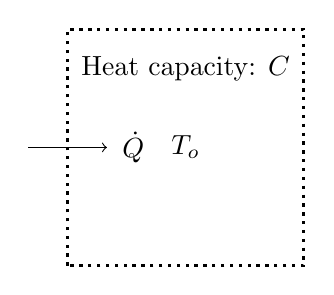
\begin{tikzpicture}
\draw[dotted,very thick]  (-1.5,-1.5) rectangle (1.5,1.5);
\draw (0,0) node {$T_{o}$};
\draw (0,1) node {Heat capacity: $C$};
\draw[->] (-2,0) -- ++(1,0) node[right=2pt] {$\dot{Q}$}; 
\end{tikzpicture} 
& 
%--------- Thermal Convection ''Heat Flow''
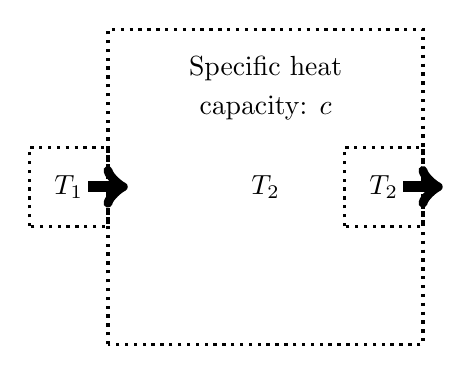
\begin{tikzpicture}
\draw[dotted,very thick]  (-2,-2) rectangle (2,2);
\draw[dotted,very thick]  (-3,-0.5) rectangle ++(1,1);
\draw[dotted,very thick]  (1,-0.5) rectangle ++(1,1);
\draw (0,1.5) node {Specific heat};
\draw (0,1.0) node {capacity: $c$};
\draw (0,0) node {$T_{2}$};
\draw (-2.5,0) node {$T_{1}$};
\draw (1.5,0) node {$T_{2}$};
\draw[->,line width=4pt] (-2.25,0) -- ++(.5,0);
\draw[->,line width=4pt] (1.75,0) -- ++(.5,0);
 \end{tikzpicture}  
 \\\hline

\rule[-8pt]{0pt}{0pt}\rule{0pt}{14pt}  
Component law & 		$T = \dot{Q}R$ & 
							$\dot{Q} = C \frac{dT_o}{dt}$ & 
							$\dot{Q} = \dot{m} c T$ \\\hline
							
\rule[-8pt]{0pt}{0pt}\rule{0pt}{14pt}							
Laplace Transform &	$T(s)=\dot{Q}(s)R$ & 
							$\dot{Q}(s)=CsT_o(s)$ & 
							$\dot{Q}(s)=\dot{m}cT(s)$ \\\hline

 							 
Impedance Component  &  
 %--------- Thermal resistance model
 \begin{tikzpicture}
\draw (5,0) node[inner sep=0,outer sep=0] (C) {\input{../DrawingElements/CircuitElements/resistor.tex}};
\draw (C) node[above=12pt] {$R$};
\draw[->] (C.0) ++(.1,0) -- node[pos=.5,below=2pt] {$\dot{Q}$} ++(.5,0);
\draw[<-] (C.180) ++(-.1,0) -- node[pos=.5,below=2pt] {$\dot{Q}$} ++(-.5,0);
\draw (C.0) node[draw,fill,inner sep=0pt,outer sep=0pt,circle] {$\rule{2pt}{0pt}$};
\draw (C.0) node[above=4pt] {$T_{2}$};
\draw (C.180) node[draw,fill,inner sep=0pt,outer sep=0pt,circle] {$\rule{2pt}{0pt}$};
\draw (C.180) node[above=4pt] {$T_{1}$};
%\draw (C) ++(0,-1) node {$\dot{Q}R = T_{1} - T_{2}$};
\draw (C) ++(0,-1) node {$T = T_{1} - T_{2}$};
\end{tikzpicture} 
& 
%--------- Thermal capacitor model
 \begin{tikzpicture} 
\draw (5,0) node[inner sep=0,outer sep=0,rotate=90] (C) {\input{../DrawingElements/CircuitElements/capacitor.tex}};
\draw (C) node[right=12pt] {$\frac{1}{Cs}$};
\draw[->] (C.0) ++(.3,0) -- node[pos=0,right=2pt] {$\dot{Q}$} ++(0,-.5);
\draw (C.0) node[draw,fill,inner sep=0pt,outer sep=0pt,circle] {$\rule{2pt}{0pt}$};
\draw (C.0) node[above=4pt] {$T_{o}$};
\draw (C.180) node[draw,fill,inner sep=0pt,outer sep=0pt,circle] {$\rule{2pt}{0pt}$};
\draw (C.180) node[below=4pt] {$T_{ref}=0$}; 
\end{tikzpicture} 
& 
 \begin{tikzpicture} 
\draw (7,0) node (C) {\input{../DrawingElements/CircuitElements/resistor.tex}};
\draw (5,0) node[isosceles triangle,draw,very thick,inner sep=2pt] (G) {$1$};
\draw (C) node[above=12pt] {$R=\frac{1}{c\dot{m}}$};
\draw[very thick] (G.180) ++(-.75,0) node[draw,fill,inner sep=0pt,outer sep=0pt,circle] (Gin) {$\rule{2pt}{0pt}$} -- (G.180);
\draw (Gin) node[above=4pt] {$T_{1}$};
\draw[<-] (Gin) ++(-.1,0) -- node[pos=-1.5,below left=2pt] {$\dot{Q}_{in}=0$} ++(-.5,0);
\draw[very thick] (G.0) ++(-0.1,0) --   ++(0.8,0) ;
\draw[very thick] (C.0) ++(-0.2,0) -- ++(.5,0) node (C_p) {} node[above=4pt]  {$T_{2}$};
\draw (C_p.0)++(-0.1,0) node[draw,fill,inner sep=0pt,outer sep=0pt,circle] {$\rule{2pt}{0pt}$};
\draw[->] (C_p.0) ++(.1,0) -- node[pos=-.5,below right=2pt] {$\dot{Q}$} ++(.5,0);
\draw (C) ++(0,-1) node {$T = T_{1} - T_{2}$};
\end{tikzpicture}

\end{tabular}
\end{center}
\end{frame}


%%%%%%%%%%%%%%%%%%%%%%%%%%%%%%%%%%%
\begin{frame}{DC Motor}
\begin{center}
\begin{tabular}{c|c}
   &   DC motor \\\hline
   
Component & 
\begin{tikzpicture}[scale=1.3,inner sep=0pt,outer sep=0pt,very thick]
\draw (0,0) node[fill=black] (a) {}; 
\draw (3.5,0) node[fill=black] (c) {};
\draw (0,-2) node[fill=black] (d) {};
\draw (2,-2) node[fill=black] (e) {};
\draw (3.5,-2) node[fill=black] (f) {};
 
\draw (1,0) node (R1) {\input{../DrawingElements/CircuitElements/resistor.tex}};
\draw (1,0) node[above=.2in] {$R_{a}$};
\draw (2.5,0) node (L1) {\input{../DrawingElements/CircuitElements/inductor.tex}};
\draw (2.5,0) node[above=.2in] {$L_{a}$};
\draw (3.5,-1) node (Rot) {\input{../DrawingElements/CircuitElements/rotor.tex}}; 
\draw[->] (4,-1) ++(0,.5)  node[above=2pt] {$\theta$}  .. controls  ++(-.15,-.3) and ++(-.15,.3) ..  ++(0,-1);
\draw[->] (4.25,-1) ++(0,.5) node[above=2pt] {$\tau_{m}$}  .. controls  ++(-.15,-.3) and ++(-.15,.3) ..  ++(0,-1);
\draw[->] (3.35,-.1) -- node[left=1pt] {$i_{a}$} ++(0,-.5); 
\draw (3.5,-1) node[left=.2in] {$\begin{matrix} + \\ v_{b} \\ -\end{matrix}$};
\draw (0,-1) node (V) {\input{../DrawingElements/CircuitElements/voltagesource.tex}};
\draw (0,-1) node[left=.2in]{$v_{a}$};
\draw (a) -- (R1);
\draw (R1) -- (L1);
\draw (L1) -| (Rot);
\draw (Rot) -- (f);
\draw (f) -- (d);
\draw (a) -- (V);
\draw (d) -- (V);


\end{tikzpicture}
 \\\hline
 
 						 
Component Law &  	
\pbox{10cm}
{$v_{b} = K_{e}\dot{\theta}$ \\ 
$\tau_{m} = K_{t} i_{a}$ \\ 
$v_a(t) = i_a(t)R + L\frac{di_a(t)}{dt} + v_b(t)$ }

\\\hline
 							 
Block Diagram  &  
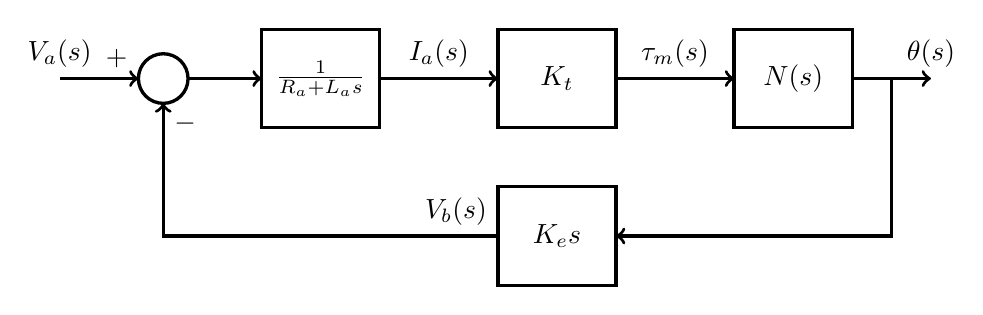
\begin{tikzpicture}[inner sep=0pt,outer sep=0pt,very thick,
sysblock/.style={draw,rectangle,inner sep=2pt,minimum width=1.5cm,minimum height=1.25cm,very thick}]
\draw (0,0) node[draw,circle] (sum) {$\rule{0pt}{18pt}$};
\draw (2,0) node[sysblock] (a) {$\frac{1}{R_{a} + L_{a}s}$};
\draw (5,0) node[sysblock] (b) {$K_{t}$};
\draw (8,0) node[sysblock] (c) {$N(s)$};
\draw (5,-2) node[sysblock] (d) {$K_{e}s$};
\draw[<-] (sum.180) node[above left=4pt] {$+$} -- ++(-1,0) node[above=4pt] {$V_{a}(s)$};
\draw[->] (sum.0) -- (a.180);
\draw[->] (a.0) -- node[pos=.5,above=4pt] {$I_{a}(s)$} (b.180);
\draw[->] (b.0) -- node[pos=.5,above=4pt] {$\tau_{m}(s)$} (c.180);
\draw[->] (c.0) -- ++(1,0) node[above=4pt] {$\theta(s)$};
\draw[->] (c.0) -- ++(.5,0) |- (d.0);
\draw[->] (d.180) node[above left=4pt] {$V_{b}(s)$} -| (sum.-90) node[below right=4pt] {$-$};
\end{tikzpicture}  
\end{tabular}
\end{center}
\end{frame}


%%%%%%%%%%%%%%%%%%%%%%%%%%%%%%%%%%%
\pagebreak
\begin{frame}{Hydraulic}
\begin{center}
\begin{tabular}{c|c}
   &   Hydraulic \\\hline

Component &    
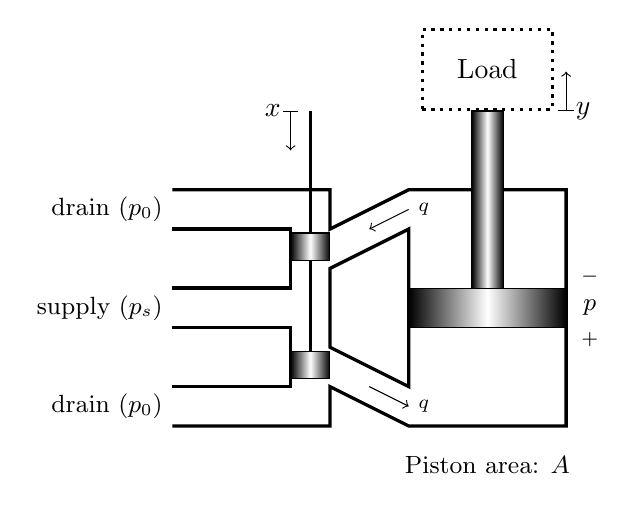
\begin{tikzpicture}
% tank
\draw[very thick] (0,0) -- ++(2,0) -- ++(0,-.5) -- ++(1,.5) -- ++(2,0) -- ++(0,-3) -- ++(-2,0) -- ++(-1,.5) -- ++(0,-.5) -- ++(-2,0);
\draw[very thick] (0,-.5) -- ++(1.5,0) -- ++(0,-.75) -- ++(-1.5,0);
\draw[very thick] (0,-1.75) -- ++(1.5,0) -- ++(0,-.75) -- ++(-1.5,0);
\draw[very thick] (2,-1) -- ++(1,.5) -- ++(0,-2) -- ++(-1,.5) -- cycle;
\draw (4,-3.5) node {\small Piston area: $A$};
\draw (0,-.25) node[left] {\small drain ($p_{0}$)};
\draw (0,-1.5) node[left] {\small supply ($p_{s}$)};
\draw (0,-2.75) node[left] {\small drain ($p_{0}$)};
\draw[->] (3,-.25) node[right] {\scriptsize$q$} -- ++(-.5,-.25);
\draw[->] (2.5,-2.5) -- ++(.5,-.25)  node[right] {\scriptsize$q$};
\draw (5.3,-1.9) node {\scriptsize $+$} ++(0,.4) node{\small $p$} ++(0,.4) node {\scriptsize$-$};

% valves
\draw[very thick,color=black] (1.75,-2.1) -- ++(0,3.1);
\draw[fill,left color=black,right color=black,middle color=white] (1.5,-.9) rectangle ++(.5,.35);
\draw[fill,left color=black,right color=black,middle color=white] (1.5,-2.4) rectangle ++(.5,.35);
\draw[|->] (1.5,1) node[left] {$x$} -- ++(0,-.5); 

% piston
\draw[fill,left color=black,right color=black,middle color=white] (4,-1.5) ++(-.2,0) rectangle ++(.4,2.5);
\draw[fill,left color=black,right color=black,middle color=white] (3,-1.75) rectangle ++(2,.5);
\draw[|->] (5,1) node[right] {$y$} -- ++(0,.5);

% load
\draw (4,1) node[draw,very thick,above,dotted,rectangle,minimum width=.65in,minimum height=.4in] {Load};
\end{tikzpicture}
\\\hline

\rule[-8pt]{0pt}{0pt}
Component Law &  
\pbox{10cm}
{$\delta q = k_x\delta x - k_p \delta p$ \\
$f = p A $ \\
$y = \frac{1}{A} \int q dt $ }

\\\hline

Block Diagram & 
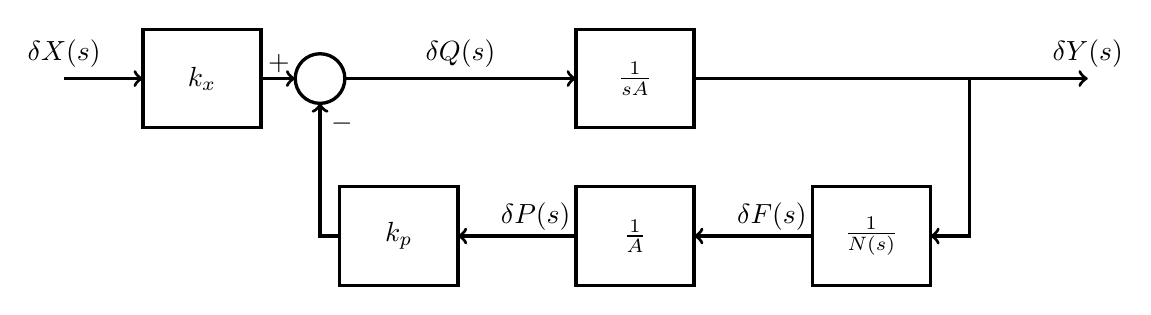
\begin{tikzpicture}[inner sep=0pt,outer sep=0pt,very thick,
sysblock/.style={draw,rectangle,inner sep=2pt,minimum width=1.5cm,minimum height=1.25cm,very thick}]
\draw (-1.5,0) node[sysblock] (d) {$k_{x}$};
\draw (0,0) node[draw,circle] (sum) {$\rule{0pt}{18pt}$};
\draw (4,0) node[sysblock] (a) {$\frac{1}{sA}$};
\draw (4,-2) node[sysblock] (b) {$\frac{1}{A}$};
\draw (7,-2) node[sysblock] (b1) {$\frac{1}{N(s)}$};
\draw (1,-2) node[sysblock] (c) {$k_{p}$};
\draw[<-] (d.180)  -- ++(-1,0) node[above=4pt] {$\delta X(s)$};
\draw[->] (d.0) -- (sum.180) node[above left=2pt] {$+$};
\draw[->] (sum.0) -- node[pos=.5,above=4pt] {$\delta Q(s)$} (a.180);
\draw[->] (a.0) -- ++(5,0) node[above=4pt] {$\delta Y(s)$};
\draw[->] (a.0) -- ++(3.5,0) |- (b1.0);
\draw[->] (b1.180) node[above left=2pt] {$\delta F(s)$} -- (b.0);
\draw[->] (b.180) node[above left=2pt] {$\delta P(s)$} -- (c.0);
\draw[->] (c.180)  -| (sum.-90) node[below right=4pt] {$-$};

\end{tikzpicture}





\end{tabular}
\end{center}
\end{frame}

\end{document}


};
\draw (1,0) node[above=.2in] {$R$};
\draw (3,0) node (L1) {\documentclass[12pt]{article}
% \newcommand{\mainfolder}{/Users/coulston/Dropbox/EENG307Current}  	                    % @ Work PC
%\newcommand{\mainfolder}{C:/Users/Chris/Dropbox/Mycourses/EENG307Current}  	% @ Work Laptop
\newcommand{\mainfolder}{C:/Users/chris/Dropbox/Mycourses/EENG307Current}		% @ Home PC

% \newcommand{\mainfolder}{$HOME/Dropbox/EENG307Current}
\newcommand{\commonmaterial}{\mainfolder/CommonMaterial}
\input{\mainfolder/Headers/packageheader}
\input{\mainfolder/Headers/coursedefheader}

\usepackage{pbox}
%\usepackage{siunitx}
%\usepackage{draftwatermark}
%\SetWatermarkText{DRAFT}
%\SetWatermarkScale{1}

\setlength{\topmargin}{-.75in}
\setlength{\textheight}{9.25in}
\setlength{\oddsidemargin}{-0.25in}
\setlength{\evensidemargin}{-0.25in}
\setlength{\textwidth}{7in}




\begin{document}



%%%%%%%%%%%%%%%%%%%%%%%%%%%%%%%%%%%
\begin{frame}{Electrical Impedance}%
\begin{center}%
\mode<article>{

\begin{tabular}{c|ccc}
 & resistor & capacitor & inductor  \\\hline
 Component & \input{./figures/resistor.tex} & \input{./figures/capacitor.tex} & \input{./figures/inductor.tex}\\\hline
\rule[-8pt]{0pt}{0pt}\rule{0pt}{14pt} 
Component law & $v_1-v_2=iR$ & $i = C\frac{d(v_1-v_2)}{dt}$ & $v_1-v_2=L\frac{di}{dt}$  \\\hline
\rule[-8pt]{0pt}{0pt}\rule{0pt}{14pt} 
Laplace Transform & $V(s)= I(s)R$ & $V(s) = \frac{1}{Cs}I(s)$ & $V(s) = LsI(s)$ \\\hline
Impedance Component & \input{./figures/resistorimpedance.tex} & \input{./figures/capacitorimpedance.tex} & \input{./figures/inductorimpedance.tex}

\end{tabular}}
\end{center}
\end{frame}


%%%%%%%%%%%%%%%%%%%%%%%%%%%%%%%%%%%
\begin{frame}{Fluid Impedance}
\graphicspath{}
\begin{center}
\mode<article>{

\begin{tabular}{c|cc}
 & valve & tank \\\hline
%Component &\begin{tikzpicture}
\draw (.75,0) node (valve) {\input{\mainfolder/DrawingElements/FluidElements/valve.tex}};
\draw (.75,0) node[above=9pt] {$R$};
\draw (-.2,.25) node[above] {$p_{1}$};
\draw[<-] (valve.180) --  ++(-.5,0) node[left] {$q$};
\draw[->] (valve.0) -- ++(.5,0)  node[right] {$q$};
\draw (1.7,.25) node[above] {$p_{2}$};
\draw (.75,1.5) node {$p = p_{1}-p_{2}$};
\end{tikzpicture} &  \input{./figures/figurestank2.tex} \\\hline
Component &\begin{tikzpicture}
\draw (.75,0) node (valve) {\input{\mainfolder/DrawingElements/FluidElements/valve.tex}};
\draw (.75,0) node[above=9pt] {$R$};
\draw (-.2,.25) node[above] {$p_{1}$};
\draw[<-] (valve.180) --  ++(-.5,0) node[left] {$q$};
\draw[->] (valve.0) -- ++(.5,0)  node[right] {$q$};
\draw (1.7,.25) node[above] {$p_{2}$};
\draw (.75,1.5) node {$p = p_{1}-p_{2}$};
\end{tikzpicture} &  \input{./figures/tank.tex} \\\hline
\rule[-8pt]{0pt}{0pt}\rule{0pt}{14pt} Component law & $p=Rq$ & $\frac{A}{\rho g}\frac{dp}{dt} = q_{1} - q_{2}$ \\\hline
\rule[-8pt]{0pt}{0pt}\rule{0pt}{14pt} Laplace Transform & $P(s)= RQ(s)$ & $\frac{A}{\rho g}sP(s) = Q_{1}(s)-Q_{2}(s)$ \\\hline
 Impedance Component & \input{./figures/valveanalogycopy.tex} & \input{./figures/tankanalogycopy.tex}
 \end{tabular}}
 
\mode<presentation>{\resizebox{11cm}{!}{

\begin{tabular}{c|cc}
 & valve & tank \\\hline
Component &\begin{tikzpicture}
\draw (.75,0) node (valve) {\input{\mainfolder/DrawingElements/FluidElements/valve.tex}};
\draw (.75,0) node[above=9pt] {$R$};
\draw (-.2,.25) node[above] {$p_{1}$};
\draw[<-] (valve.180) --  ++(-.5,0) node[left] {$q$};
\draw[->] (valve.0) -- ++(.5,0)  node[right] {$q$};
\draw (1.7,.25) node[above] {$p_{2}$};
\draw (.75,1.5) node {$p = p_{1}-p_{2}$};
\end{tikzpicture} & \input{./figures/tank2.tex} \\\hline
\rule[-8pt]{0pt}{0pt}\rule{0pt}{14pt} Component law & $p=Rq$ & $\frac{A}{\rho g}\frac{dp}{dt} = q_{1} - q_{2}$ \\\hline
\rule[-8pt]{0pt}{0pt}\rule{0pt}{14pt} Laplace Transform & $P(s)= RQ(s)$ & $\frac{A}{\rho g}sP(s) = Q_{1}(s)-Q_{2}(s)$ \\\hline
 Impedance Component & \input{./figures/valveanalogycopy.tex} & \input{./figures/tankanalogycopy.tex}
 \end{tabular}}}
\end{center}
\end{frame}

\pagebreak

%%%%%%%%%%%%%%%%%%%%%%%%%%%%%%%%%%%
\begin{frame}{Mechanical Impedance}%
\begin{center}%
\mode<article>{\begin{tabular}{c|ccc}
 & mass & spring & damper \\\hline
 Component & \begin{tikzpicture}
%  \draw(-1,2.5) node (text) {\textsf{fixed point}};
%   \draw[->] (text.180) -- ++(-.7,0);
   \draw[inner sep=0pt,outer sep=0pt,very thick] (-3,1) node (gnd1) {\input{\mainfolder/DrawingElements/MechanicalElements/ground.tex}};
   \draw[->|,dotted] (-3,1.75) -- node[pos=.5,above] {$x_{f}$} ++(3.6,0); 
    \draw[very thick] (0,0) rectangle (1.2,1);
    \draw (.6,.5) node {$m$};
    \draw[->,thick] (1.2,.5) -- ++(.5,0) node[right] {$f$};
    \draw[|->,thick] (.6,1.2) node[above=2pt] {$x$} -- ++(.5,0);  
\end{tikzpicture}
 & \begin{tikzpicture}
\draw (.75,0) node[inner sep=0,outer sep=0] (K1) {\input{\mainfolder/DrawingElements/MechanicalElements/spring.tex}};
\draw (K1)  node[above=6pt] {$k$};
\draw[very thick] (K1.180) -- ++(-.2,0);
\draw[very thick] (K1.0) -- ++(0.2,0);
\draw[<-,thick] (K1.0) ++(.2,0) -- ++(.5,0) node[right] {$f$};
\draw[<-,thick] (K1.180) ++(-.2,0) -- ++(-.5,0) node[left] {$f$};
\draw[|->,thick] (K1.180) ++(-.2,.4) node[above=2pt] {$x_{1}$} -- ++(.5,0);  
\draw[|->,thick] (K1.0) ++(.2,.4) node[above=2pt] {$x_{2}$} -- ++(.5,0);  
\draw<2-> (K1) ++(0,-.6) node {$f=k(x_{1}-x_{2})$};
\end{tikzpicture}
 & \begin{tikzpicture}
\draw[very thick] (-.2,0) -- (0,0);
\draw (.75,0) node {\input{\mainfolder/DrawingElements/MechanicalElements/damper.tex}};
\draw (.75,0) node[above=9pt] {$b$};
\draw[very thick] (1.5,0) -- ++(.2,0);
    \draw[<-,thick] (1.5,0) ++(.2,0) -- ++(.5,0) node[right] {$f$};
    \draw[<-,thick] (-.2,0) -- ++(-.5,0) node[left] {$f$};
    \draw[|->,thick] (-.2,.4) node[above=2pt] {$x_{1}$} -- ++(.5,0);  
    \draw[|->,thick] (1.7,.4) node[above=2pt] {$x_{2}$} -- ++(.5,0);  
    \draw (.6,-.6) node {$x=x_{1}-x_{2}$};
  %  \draw (.6,-1.2) node {$f=b\dot{x}$};
\end{tikzpicture}\\\hline
\rule[-8pt]{0pt}{0pt}\rule{0pt}{14pt} 
Component law & $f = m\ddot{x}$ & $f = kx$ & $f=b\dot{x}$  \\\hline
\rule[-8pt]{0pt}{0pt}\rule{0pt}{14pt} Laplace Transform & $X(s)= \frac{1}{ms^{2}}F(s)$ & $X(s) = \frac{1}{k}F(s)$ & $X(s) = \frac{1}{bs}F(s)$ \\\hline
\begin{minipage}[b]{1.5in}\begin{center}Impedance Component \\
(positive $f$ direction agrees with positive $x$ direction)\end{center}
\end{minipage}
& \input{figures/massimpedance.tex} & \input{figures/springimpedance.tex} & \input{figures/damperimpedance.tex}
 \end{tabular}}
\mode<presentation>{\resizebox{10cm}{!}{\begin{tabular}{c|ccc}
 & mass & spring & damper \\\hline
 Component & \begin{tikzpicture}
%  \draw(-1,2.5) node (text) {\textsf{fixed point}};
%   \draw[->] (text.180) -- ++(-.7,0);
   \draw[inner sep=0pt,outer sep=0pt,very thick] (-3,1) node (gnd1) {\input{\mainfolder/DrawingElements/MechanicalElements/ground.tex}};
   \draw[->|,dotted] (-3,1.75) -- node[pos=.5,above] {$x_{f}$} ++(3.6,0); 
    \draw[very thick] (0,0) rectangle (1.2,1);
    \draw (.6,.5) node {$m$};
    \draw[->,thick] (1.2,.5) -- ++(.5,0) node[right] {$f$};
    \draw[|->,thick] (.6,1.2) node[above=2pt] {$x$} -- ++(.5,0);  
\end{tikzpicture}
& \begin{tikzpicture}
\draw (.75,0) node[inner sep=0,outer sep=0] (K1) {\input{\mainfolder/DrawingElements/MechanicalElements/spring.tex}};
\draw (K1)  node[above=6pt] {$k$};
\draw[very thick] (K1.180) -- ++(-.2,0);
\draw[very thick] (K1.0) -- ++(0.2,0);
\draw[<-,thick] (K1.0) ++(.2,0) -- ++(.5,0) node[right] {$f$};
\draw[<-,thick] (K1.180) ++(-.2,0) -- ++(-.5,0) node[left] {$f$};
\draw[|->,thick] (K1.180) ++(-.2,.4) node[above=2pt] {$x_{1}$} -- ++(.5,0);  
\draw[|->,thick] (K1.0) ++(.2,.4) node[above=2pt] {$x_{2}$} -- ++(.5,0);  
\draw<2-> (K1) ++(0,-.6) node {$f=k(x_{1}-x_{2})$};
\end{tikzpicture}
 & \begin{tikzpicture}
\draw[very thick] (-.2,0) -- (0,0);
\draw (.75,0) node {\input{\mainfolder/DrawingElements/MechanicalElements/damper.tex}};
\draw (.75,0) node[above=9pt] {$b$};
\draw[very thick] (1.5,0) -- ++(.2,0);
    \draw[<-,thick] (1.5,0) ++(.2,0) -- ++(.5,0) node[right] {$f$};
    \draw[<-,thick] (-.2,0) -- ++(-.5,0) node[left] {$f$};
    \draw[|->,thick] (-.2,.4) node[above=2pt] {$x_{1}$} -- ++(.5,0);  
    \draw[|->,thick] (1.7,.4) node[above=2pt] {$x_{2}$} -- ++(.5,0);  
    \draw (.6,-.6) node {$x=x_{1}-x_{2}$};
  %  \draw (.6,-1.2) node {$f=b\dot{x}$};
\end{tikzpicture}\\\hline
\rule{0pt}{14pt} Component law & $M\ddot{x}=f$ & $f = kx$ & $f=b\dot{x}$  \\\hline
\rule[-8pt]{0pt}{0pt}\rule{0pt}{14pt} Laplace Transform & $X(s)= \frac{1}{Ms^{2}}F(s)$ & $X(s) = \frac{1}{k}F(s)$ & $X(s) = \frac{1}{bs}F(s)$ \\\hline
\begin{minipage}[b]{1.5in}\begin{center}Impedance Component \\
(positive $f$ direction agrees with positive $x$ direction)\end{center}
\end{minipage}
& \input{./figures/massimpedance.tex} & \input{./figures/springimpedance.tex} & \input{./figures/damperimpedance.tex}
 \end{tabular}}}
\end{center}
\end{frame}


%%%%%%%%%%%%%%%%%%%%%%%%%%%%%%%%%%%
\begin{frame}{Rotational Impedance}
\begin{center}
\mode<article>{\begin{tabular}{c|ccc}
 & mass & spring & damper \\\hline
 Component & \begin{minipage}[b]{.75in}\begin{tikzpicture}
    \draw[very thick] (.5,0) node[cylinder,draw,shape aspect=.55,minimum width=1cm,minimum height=1.5cm] (J) {$J$};
    \draw[->] (-.2,.5) node[above] {$\theta$}  .. controls  ++(-.15,-.3) and ++(-.15,.3) ..  ++(0,-1);
    \draw[->] (1.4,-.5) node[below] {$\tau$}  .. controls  ++(.15,.3) and ++(.15,-.3) ..  ++(0,1);
    \draw (.5,-1) node {$J\ddot{\theta}=\tau$};
\end{tikzpicture}\\\vspace{.1in}\end{minipage} & \begin{tikzpicture}
\draw[very thick] (-.2,0) -- (0,0);
\draw (.75,0) node {\input{\mainfolder/DrawingElements/MechanicalElements/spring.tex}};
\draw[very  thick] (1.5,0) -- ++(.2,0);
\draw (.75,0) node[above=9pt] {$k$};
\draw[->] (-.2,.5) node[above] {$\theta_{1}$}  .. controls  ++(-.15,-.3) and ++(-.15,.3) ..  ++(0,-1);
\draw[->] (-.5,.5) node[above] {$\tau$}  .. controls  ++(-.15,-.3) and ++(-.15,.3) ..  ++(0,-1);
\draw[->] (1.5,.5) node[above] {$\theta_{2}$}  .. controls  ++(-.15,-.3) and ++(-.15,.3) ..  ++(0,-1);
\draw[->] (1.9,.5) node[above] {$\tau$}  .. controls  ++(.15,-.3) and ++(.15,.3) ..  ++(0,-1);
\draw (.5,-1) node {$\theta=\theta_{1} - \theta_{2}$};
\end{tikzpicture} & \begin{tikzpicture}
\draw[very thick] (-.2,0) -- (0,0);
\draw (.75,0) node {\input{\mainfolder/DrawingElements/MechanicalElements/damper.tex}};
\draw[very  thick] (1.5,0) -- ++(.2,0);
\draw (.75,0) node[above=9pt] {$b$};
\draw[->] (-.2,.5) node[above] {$\theta_{1}$}  .. controls  ++(-.15,-.3) and ++(-.15,.3) ..  ++(0,-1);
\draw[->] (-.5,.5) node[above] {$\tau$}  .. controls  ++(-.15,-.3) and ++(-.15,.3) ..  ++(0,-1);
\draw[->] (1.5,.5) node[above] {$\theta_{2}$}  .. controls  ++(-.15,-.3) and ++(-.15,.3) ..  ++(0,-1);
\draw[->] (1.9,.5) node[above] {$\tau$}  .. controls  ++(.15,-.3) and ++(.15,.3) ..  ++(0,-1);
\draw (.5,-1) node {$\dot{\theta}=\dot{\theta}_{1} - \dot{\theta}_{2}$};
\end{tikzpicture}\\\hline
 \rule[-8pt]{0pt}{0pt}\rule{0pt}{12pt} 
 Component Law & $\tau = J\ddot{\theta}$ & $\tau = k\theta$ & $\tau = b\dot{\theta}$ \\\hline
\rule[-8pt]{0pt}{0pt}\rule{0pt}{14pt} Laplace Transform & $\theta(s)= \frac{1}{Js^{2}}\tau(s)$ & $\theta(s) = \frac{1}{k}\tau(s)$ & $\theta(s) = \frac{1}{bs}\tau(s)$ \\\hline
\begin{minipage}[b]{1.5in}\begin{center}Impedance Component
\end{center}
\end{minipage}
& \begin{tikzpicture}
\draw (0,0) node (R) {\begin{tikzpicture}
\draw (0,0) node[circle,fill,inner sep=1pt,] {} node[above] {$\theta$};
\draw[very thick] (0,0)  -- ++(0,-.37);
\draw[very thick] (0,-1) node[rectangle,draw,minimum width=.1in,minimum height=.5in] {};
\draw[very thick] (0,-1.65) -- ++(0,-.37);
\draw[very thick] (0,-2) node{\input{\mainfolder/DrawingElements/CircuitElements/elground.tex}};
\end{tikzpicture}
};

\draw (R) node[right=6pt] {$\frac{1}{Js^{2}}$};
%\draw (6.1,.75) node[above] {$+$};
\draw (1,0) node[right] {$\begin{matrix} + \\ \\ \theta(s)\\  \\ - \end{matrix}$};
%\draw (7.9,.75) node[above] {$-$};
\draw[->] (-.3,.5) -- node[pos=.5,left] {$\tau(s)$} ++(0,-1);  

\end{tikzpicture} & \begin{tikzpicture}
\draw (7,.2) node (R) {\begin{tikzpicture}
\draw (0,0) node[circle,fill,inner sep=1pt,] {} node[above] {$\theta_{1}$};
\draw[very thick] (0,0) -- ++(.37,0);
\draw[very thick] (1,0) node[rectangle,draw,minimum width=.5in,minimum height=.1in] {};
\draw[very thick] (1.65,0) -- ++(.37,0);
\draw (2.02,0) node[circle,fill,inner sep=1pt,] {} node[above] {$\theta_{2}$};
\end{tikzpicture}
};
\draw (R) node[above=1pt] {$\frac{1}{k}$};
%\draw (6.1,.75) node[above] {$+$};
%\draw (7,.75) node[above] {$X(s)$};
%\draw (7.9,.75) node[above] {$-$};
\draw[->] (6.5,-.3) -- node[pos=.5,below] {$\tau(s)$} ++(1,0);  
\draw (7,-1.5) node[above] {$\begin{matrix} + & \theta(s) & - \end{matrix}$};

\end{tikzpicture} & \input{./figures/rotdamperimpedance.tex}
 \end{tabular}}
\mode<presentation>{\resizebox{10cm}{!}{\begin{tabular}{c|ccc}
 & mass & spring & damper \\\hline
 Component & \begin{tikzpicture}
    \draw[very thick] (.5,0) node[cylinder,draw,shape aspect=.55,minimum width=1cm,minimum height=1.5cm] (J) {$J$};
    \draw[->] (-.2,.5) node[above] {$\theta$}  .. controls  ++(-.15,-.3) and ++(-.15,.3) ..  ++(0,-1);
    \draw[->] (1.4,-.5) node[below] {$\tau$}  .. controls  ++(.15,.3) and ++(.15,-.3) ..  ++(0,1);
    \draw (.5,-1) node {$J\ddot{\theta}=\tau$};
\end{tikzpicture} & \begin{tikzpicture}
\draw[very thick] (-.2,0) -- (0,0);
\draw (.75,0) node {\input{\mainfolder/DrawingElements/MechanicalElements/spring.tex}};
\draw[very  thick] (1.5,0) -- ++(.2,0);
\draw (.75,0) node[above=9pt] {$k$};
\draw[->] (-.2,.5) node[above] {$\theta_{1}$}  .. controls  ++(-.15,-.3) and ++(-.15,.3) ..  ++(0,-1);
\draw[->] (-.5,.5) node[above] {$\tau$}  .. controls  ++(-.15,-.3) and ++(-.15,.3) ..  ++(0,-1);
\draw[->] (1.5,.5) node[above] {$\theta_{2}$}  .. controls  ++(-.15,-.3) and ++(-.15,.3) ..  ++(0,-1);
\draw[->] (1.9,.5) node[above] {$\tau$}  .. controls  ++(.15,-.3) and ++(.15,.3) ..  ++(0,-1);
\draw (.5,-1) node {$\theta=\theta_{1} - \theta_{2}$};
\end{tikzpicture} & \begin{tikzpicture}
\draw[very thick] (-.2,0) -- (0,0);
\draw (.75,0) node {\input{\mainfolder/DrawingElements/MechanicalElements/damper.tex}};
\draw[very  thick] (1.5,0) -- ++(.2,0);
\draw (.75,0) node[above=9pt] {$b$};
\draw[->] (-.2,.5) node[above] {$\theta_{1}$}  .. controls  ++(-.15,-.3) and ++(-.15,.3) ..  ++(0,-1);
\draw[->] (-.5,.5) node[above] {$\tau$}  .. controls  ++(-.15,-.3) and ++(-.15,.3) ..  ++(0,-1);
\draw[->] (1.5,.5) node[above] {$\theta_{2}$}  .. controls  ++(-.15,-.3) and ++(-.15,.3) ..  ++(0,-1);
\draw[->] (1.9,.5) node[above] {$\tau$}  .. controls  ++(.15,-.3) and ++(.15,.3) ..  ++(0,-1);
\draw (.5,-1) node {$\dot{\theta}=\dot{\theta}_{1} - \dot{\theta}_{2}$};
\end{tikzpicture}\\\hline
\rule[-8pt]{0pt}{0pt}\rule{0pt}{14pt} Laplace Transform & $\theta(s)= \frac{1}{Js^{2}}\tau(s)$ & $\theta(s) = \frac{1}{k}\tau(s)$ & $\theta(s) = \frac{1}{bs}\tau(s)$ \\\hline
\begin{minipage}[b]{1.5in}\begin{center}Impedance Component 
\end{center}
\end{minipage}
& \begin{tikzpicture}
\draw (0,0) node (R) {\begin{tikzpicture}
\draw (0,0) node[circle,fill,inner sep=1pt,] {} node[above] {$\theta$};
\draw[very thick] (0,0)  -- ++(0,-.37);
\draw[very thick] (0,-1) node[rectangle,draw,minimum width=.1in,minimum height=.5in] {};
\draw[very thick] (0,-1.65) -- ++(0,-.37);
\draw[very thick] (0,-2) node{\input{\mainfolder/DrawingElements/CircuitElements/elground.tex}};
\end{tikzpicture}
};

\draw (R) node[right=6pt] {$\frac{1}{Js^{2}}$};
%\draw (6.1,.75) node[above] {$+$};
\draw (1,0) node[right] {$\begin{matrix} + \\ \\ \theta(s)\\  \\ - \end{matrix}$};
%\draw (7.9,.75) node[above] {$-$};
\draw[->] (-.3,.5) -- node[pos=.5,left] {$\tau(s)$} ++(0,-1);  

\end{tikzpicture} & \begin{tikzpicture}
\draw (7,.2) node (R) {\begin{tikzpicture}
\draw (0,0) node[circle,fill,inner sep=1pt,] {} node[above] {$\theta_{1}$};
\draw[very thick] (0,0) -- ++(.37,0);
\draw[very thick] (1,0) node[rectangle,draw,minimum width=.5in,minimum height=.1in] {};
\draw[very thick] (1.65,0) -- ++(.37,0);
\draw (2.02,0) node[circle,fill,inner sep=1pt,] {} node[above] {$\theta_{2}$};
\end{tikzpicture}
};
\draw (R) node[above=1pt] {$\frac{1}{k}$};
%\draw (6.1,.75) node[above] {$+$};
%\draw (7,.75) node[above] {$X(s)$};
%\draw (7.9,.75) node[above] {$-$};
\draw[->] (6.5,-.3) -- node[pos=.5,below] {$\tau(s)$} ++(1,0);  
\draw (7,-1.5) node[above] {$\begin{matrix} + & \theta(s) & - \end{matrix}$};

\end{tikzpicture} & \input{./figures/rotdamperimpedance.tex}
 \end{tabular}}}
\end{center}
\end{frame}


\pagebreak

%%%%%%%%%%%%%%%%%%%%%%%%%%%%%%%%%%%
\begin{frame}{Thermal Impedance}
\begin{center}
\begin{tabular}{c|ccc}
 & Resistance & Capacitance & Convection \\\hline
 
 
Component & 
%-------- Thermal Resistance :''Brick wall''
\begin{tikzpicture}
\draw[pattern=bricks]  (0,-2) -- ++(0,4) -- ++(.25,0) -- ++(0,-4)  -- cycle;
\draw (-1,1) node {$T_{1}$};
\draw (1,1) node {$T_{2}$};
\draw[->] (-.5,0) -- ++(1,0) node[right=2pt] {$\dot{Q}$}; 
\end{tikzpicture}
 & 
 %--------- Thermal Capacitance ''Heat Chamber''
\begin{tikzpicture}
\draw[dotted,very thick]  (-1.5,-1.5) rectangle (1.5,1.5);
\draw (0,0) node {$T_{o}$};
\draw (0,1) node {Heat capacity: $C$};
\draw[->] (-2,0) -- ++(1,0) node[right=2pt] {$\dot{Q}$}; 
\end{tikzpicture} 
& 
%--------- Thermal Convection ''Heat Flow''
\begin{tikzpicture}
\draw[dotted,very thick]  (-2,-2) rectangle (2,2);
\draw[dotted,very thick]  (-3,-0.5) rectangle ++(1,1);
\draw[dotted,very thick]  (1,-0.5) rectangle ++(1,1);
\draw (0,1.5) node {Specific heat};
\draw (0,1.0) node {capacity: $c$};
\draw (0,0) node {$T_{2}$};
\draw (-2.5,0) node {$T_{1}$};
\draw (1.5,0) node {$T_{2}$};
\draw[->,line width=4pt] (-2.25,0) -- ++(.5,0);
\draw[->,line width=4pt] (1.75,0) -- ++(.5,0);
 \end{tikzpicture}  
 \\\hline

\rule[-8pt]{0pt}{0pt}\rule{0pt}{14pt}  
Component law & 		$T = \dot{Q}R$ & 
							$\dot{Q} = C \frac{dT_o}{dt}$ & 
							$\dot{Q} = \dot{m} c T$ \\\hline
							
\rule[-8pt]{0pt}{0pt}\rule{0pt}{14pt}							
Laplace Transform &	$T(s)=\dot{Q}(s)R$ & 
							$\dot{Q}(s)=CsT_o(s)$ & 
							$\dot{Q}(s)=\dot{m}cT(s)$ \\\hline

 							 
Impedance Component  &  
 %--------- Thermal resistance model
 \begin{tikzpicture}
\draw (5,0) node[inner sep=0,outer sep=0] (C) {\input{../DrawingElements/CircuitElements/resistor.tex}};
\draw (C) node[above=12pt] {$R$};
\draw[->] (C.0) ++(.1,0) -- node[pos=.5,below=2pt] {$\dot{Q}$} ++(.5,0);
\draw[<-] (C.180) ++(-.1,0) -- node[pos=.5,below=2pt] {$\dot{Q}$} ++(-.5,0);
\draw (C.0) node[draw,fill,inner sep=0pt,outer sep=0pt,circle] {$\rule{2pt}{0pt}$};
\draw (C.0) node[above=4pt] {$T_{2}$};
\draw (C.180) node[draw,fill,inner sep=0pt,outer sep=0pt,circle] {$\rule{2pt}{0pt}$};
\draw (C.180) node[above=4pt] {$T_{1}$};
%\draw (C) ++(0,-1) node {$\dot{Q}R = T_{1} - T_{2}$};
\draw (C) ++(0,-1) node {$T = T_{1} - T_{2}$};
\end{tikzpicture} 
& 
%--------- Thermal capacitor model
 \begin{tikzpicture} 
\draw (5,0) node[inner sep=0,outer sep=0,rotate=90] (C) {\input{../DrawingElements/CircuitElements/capacitor.tex}};
\draw (C) node[right=12pt] {$\frac{1}{Cs}$};
\draw[->] (C.0) ++(.3,0) -- node[pos=0,right=2pt] {$\dot{Q}$} ++(0,-.5);
\draw (C.0) node[draw,fill,inner sep=0pt,outer sep=0pt,circle] {$\rule{2pt}{0pt}$};
\draw (C.0) node[above=4pt] {$T_{o}$};
\draw (C.180) node[draw,fill,inner sep=0pt,outer sep=0pt,circle] {$\rule{2pt}{0pt}$};
\draw (C.180) node[below=4pt] {$T_{ref}=0$}; 
\end{tikzpicture} 
& 
 \begin{tikzpicture} 
\draw (7,0) node (C) {\input{../DrawingElements/CircuitElements/resistor.tex}};
\draw (5,0) node[isosceles triangle,draw,very thick,inner sep=2pt] (G) {$1$};
\draw (C) node[above=12pt] {$R=\frac{1}{c\dot{m}}$};
\draw[very thick] (G.180) ++(-.75,0) node[draw,fill,inner sep=0pt,outer sep=0pt,circle] (Gin) {$\rule{2pt}{0pt}$} -- (G.180);
\draw (Gin) node[above=4pt] {$T_{1}$};
\draw[<-] (Gin) ++(-.1,0) -- node[pos=-1.5,below left=2pt] {$\dot{Q}_{in}=0$} ++(-.5,0);
\draw[very thick] (G.0) ++(-0.1,0) --   ++(0.8,0) ;
\draw[very thick] (C.0) ++(-0.2,0) -- ++(.5,0) node (C_p) {} node[above=4pt]  {$T_{2}$};
\draw (C_p.0)++(-0.1,0) node[draw,fill,inner sep=0pt,outer sep=0pt,circle] {$\rule{2pt}{0pt}$};
\draw[->] (C_p.0) ++(.1,0) -- node[pos=-.5,below right=2pt] {$\dot{Q}$} ++(.5,0);
\draw (C) ++(0,-1) node {$T = T_{1} - T_{2}$};
\end{tikzpicture}

\end{tabular}
\end{center}
\end{frame}


%%%%%%%%%%%%%%%%%%%%%%%%%%%%%%%%%%%
\begin{frame}{DC Motor}
\begin{center}
\begin{tabular}{c|c}
   &   DC motor \\\hline
   
Component & 
\begin{tikzpicture}[scale=1.3,inner sep=0pt,outer sep=0pt,very thick]
\draw (0,0) node[fill=black] (a) {}; 
\draw (3.5,0) node[fill=black] (c) {};
\draw (0,-2) node[fill=black] (d) {};
\draw (2,-2) node[fill=black] (e) {};
\draw (3.5,-2) node[fill=black] (f) {};
 
\draw (1,0) node (R1) {\input{../DrawingElements/CircuitElements/resistor.tex}};
\draw (1,0) node[above=.2in] {$R_{a}$};
\draw (2.5,0) node (L1) {\input{../DrawingElements/CircuitElements/inductor.tex}};
\draw (2.5,0) node[above=.2in] {$L_{a}$};
\draw (3.5,-1) node (Rot) {\input{../DrawingElements/CircuitElements/rotor.tex}}; 
\draw[->] (4,-1) ++(0,.5)  node[above=2pt] {$\theta$}  .. controls  ++(-.15,-.3) and ++(-.15,.3) ..  ++(0,-1);
\draw[->] (4.25,-1) ++(0,.5) node[above=2pt] {$\tau_{m}$}  .. controls  ++(-.15,-.3) and ++(-.15,.3) ..  ++(0,-1);
\draw[->] (3.35,-.1) -- node[left=1pt] {$i_{a}$} ++(0,-.5); 
\draw (3.5,-1) node[left=.2in] {$\begin{matrix} + \\ v_{b} \\ -\end{matrix}$};
\draw (0,-1) node (V) {\input{../DrawingElements/CircuitElements/voltagesource.tex}};
\draw (0,-1) node[left=.2in]{$v_{a}$};
\draw (a) -- (R1);
\draw (R1) -- (L1);
\draw (L1) -| (Rot);
\draw (Rot) -- (f);
\draw (f) -- (d);
\draw (a) -- (V);
\draw (d) -- (V);


\end{tikzpicture}
 \\\hline
 
 						 
Component Law &  	
\pbox{10cm}
{$v_{b} = K_{e}\dot{\theta}$ \\ 
$\tau_{m} = K_{t} i_{a}$ \\ 
$v_a(t) = i_a(t)R + L\frac{di_a(t)}{dt} + v_b(t)$ }

\\\hline
 							 
Block Diagram  &  
\begin{tikzpicture}[inner sep=0pt,outer sep=0pt,very thick,
sysblock/.style={draw,rectangle,inner sep=2pt,minimum width=1.5cm,minimum height=1.25cm,very thick}]
\draw (0,0) node[draw,circle] (sum) {$\rule{0pt}{18pt}$};
\draw (2,0) node[sysblock] (a) {$\frac{1}{R_{a} + L_{a}s}$};
\draw (5,0) node[sysblock] (b) {$K_{t}$};
\draw (8,0) node[sysblock] (c) {$N(s)$};
\draw (5,-2) node[sysblock] (d) {$K_{e}s$};
\draw[<-] (sum.180) node[above left=4pt] {$+$} -- ++(-1,0) node[above=4pt] {$V_{a}(s)$};
\draw[->] (sum.0) -- (a.180);
\draw[->] (a.0) -- node[pos=.5,above=4pt] {$I_{a}(s)$} (b.180);
\draw[->] (b.0) -- node[pos=.5,above=4pt] {$\tau_{m}(s)$} (c.180);
\draw[->] (c.0) -- ++(1,0) node[above=4pt] {$\theta(s)$};
\draw[->] (c.0) -- ++(.5,0) |- (d.0);
\draw[->] (d.180) node[above left=4pt] {$V_{b}(s)$} -| (sum.-90) node[below right=4pt] {$-$};
\end{tikzpicture}  
\end{tabular}
\end{center}
\end{frame}


%%%%%%%%%%%%%%%%%%%%%%%%%%%%%%%%%%%
\pagebreak
\begin{frame}{Hydraulic}
\begin{center}
\begin{tabular}{c|c}
   &   Hydraulic \\\hline

Component &    
\begin{tikzpicture}
% tank
\draw[very thick] (0,0) -- ++(2,0) -- ++(0,-.5) -- ++(1,.5) -- ++(2,0) -- ++(0,-3) -- ++(-2,0) -- ++(-1,.5) -- ++(0,-.5) -- ++(-2,0);
\draw[very thick] (0,-.5) -- ++(1.5,0) -- ++(0,-.75) -- ++(-1.5,0);
\draw[very thick] (0,-1.75) -- ++(1.5,0) -- ++(0,-.75) -- ++(-1.5,0);
\draw[very thick] (2,-1) -- ++(1,.5) -- ++(0,-2) -- ++(-1,.5) -- cycle;
\draw (4,-3.5) node {\small Piston area: $A$};
\draw (0,-.25) node[left] {\small drain ($p_{0}$)};
\draw (0,-1.5) node[left] {\small supply ($p_{s}$)};
\draw (0,-2.75) node[left] {\small drain ($p_{0}$)};
\draw[->] (3,-.25) node[right] {\scriptsize$q$} -- ++(-.5,-.25);
\draw[->] (2.5,-2.5) -- ++(.5,-.25)  node[right] {\scriptsize$q$};
\draw (5.3,-1.9) node {\scriptsize $+$} ++(0,.4) node{\small $p$} ++(0,.4) node {\scriptsize$-$};

% valves
\draw[very thick,color=black] (1.75,-2.1) -- ++(0,3.1);
\draw[fill,left color=black,right color=black,middle color=white] (1.5,-.9) rectangle ++(.5,.35);
\draw[fill,left color=black,right color=black,middle color=white] (1.5,-2.4) rectangle ++(.5,.35);
\draw[|->] (1.5,1) node[left] {$x$} -- ++(0,-.5); 

% piston
\draw[fill,left color=black,right color=black,middle color=white] (4,-1.5) ++(-.2,0) rectangle ++(.4,2.5);
\draw[fill,left color=black,right color=black,middle color=white] (3,-1.75) rectangle ++(2,.5);
\draw[|->] (5,1) node[right] {$y$} -- ++(0,.5);

% load
\draw (4,1) node[draw,very thick,above,dotted,rectangle,minimum width=.65in,minimum height=.4in] {Load};
\end{tikzpicture}
\\\hline

\rule[-8pt]{0pt}{0pt}
Component Law &  
\pbox{10cm}
{$\delta q = k_x\delta x - k_p \delta p$ \\
$f = p A $ \\
$y = \frac{1}{A} \int q dt $ }

\\\hline

Block Diagram & 
\begin{tikzpicture}[inner sep=0pt,outer sep=0pt,very thick,
sysblock/.style={draw,rectangle,inner sep=2pt,minimum width=1.5cm,minimum height=1.25cm,very thick}]
\draw (-1.5,0) node[sysblock] (d) {$k_{x}$};
\draw (0,0) node[draw,circle] (sum) {$\rule{0pt}{18pt}$};
\draw (4,0) node[sysblock] (a) {$\frac{1}{sA}$};
\draw (4,-2) node[sysblock] (b) {$\frac{1}{A}$};
\draw (7,-2) node[sysblock] (b1) {$\frac{1}{N(s)}$};
\draw (1,-2) node[sysblock] (c) {$k_{p}$};
\draw[<-] (d.180)  -- ++(-1,0) node[above=4pt] {$\delta X(s)$};
\draw[->] (d.0) -- (sum.180) node[above left=2pt] {$+$};
\draw[->] (sum.0) -- node[pos=.5,above=4pt] {$\delta Q(s)$} (a.180);
\draw[->] (a.0) -- ++(5,0) node[above=4pt] {$\delta Y(s)$};
\draw[->] (a.0) -- ++(3.5,0) |- (b1.0);
\draw[->] (b1.180) node[above left=2pt] {$\delta F(s)$} -- (b.0);
\draw[->] (b.180) node[above left=2pt] {$\delta P(s)$} -- (c.0);
\draw[->] (c.180)  -| (sum.-90) node[below right=4pt] {$-$};

\end{tikzpicture}





\end{tabular}
\end{center}
\end{frame}

\end{document}


};
\draw (3,0) node[above=.25in] {$sL$};
\draw (4,-1) node[rotate=90] (C1) {\documentclass[12pt]{article}
% \newcommand{\mainfolder}{/Users/coulston/Dropbox/EENG307Current}  	                    % @ Work PC
%\newcommand{\mainfolder}{C:/Users/Chris/Dropbox/Mycourses/EENG307Current}  	% @ Work Laptop
\newcommand{\mainfolder}{C:/Users/chris/Dropbox/Mycourses/EENG307Current}		% @ Home PC

% \newcommand{\mainfolder}{$HOME/Dropbox/EENG307Current}
\newcommand{\commonmaterial}{\mainfolder/CommonMaterial}
\input{\mainfolder/Headers/packageheader}
\input{\mainfolder/Headers/coursedefheader}

\usepackage{pbox}
%\usepackage{siunitx}
%\usepackage{draftwatermark}
%\SetWatermarkText{DRAFT}
%\SetWatermarkScale{1}

\setlength{\topmargin}{-.75in}
\setlength{\textheight}{9.25in}
\setlength{\oddsidemargin}{-0.25in}
\setlength{\evensidemargin}{-0.25in}
\setlength{\textwidth}{7in}




\begin{document}



%%%%%%%%%%%%%%%%%%%%%%%%%%%%%%%%%%%
\begin{frame}{Electrical Impedance}%
\begin{center}%
\mode<article>{

\begin{tabular}{c|ccc}
 & resistor & capacitor & inductor  \\\hline
 Component & \input{./figures/resistor.tex} & \input{./figures/capacitor.tex} & \input{./figures/inductor.tex}\\\hline
\rule[-8pt]{0pt}{0pt}\rule{0pt}{14pt} 
Component law & $v_1-v_2=iR$ & $i = C\frac{d(v_1-v_2)}{dt}$ & $v_1-v_2=L\frac{di}{dt}$  \\\hline
\rule[-8pt]{0pt}{0pt}\rule{0pt}{14pt} 
Laplace Transform & $V(s)= I(s)R$ & $V(s) = \frac{1}{Cs}I(s)$ & $V(s) = LsI(s)$ \\\hline
Impedance Component & \input{./figures/resistorimpedance.tex} & \input{./figures/capacitorimpedance.tex} & \input{./figures/inductorimpedance.tex}

\end{tabular}}
\end{center}
\end{frame}


%%%%%%%%%%%%%%%%%%%%%%%%%%%%%%%%%%%
\begin{frame}{Fluid Impedance}
\graphicspath{}
\begin{center}
\mode<article>{

\begin{tabular}{c|cc}
 & valve & tank \\\hline
%Component &\begin{tikzpicture}
\draw (.75,0) node (valve) {\input{\mainfolder/DrawingElements/FluidElements/valve.tex}};
\draw (.75,0) node[above=9pt] {$R$};
\draw (-.2,.25) node[above] {$p_{1}$};
\draw[<-] (valve.180) --  ++(-.5,0) node[left] {$q$};
\draw[->] (valve.0) -- ++(.5,0)  node[right] {$q$};
\draw (1.7,.25) node[above] {$p_{2}$};
\draw (.75,1.5) node {$p = p_{1}-p_{2}$};
\end{tikzpicture} &  \input{./figures/figurestank2.tex} \\\hline
Component &\begin{tikzpicture}
\draw (.75,0) node (valve) {\input{\mainfolder/DrawingElements/FluidElements/valve.tex}};
\draw (.75,0) node[above=9pt] {$R$};
\draw (-.2,.25) node[above] {$p_{1}$};
\draw[<-] (valve.180) --  ++(-.5,0) node[left] {$q$};
\draw[->] (valve.0) -- ++(.5,0)  node[right] {$q$};
\draw (1.7,.25) node[above] {$p_{2}$};
\draw (.75,1.5) node {$p = p_{1}-p_{2}$};
\end{tikzpicture} &  \input{./figures/tank.tex} \\\hline
\rule[-8pt]{0pt}{0pt}\rule{0pt}{14pt} Component law & $p=Rq$ & $\frac{A}{\rho g}\frac{dp}{dt} = q_{1} - q_{2}$ \\\hline
\rule[-8pt]{0pt}{0pt}\rule{0pt}{14pt} Laplace Transform & $P(s)= RQ(s)$ & $\frac{A}{\rho g}sP(s) = Q_{1}(s)-Q_{2}(s)$ \\\hline
 Impedance Component & \input{./figures/valveanalogycopy.tex} & \input{./figures/tankanalogycopy.tex}
 \end{tabular}}
 
\mode<presentation>{\resizebox{11cm}{!}{

\begin{tabular}{c|cc}
 & valve & tank \\\hline
Component &\begin{tikzpicture}
\draw (.75,0) node (valve) {\input{\mainfolder/DrawingElements/FluidElements/valve.tex}};
\draw (.75,0) node[above=9pt] {$R$};
\draw (-.2,.25) node[above] {$p_{1}$};
\draw[<-] (valve.180) --  ++(-.5,0) node[left] {$q$};
\draw[->] (valve.0) -- ++(.5,0)  node[right] {$q$};
\draw (1.7,.25) node[above] {$p_{2}$};
\draw (.75,1.5) node {$p = p_{1}-p_{2}$};
\end{tikzpicture} & \input{./figures/tank2.tex} \\\hline
\rule[-8pt]{0pt}{0pt}\rule{0pt}{14pt} Component law & $p=Rq$ & $\frac{A}{\rho g}\frac{dp}{dt} = q_{1} - q_{2}$ \\\hline
\rule[-8pt]{0pt}{0pt}\rule{0pt}{14pt} Laplace Transform & $P(s)= RQ(s)$ & $\frac{A}{\rho g}sP(s) = Q_{1}(s)-Q_{2}(s)$ \\\hline
 Impedance Component & \input{./figures/valveanalogycopy.tex} & \input{./figures/tankanalogycopy.tex}
 \end{tabular}}}
\end{center}
\end{frame}

\pagebreak

%%%%%%%%%%%%%%%%%%%%%%%%%%%%%%%%%%%
\begin{frame}{Mechanical Impedance}%
\begin{center}%
\mode<article>{\begin{tabular}{c|ccc}
 & mass & spring & damper \\\hline
 Component & \begin{tikzpicture}
%  \draw(-1,2.5) node (text) {\textsf{fixed point}};
%   \draw[->] (text.180) -- ++(-.7,0);
   \draw[inner sep=0pt,outer sep=0pt,very thick] (-3,1) node (gnd1) {\input{\mainfolder/DrawingElements/MechanicalElements/ground.tex}};
   \draw[->|,dotted] (-3,1.75) -- node[pos=.5,above] {$x_{f}$} ++(3.6,0); 
    \draw[very thick] (0,0) rectangle (1.2,1);
    \draw (.6,.5) node {$m$};
    \draw[->,thick] (1.2,.5) -- ++(.5,0) node[right] {$f$};
    \draw[|->,thick] (.6,1.2) node[above=2pt] {$x$} -- ++(.5,0);  
\end{tikzpicture}
 & \begin{tikzpicture}
\draw (.75,0) node[inner sep=0,outer sep=0] (K1) {\input{\mainfolder/DrawingElements/MechanicalElements/spring.tex}};
\draw (K1)  node[above=6pt] {$k$};
\draw[very thick] (K1.180) -- ++(-.2,0);
\draw[very thick] (K1.0) -- ++(0.2,0);
\draw[<-,thick] (K1.0) ++(.2,0) -- ++(.5,0) node[right] {$f$};
\draw[<-,thick] (K1.180) ++(-.2,0) -- ++(-.5,0) node[left] {$f$};
\draw[|->,thick] (K1.180) ++(-.2,.4) node[above=2pt] {$x_{1}$} -- ++(.5,0);  
\draw[|->,thick] (K1.0) ++(.2,.4) node[above=2pt] {$x_{2}$} -- ++(.5,0);  
\draw<2-> (K1) ++(0,-.6) node {$f=k(x_{1}-x_{2})$};
\end{tikzpicture}
 & \begin{tikzpicture}
\draw[very thick] (-.2,0) -- (0,0);
\draw (.75,0) node {\input{\mainfolder/DrawingElements/MechanicalElements/damper.tex}};
\draw (.75,0) node[above=9pt] {$b$};
\draw[very thick] (1.5,0) -- ++(.2,0);
    \draw[<-,thick] (1.5,0) ++(.2,0) -- ++(.5,0) node[right] {$f$};
    \draw[<-,thick] (-.2,0) -- ++(-.5,0) node[left] {$f$};
    \draw[|->,thick] (-.2,.4) node[above=2pt] {$x_{1}$} -- ++(.5,0);  
    \draw[|->,thick] (1.7,.4) node[above=2pt] {$x_{2}$} -- ++(.5,0);  
    \draw (.6,-.6) node {$x=x_{1}-x_{2}$};
  %  \draw (.6,-1.2) node {$f=b\dot{x}$};
\end{tikzpicture}\\\hline
\rule[-8pt]{0pt}{0pt}\rule{0pt}{14pt} 
Component law & $f = m\ddot{x}$ & $f = kx$ & $f=b\dot{x}$  \\\hline
\rule[-8pt]{0pt}{0pt}\rule{0pt}{14pt} Laplace Transform & $X(s)= \frac{1}{ms^{2}}F(s)$ & $X(s) = \frac{1}{k}F(s)$ & $X(s) = \frac{1}{bs}F(s)$ \\\hline
\begin{minipage}[b]{1.5in}\begin{center}Impedance Component \\
(positive $f$ direction agrees with positive $x$ direction)\end{center}
\end{minipage}
& \input{figures/massimpedance.tex} & \input{figures/springimpedance.tex} & \input{figures/damperimpedance.tex}
 \end{tabular}}
\mode<presentation>{\resizebox{10cm}{!}{\begin{tabular}{c|ccc}
 & mass & spring & damper \\\hline
 Component & \begin{tikzpicture}
%  \draw(-1,2.5) node (text) {\textsf{fixed point}};
%   \draw[->] (text.180) -- ++(-.7,0);
   \draw[inner sep=0pt,outer sep=0pt,very thick] (-3,1) node (gnd1) {\input{\mainfolder/DrawingElements/MechanicalElements/ground.tex}};
   \draw[->|,dotted] (-3,1.75) -- node[pos=.5,above] {$x_{f}$} ++(3.6,0); 
    \draw[very thick] (0,0) rectangle (1.2,1);
    \draw (.6,.5) node {$m$};
    \draw[->,thick] (1.2,.5) -- ++(.5,0) node[right] {$f$};
    \draw[|->,thick] (.6,1.2) node[above=2pt] {$x$} -- ++(.5,0);  
\end{tikzpicture}
& \begin{tikzpicture}
\draw (.75,0) node[inner sep=0,outer sep=0] (K1) {\input{\mainfolder/DrawingElements/MechanicalElements/spring.tex}};
\draw (K1)  node[above=6pt] {$k$};
\draw[very thick] (K1.180) -- ++(-.2,0);
\draw[very thick] (K1.0) -- ++(0.2,0);
\draw[<-,thick] (K1.0) ++(.2,0) -- ++(.5,0) node[right] {$f$};
\draw[<-,thick] (K1.180) ++(-.2,0) -- ++(-.5,0) node[left] {$f$};
\draw[|->,thick] (K1.180) ++(-.2,.4) node[above=2pt] {$x_{1}$} -- ++(.5,0);  
\draw[|->,thick] (K1.0) ++(.2,.4) node[above=2pt] {$x_{2}$} -- ++(.5,0);  
\draw<2-> (K1) ++(0,-.6) node {$f=k(x_{1}-x_{2})$};
\end{tikzpicture}
 & \begin{tikzpicture}
\draw[very thick] (-.2,0) -- (0,0);
\draw (.75,0) node {\input{\mainfolder/DrawingElements/MechanicalElements/damper.tex}};
\draw (.75,0) node[above=9pt] {$b$};
\draw[very thick] (1.5,0) -- ++(.2,0);
    \draw[<-,thick] (1.5,0) ++(.2,0) -- ++(.5,0) node[right] {$f$};
    \draw[<-,thick] (-.2,0) -- ++(-.5,0) node[left] {$f$};
    \draw[|->,thick] (-.2,.4) node[above=2pt] {$x_{1}$} -- ++(.5,0);  
    \draw[|->,thick] (1.7,.4) node[above=2pt] {$x_{2}$} -- ++(.5,0);  
    \draw (.6,-.6) node {$x=x_{1}-x_{2}$};
  %  \draw (.6,-1.2) node {$f=b\dot{x}$};
\end{tikzpicture}\\\hline
\rule{0pt}{14pt} Component law & $M\ddot{x}=f$ & $f = kx$ & $f=b\dot{x}$  \\\hline
\rule[-8pt]{0pt}{0pt}\rule{0pt}{14pt} Laplace Transform & $X(s)= \frac{1}{Ms^{2}}F(s)$ & $X(s) = \frac{1}{k}F(s)$ & $X(s) = \frac{1}{bs}F(s)$ \\\hline
\begin{minipage}[b]{1.5in}\begin{center}Impedance Component \\
(positive $f$ direction agrees with positive $x$ direction)\end{center}
\end{minipage}
& \input{./figures/massimpedance.tex} & \input{./figures/springimpedance.tex} & \input{./figures/damperimpedance.tex}
 \end{tabular}}}
\end{center}
\end{frame}


%%%%%%%%%%%%%%%%%%%%%%%%%%%%%%%%%%%
\begin{frame}{Rotational Impedance}
\begin{center}
\mode<article>{\begin{tabular}{c|ccc}
 & mass & spring & damper \\\hline
 Component & \begin{minipage}[b]{.75in}\begin{tikzpicture}
    \draw[very thick] (.5,0) node[cylinder,draw,shape aspect=.55,minimum width=1cm,minimum height=1.5cm] (J) {$J$};
    \draw[->] (-.2,.5) node[above] {$\theta$}  .. controls  ++(-.15,-.3) and ++(-.15,.3) ..  ++(0,-1);
    \draw[->] (1.4,-.5) node[below] {$\tau$}  .. controls  ++(.15,.3) and ++(.15,-.3) ..  ++(0,1);
    \draw (.5,-1) node {$J\ddot{\theta}=\tau$};
\end{tikzpicture}\\\vspace{.1in}\end{minipage} & \begin{tikzpicture}
\draw[very thick] (-.2,0) -- (0,0);
\draw (.75,0) node {\input{\mainfolder/DrawingElements/MechanicalElements/spring.tex}};
\draw[very  thick] (1.5,0) -- ++(.2,0);
\draw (.75,0) node[above=9pt] {$k$};
\draw[->] (-.2,.5) node[above] {$\theta_{1}$}  .. controls  ++(-.15,-.3) and ++(-.15,.3) ..  ++(0,-1);
\draw[->] (-.5,.5) node[above] {$\tau$}  .. controls  ++(-.15,-.3) and ++(-.15,.3) ..  ++(0,-1);
\draw[->] (1.5,.5) node[above] {$\theta_{2}$}  .. controls  ++(-.15,-.3) and ++(-.15,.3) ..  ++(0,-1);
\draw[->] (1.9,.5) node[above] {$\tau$}  .. controls  ++(.15,-.3) and ++(.15,.3) ..  ++(0,-1);
\draw (.5,-1) node {$\theta=\theta_{1} - \theta_{2}$};
\end{tikzpicture} & \begin{tikzpicture}
\draw[very thick] (-.2,0) -- (0,0);
\draw (.75,0) node {\input{\mainfolder/DrawingElements/MechanicalElements/damper.tex}};
\draw[very  thick] (1.5,0) -- ++(.2,0);
\draw (.75,0) node[above=9pt] {$b$};
\draw[->] (-.2,.5) node[above] {$\theta_{1}$}  .. controls  ++(-.15,-.3) and ++(-.15,.3) ..  ++(0,-1);
\draw[->] (-.5,.5) node[above] {$\tau$}  .. controls  ++(-.15,-.3) and ++(-.15,.3) ..  ++(0,-1);
\draw[->] (1.5,.5) node[above] {$\theta_{2}$}  .. controls  ++(-.15,-.3) and ++(-.15,.3) ..  ++(0,-1);
\draw[->] (1.9,.5) node[above] {$\tau$}  .. controls  ++(.15,-.3) and ++(.15,.3) ..  ++(0,-1);
\draw (.5,-1) node {$\dot{\theta}=\dot{\theta}_{1} - \dot{\theta}_{2}$};
\end{tikzpicture}\\\hline
 \rule[-8pt]{0pt}{0pt}\rule{0pt}{12pt} 
 Component Law & $\tau = J\ddot{\theta}$ & $\tau = k\theta$ & $\tau = b\dot{\theta}$ \\\hline
\rule[-8pt]{0pt}{0pt}\rule{0pt}{14pt} Laplace Transform & $\theta(s)= \frac{1}{Js^{2}}\tau(s)$ & $\theta(s) = \frac{1}{k}\tau(s)$ & $\theta(s) = \frac{1}{bs}\tau(s)$ \\\hline
\begin{minipage}[b]{1.5in}\begin{center}Impedance Component
\end{center}
\end{minipage}
& \begin{tikzpicture}
\draw (0,0) node (R) {\begin{tikzpicture}
\draw (0,0) node[circle,fill,inner sep=1pt,] {} node[above] {$\theta$};
\draw[very thick] (0,0)  -- ++(0,-.37);
\draw[very thick] (0,-1) node[rectangle,draw,minimum width=.1in,minimum height=.5in] {};
\draw[very thick] (0,-1.65) -- ++(0,-.37);
\draw[very thick] (0,-2) node{\input{\mainfolder/DrawingElements/CircuitElements/elground.tex}};
\end{tikzpicture}
};

\draw (R) node[right=6pt] {$\frac{1}{Js^{2}}$};
%\draw (6.1,.75) node[above] {$+$};
\draw (1,0) node[right] {$\begin{matrix} + \\ \\ \theta(s)\\  \\ - \end{matrix}$};
%\draw (7.9,.75) node[above] {$-$};
\draw[->] (-.3,.5) -- node[pos=.5,left] {$\tau(s)$} ++(0,-1);  

\end{tikzpicture} & \begin{tikzpicture}
\draw (7,.2) node (R) {\begin{tikzpicture}
\draw (0,0) node[circle,fill,inner sep=1pt,] {} node[above] {$\theta_{1}$};
\draw[very thick] (0,0) -- ++(.37,0);
\draw[very thick] (1,0) node[rectangle,draw,minimum width=.5in,minimum height=.1in] {};
\draw[very thick] (1.65,0) -- ++(.37,0);
\draw (2.02,0) node[circle,fill,inner sep=1pt,] {} node[above] {$\theta_{2}$};
\end{tikzpicture}
};
\draw (R) node[above=1pt] {$\frac{1}{k}$};
%\draw (6.1,.75) node[above] {$+$};
%\draw (7,.75) node[above] {$X(s)$};
%\draw (7.9,.75) node[above] {$-$};
\draw[->] (6.5,-.3) -- node[pos=.5,below] {$\tau(s)$} ++(1,0);  
\draw (7,-1.5) node[above] {$\begin{matrix} + & \theta(s) & - \end{matrix}$};

\end{tikzpicture} & \input{./figures/rotdamperimpedance.tex}
 \end{tabular}}
\mode<presentation>{\resizebox{10cm}{!}{\begin{tabular}{c|ccc}
 & mass & spring & damper \\\hline
 Component & \begin{tikzpicture}
    \draw[very thick] (.5,0) node[cylinder,draw,shape aspect=.55,minimum width=1cm,minimum height=1.5cm] (J) {$J$};
    \draw[->] (-.2,.5) node[above] {$\theta$}  .. controls  ++(-.15,-.3) and ++(-.15,.3) ..  ++(0,-1);
    \draw[->] (1.4,-.5) node[below] {$\tau$}  .. controls  ++(.15,.3) and ++(.15,-.3) ..  ++(0,1);
    \draw (.5,-1) node {$J\ddot{\theta}=\tau$};
\end{tikzpicture} & \begin{tikzpicture}
\draw[very thick] (-.2,0) -- (0,0);
\draw (.75,0) node {\input{\mainfolder/DrawingElements/MechanicalElements/spring.tex}};
\draw[very  thick] (1.5,0) -- ++(.2,0);
\draw (.75,0) node[above=9pt] {$k$};
\draw[->] (-.2,.5) node[above] {$\theta_{1}$}  .. controls  ++(-.15,-.3) and ++(-.15,.3) ..  ++(0,-1);
\draw[->] (-.5,.5) node[above] {$\tau$}  .. controls  ++(-.15,-.3) and ++(-.15,.3) ..  ++(0,-1);
\draw[->] (1.5,.5) node[above] {$\theta_{2}$}  .. controls  ++(-.15,-.3) and ++(-.15,.3) ..  ++(0,-1);
\draw[->] (1.9,.5) node[above] {$\tau$}  .. controls  ++(.15,-.3) and ++(.15,.3) ..  ++(0,-1);
\draw (.5,-1) node {$\theta=\theta_{1} - \theta_{2}$};
\end{tikzpicture} & \begin{tikzpicture}
\draw[very thick] (-.2,0) -- (0,0);
\draw (.75,0) node {\input{\mainfolder/DrawingElements/MechanicalElements/damper.tex}};
\draw[very  thick] (1.5,0) -- ++(.2,0);
\draw (.75,0) node[above=9pt] {$b$};
\draw[->] (-.2,.5) node[above] {$\theta_{1}$}  .. controls  ++(-.15,-.3) and ++(-.15,.3) ..  ++(0,-1);
\draw[->] (-.5,.5) node[above] {$\tau$}  .. controls  ++(-.15,-.3) and ++(-.15,.3) ..  ++(0,-1);
\draw[->] (1.5,.5) node[above] {$\theta_{2}$}  .. controls  ++(-.15,-.3) and ++(-.15,.3) ..  ++(0,-1);
\draw[->] (1.9,.5) node[above] {$\tau$}  .. controls  ++(.15,-.3) and ++(.15,.3) ..  ++(0,-1);
\draw (.5,-1) node {$\dot{\theta}=\dot{\theta}_{1} - \dot{\theta}_{2}$};
\end{tikzpicture}\\\hline
\rule[-8pt]{0pt}{0pt}\rule{0pt}{14pt} Laplace Transform & $\theta(s)= \frac{1}{Js^{2}}\tau(s)$ & $\theta(s) = \frac{1}{k}\tau(s)$ & $\theta(s) = \frac{1}{bs}\tau(s)$ \\\hline
\begin{minipage}[b]{1.5in}\begin{center}Impedance Component 
\end{center}
\end{minipage}
& \begin{tikzpicture}
\draw (0,0) node (R) {\begin{tikzpicture}
\draw (0,0) node[circle,fill,inner sep=1pt,] {} node[above] {$\theta$};
\draw[very thick] (0,0)  -- ++(0,-.37);
\draw[very thick] (0,-1) node[rectangle,draw,minimum width=.1in,minimum height=.5in] {};
\draw[very thick] (0,-1.65) -- ++(0,-.37);
\draw[very thick] (0,-2) node{\input{\mainfolder/DrawingElements/CircuitElements/elground.tex}};
\end{tikzpicture}
};

\draw (R) node[right=6pt] {$\frac{1}{Js^{2}}$};
%\draw (6.1,.75) node[above] {$+$};
\draw (1,0) node[right] {$\begin{matrix} + \\ \\ \theta(s)\\  \\ - \end{matrix}$};
%\draw (7.9,.75) node[above] {$-$};
\draw[->] (-.3,.5) -- node[pos=.5,left] {$\tau(s)$} ++(0,-1);  

\end{tikzpicture} & \begin{tikzpicture}
\draw (7,.2) node (R) {\begin{tikzpicture}
\draw (0,0) node[circle,fill,inner sep=1pt,] {} node[above] {$\theta_{1}$};
\draw[very thick] (0,0) -- ++(.37,0);
\draw[very thick] (1,0) node[rectangle,draw,minimum width=.5in,minimum height=.1in] {};
\draw[very thick] (1.65,0) -- ++(.37,0);
\draw (2.02,0) node[circle,fill,inner sep=1pt,] {} node[above] {$\theta_{2}$};
\end{tikzpicture}
};
\draw (R) node[above=1pt] {$\frac{1}{k}$};
%\draw (6.1,.75) node[above] {$+$};
%\draw (7,.75) node[above] {$X(s)$};
%\draw (7.9,.75) node[above] {$-$};
\draw[->] (6.5,-.3) -- node[pos=.5,below] {$\tau(s)$} ++(1,0);  
\draw (7,-1.5) node[above] {$\begin{matrix} + & \theta(s) & - \end{matrix}$};

\end{tikzpicture} & \input{./figures/rotdamperimpedance.tex}
 \end{tabular}}}
\end{center}
\end{frame}


\pagebreak

%%%%%%%%%%%%%%%%%%%%%%%%%%%%%%%%%%%
\begin{frame}{Thermal Impedance}
\begin{center}
\begin{tabular}{c|ccc}
 & Resistance & Capacitance & Convection \\\hline
 
 
Component & 
%-------- Thermal Resistance :''Brick wall''
\begin{tikzpicture}
\draw[pattern=bricks]  (0,-2) -- ++(0,4) -- ++(.25,0) -- ++(0,-4)  -- cycle;
\draw (-1,1) node {$T_{1}$};
\draw (1,1) node {$T_{2}$};
\draw[->] (-.5,0) -- ++(1,0) node[right=2pt] {$\dot{Q}$}; 
\end{tikzpicture}
 & 
 %--------- Thermal Capacitance ''Heat Chamber''
\begin{tikzpicture}
\draw[dotted,very thick]  (-1.5,-1.5) rectangle (1.5,1.5);
\draw (0,0) node {$T_{o}$};
\draw (0,1) node {Heat capacity: $C$};
\draw[->] (-2,0) -- ++(1,0) node[right=2pt] {$\dot{Q}$}; 
\end{tikzpicture} 
& 
%--------- Thermal Convection ''Heat Flow''
\begin{tikzpicture}
\draw[dotted,very thick]  (-2,-2) rectangle (2,2);
\draw[dotted,very thick]  (-3,-0.5) rectangle ++(1,1);
\draw[dotted,very thick]  (1,-0.5) rectangle ++(1,1);
\draw (0,1.5) node {Specific heat};
\draw (0,1.0) node {capacity: $c$};
\draw (0,0) node {$T_{2}$};
\draw (-2.5,0) node {$T_{1}$};
\draw (1.5,0) node {$T_{2}$};
\draw[->,line width=4pt] (-2.25,0) -- ++(.5,0);
\draw[->,line width=4pt] (1.75,0) -- ++(.5,0);
 \end{tikzpicture}  
 \\\hline

\rule[-8pt]{0pt}{0pt}\rule{0pt}{14pt}  
Component law & 		$T = \dot{Q}R$ & 
							$\dot{Q} = C \frac{dT_o}{dt}$ & 
							$\dot{Q} = \dot{m} c T$ \\\hline
							
\rule[-8pt]{0pt}{0pt}\rule{0pt}{14pt}							
Laplace Transform &	$T(s)=\dot{Q}(s)R$ & 
							$\dot{Q}(s)=CsT_o(s)$ & 
							$\dot{Q}(s)=\dot{m}cT(s)$ \\\hline

 							 
Impedance Component  &  
 %--------- Thermal resistance model
 \begin{tikzpicture}
\draw (5,0) node[inner sep=0,outer sep=0] (C) {\input{../DrawingElements/CircuitElements/resistor.tex}};
\draw (C) node[above=12pt] {$R$};
\draw[->] (C.0) ++(.1,0) -- node[pos=.5,below=2pt] {$\dot{Q}$} ++(.5,0);
\draw[<-] (C.180) ++(-.1,0) -- node[pos=.5,below=2pt] {$\dot{Q}$} ++(-.5,0);
\draw (C.0) node[draw,fill,inner sep=0pt,outer sep=0pt,circle] {$\rule{2pt}{0pt}$};
\draw (C.0) node[above=4pt] {$T_{2}$};
\draw (C.180) node[draw,fill,inner sep=0pt,outer sep=0pt,circle] {$\rule{2pt}{0pt}$};
\draw (C.180) node[above=4pt] {$T_{1}$};
%\draw (C) ++(0,-1) node {$\dot{Q}R = T_{1} - T_{2}$};
\draw (C) ++(0,-1) node {$T = T_{1} - T_{2}$};
\end{tikzpicture} 
& 
%--------- Thermal capacitor model
 \begin{tikzpicture} 
\draw (5,0) node[inner sep=0,outer sep=0,rotate=90] (C) {\input{../DrawingElements/CircuitElements/capacitor.tex}};
\draw (C) node[right=12pt] {$\frac{1}{Cs}$};
\draw[->] (C.0) ++(.3,0) -- node[pos=0,right=2pt] {$\dot{Q}$} ++(0,-.5);
\draw (C.0) node[draw,fill,inner sep=0pt,outer sep=0pt,circle] {$\rule{2pt}{0pt}$};
\draw (C.0) node[above=4pt] {$T_{o}$};
\draw (C.180) node[draw,fill,inner sep=0pt,outer sep=0pt,circle] {$\rule{2pt}{0pt}$};
\draw (C.180) node[below=4pt] {$T_{ref}=0$}; 
\end{tikzpicture} 
& 
 \begin{tikzpicture} 
\draw (7,0) node (C) {\input{../DrawingElements/CircuitElements/resistor.tex}};
\draw (5,0) node[isosceles triangle,draw,very thick,inner sep=2pt] (G) {$1$};
\draw (C) node[above=12pt] {$R=\frac{1}{c\dot{m}}$};
\draw[very thick] (G.180) ++(-.75,0) node[draw,fill,inner sep=0pt,outer sep=0pt,circle] (Gin) {$\rule{2pt}{0pt}$} -- (G.180);
\draw (Gin) node[above=4pt] {$T_{1}$};
\draw[<-] (Gin) ++(-.1,0) -- node[pos=-1.5,below left=2pt] {$\dot{Q}_{in}=0$} ++(-.5,0);
\draw[very thick] (G.0) ++(-0.1,0) --   ++(0.8,0) ;
\draw[very thick] (C.0) ++(-0.2,0) -- ++(.5,0) node (C_p) {} node[above=4pt]  {$T_{2}$};
\draw (C_p.0)++(-0.1,0) node[draw,fill,inner sep=0pt,outer sep=0pt,circle] {$\rule{2pt}{0pt}$};
\draw[->] (C_p.0) ++(.1,0) -- node[pos=-.5,below right=2pt] {$\dot{Q}$} ++(.5,0);
\draw (C) ++(0,-1) node {$T = T_{1} - T_{2}$};
\end{tikzpicture}

\end{tabular}
\end{center}
\end{frame}


%%%%%%%%%%%%%%%%%%%%%%%%%%%%%%%%%%%
\begin{frame}{DC Motor}
\begin{center}
\begin{tabular}{c|c}
   &   DC motor \\\hline
   
Component & 
\begin{tikzpicture}[scale=1.3,inner sep=0pt,outer sep=0pt,very thick]
\draw (0,0) node[fill=black] (a) {}; 
\draw (3.5,0) node[fill=black] (c) {};
\draw (0,-2) node[fill=black] (d) {};
\draw (2,-2) node[fill=black] (e) {};
\draw (3.5,-2) node[fill=black] (f) {};
 
\draw (1,0) node (R1) {\input{../DrawingElements/CircuitElements/resistor.tex}};
\draw (1,0) node[above=.2in] {$R_{a}$};
\draw (2.5,0) node (L1) {\input{../DrawingElements/CircuitElements/inductor.tex}};
\draw (2.5,0) node[above=.2in] {$L_{a}$};
\draw (3.5,-1) node (Rot) {\input{../DrawingElements/CircuitElements/rotor.tex}}; 
\draw[->] (4,-1) ++(0,.5)  node[above=2pt] {$\theta$}  .. controls  ++(-.15,-.3) and ++(-.15,.3) ..  ++(0,-1);
\draw[->] (4.25,-1) ++(0,.5) node[above=2pt] {$\tau_{m}$}  .. controls  ++(-.15,-.3) and ++(-.15,.3) ..  ++(0,-1);
\draw[->] (3.35,-.1) -- node[left=1pt] {$i_{a}$} ++(0,-.5); 
\draw (3.5,-1) node[left=.2in] {$\begin{matrix} + \\ v_{b} \\ -\end{matrix}$};
\draw (0,-1) node (V) {\input{../DrawingElements/CircuitElements/voltagesource.tex}};
\draw (0,-1) node[left=.2in]{$v_{a}$};
\draw (a) -- (R1);
\draw (R1) -- (L1);
\draw (L1) -| (Rot);
\draw (Rot) -- (f);
\draw (f) -- (d);
\draw (a) -- (V);
\draw (d) -- (V);


\end{tikzpicture}
 \\\hline
 
 						 
Component Law &  	
\pbox{10cm}
{$v_{b} = K_{e}\dot{\theta}$ \\ 
$\tau_{m} = K_{t} i_{a}$ \\ 
$v_a(t) = i_a(t)R + L\frac{di_a(t)}{dt} + v_b(t)$ }

\\\hline
 							 
Block Diagram  &  
\begin{tikzpicture}[inner sep=0pt,outer sep=0pt,very thick,
sysblock/.style={draw,rectangle,inner sep=2pt,minimum width=1.5cm,minimum height=1.25cm,very thick}]
\draw (0,0) node[draw,circle] (sum) {$\rule{0pt}{18pt}$};
\draw (2,0) node[sysblock] (a) {$\frac{1}{R_{a} + L_{a}s}$};
\draw (5,0) node[sysblock] (b) {$K_{t}$};
\draw (8,0) node[sysblock] (c) {$N(s)$};
\draw (5,-2) node[sysblock] (d) {$K_{e}s$};
\draw[<-] (sum.180) node[above left=4pt] {$+$} -- ++(-1,0) node[above=4pt] {$V_{a}(s)$};
\draw[->] (sum.0) -- (a.180);
\draw[->] (a.0) -- node[pos=.5,above=4pt] {$I_{a}(s)$} (b.180);
\draw[->] (b.0) -- node[pos=.5,above=4pt] {$\tau_{m}(s)$} (c.180);
\draw[->] (c.0) -- ++(1,0) node[above=4pt] {$\theta(s)$};
\draw[->] (c.0) -- ++(.5,0) |- (d.0);
\draw[->] (d.180) node[above left=4pt] {$V_{b}(s)$} -| (sum.-90) node[below right=4pt] {$-$};
\end{tikzpicture}  
\end{tabular}
\end{center}
\end{frame}


%%%%%%%%%%%%%%%%%%%%%%%%%%%%%%%%%%%
\pagebreak
\begin{frame}{Hydraulic}
\begin{center}
\begin{tabular}{c|c}
   &   Hydraulic \\\hline

Component &    
\begin{tikzpicture}
% tank
\draw[very thick] (0,0) -- ++(2,0) -- ++(0,-.5) -- ++(1,.5) -- ++(2,0) -- ++(0,-3) -- ++(-2,0) -- ++(-1,.5) -- ++(0,-.5) -- ++(-2,0);
\draw[very thick] (0,-.5) -- ++(1.5,0) -- ++(0,-.75) -- ++(-1.5,0);
\draw[very thick] (0,-1.75) -- ++(1.5,0) -- ++(0,-.75) -- ++(-1.5,0);
\draw[very thick] (2,-1) -- ++(1,.5) -- ++(0,-2) -- ++(-1,.5) -- cycle;
\draw (4,-3.5) node {\small Piston area: $A$};
\draw (0,-.25) node[left] {\small drain ($p_{0}$)};
\draw (0,-1.5) node[left] {\small supply ($p_{s}$)};
\draw (0,-2.75) node[left] {\small drain ($p_{0}$)};
\draw[->] (3,-.25) node[right] {\scriptsize$q$} -- ++(-.5,-.25);
\draw[->] (2.5,-2.5) -- ++(.5,-.25)  node[right] {\scriptsize$q$};
\draw (5.3,-1.9) node {\scriptsize $+$} ++(0,.4) node{\small $p$} ++(0,.4) node {\scriptsize$-$};

% valves
\draw[very thick,color=black] (1.75,-2.1) -- ++(0,3.1);
\draw[fill,left color=black,right color=black,middle color=white] (1.5,-.9) rectangle ++(.5,.35);
\draw[fill,left color=black,right color=black,middle color=white] (1.5,-2.4) rectangle ++(.5,.35);
\draw[|->] (1.5,1) node[left] {$x$} -- ++(0,-.5); 

% piston
\draw[fill,left color=black,right color=black,middle color=white] (4,-1.5) ++(-.2,0) rectangle ++(.4,2.5);
\draw[fill,left color=black,right color=black,middle color=white] (3,-1.75) rectangle ++(2,.5);
\draw[|->] (5,1) node[right] {$y$} -- ++(0,.5);

% load
\draw (4,1) node[draw,very thick,above,dotted,rectangle,minimum width=.65in,minimum height=.4in] {Load};
\end{tikzpicture}
\\\hline

\rule[-8pt]{0pt}{0pt}
Component Law &  
\pbox{10cm}
{$\delta q = k_x\delta x - k_p \delta p$ \\
$f = p A $ \\
$y = \frac{1}{A} \int q dt $ }

\\\hline

Block Diagram & 
\begin{tikzpicture}[inner sep=0pt,outer sep=0pt,very thick,
sysblock/.style={draw,rectangle,inner sep=2pt,minimum width=1.5cm,minimum height=1.25cm,very thick}]
\draw (-1.5,0) node[sysblock] (d) {$k_{x}$};
\draw (0,0) node[draw,circle] (sum) {$\rule{0pt}{18pt}$};
\draw (4,0) node[sysblock] (a) {$\frac{1}{sA}$};
\draw (4,-2) node[sysblock] (b) {$\frac{1}{A}$};
\draw (7,-2) node[sysblock] (b1) {$\frac{1}{N(s)}$};
\draw (1,-2) node[sysblock] (c) {$k_{p}$};
\draw[<-] (d.180)  -- ++(-1,0) node[above=4pt] {$\delta X(s)$};
\draw[->] (d.0) -- (sum.180) node[above left=2pt] {$+$};
\draw[->] (sum.0) -- node[pos=.5,above=4pt] {$\delta Q(s)$} (a.180);
\draw[->] (a.0) -- ++(5,0) node[above=4pt] {$\delta Y(s)$};
\draw[->] (a.0) -- ++(3.5,0) |- (b1.0);
\draw[->] (b1.180) node[above left=2pt] {$\delta F(s)$} -- (b.0);
\draw[->] (b.180) node[above left=2pt] {$\delta P(s)$} -- (c.0);
\draw[->] (c.180)  -| (sum.-90) node[below right=4pt] {$-$};

\end{tikzpicture}





\end{tabular}
\end{center}
\end{frame}

\end{document}


};
\draw (4,-1) node[left=.25in] {$\frac{1}{sC}$};
\draw (4,0) node[right=.3in] {$+$};
\draw (4,-1) node[right=.3in] {$V_{out}(s)$};
\draw (4,-2) node[right=.3in] {$-$};
\draw (0,-1) node[scale=.75] (V) {\input{\mainfolder/DrawingElements/CircuitElements/voltagesource.tex}};
\draw (0,-1) node[left=.3in]{$V_{in}(s)$};


\draw (a) -- (R1);
\draw (R1) -- (L1);
\draw (L1) -- (c);
\draw (c) -- (C1);
\draw (C1) -- (f);
\draw (f) -- (d);
\draw (a) -- (V);
\draw (d) -- (V);
\end{tikzpicture}


\end{center}
\end{frame}}


The nice thing about using impedances is that since the relationship between variables and components is now algebraic, we can use any circuit solution technique valid for resistors. Some of the useful ones that you learned in your circuit class are the following:

\begin{frame}{Impedances in series}
\begin{center}
\begin{tikzpicture}
\draw (0,0) node (R1) {\begin{tikzpicture}
\draw[very thick] (0,0) -- ++(.37,0);
\draw[very thick] (1,0) node[rectangle,draw,minimum width=.5in,minimum height=.1in] {};
\draw[very thick] (1.65,0) -- ++(.37,0);
\end{tikzpicture}
};
\draw (2,0) node (R2) {\begin{tikzpicture}
\draw[very thick] (0,0) -- ++(.37,0);
\draw[very thick] (1,0) node[rectangle,draw,minimum width=.5in,minimum height=.1in] {};
\draw[very thick] (1.65,0) -- ++(.37,0);
\end{tikzpicture}
};
\draw (1,-1.5) node (R3) {\begin{tikzpicture}
\draw[very thick] (0,0) -- ++(.37,0);
\draw[very thick] (1,0) node[rectangle,draw,minimum width=.5in,minimum height=.1in] {};
\draw[very thick] (1.65,0) -- ++(.37,0);
\end{tikzpicture}
};


\draw (R1) node[above=6pt] {$Z_{1}(s)$};
\draw (R2) node[above=6pt] {$Z_{2}(s)$};
\draw (R1) -- (R2);

\draw (R3) node[above=6pt] {$Z_{3}(s)$};
\draw (4.5,-1.5) node {$Z_{3}(s) = Z_{1}(s)+Z_{2}(s)$};

\end{tikzpicture}\end{center}
\end{frame}

\begin{frame}{Impedances in parallel}
\begin{center}
\begin{tikzpicture}
\draw (-.24,0) node[inner sep=0pt, outer sep=0pt] (n1) {};
\draw (2.25,0) node[inner sep=0pt, outer sep=0pt] (n2) {};
\draw (1,.5) node[inner sep=0pt,outer sep=0pt] (R1) {\begin{tikzpicture}
\draw[very thick] (0,0) -- ++(.37,0);
\draw[very thick] (1,0) node[rectangle,draw,minimum width=.5in,minimum height=.1in] {};
\draw[very thick] (1.65,0) -- ++(.37,0);
\end{tikzpicture}
};
\draw (1,-.5) node[inner sep=0pt,outer sep=0pt] (R2) {\begin{tikzpicture}
\draw[very thick] (0,0) -- ++(.37,0);
\draw[very thick] (1,0) node[rectangle,draw,minimum width=.5in,minimum height=.1in] {};
\draw[very thick] (1.65,0) -- ++(.37,0);
\end{tikzpicture}
};
\draw (1,-2) node (R3) {\begin{tikzpicture}
\draw[very thick] (0,0) -- ++(.37,0);
\draw[very thick] (1,0) node[rectangle,draw,minimum width=.5in,minimum height=.1in] {};
\draw[very thick] (1.65,0) -- ++(.37,0);
\end{tikzpicture}
};


\draw (R1) node[above=6pt] {$Z_{1}(s)$};
\draw (R2) node[above=6pt] {$Z_{2}(s)$};
\draw[very thick] (R1.180) |- (n1);
\draw[very thick] (R2.180) |- (n1);
\draw[very thick] (R1.0) |- (n2);
\draw[very thick] (R2.0) |- (n2);

\draw (R3) node[above=6pt] {$Z_{3}(s)$};
\draw (4.5,-2) node {$Z_{3}(s) =\displaystyle \frac{Z_{1}(s)Z_{2}(s)}{Z_{1}(s)+Z_{2}(s)}$};

\end{tikzpicture}\end{center}
\end{frame}

\begin{frame}{Voltage Divider}
\begin{center}
\begin{tikzpicture}[inner sep=0pt,outer sep=0pt]
\draw (0,-1) node[scale=.75] (V) {\input{\mainfolder/DrawingElements/CircuitElements/voltagesource.tex}};
\draw (1,0) node (R1) {\begin{tikzpicture}
\draw[very thick] (0,0) -- ++(.37,0);
\draw[very thick] (1,0) node[rectangle,draw,minimum width=.5in,minimum height=.1in] {};
\draw[very thick] (1.65,0) -- ++(.37,0);
\end{tikzpicture}
};
\draw (2,-1) node (R2)[rotate=90] {\begin{tikzpicture}
\draw[very thick] (0,0) -- ++(.37,0);
\draw[very thick] (1,0) node[rectangle,draw,minimum width=.5in,minimum height=.1in] {};
\draw[very thick] (1.65,0) -- ++(.37,0);
\end{tikzpicture}
};



\draw (R1) node[above=6pt] {$Z_{1}(s)$};
\draw (R2) node[left=6pt] {$Z_{2}(s)$};
\draw (V) node[left=12pt] {$V_{in}(s)$};
\draw (R2) ++(.5,0) node[right] {$V_{out}(s)=\displaystyle\frac{Z_{2}(s)}{Z_{1}(s)+Z_{2}(s)}V_{in}(s)$};
\draw (R2) ++(.5,1) node[right] {$+$};
\draw (R2) ++(.5,-1) node[right] {$-$};
\draw[very thick] (V.90) |- (R1.180);
\draw[very thick] (R1.0) -| (R2.0);
\draw[very thick] (R2.180) -| (V.-90);

\end{tikzpicture}\end{center}
\end{frame}

\begin{frame}{Current Divider}
\begin{center}
\begin{tikzpicture}[inner sep=0pt,outer sep=0pt]
\draw (-1,-1) node[scale=.75] (V) {\input{\mainfolder/DrawingElements/CircuitElements/currentsource.tex}};
\draw (1,-1) node (R1)[rotate=90]  {\documentclass[12pt]{article}
% \newcommand{\mainfolder}{/Users/coulston/Dropbox/EENG307Current}  	                    % @ Work PC
%\newcommand{\mainfolder}{C:/Users/Chris/Dropbox/Mycourses/EENG307Current}  	% @ Work Laptop
\newcommand{\mainfolder}{C:/Users/chris/Dropbox/Mycourses/EENG307Current}		% @ Home PC

% \newcommand{\mainfolder}{$HOME/Dropbox/EENG307Current}
\newcommand{\commonmaterial}{\mainfolder/CommonMaterial}
\PassOptionsToPackage{hyphens}{url}\usepackage{hyperref}
\hypersetup{
    colorlinks,
    linkcolor={red!50!black},
    citecolor={blue!50!black},
    urlcolor={blue!80!black}
}
\makeatletter
\@ifclassloaded{article}
  {\usepackage{beamerarticle}
  \usepackage{geometry}
  \geometry{width=6.5in, height=9in, letterpaper} 
  \newtheorem{remark}[theorem]{Remark}
   }                                                      
  {\relax}        
\makeatother
\usepackage[english]{babel}
\usepackage{amsmath}
\usepackage{amsfonts}
\usepackage[latin1]{inputenc}
\usepackage{xr}
\usepackage{booktabs}
\usepackage{datenumber}
\usepackage{xmpmulti}
\usepackage{times}
\usepackage{array}
\usepackage[T1]{fontenc}
\usepackage{graphics}
\usepackage{wrapfig}

\usepackage{tikz}
\usetikzlibrary{arrows}
\usetikzlibrary{circuits.ee.IEC}
\usetikzlibrary{shapes.geometric}
\usetikzlibrary{decorations.pathreplacing}
\usetikzlibrary{patterns}
\usetikzlibrary{decorations.pathmorphing}

\usepackage{framed}
\usepackage{ifthen}
\usepackage{cancel}
%\usepackage{enumitem} %note: uncommenting here causes issues with the HW file setup; if needed, add to individual article
\usepackage{boxedminipage}
\usepackage{multirow}
\usepackage{pdfpages}
\usepackage{textcomp}
\usepackage{alltt}
\usepackage{enumerate}


\newcommand{\backupbegin}{
   \newcounter{finalframe}
   \setcounter{finalframe}{\value{framenumber}}
}
\newcommand{\backupend}{
   \setcounter{framenumber}{\value{finalframe}}
}



\newboolean{PrintExample}
\setboolean{PrintExample}{false}
\newcommand{\tryit}[2]{\ifthenelse{\boolean{PrintExample}}{{{\color{gray} #2}}}{#1}}
\definecolor{lightgray}{rgb}{.85,.85,.85}

%
% Course Information
% 
\newcommand{\instituteshort}{CSM}
\newcommand{\institutelong}{Department of Electrical Engineering\\Colorado School of Mines}
\newcommand{\instructorshort}{}
\newcommand{\instructorlong}{Dr. Christopher Coulston}
\newcommand{\semester}{Spring}
\newcommand{\courseyear}{2026}
\newcommand{\semesteryear}{\semester~\courseyear}
\newcommand{\semesteryearlink}{\semester\courseyear}
\newcommand{\course}{EENG307}
\newcommand{\coursename}{Intro to Feedback Control}
\newcommand{\LearningManagementSystem}{Canvas}
\newcommand{\license}{\footnote{\tiny This work is licensed under the Creative Commons Attribution-NonCommercial-ShareAlike 3.0 Unported License. To view a copy of this license, visit http://creativecommons.org/licenses/by-nc-sa/3.0/ or send a letter to Creative Commons, 171 Second Street, Suite 300, San Francisco, California, 94105, USA.}}
\newcommand{\credits}{\footnote{\tiny Developed and edited by Tyrone Vincent and Kathryn Johnson, Colorado School of Mines, with contributions from Salman Mohagheghi, Chris Coulston, Kevin Moore, CSM and Matt Kupilik, University of Alaska, Anchorage }}

%
% Lecture Names and Numbers
%
\newcommand{\BlankNewArticleNumber}{0}
\newcommand{\BlankNewArticleName}{\textcolor{red}{New Article Template}}
\newcommand{\BlankNewArticleShortName}{\textcolor{red}{New Article Template}}

\newcommand{\IntroduceCourseMaterialNumber}{1}
\newcommand{\IntroduceCourseMaterialName}{Course Introduction}
\newcommand{\IntroduceCourseMaterialShortName}{Course Introdution}

\newcommand{\ModelingMechanicalSystemsNumber}{2}
\newcommand{\ModelingMechanicalSystemsName}{Modeling Mechanical Systems}
\newcommand{\ModelingMechanicalSystemsShortName}{Mechanical Systems}

\newcommand{\ElectricalSystemsNumber}{3}
\newcommand{\ElectricalSystemsName}{Modeling Electrical Systems}
\newcommand{\ElectricalSystemsShortName}{Electrical Systems}

\newcommand{\LaplaceTransformReviewNumber}{3}
\newcommand{\LaplaceTransformReviewName}{Laplace Transform Review}
\newcommand{\LaplaceTransformReviewShortName}{Laplace Transform Review}

\newcommand{\ImpedanceNumber}{6}
\newcommand{\ImpedanceName}{Impedance and Transfer Functions}
\newcommand{\ImpedanceShortName}{Impedance}

\newcommand{\IntroToSimulinkNumber}{6}
\newcommand{\IntroToSimulinkName}{Mechanical Impedance and Introduction to Modeling with Simulink}
\newcommand{\IntroToSimulinkShortName}{Intro to Simulink}

\newcommand{\SolvingDifferentialEquationsAndStabilityNumber}{7}
\newcommand{\SolvingDifferentialEquationsAndStabilityName}{Solving Differential Equations using Laplace Transforms and Stability}
\newcommand{\SolvingDifferentialEquationsAndStabilityShortName}{Solving Diff Eqs and Stability}

\newcommand{\BlockDiagramsNumber}{8}
\newcommand{\BlockDiagramsName}{Block Diagrams}
\newcommand{\BlockDiagramsShortName}{Block Diagrams}

\newcommand{\ControlAndStabilityNumber}{9}
\newcommand{\ControlAndStabilityName}{Introduction to Control Concepts and More on Stability}
\newcommand{\ControlAndStabilityShortName}{Control and Stability}

\newcommand{\FirstOrderResponseNumber}{13}
\newcommand{\FirstOrderResponseName}{Time Response of First Order Systems}
\newcommand{\FirstOrderResponseShortName}{First Order Systems}

\newcommand{\SecondOrderResponseNumber}{14}
\newcommand{\SecondOrderResponseName}{Time Response of Second Order Systems}
\newcommand{\SecondOrderResponseShortName}{Second Order Systems}

\newcommand{\HigherOrderResponseNumber}{15}
\newcommand{\HigherOrderResponseName}{Time Response of Higher Order Systems}
\newcommand{\HigherOrderResponseShortName}{Higher Order Systems}

\newcommand{\PDControlTransientNumber}{13}
\newcommand{\PDControlTransientName}{Proportional-Derivative (PD) Control to Improve Transient Response}
\newcommand{\PDControlTransientShortName}{PD Control for Transient Response}

\newcommand{\FluidSystemsNumber}{10}
\newcommand{\FluidSystemsName}{Fluid Systems and System Analogies} 
\newcommand{\FluidSystemsShortName}{Fluid Systems}

\newcommand{\RotationalSystemsNumber}{11}
\newcommand{\RotationalSystemsName}{Rotational Mechanical Impedance} 
\newcommand{\RotationalSystemsShortName}{Rotational Systems}

\newcommand{\DisturbancesandSteadyStateErrorNumber}{18}
\newcommand{\DisturbancesandSteadyStateErrorName}{Disturbances and Steady State Error}
\newcommand{\DisturbancesandSteadyStateErrorShortName}{Steady State Error}

\newcommand{\ReferenceSteadyStateErrorNumber}{19}
\newcommand{\ReferenceSteadyStateErrorName}{References, Steady State Error, and System Type}
\newcommand{\ReferenceSteadyStateErrorShortName}{Reference SSE}

\newcommand{\PIDControlDesignNumber}{17}
\newcommand{\PIDControlDesignName}{Proportional-Integral-Derivative (PID) Control Design, Simulation, and Evaluation}
\newcommand{\PIDControlDesignShortName}{PID Control Design}

\newcommand{\RootLocusINumber}{20}
\newcommand{\RootLocusIName}{Introduction to Root Locus}
\newcommand{\RootLocusIShortName}{Root Locus I}

\newcommand{\RootLocusIINumber}{21}
\newcommand{\RootLocusIIName}{Root Locus Examples}
\newcommand{\RootLocusIIShortName}{Root Locus II}

\newcommand{\RootLocusIIINumber}{22}
\newcommand{\RootLocusIIIName}{PD Design Using Root Locus}
\newcommand{\RootLocusIIIShortName}{PD Design}

\newcommand{\MotorModelingNumber}{12}
\newcommand{\MotorModelingName}{Modeling DC Motors}
\newcommand{\MotorModelingShortName}{Motors}

\newcommand{\MotorControlNumber}{12}
\newcommand{\MotorControlName}{Controlling DC Motors}
\newcommand{\MotorControlShortName}{Motor Control}

\newcommand{\ApplicationExampleINumber}{22}
\newcommand{\ApplicationExampleIName}{Application Example \#1}
\newcommand{\ApplicationExampleIShortName}{Application Example \#1}

\newcommand{\SystemIdentificationNumber}{16}
\newcommand{\SystemIdentificationName}{System Identification}
\newcommand{\SystemIdentificationShortName}{System Identification}

\newcommand{\ApplicationIINumber}{20}
\newcommand{\ApplicaitonIIName}{Application Example II - Solar Array}
\newcommand{\ApplicationIIShortName}{Application II}

\newcommand{\ApplicationIIINumber}{23}
\newcommand{\ApplicaitonIIIName}{Application Example III - Glucose Monitor}
\newcommand{\ApplicationIIIShortName}{Application III}

\newcommand{\SinusoidalSteadyStateNumber}{23}
\newcommand{\SinusoidalSteadyStateName}{Sinusoidal Steady State}
\newcommand{\SinusoidalSteadyStateShortName}{Sinusoidal Steady State}

\newcommand{\BodePlotsINumber}{24}
\newcommand{\BodePlotsIName}{Bode Plots for First Order Systems}
\newcommand{\BodePlotsIShortName}{Bode Plots I}

\newcommand{\BodePlotsIINumber}{25}
\newcommand{\BodePlotsIIName}{Bode Plots for Second Order Systems}
\newcommand{\BodePlotsIIShortName}{Bode Plots II}

\newcommand{\BodePlotsIIINumber}{26}
\newcommand{\BodePlotsIIIName}{Bode Plots for Higher Order Systems}
\newcommand{\BodePlotsIIIShortName}{Bode Plots III}

\newcommand{\BodePlotsIVNumber}{27}
\newcommand{\BodePlotsIVName}{Bode Plot Examples}
\newcommand{\BodePlotsIVShortName}{Bode Plots IV}

\newcommand{\ApplicationIVNumber}{28}
\newcommand{\ApplicationIVName}{Application Example IV - Electronic Filters}
\newcommand{\ApplicationIVShortName}{Application IV}

\newcommand{\NyquistStabilityTheoremNumber}{29}
\newcommand{\NyquistStabilityTheoremName}{Nyquist Stability Theorem}
\newcommand{\NyquistStabilityTheoremShortName}{Nyquist I}

\newcommand{\NyquistStabilityAnalysisNumber}{30}
\newcommand{\NyquistStabilityAnalysisName}{Nyquist Stability Analysis}
\newcommand{\NyquistStabilityAnalysisShortName}{Nyquist II}

\newcommand{\GainandPhaseMarginNumber}{31}
\newcommand{\GainandPhaseMarginName}{Gain and Phase Margin}
\newcommand{\GainandPhaseMarginShortName}{Gain and Phase Margin}

\newcommand{\TimeFrequencyNumber}{31}
\newcommand{\TimeFrequencyName}{Time/Frequency Relationships and Control Performance Measures}
\newcommand{\TimeFrequencyShortName}{Time/Frequency}

\newcommand{\BodeControlDesignINumber}{33}
\newcommand{\BodeControlDesignIName}{Designing Controllers Using Bode Plots, Part 1}
\newcommand{\BodeControlDesignIShortName}{Bode-Based Control 1}

\newcommand{\SystemswithTimeDelayNumber}{32}
\newcommand{\SystemswithTimeDelayName}{Systems with Time Delay}
\newcommand{\SystemswithTimeDelayShortName}{Time Delay}

\newcommand{\BodeControlDesignIINumber}{34}
\newcommand{\BodeControlDesignIIName}{Designing Controllers Using Bode Plots, Part 2}
\newcommand{\BodeControlDesignIIShortName}{Bode-Based Control, Part 2}

% Fall 2022 - First Attempt (Revised 11/3/22)
%\newcommand{\GainandPhaseMarginBodeNumber}{28}
%\newcommand{\GainandPhaseMarginBodeName}{Gain and Phase Margin Using Bode Plots}
%\newcommand{\GainandPhaseMarginBodeShortName}{Gain and Phase Margin I}
%
%\newcommand{\TimeFrequencyNumber}{29}
%\newcommand{\TimeFrequencyName}{Time/Frequency Relationships and Control Performance Measures}
%\newcommand{\TimeFrequencyShortName}{Time/Frequency}
%
%\newcommand{\BodeControlDesignNumber}{30}
%\newcommand{\BodeControlDesignName}{Designing Controllers Using Bode Plots}
%\newcommand{\BodeControlDesignShortName}{Bode-Based Control}
%
%\newcommand{\NyquistStabilityTheoremNumber}{31}
%\newcommand{\NyquistStabilityTheoremName}{Nyquist Stability Theorem}
%\newcommand{\NyquistStabilityTheoremShortName}{Nyquist I}
%
%\newcommand{\NyquistStabilityAnalysisNumber}{32}
%\newcommand{\NyquistStabilityAnalysisName}{Nyquist Stability Analysis}
%\newcommand{\NyquistStabilityAnalysisShortName}{Nyquist II}
%
%\newcommand{\GainandPhaseMarginNyquistNumber}{33}
%\newcommand{\GainandPhaseMarginNyquistName}{Gain and Phase Margin Using Nyquist}
%\newcommand{\GainandPhaseMarginNyquistShortName}{Gain and Phase Margin II}
%
%\newcommand{\SystemswithTimeDelayNumber}{34}
%\newcommand{\SystemswithTimeDelayName}{Systems with Time Delay}
%\newcommand{\SystemswithTimeDelayShortName}{Time Delay}
%

\newcommand{\ApplicationExampleIINumber}{35}
\newcommand{\ApplicationExampleIIName}{Application Example \#2}
\newcommand{\ApplicationExampleIIShortName}{Application Example \#2}

\newcommand{\ControlDesignReviewNumber}{36}
\newcommand{\ControlDesignReviewName}{Semester Review \& Recap: Key Takeaways}
\newcommand{\ControlDesignReviewShortName}{Control Design Review}



%% Pre- Fall 2022 Lecture Names and Numbers
\newcommand{\ExampleCarParkingNumber}{9}
\newcommand{\ExampleCarParkingName}{Application Example I - Car Parking}
\newcommand{\ExampleCarParkingShortName}{Applicaiton I}

\newcommand{\MechanicalImpedanceNumber}{7}
\newcommand{\MechanicalImpedanceName}{Translational Mechanical Impedance}
\newcommand{\MechanicalImpedanceShortName}{Translational Mechanical Impedance}

\newcommand{\MechanicalRotImpedanceNumber}{11}
\newcommand{\MechanicalRotImpedanceName}{Rotational Mechanical Impedance}
\newcommand{\MechanicalRotImpedanceShortName}{Rotational Mechanical Impedance}

\newcommand{\ThermalSystemsNumber}{11}
\newcommand{\ThermalSystemsName}{Thermal Systems}
\newcommand{\ThermalSystemsShortName}{Thermal Systems}

\newcommand{\StabilityandRouthHurwitzNumber}{17}
\newcommand{\StabilityandRouthHurwitzName}{Stability and Routh Hurwitz Criterion}
\newcommand{\StabilityandRouthHurwitzShortName}{Stability}

%\newcommand{\PIDControlNumber}{21}
%\newcommand{\PIDControlName}{Proportional, Integral, and Derivative (PID) Control}
%\newcommand{\PIDControlShortName}{PID Control}
%\newcommand{\BodePlotsIVNumber}{29}
%\newcommand{\BodePlotsIVName}{Bode Plot Examples}
%\newcommand{\BodePlotsIVShortName}{Bode Plots IV}

\newcommand{\PidControlApplicationINumber}{35}
\newcommand{\PidControlApplicationIName}{PID Control Application I}
\newcommand{\PidControlApplicationIShortName}{PID Control Application I}

\newcommand{\PidControlApplicationIINumber}{36}
\newcommand{\PidControlApplicationIIName}{PID Control Application II}
\newcommand{\PidControlApplicationIIShortName}{PID Control Application II}

%
% Matlab compatible quote symbol
%
\newcommand{\T}{\textquotesingle\ignorespaces}

% Notation
\newcommand{\steparg}[1]{u(#1)}
\providecommand{\define}[3]{\newcommand{#1}{{#2}}}

\define{\control}{C}{Controller, represented as transfer function}
\define{\controlimp}{c}{Controller, represented as impluse response} 
\define{\inpt}{r}{Variable to use when representing a generic input}
\define{\inptLT}{R}{Variable to use when representing the Laplace Transform of the input}
\define{\outpt}{y}{Variable to use when representing a generic output}
\define{\outptLT}{Y}{Variable to use when representing the Laplace Transform of the output}
\define{\plant}{G}{System to be controlled, represented as transfer function}
\define{\plantimp}{g}{System to be controlled, represented as impulse response}
\define{\state}{x}{State variable, in time domain}
\define{\stateLT}{X}{State variables in Laplace domain}
\define{\s}{s}{Laplace variable}
\define{\q}{q}{Unit delay operator}
\define{\step}{u}{Variable for unit step signal}
\define{\tr}{t_{r}}{Step response rise time}
\define{\treqone}{\frac{2.2}{\sigma}}{Equation for rise time, 1st order system}
\define{\treqtwo}{\frac{2.2}{\omega_{n}}}{Equation for rise time, 2nd order system}
\define{\ts}{t_{s}}{Step response settling time}
\define{\tseqone}{\frac{4.6}{\sigma}}{Equation for settling time, 1st order system}
\define{\tseqtwo}{\frac{4.6}{\zeta\omega_{n}}}{Equation for settling time, 2nd order system}
\define{\OS}{\%OS}{Step response percent overshoot}
\define{\OSeq}{e^{-\zeta\pi/\sqrt{1-\zeta^2}}\times 100\%}{Equation for overshoot}
\define{\PM}{\phi_{PM}}{Phase margin}
\define{\GM}{k_{GM}}{Gain margin (default units)}
\define{\GMdB}{GM_{dB}}{Gain margin (decibels)}
\define{\wco}{\omega_{co}}{Crossover frequency}


%
% titleformat
%
\author[\instructorshort]% (optional, use only with lots of authors)
{\instructorlong\credits}
%{T. Vincent\inst{1} \and S.~Another\inst{2}}
% - Use the \inst{?} command only if the authors have different
%   affiliation.

\institute[\instituteshort] % (optional, but mostly needed)
{\institutelong}

\date{\semesteryear} % 

%
% Slide formats
%

% Delete this, if you do not want the table of contents to pop up at
% the beginning of each subsection:
%\AtBeginSection[]
%{
%  \begin{frame}<beamer>{Outline}
%    \tableofcontents[currentsection,currentsubsection]
%  \end{frame}
%}


% If you wish to uncover everything in a step-wise fashion, uncomment
% the following command:

%\beamerdefaultoverlayspecification{<+->}




\usepackage{pbox}
%\usepackage{siunitx}
%\usepackage{draftwatermark}
%\SetWatermarkText{DRAFT}
%\SetWatermarkScale{1}

\setlength{\topmargin}{-.75in}
\setlength{\textheight}{9.25in}
\setlength{\oddsidemargin}{-0.25in}
\setlength{\evensidemargin}{-0.25in}
\setlength{\textwidth}{7in}




\begin{document}



%%%%%%%%%%%%%%%%%%%%%%%%%%%%%%%%%%%
\begin{frame}{Electrical Impedance}%
\begin{center}%
\mode<article>{

\begin{tabular}{c|ccc}
 & resistor & capacitor & inductor  \\\hline
 Component & \input{./figures/resistor.tex} & \input{./figures/capacitor.tex} & \input{./figures/inductor.tex}\\\hline
\rule[-8pt]{0pt}{0pt}\rule{0pt}{14pt} 
Component law & $v_1-v_2=iR$ & $i = C\frac{d(v_1-v_2)}{dt}$ & $v_1-v_2=L\frac{di}{dt}$  \\\hline
\rule[-8pt]{0pt}{0pt}\rule{0pt}{14pt} 
Laplace Transform & $V(s)= I(s)R$ & $V(s) = \frac{1}{Cs}I(s)$ & $V(s) = LsI(s)$ \\\hline
Impedance Component & \input{./figures/resistorimpedance.tex} & \input{./figures/capacitorimpedance.tex} & \input{./figures/inductorimpedance.tex}

\end{tabular}}
\end{center}
\end{frame}


%%%%%%%%%%%%%%%%%%%%%%%%%%%%%%%%%%%
\begin{frame}{Fluid Impedance}
\graphicspath{}
\begin{center}
\mode<article>{

\begin{tabular}{c|cc}
 & valve & tank \\\hline
%Component &\begin{tikzpicture}
\draw (.75,0) node (valve) {\input{\mainfolder/DrawingElements/FluidElements/valve.tex}};
\draw (.75,0) node[above=9pt] {$R$};
\draw (-.2,.25) node[above] {$p_{1}$};
\draw[<-] (valve.180) --  ++(-.5,0) node[left] {$q$};
\draw[->] (valve.0) -- ++(.5,0)  node[right] {$q$};
\draw (1.7,.25) node[above] {$p_{2}$};
\draw (.75,1.5) node {$p = p_{1}-p_{2}$};
\end{tikzpicture} &  \input{./figures/figurestank2.tex} \\\hline
Component &\begin{tikzpicture}
\draw (.75,0) node (valve) {\input{\mainfolder/DrawingElements/FluidElements/valve.tex}};
\draw (.75,0) node[above=9pt] {$R$};
\draw (-.2,.25) node[above] {$p_{1}$};
\draw[<-] (valve.180) --  ++(-.5,0) node[left] {$q$};
\draw[->] (valve.0) -- ++(.5,0)  node[right] {$q$};
\draw (1.7,.25) node[above] {$p_{2}$};
\draw (.75,1.5) node {$p = p_{1}-p_{2}$};
\end{tikzpicture} &  \input{./figures/tank.tex} \\\hline
\rule[-8pt]{0pt}{0pt}\rule{0pt}{14pt} Component law & $p=Rq$ & $\frac{A}{\rho g}\frac{dp}{dt} = q_{1} - q_{2}$ \\\hline
\rule[-8pt]{0pt}{0pt}\rule{0pt}{14pt} Laplace Transform & $P(s)= RQ(s)$ & $\frac{A}{\rho g}sP(s) = Q_{1}(s)-Q_{2}(s)$ \\\hline
 Impedance Component & \input{./figures/valveanalogycopy.tex} & \input{./figures/tankanalogycopy.tex}
 \end{tabular}}
 
\mode<presentation>{\resizebox{11cm}{!}{

\begin{tabular}{c|cc}
 & valve & tank \\\hline
Component &\begin{tikzpicture}
\draw (.75,0) node (valve) {\input{\mainfolder/DrawingElements/FluidElements/valve.tex}};
\draw (.75,0) node[above=9pt] {$R$};
\draw (-.2,.25) node[above] {$p_{1}$};
\draw[<-] (valve.180) --  ++(-.5,0) node[left] {$q$};
\draw[->] (valve.0) -- ++(.5,0)  node[right] {$q$};
\draw (1.7,.25) node[above] {$p_{2}$};
\draw (.75,1.5) node {$p = p_{1}-p_{2}$};
\end{tikzpicture} & \input{./figures/tank2.tex} \\\hline
\rule[-8pt]{0pt}{0pt}\rule{0pt}{14pt} Component law & $p=Rq$ & $\frac{A}{\rho g}\frac{dp}{dt} = q_{1} - q_{2}$ \\\hline
\rule[-8pt]{0pt}{0pt}\rule{0pt}{14pt} Laplace Transform & $P(s)= RQ(s)$ & $\frac{A}{\rho g}sP(s) = Q_{1}(s)-Q_{2}(s)$ \\\hline
 Impedance Component & \input{./figures/valveanalogycopy.tex} & \input{./figures/tankanalogycopy.tex}
 \end{tabular}}}
\end{center}
\end{frame}

\pagebreak

%%%%%%%%%%%%%%%%%%%%%%%%%%%%%%%%%%%
\begin{frame}{Mechanical Impedance}%
\begin{center}%
\mode<article>{\begin{tabular}{c|ccc}
 & mass & spring & damper \\\hline
 Component & \begin{tikzpicture}
%  \draw(-1,2.5) node (text) {\textsf{fixed point}};
%   \draw[->] (text.180) -- ++(-.7,0);
   \draw[inner sep=0pt,outer sep=0pt,very thick] (-3,1) node (gnd1) {\input{\mainfolder/DrawingElements/MechanicalElements/ground.tex}};
   \draw[->|,dotted] (-3,1.75) -- node[pos=.5,above] {$x_{f}$} ++(3.6,0); 
    \draw[very thick] (0,0) rectangle (1.2,1);
    \draw (.6,.5) node {$m$};
    \draw[->,thick] (1.2,.5) -- ++(.5,0) node[right] {$f$};
    \draw[|->,thick] (.6,1.2) node[above=2pt] {$x$} -- ++(.5,0);  
\end{tikzpicture}
 & \begin{tikzpicture}
\draw (.75,0) node[inner sep=0,outer sep=0] (K1) {\begin{tikzpicture}
\draw (.75,0) node[inner sep=0,outer sep=0] (K1) {\input{\mainfolder/DrawingElements/MechanicalElements/spring.tex}};
\draw (K1)  node[above=6pt] {$k$};
\draw[very thick] (K1.180) -- ++(-.2,0);
\draw[very thick] (K1.0) -- ++(0.2,0);
\draw[<-,thick] (K1.0) ++(.2,0) -- ++(.5,0) node[right] {$f$};
\draw[<-,thick] (K1.180) ++(-.2,0) -- ++(-.5,0) node[left] {$f$};
\draw[|->,thick] (K1.180) ++(-.2,.4) node[above=2pt] {$x_{1}$} -- ++(.5,0);  
\draw[|->,thick] (K1.0) ++(.2,.4) node[above=2pt] {$x_{2}$} -- ++(.5,0);  
\draw<2-> (K1) ++(0,-.6) node {$f=k(x_{1}-x_{2})$};
\end{tikzpicture}
};
\draw (K1)  node[above=6pt] {$k$};
\draw[very thick] (K1.180) -- ++(-.2,0);
\draw[very thick] (K1.0) -- ++(0.2,0);
\draw[<-,thick] (K1.0) ++(.2,0) -- ++(.5,0) node[right] {$f$};
\draw[<-,thick] (K1.180) ++(-.2,0) -- ++(-.5,0) node[left] {$f$};
\draw[|->,thick] (K1.180) ++(-.2,.4) node[above=2pt] {$x_{1}$} -- ++(.5,0);  
\draw[|->,thick] (K1.0) ++(.2,.4) node[above=2pt] {$x_{2}$} -- ++(.5,0);  
\draw<2-> (K1) ++(0,-.6) node {$f=k(x_{1}-x_{2})$};
\end{tikzpicture}
 & \begin{tikzpicture}
\draw[very thick] (-.2,0) -- (0,0);
\draw (.75,0) node {\begin{tikzpicture}
\draw[very thick] (-.2,0) -- (0,0);
\draw (.75,0) node {\input{\mainfolder/DrawingElements/MechanicalElements/damper.tex}};
\draw (.75,0) node[above=9pt] {$b$};
\draw[very thick] (1.5,0) -- ++(.2,0);
    \draw[<-,thick] (1.5,0) ++(.2,0) -- ++(.5,0) node[right] {$f$};
    \draw[<-,thick] (-.2,0) -- ++(-.5,0) node[left] {$f$};
    \draw[|->,thick] (-.2,.4) node[above=2pt] {$x_{1}$} -- ++(.5,0);  
    \draw[|->,thick] (1.7,.4) node[above=2pt] {$x_{2}$} -- ++(.5,0);  
    \draw (.6,-.6) node {$x=x_{1}-x_{2}$};
  %  \draw (.6,-1.2) node {$f=b\dot{x}$};
\end{tikzpicture}};
\draw (.75,0) node[above=9pt] {$b$};
\draw[very thick] (1.5,0) -- ++(.2,0);
    \draw[<-,thick] (1.5,0) ++(.2,0) -- ++(.5,0) node[right] {$f$};
    \draw[<-,thick] (-.2,0) -- ++(-.5,0) node[left] {$f$};
    \draw[|->,thick] (-.2,.4) node[above=2pt] {$x_{1}$} -- ++(.5,0);  
    \draw[|->,thick] (1.7,.4) node[above=2pt] {$x_{2}$} -- ++(.5,0);  
    \draw (.6,-.6) node {$x=x_{1}-x_{2}$};
  %  \draw (.6,-1.2) node {$f=b\dot{x}$};
\end{tikzpicture}\\\hline
\rule[-8pt]{0pt}{0pt}\rule{0pt}{14pt} 
Component law & $f = m\ddot{x}$ & $f = kx$ & $f=b\dot{x}$  \\\hline
\rule[-8pt]{0pt}{0pt}\rule{0pt}{14pt} Laplace Transform & $X(s)= \frac{1}{ms^{2}}F(s)$ & $X(s) = \frac{1}{k}F(s)$ & $X(s) = \frac{1}{bs}F(s)$ \\\hline
\begin{minipage}[b]{1.5in}\begin{center}Impedance Component \\
(positive $f$ direction agrees with positive $x$ direction)\end{center}
\end{minipage}
& \input{figures/massimpedance.tex} & \input{figures/springimpedance.tex} & \input{figures/damperimpedance.tex}
 \end{tabular}}
\mode<presentation>{\resizebox{10cm}{!}{\begin{tabular}{c|ccc}
 & mass & spring & damper \\\hline
 Component & \begin{tikzpicture}
%  \draw(-1,2.5) node (text) {\textsf{fixed point}};
%   \draw[->] (text.180) -- ++(-.7,0);
   \draw[inner sep=0pt,outer sep=0pt,very thick] (-3,1) node (gnd1) {\input{\mainfolder/DrawingElements/MechanicalElements/ground.tex}};
   \draw[->|,dotted] (-3,1.75) -- node[pos=.5,above] {$x_{f}$} ++(3.6,0); 
    \draw[very thick] (0,0) rectangle (1.2,1);
    \draw (.6,.5) node {$m$};
    \draw[->,thick] (1.2,.5) -- ++(.5,0) node[right] {$f$};
    \draw[|->,thick] (.6,1.2) node[above=2pt] {$x$} -- ++(.5,0);  
\end{tikzpicture}
& \begin{tikzpicture}
\draw (.75,0) node[inner sep=0,outer sep=0] (K1) {\begin{tikzpicture}
\draw (.75,0) node[inner sep=0,outer sep=0] (K1) {\input{\mainfolder/DrawingElements/MechanicalElements/spring.tex}};
\draw (K1)  node[above=6pt] {$k$};
\draw[very thick] (K1.180) -- ++(-.2,0);
\draw[very thick] (K1.0) -- ++(0.2,0);
\draw[<-,thick] (K1.0) ++(.2,0) -- ++(.5,0) node[right] {$f$};
\draw[<-,thick] (K1.180) ++(-.2,0) -- ++(-.5,0) node[left] {$f$};
\draw[|->,thick] (K1.180) ++(-.2,.4) node[above=2pt] {$x_{1}$} -- ++(.5,0);  
\draw[|->,thick] (K1.0) ++(.2,.4) node[above=2pt] {$x_{2}$} -- ++(.5,0);  
\draw<2-> (K1) ++(0,-.6) node {$f=k(x_{1}-x_{2})$};
\end{tikzpicture}
};
\draw (K1)  node[above=6pt] {$k$};
\draw[very thick] (K1.180) -- ++(-.2,0);
\draw[very thick] (K1.0) -- ++(0.2,0);
\draw[<-,thick] (K1.0) ++(.2,0) -- ++(.5,0) node[right] {$f$};
\draw[<-,thick] (K1.180) ++(-.2,0) -- ++(-.5,0) node[left] {$f$};
\draw[|->,thick] (K1.180) ++(-.2,.4) node[above=2pt] {$x_{1}$} -- ++(.5,0);  
\draw[|->,thick] (K1.0) ++(.2,.4) node[above=2pt] {$x_{2}$} -- ++(.5,0);  
\draw<2-> (K1) ++(0,-.6) node {$f=k(x_{1}-x_{2})$};
\end{tikzpicture}
 & \begin{tikzpicture}
\draw[very thick] (-.2,0) -- (0,0);
\draw (.75,0) node {\begin{tikzpicture}
\draw[very thick] (-.2,0) -- (0,0);
\draw (.75,0) node {\input{\mainfolder/DrawingElements/MechanicalElements/damper.tex}};
\draw (.75,0) node[above=9pt] {$b$};
\draw[very thick] (1.5,0) -- ++(.2,0);
    \draw[<-,thick] (1.5,0) ++(.2,0) -- ++(.5,0) node[right] {$f$};
    \draw[<-,thick] (-.2,0) -- ++(-.5,0) node[left] {$f$};
    \draw[|->,thick] (-.2,.4) node[above=2pt] {$x_{1}$} -- ++(.5,0);  
    \draw[|->,thick] (1.7,.4) node[above=2pt] {$x_{2}$} -- ++(.5,0);  
    \draw (.6,-.6) node {$x=x_{1}-x_{2}$};
  %  \draw (.6,-1.2) node {$f=b\dot{x}$};
\end{tikzpicture}};
\draw (.75,0) node[above=9pt] {$b$};
\draw[very thick] (1.5,0) -- ++(.2,0);
    \draw[<-,thick] (1.5,0) ++(.2,0) -- ++(.5,0) node[right] {$f$};
    \draw[<-,thick] (-.2,0) -- ++(-.5,0) node[left] {$f$};
    \draw[|->,thick] (-.2,.4) node[above=2pt] {$x_{1}$} -- ++(.5,0);  
    \draw[|->,thick] (1.7,.4) node[above=2pt] {$x_{2}$} -- ++(.5,0);  
    \draw (.6,-.6) node {$x=x_{1}-x_{2}$};
  %  \draw (.6,-1.2) node {$f=b\dot{x}$};
\end{tikzpicture}\\\hline
\rule{0pt}{14pt} Component law & $M\ddot{x}=f$ & $f = kx$ & $f=b\dot{x}$  \\\hline
\rule[-8pt]{0pt}{0pt}\rule{0pt}{14pt} Laplace Transform & $X(s)= \frac{1}{Ms^{2}}F(s)$ & $X(s) = \frac{1}{k}F(s)$ & $X(s) = \frac{1}{bs}F(s)$ \\\hline
\begin{minipage}[b]{1.5in}\begin{center}Impedance Component \\
(positive $f$ direction agrees with positive $x$ direction)\end{center}
\end{minipage}
& \input{./figures/massimpedance.tex} & \input{./figures/springimpedance.tex} & \input{./figures/damperimpedance.tex}
 \end{tabular}}}
\end{center}
\end{frame}


%%%%%%%%%%%%%%%%%%%%%%%%%%%%%%%%%%%
\begin{frame}{Rotational Impedance}
\begin{center}
\mode<article>{\begin{tabular}{c|ccc}
 & mass & spring & damper \\\hline
 Component & \begin{minipage}[b]{.75in}\begin{tikzpicture}
    \draw[very thick] (.5,0) node[cylinder,draw,shape aspect=.55,minimum width=1cm,minimum height=1.5cm] (J) {$J$};
    \draw[->] (-.2,.5) node[above] {$\theta$}  .. controls  ++(-.15,-.3) and ++(-.15,.3) ..  ++(0,-1);
    \draw[->] (1.4,-.5) node[below] {$\tau$}  .. controls  ++(.15,.3) and ++(.15,-.3) ..  ++(0,1);
    \draw (.5,-1) node {$J\ddot{\theta}=\tau$};
\end{tikzpicture}\\\vspace{.1in}\end{minipage} & \begin{tikzpicture}
\draw[very thick] (-.2,0) -- (0,0);
\draw (.75,0) node {\begin{tikzpicture}
\draw (.75,0) node[inner sep=0,outer sep=0] (K1) {\input{\mainfolder/DrawingElements/MechanicalElements/spring.tex}};
\draw (K1)  node[above=6pt] {$k$};
\draw[very thick] (K1.180) -- ++(-.2,0);
\draw[very thick] (K1.0) -- ++(0.2,0);
\draw[<-,thick] (K1.0) ++(.2,0) -- ++(.5,0) node[right] {$f$};
\draw[<-,thick] (K1.180) ++(-.2,0) -- ++(-.5,0) node[left] {$f$};
\draw[|->,thick] (K1.180) ++(-.2,.4) node[above=2pt] {$x_{1}$} -- ++(.5,0);  
\draw[|->,thick] (K1.0) ++(.2,.4) node[above=2pt] {$x_{2}$} -- ++(.5,0);  
\draw<2-> (K1) ++(0,-.6) node {$f=k(x_{1}-x_{2})$};
\end{tikzpicture}
};
\draw[very  thick] (1.5,0) -- ++(.2,0);
\draw (.75,0) node[above=9pt] {$k$};
\draw[->] (-.2,.5) node[above] {$\theta_{1}$}  .. controls  ++(-.15,-.3) and ++(-.15,.3) ..  ++(0,-1);
\draw[->] (-.5,.5) node[above] {$\tau$}  .. controls  ++(-.15,-.3) and ++(-.15,.3) ..  ++(0,-1);
\draw[->] (1.5,.5) node[above] {$\theta_{2}$}  .. controls  ++(-.15,-.3) and ++(-.15,.3) ..  ++(0,-1);
\draw[->] (1.9,.5) node[above] {$\tau$}  .. controls  ++(.15,-.3) and ++(.15,.3) ..  ++(0,-1);
\draw (.5,-1) node {$\theta=\theta_{1} - \theta_{2}$};
\end{tikzpicture} & \begin{tikzpicture}
\draw[very thick] (-.2,0) -- (0,0);
\draw (.75,0) node {\begin{tikzpicture}
\draw[very thick] (-.2,0) -- (0,0);
\draw (.75,0) node {\input{\mainfolder/DrawingElements/MechanicalElements/damper.tex}};
\draw (.75,0) node[above=9pt] {$b$};
\draw[very thick] (1.5,0) -- ++(.2,0);
    \draw[<-,thick] (1.5,0) ++(.2,0) -- ++(.5,0) node[right] {$f$};
    \draw[<-,thick] (-.2,0) -- ++(-.5,0) node[left] {$f$};
    \draw[|->,thick] (-.2,.4) node[above=2pt] {$x_{1}$} -- ++(.5,0);  
    \draw[|->,thick] (1.7,.4) node[above=2pt] {$x_{2}$} -- ++(.5,0);  
    \draw (.6,-.6) node {$x=x_{1}-x_{2}$};
  %  \draw (.6,-1.2) node {$f=b\dot{x}$};
\end{tikzpicture}};
\draw[very  thick] (1.5,0) -- ++(.2,0);
\draw (.75,0) node[above=9pt] {$b$};
\draw[->] (-.2,.5) node[above] {$\theta_{1}$}  .. controls  ++(-.15,-.3) and ++(-.15,.3) ..  ++(0,-1);
\draw[->] (-.5,.5) node[above] {$\tau$}  .. controls  ++(-.15,-.3) and ++(-.15,.3) ..  ++(0,-1);
\draw[->] (1.5,.5) node[above] {$\theta_{2}$}  .. controls  ++(-.15,-.3) and ++(-.15,.3) ..  ++(0,-1);
\draw[->] (1.9,.5) node[above] {$\tau$}  .. controls  ++(.15,-.3) and ++(.15,.3) ..  ++(0,-1);
\draw (.5,-1) node {$\dot{\theta}=\dot{\theta}_{1} - \dot{\theta}_{2}$};
\end{tikzpicture}\\\hline
 \rule[-8pt]{0pt}{0pt}\rule{0pt}{12pt} 
 Component Law & $\tau = J\ddot{\theta}$ & $\tau = k\theta$ & $\tau = b\dot{\theta}$ \\\hline
\rule[-8pt]{0pt}{0pt}\rule{0pt}{14pt} Laplace Transform & $\theta(s)= \frac{1}{Js^{2}}\tau(s)$ & $\theta(s) = \frac{1}{k}\tau(s)$ & $\theta(s) = \frac{1}{bs}\tau(s)$ \\\hline
\begin{minipage}[b]{1.5in}\begin{center}Impedance Component
\end{center}
\end{minipage}
& \begin{tikzpicture}
\draw (0,0) node (R) {\begin{tikzpicture}
\draw (0,0) node[circle,fill,inner sep=1pt,] {} node[above] {$\theta$};
\draw[very thick] (0,0)  -- ++(0,-.37);
\draw[very thick] (0,-1) node[rectangle,draw,minimum width=.1in,minimum height=.5in] {};
\draw[very thick] (0,-1.65) -- ++(0,-.37);
\draw[very thick] (0,-2) node{    \begin{tikzpicture}[scale=2] \useasboundingbox (-.1,0) rectangle (.1,.25); 
    \draw[very thick] (0,0) -- (0,.25);
    \draw[very thick] (-.1,.15) -- (.1,.15);
    \draw[very thick] (-.05,.1) -- (.05,.1);
    \draw[very thick] (-.025,.05) -- (.025,.05);
\end{tikzpicture}};
\end{tikzpicture}
};

\draw (R) node[right=6pt] {$\frac{1}{Js^{2}}$};
%\draw (6.1,.75) node[above] {$+$};
\draw (1,0) node[right] {$\begin{matrix} + \\ \\ \theta(s)\\  \\ - \end{matrix}$};
%\draw (7.9,.75) node[above] {$-$};
\draw[->] (-.3,.5) -- node[pos=.5,left] {$\tau(s)$} ++(0,-1);  

\end{tikzpicture} & \begin{tikzpicture}
\draw (7,.2) node (R) {\begin{tikzpicture}
\draw (0,0) node[circle,fill,inner sep=1pt,] {} node[above] {$\theta_{1}$};
\draw[very thick] (0,0) -- ++(.37,0);
\draw[very thick] (1,0) node[rectangle,draw,minimum width=.5in,minimum height=.1in] {};
\draw[very thick] (1.65,0) -- ++(.37,0);
\draw (2.02,0) node[circle,fill,inner sep=1pt,] {} node[above] {$\theta_{2}$};
\end{tikzpicture}
};
\draw (R) node[above=1pt] {$\frac{1}{k}$};
%\draw (6.1,.75) node[above] {$+$};
%\draw (7,.75) node[above] {$X(s)$};
%\draw (7.9,.75) node[above] {$-$};
\draw[->] (6.5,-.3) -- node[pos=.5,below] {$\tau(s)$} ++(1,0);  
\draw (7,-1.5) node[above] {$\begin{matrix} + & \theta(s) & - \end{matrix}$};

\end{tikzpicture} & \input{./figures/rotdamperimpedance.tex}
 \end{tabular}}
\mode<presentation>{\resizebox{10cm}{!}{\begin{tabular}{c|ccc}
 & mass & spring & damper \\\hline
 Component & \begin{tikzpicture}
    \draw[very thick] (.5,0) node[cylinder,draw,shape aspect=.55,minimum width=1cm,minimum height=1.5cm] (J) {$J$};
    \draw[->] (-.2,.5) node[above] {$\theta$}  .. controls  ++(-.15,-.3) and ++(-.15,.3) ..  ++(0,-1);
    \draw[->] (1.4,-.5) node[below] {$\tau$}  .. controls  ++(.15,.3) and ++(.15,-.3) ..  ++(0,1);
    \draw (.5,-1) node {$J\ddot{\theta}=\tau$};
\end{tikzpicture} & \begin{tikzpicture}
\draw[very thick] (-.2,0) -- (0,0);
\draw (.75,0) node {\begin{tikzpicture}
\draw (.75,0) node[inner sep=0,outer sep=0] (K1) {\input{\mainfolder/DrawingElements/MechanicalElements/spring.tex}};
\draw (K1)  node[above=6pt] {$k$};
\draw[very thick] (K1.180) -- ++(-.2,0);
\draw[very thick] (K1.0) -- ++(0.2,0);
\draw[<-,thick] (K1.0) ++(.2,0) -- ++(.5,0) node[right] {$f$};
\draw[<-,thick] (K1.180) ++(-.2,0) -- ++(-.5,0) node[left] {$f$};
\draw[|->,thick] (K1.180) ++(-.2,.4) node[above=2pt] {$x_{1}$} -- ++(.5,0);  
\draw[|->,thick] (K1.0) ++(.2,.4) node[above=2pt] {$x_{2}$} -- ++(.5,0);  
\draw<2-> (K1) ++(0,-.6) node {$f=k(x_{1}-x_{2})$};
\end{tikzpicture}
};
\draw[very  thick] (1.5,0) -- ++(.2,0);
\draw (.75,0) node[above=9pt] {$k$};
\draw[->] (-.2,.5) node[above] {$\theta_{1}$}  .. controls  ++(-.15,-.3) and ++(-.15,.3) ..  ++(0,-1);
\draw[->] (-.5,.5) node[above] {$\tau$}  .. controls  ++(-.15,-.3) and ++(-.15,.3) ..  ++(0,-1);
\draw[->] (1.5,.5) node[above] {$\theta_{2}$}  .. controls  ++(-.15,-.3) and ++(-.15,.3) ..  ++(0,-1);
\draw[->] (1.9,.5) node[above] {$\tau$}  .. controls  ++(.15,-.3) and ++(.15,.3) ..  ++(0,-1);
\draw (.5,-1) node {$\theta=\theta_{1} - \theta_{2}$};
\end{tikzpicture} & \begin{tikzpicture}
\draw[very thick] (-.2,0) -- (0,0);
\draw (.75,0) node {\begin{tikzpicture}
\draw[very thick] (-.2,0) -- (0,0);
\draw (.75,0) node {\input{\mainfolder/DrawingElements/MechanicalElements/damper.tex}};
\draw (.75,0) node[above=9pt] {$b$};
\draw[very thick] (1.5,0) -- ++(.2,0);
    \draw[<-,thick] (1.5,0) ++(.2,0) -- ++(.5,0) node[right] {$f$};
    \draw[<-,thick] (-.2,0) -- ++(-.5,0) node[left] {$f$};
    \draw[|->,thick] (-.2,.4) node[above=2pt] {$x_{1}$} -- ++(.5,0);  
    \draw[|->,thick] (1.7,.4) node[above=2pt] {$x_{2}$} -- ++(.5,0);  
    \draw (.6,-.6) node {$x=x_{1}-x_{2}$};
  %  \draw (.6,-1.2) node {$f=b\dot{x}$};
\end{tikzpicture}};
\draw[very  thick] (1.5,0) -- ++(.2,0);
\draw (.75,0) node[above=9pt] {$b$};
\draw[->] (-.2,.5) node[above] {$\theta_{1}$}  .. controls  ++(-.15,-.3) and ++(-.15,.3) ..  ++(0,-1);
\draw[->] (-.5,.5) node[above] {$\tau$}  .. controls  ++(-.15,-.3) and ++(-.15,.3) ..  ++(0,-1);
\draw[->] (1.5,.5) node[above] {$\theta_{2}$}  .. controls  ++(-.15,-.3) and ++(-.15,.3) ..  ++(0,-1);
\draw[->] (1.9,.5) node[above] {$\tau$}  .. controls  ++(.15,-.3) and ++(.15,.3) ..  ++(0,-1);
\draw (.5,-1) node {$\dot{\theta}=\dot{\theta}_{1} - \dot{\theta}_{2}$};
\end{tikzpicture}\\\hline
\rule[-8pt]{0pt}{0pt}\rule{0pt}{14pt} Laplace Transform & $\theta(s)= \frac{1}{Js^{2}}\tau(s)$ & $\theta(s) = \frac{1}{k}\tau(s)$ & $\theta(s) = \frac{1}{bs}\tau(s)$ \\\hline
\begin{minipage}[b]{1.5in}\begin{center}Impedance Component 
\end{center}
\end{minipage}
& \begin{tikzpicture}
\draw (0,0) node (R) {\begin{tikzpicture}
\draw (0,0) node[circle,fill,inner sep=1pt,] {} node[above] {$\theta$};
\draw[very thick] (0,0)  -- ++(0,-.37);
\draw[very thick] (0,-1) node[rectangle,draw,minimum width=.1in,minimum height=.5in] {};
\draw[very thick] (0,-1.65) -- ++(0,-.37);
\draw[very thick] (0,-2) node{    \begin{tikzpicture}[scale=2] \useasboundingbox (-.1,0) rectangle (.1,.25); 
    \draw[very thick] (0,0) -- (0,.25);
    \draw[very thick] (-.1,.15) -- (.1,.15);
    \draw[very thick] (-.05,.1) -- (.05,.1);
    \draw[very thick] (-.025,.05) -- (.025,.05);
\end{tikzpicture}};
\end{tikzpicture}
};

\draw (R) node[right=6pt] {$\frac{1}{Js^{2}}$};
%\draw (6.1,.75) node[above] {$+$};
\draw (1,0) node[right] {$\begin{matrix} + \\ \\ \theta(s)\\  \\ - \end{matrix}$};
%\draw (7.9,.75) node[above] {$-$};
\draw[->] (-.3,.5) -- node[pos=.5,left] {$\tau(s)$} ++(0,-1);  

\end{tikzpicture} & \begin{tikzpicture}
\draw (7,.2) node (R) {\begin{tikzpicture}
\draw (0,0) node[circle,fill,inner sep=1pt,] {} node[above] {$\theta_{1}$};
\draw[very thick] (0,0) -- ++(.37,0);
\draw[very thick] (1,0) node[rectangle,draw,minimum width=.5in,minimum height=.1in] {};
\draw[very thick] (1.65,0) -- ++(.37,0);
\draw (2.02,0) node[circle,fill,inner sep=1pt,] {} node[above] {$\theta_{2}$};
\end{tikzpicture}
};
\draw (R) node[above=1pt] {$\frac{1}{k}$};
%\draw (6.1,.75) node[above] {$+$};
%\draw (7,.75) node[above] {$X(s)$};
%\draw (7.9,.75) node[above] {$-$};
\draw[->] (6.5,-.3) -- node[pos=.5,below] {$\tau(s)$} ++(1,0);  
\draw (7,-1.5) node[above] {$\begin{matrix} + & \theta(s) & - \end{matrix}$};

\end{tikzpicture} & \input{./figures/rotdamperimpedance.tex}
 \end{tabular}}}
\end{center}
\end{frame}


\pagebreak

%%%%%%%%%%%%%%%%%%%%%%%%%%%%%%%%%%%
\begin{frame}{Thermal Impedance}
\begin{center}
\begin{tabular}{c|ccc}
 & Resistance & Capacitance & Convection \\\hline
 
 
Component & 
%-------- Thermal Resistance :''Brick wall''
\begin{tikzpicture}
\draw[pattern=bricks]  (0,-2) -- ++(0,4) -- ++(.25,0) -- ++(0,-4)  -- cycle;
\draw (-1,1) node {$T_{1}$};
\draw (1,1) node {$T_{2}$};
\draw[->] (-.5,0) -- ++(1,0) node[right=2pt] {$\dot{Q}$}; 
\end{tikzpicture}
 & 
 %--------- Thermal Capacitance ''Heat Chamber''
\begin{tikzpicture}
\draw[dotted,very thick]  (-1.5,-1.5) rectangle (1.5,1.5);
\draw (0,0) node {$T_{o}$};
\draw (0,1) node {Heat capacity: $C$};
\draw[->] (-2,0) -- ++(1,0) node[right=2pt] {$\dot{Q}$}; 
\end{tikzpicture} 
& 
%--------- Thermal Convection ''Heat Flow''
\begin{tikzpicture}
\draw[dotted,very thick]  (-2,-2) rectangle (2,2);
\draw[dotted,very thick]  (-3,-0.5) rectangle ++(1,1);
\draw[dotted,very thick]  (1,-0.5) rectangle ++(1,1);
\draw (0,1.5) node {Specific heat};
\draw (0,1.0) node {capacity: $c$};
\draw (0,0) node {$T_{2}$};
\draw (-2.5,0) node {$T_{1}$};
\draw (1.5,0) node {$T_{2}$};
\draw[->,line width=4pt] (-2.25,0) -- ++(.5,0);
\draw[->,line width=4pt] (1.75,0) -- ++(.5,0);
 \end{tikzpicture}  
 \\\hline

\rule[-8pt]{0pt}{0pt}\rule{0pt}{14pt}  
Component law & 		$T = \dot{Q}R$ & 
							$\dot{Q} = C \frac{dT_o}{dt}$ & 
							$\dot{Q} = \dot{m} c T$ \\\hline
							
\rule[-8pt]{0pt}{0pt}\rule{0pt}{14pt}							
Laplace Transform &	$T(s)=\dot{Q}(s)R$ & 
							$\dot{Q}(s)=CsT_o(s)$ & 
							$\dot{Q}(s)=\dot{m}cT(s)$ \\\hline

 							 
Impedance Component  &  
 %--------- Thermal resistance model
 \begin{tikzpicture}
\draw (5,0) node[inner sep=0,outer sep=0] (C) {\input{../DrawingElements/CircuitElements/resistor.tex}};
\draw (C) node[above=12pt] {$R$};
\draw[->] (C.0) ++(.1,0) -- node[pos=.5,below=2pt] {$\dot{Q}$} ++(.5,0);
\draw[<-] (C.180) ++(-.1,0) -- node[pos=.5,below=2pt] {$\dot{Q}$} ++(-.5,0);
\draw (C.0) node[draw,fill,inner sep=0pt,outer sep=0pt,circle] {$\rule{2pt}{0pt}$};
\draw (C.0) node[above=4pt] {$T_{2}$};
\draw (C.180) node[draw,fill,inner sep=0pt,outer sep=0pt,circle] {$\rule{2pt}{0pt}$};
\draw (C.180) node[above=4pt] {$T_{1}$};
%\draw (C) ++(0,-1) node {$\dot{Q}R = T_{1} - T_{2}$};
\draw (C) ++(0,-1) node {$T = T_{1} - T_{2}$};
\end{tikzpicture} 
& 
%--------- Thermal capacitor model
 \begin{tikzpicture} 
\draw (5,0) node[inner sep=0,outer sep=0,rotate=90] (C) {\input{../DrawingElements/CircuitElements/capacitor.tex}};
\draw (C) node[right=12pt] {$\frac{1}{Cs}$};
\draw[->] (C.0) ++(.3,0) -- node[pos=0,right=2pt] {$\dot{Q}$} ++(0,-.5);
\draw (C.0) node[draw,fill,inner sep=0pt,outer sep=0pt,circle] {$\rule{2pt}{0pt}$};
\draw (C.0) node[above=4pt] {$T_{o}$};
\draw (C.180) node[draw,fill,inner sep=0pt,outer sep=0pt,circle] {$\rule{2pt}{0pt}$};
\draw (C.180) node[below=4pt] {$T_{ref}=0$}; 
\end{tikzpicture} 
& 
 \begin{tikzpicture} 
\draw (7,0) node (C) {\input{../DrawingElements/CircuitElements/resistor.tex}};
\draw (5,0) node[isosceles triangle,draw,very thick,inner sep=2pt] (G) {$1$};
\draw (C) node[above=12pt] {$R=\frac{1}{c\dot{m}}$};
\draw[very thick] (G.180) ++(-.75,0) node[draw,fill,inner sep=0pt,outer sep=0pt,circle] (Gin) {$\rule{2pt}{0pt}$} -- (G.180);
\draw (Gin) node[above=4pt] {$T_{1}$};
\draw[<-] (Gin) ++(-.1,0) -- node[pos=-1.5,below left=2pt] {$\dot{Q}_{in}=0$} ++(-.5,0);
\draw[very thick] (G.0) ++(-0.1,0) --   ++(0.8,0) ;
\draw[very thick] (C.0) ++(-0.2,0) -- ++(.5,0) node (C_p) {} node[above=4pt]  {$T_{2}$};
\draw (C_p.0)++(-0.1,0) node[draw,fill,inner sep=0pt,outer sep=0pt,circle] {$\rule{2pt}{0pt}$};
\draw[->] (C_p.0) ++(.1,0) -- node[pos=-.5,below right=2pt] {$\dot{Q}$} ++(.5,0);
\draw (C) ++(0,-1) node {$T = T_{1} - T_{2}$};
\end{tikzpicture}

\end{tabular}
\end{center}
\end{frame}


%%%%%%%%%%%%%%%%%%%%%%%%%%%%%%%%%%%
\begin{frame}{DC Motor}
\begin{center}
\begin{tabular}{c|c}
   &   DC motor \\\hline
   
Component & 
\begin{tikzpicture}[scale=1.3,inner sep=0pt,outer sep=0pt,very thick]
\draw (0,0) node[fill=black] (a) {}; 
\draw (3.5,0) node[fill=black] (c) {};
\draw (0,-2) node[fill=black] (d) {};
\draw (2,-2) node[fill=black] (e) {};
\draw (3.5,-2) node[fill=black] (f) {};
 
\draw (1,0) node (R1) {\input{../DrawingElements/CircuitElements/resistor.tex}};
\draw (1,0) node[above=.2in] {$R_{a}$};
\draw (2.5,0) node (L1) {\input{../DrawingElements/CircuitElements/inductor.tex}};
\draw (2.5,0) node[above=.2in] {$L_{a}$};
\draw (3.5,-1) node (Rot) {\input{../DrawingElements/CircuitElements/rotor.tex}}; 
\draw[->] (4,-1) ++(0,.5)  node[above=2pt] {$\theta$}  .. controls  ++(-.15,-.3) and ++(-.15,.3) ..  ++(0,-1);
\draw[->] (4.25,-1) ++(0,.5) node[above=2pt] {$\tau_{m}$}  .. controls  ++(-.15,-.3) and ++(-.15,.3) ..  ++(0,-1);
\draw[->] (3.35,-.1) -- node[left=1pt] {$i_{a}$} ++(0,-.5); 
\draw (3.5,-1) node[left=.2in] {$\begin{matrix} + \\ v_{b} \\ -\end{matrix}$};
\draw (0,-1) node (V) {\input{../DrawingElements/CircuitElements/voltagesource.tex}};
\draw (0,-1) node[left=.2in]{$v_{a}$};
\draw (a) -- (R1);
\draw (R1) -- (L1);
\draw (L1) -| (Rot);
\draw (Rot) -- (f);
\draw (f) -- (d);
\draw (a) -- (V);
\draw (d) -- (V);


\end{tikzpicture}
 \\\hline
 
 						 
Component Law &  	
\pbox{10cm}
{$v_{b} = K_{e}\dot{\theta}$ \\ 
$\tau_{m} = K_{t} i_{a}$ \\ 
$v_a(t) = i_a(t)R + L\frac{di_a(t)}{dt} + v_b(t)$ }

\\\hline
 							 
Block Diagram  &  
\begin{tikzpicture}[inner sep=0pt,outer sep=0pt,very thick,
sysblock/.style={draw,rectangle,inner sep=2pt,minimum width=1.5cm,minimum height=1.25cm,very thick}]
\draw (0,0) node[draw,circle] (sum) {$\rule{0pt}{18pt}$};
\draw (2,0) node[sysblock] (a) {$\frac{1}{R_{a} + L_{a}s}$};
\draw (5,0) node[sysblock] (b) {$K_{t}$};
\draw (8,0) node[sysblock] (c) {$N(s)$};
\draw (5,-2) node[sysblock] (d) {$K_{e}s$};
\draw[<-] (sum.180) node[above left=4pt] {$+$} -- ++(-1,0) node[above=4pt] {$V_{a}(s)$};
\draw[->] (sum.0) -- (a.180);
\draw[->] (a.0) -- node[pos=.5,above=4pt] {$I_{a}(s)$} (b.180);
\draw[->] (b.0) -- node[pos=.5,above=4pt] {$\tau_{m}(s)$} (c.180);
\draw[->] (c.0) -- ++(1,0) node[above=4pt] {$\theta(s)$};
\draw[->] (c.0) -- ++(.5,0) |- (d.0);
\draw[->] (d.180) node[above left=4pt] {$V_{b}(s)$} -| (sum.-90) node[below right=4pt] {$-$};
\end{tikzpicture}  
\end{tabular}
\end{center}
\end{frame}


%%%%%%%%%%%%%%%%%%%%%%%%%%%%%%%%%%%
\pagebreak
\begin{frame}{Hydraulic}
\begin{center}
\begin{tabular}{c|c}
   &   Hydraulic \\\hline

Component &    
\begin{tikzpicture}
% tank
\draw[very thick] (0,0) -- ++(2,0) -- ++(0,-.5) -- ++(1,.5) -- ++(2,0) -- ++(0,-3) -- ++(-2,0) -- ++(-1,.5) -- ++(0,-.5) -- ++(-2,0);
\draw[very thick] (0,-.5) -- ++(1.5,0) -- ++(0,-.75) -- ++(-1.5,0);
\draw[very thick] (0,-1.75) -- ++(1.5,0) -- ++(0,-.75) -- ++(-1.5,0);
\draw[very thick] (2,-1) -- ++(1,.5) -- ++(0,-2) -- ++(-1,.5) -- cycle;
\draw (4,-3.5) node {\small Piston area: $A$};
\draw (0,-.25) node[left] {\small drain ($p_{0}$)};
\draw (0,-1.5) node[left] {\small supply ($p_{s}$)};
\draw (0,-2.75) node[left] {\small drain ($p_{0}$)};
\draw[->] (3,-.25) node[right] {\scriptsize$q$} -- ++(-.5,-.25);
\draw[->] (2.5,-2.5) -- ++(.5,-.25)  node[right] {\scriptsize$q$};
\draw (5.3,-1.9) node {\scriptsize $+$} ++(0,.4) node{\small $p$} ++(0,.4) node {\scriptsize$-$};

% valves
\draw[very thick,color=black] (1.75,-2.1) -- ++(0,3.1);
\draw[fill,left color=black,right color=black,middle color=white] (1.5,-.9) rectangle ++(.5,.35);
\draw[fill,left color=black,right color=black,middle color=white] (1.5,-2.4) rectangle ++(.5,.35);
\draw[|->] (1.5,1) node[left] {$x$} -- ++(0,-.5); 

% piston
\draw[fill,left color=black,right color=black,middle color=white] (4,-1.5) ++(-.2,0) rectangle ++(.4,2.5);
\draw[fill,left color=black,right color=black,middle color=white] (3,-1.75) rectangle ++(2,.5);
\draw[|->] (5,1) node[right] {$y$} -- ++(0,.5);

% load
\draw (4,1) node[draw,very thick,above,dotted,rectangle,minimum width=.65in,minimum height=.4in] {Load};
\end{tikzpicture}
\\\hline

\rule[-8pt]{0pt}{0pt}
Component Law &  
\pbox{10cm}
{$\delta q = k_x\delta x - k_p \delta p$ \\
$f = p A $ \\
$y = \frac{1}{A} \int q dt $ }

\\\hline

Block Diagram & 
\begin{tikzpicture}[inner sep=0pt,outer sep=0pt,very thick,
sysblock/.style={draw,rectangle,inner sep=2pt,minimum width=1.5cm,minimum height=1.25cm,very thick}]
\draw (-1.5,0) node[sysblock] (d) {$k_{x}$};
\draw (0,0) node[draw,circle] (sum) {$\rule{0pt}{18pt}$};
\draw (4,0) node[sysblock] (a) {$\frac{1}{sA}$};
\draw (4,-2) node[sysblock] (b) {$\frac{1}{A}$};
\draw (7,-2) node[sysblock] (b1) {$\frac{1}{N(s)}$};
\draw (1,-2) node[sysblock] (c) {$k_{p}$};
\draw[<-] (d.180)  -- ++(-1,0) node[above=4pt] {$\delta X(s)$};
\draw[->] (d.0) -- (sum.180) node[above left=2pt] {$+$};
\draw[->] (sum.0) -- node[pos=.5,above=4pt] {$\delta Q(s)$} (a.180);
\draw[->] (a.0) -- ++(5,0) node[above=4pt] {$\delta Y(s)$};
\draw[->] (a.0) -- ++(3.5,0) |- (b1.0);
\draw[->] (b1.180) node[above left=2pt] {$\delta F(s)$} -- (b.0);
\draw[->] (b.180) node[above left=2pt] {$\delta P(s)$} -- (c.0);
\draw[->] (c.180)  -| (sum.-90) node[below right=4pt] {$-$};

\end{tikzpicture}





\end{tabular}
\end{center}
\end{frame}

\end{document}


};
\draw (3,-1) node (R2)[rotate=90] {\documentclass[12pt]{article}
% \newcommand{\mainfolder}{/Users/coulston/Dropbox/EENG307Current}  	                    % @ Work PC
%\newcommand{\mainfolder}{C:/Users/Chris/Dropbox/Mycourses/EENG307Current}  	% @ Work Laptop
\newcommand{\mainfolder}{C:/Users/chris/Dropbox/Mycourses/EENG307Current}		% @ Home PC

% \newcommand{\mainfolder}{$HOME/Dropbox/EENG307Current}
\newcommand{\commonmaterial}{\mainfolder/CommonMaterial}
\PassOptionsToPackage{hyphens}{url}\usepackage{hyperref}
\hypersetup{
    colorlinks,
    linkcolor={red!50!black},
    citecolor={blue!50!black},
    urlcolor={blue!80!black}
}
\makeatletter
\@ifclassloaded{article}
  {\usepackage{beamerarticle}
  \usepackage{geometry}
  \geometry{width=6.5in, height=9in, letterpaper} 
  \newtheorem{remark}[theorem]{Remark}
   }                                                      
  {\relax}        
\makeatother
\usepackage[english]{babel}
\usepackage{amsmath}
\usepackage{amsfonts}
\usepackage[latin1]{inputenc}
\usepackage{xr}
\usepackage{booktabs}
\usepackage{datenumber}
\usepackage{xmpmulti}
\usepackage{times}
\usepackage{array}
\usepackage[T1]{fontenc}
\usepackage{graphics}
\usepackage{wrapfig}

\usepackage{tikz}
\usetikzlibrary{arrows}
\usetikzlibrary{circuits.ee.IEC}
\usetikzlibrary{shapes.geometric}
\usetikzlibrary{decorations.pathreplacing}
\usetikzlibrary{patterns}
\usetikzlibrary{decorations.pathmorphing}

\usepackage{framed}
\usepackage{ifthen}
\usepackage{cancel}
%\usepackage{enumitem} %note: uncommenting here causes issues with the HW file setup; if needed, add to individual article
\usepackage{boxedminipage}
\usepackage{multirow}
\usepackage{pdfpages}
\usepackage{textcomp}
\usepackage{alltt}
\usepackage{enumerate}


\newcommand{\backupbegin}{
   \newcounter{finalframe}
   \setcounter{finalframe}{\value{framenumber}}
}
\newcommand{\backupend}{
   \setcounter{framenumber}{\value{finalframe}}
}



\newboolean{PrintExample}
\setboolean{PrintExample}{false}
\newcommand{\tryit}[2]{\ifthenelse{\boolean{PrintExample}}{{{\color{gray} #2}}}{#1}}
\definecolor{lightgray}{rgb}{.85,.85,.85}

%
% Course Information
% 
\newcommand{\instituteshort}{CSM}
\newcommand{\institutelong}{Department of Electrical Engineering\\Colorado School of Mines}
\newcommand{\instructorshort}{}
\newcommand{\instructorlong}{Dr. Christopher Coulston}
\newcommand{\semester}{Spring}
\newcommand{\courseyear}{2026}
\newcommand{\semesteryear}{\semester~\courseyear}
\newcommand{\semesteryearlink}{\semester\courseyear}
\newcommand{\course}{EENG307}
\newcommand{\coursename}{Intro to Feedback Control}
\newcommand{\LearningManagementSystem}{Canvas}
\newcommand{\license}{\footnote{\tiny This work is licensed under the Creative Commons Attribution-NonCommercial-ShareAlike 3.0 Unported License. To view a copy of this license, visit http://creativecommons.org/licenses/by-nc-sa/3.0/ or send a letter to Creative Commons, 171 Second Street, Suite 300, San Francisco, California, 94105, USA.}}
\newcommand{\credits}{\footnote{\tiny Developed and edited by Tyrone Vincent and Kathryn Johnson, Colorado School of Mines, with contributions from Salman Mohagheghi, Chris Coulston, Kevin Moore, CSM and Matt Kupilik, University of Alaska, Anchorage }}

%
% Lecture Names and Numbers
%
\newcommand{\BlankNewArticleNumber}{0}
\newcommand{\BlankNewArticleName}{\textcolor{red}{New Article Template}}
\newcommand{\BlankNewArticleShortName}{\textcolor{red}{New Article Template}}

\newcommand{\IntroduceCourseMaterialNumber}{1}
\newcommand{\IntroduceCourseMaterialName}{Course Introduction}
\newcommand{\IntroduceCourseMaterialShortName}{Course Introdution}

\newcommand{\ModelingMechanicalSystemsNumber}{2}
\newcommand{\ModelingMechanicalSystemsName}{Modeling Mechanical Systems}
\newcommand{\ModelingMechanicalSystemsShortName}{Mechanical Systems}

\newcommand{\ElectricalSystemsNumber}{3}
\newcommand{\ElectricalSystemsName}{Modeling Electrical Systems}
\newcommand{\ElectricalSystemsShortName}{Electrical Systems}

\newcommand{\LaplaceTransformReviewNumber}{3}
\newcommand{\LaplaceTransformReviewName}{Laplace Transform Review}
\newcommand{\LaplaceTransformReviewShortName}{Laplace Transform Review}

\newcommand{\ImpedanceNumber}{6}
\newcommand{\ImpedanceName}{Impedance and Transfer Functions}
\newcommand{\ImpedanceShortName}{Impedance}

\newcommand{\IntroToSimulinkNumber}{6}
\newcommand{\IntroToSimulinkName}{Mechanical Impedance and Introduction to Modeling with Simulink}
\newcommand{\IntroToSimulinkShortName}{Intro to Simulink}

\newcommand{\SolvingDifferentialEquationsAndStabilityNumber}{7}
\newcommand{\SolvingDifferentialEquationsAndStabilityName}{Solving Differential Equations using Laplace Transforms and Stability}
\newcommand{\SolvingDifferentialEquationsAndStabilityShortName}{Solving Diff Eqs and Stability}

\newcommand{\BlockDiagramsNumber}{8}
\newcommand{\BlockDiagramsName}{Block Diagrams}
\newcommand{\BlockDiagramsShortName}{Block Diagrams}

\newcommand{\ControlAndStabilityNumber}{9}
\newcommand{\ControlAndStabilityName}{Introduction to Control Concepts and More on Stability}
\newcommand{\ControlAndStabilityShortName}{Control and Stability}

\newcommand{\FirstOrderResponseNumber}{13}
\newcommand{\FirstOrderResponseName}{Time Response of First Order Systems}
\newcommand{\FirstOrderResponseShortName}{First Order Systems}

\newcommand{\SecondOrderResponseNumber}{14}
\newcommand{\SecondOrderResponseName}{Time Response of Second Order Systems}
\newcommand{\SecondOrderResponseShortName}{Second Order Systems}

\newcommand{\HigherOrderResponseNumber}{15}
\newcommand{\HigherOrderResponseName}{Time Response of Higher Order Systems}
\newcommand{\HigherOrderResponseShortName}{Higher Order Systems}

\newcommand{\PDControlTransientNumber}{13}
\newcommand{\PDControlTransientName}{Proportional-Derivative (PD) Control to Improve Transient Response}
\newcommand{\PDControlTransientShortName}{PD Control for Transient Response}

\newcommand{\FluidSystemsNumber}{10}
\newcommand{\FluidSystemsName}{Fluid Systems and System Analogies} 
\newcommand{\FluidSystemsShortName}{Fluid Systems}

\newcommand{\RotationalSystemsNumber}{11}
\newcommand{\RotationalSystemsName}{Rotational Mechanical Impedance} 
\newcommand{\RotationalSystemsShortName}{Rotational Systems}

\newcommand{\DisturbancesandSteadyStateErrorNumber}{18}
\newcommand{\DisturbancesandSteadyStateErrorName}{Disturbances and Steady State Error}
\newcommand{\DisturbancesandSteadyStateErrorShortName}{Steady State Error}

\newcommand{\ReferenceSteadyStateErrorNumber}{19}
\newcommand{\ReferenceSteadyStateErrorName}{References, Steady State Error, and System Type}
\newcommand{\ReferenceSteadyStateErrorShortName}{Reference SSE}

\newcommand{\PIDControlDesignNumber}{17}
\newcommand{\PIDControlDesignName}{Proportional-Integral-Derivative (PID) Control Design, Simulation, and Evaluation}
\newcommand{\PIDControlDesignShortName}{PID Control Design}

\newcommand{\RootLocusINumber}{20}
\newcommand{\RootLocusIName}{Introduction to Root Locus}
\newcommand{\RootLocusIShortName}{Root Locus I}

\newcommand{\RootLocusIINumber}{21}
\newcommand{\RootLocusIIName}{Root Locus Examples}
\newcommand{\RootLocusIIShortName}{Root Locus II}

\newcommand{\RootLocusIIINumber}{22}
\newcommand{\RootLocusIIIName}{PD Design Using Root Locus}
\newcommand{\RootLocusIIIShortName}{PD Design}

\newcommand{\MotorModelingNumber}{12}
\newcommand{\MotorModelingName}{Modeling DC Motors}
\newcommand{\MotorModelingShortName}{Motors}

\newcommand{\MotorControlNumber}{12}
\newcommand{\MotorControlName}{Controlling DC Motors}
\newcommand{\MotorControlShortName}{Motor Control}

\newcommand{\ApplicationExampleINumber}{22}
\newcommand{\ApplicationExampleIName}{Application Example \#1}
\newcommand{\ApplicationExampleIShortName}{Application Example \#1}

\newcommand{\SystemIdentificationNumber}{16}
\newcommand{\SystemIdentificationName}{System Identification}
\newcommand{\SystemIdentificationShortName}{System Identification}

\newcommand{\ApplicationIINumber}{20}
\newcommand{\ApplicaitonIIName}{Application Example II - Solar Array}
\newcommand{\ApplicationIIShortName}{Application II}

\newcommand{\ApplicationIIINumber}{23}
\newcommand{\ApplicaitonIIIName}{Application Example III - Glucose Monitor}
\newcommand{\ApplicationIIIShortName}{Application III}

\newcommand{\SinusoidalSteadyStateNumber}{23}
\newcommand{\SinusoidalSteadyStateName}{Sinusoidal Steady State}
\newcommand{\SinusoidalSteadyStateShortName}{Sinusoidal Steady State}

\newcommand{\BodePlotsINumber}{24}
\newcommand{\BodePlotsIName}{Bode Plots for First Order Systems}
\newcommand{\BodePlotsIShortName}{Bode Plots I}

\newcommand{\BodePlotsIINumber}{25}
\newcommand{\BodePlotsIIName}{Bode Plots for Second Order Systems}
\newcommand{\BodePlotsIIShortName}{Bode Plots II}

\newcommand{\BodePlotsIIINumber}{26}
\newcommand{\BodePlotsIIIName}{Bode Plots for Higher Order Systems}
\newcommand{\BodePlotsIIIShortName}{Bode Plots III}

\newcommand{\BodePlotsIVNumber}{27}
\newcommand{\BodePlotsIVName}{Bode Plot Examples}
\newcommand{\BodePlotsIVShortName}{Bode Plots IV}

\newcommand{\ApplicationIVNumber}{28}
\newcommand{\ApplicationIVName}{Application Example IV - Electronic Filters}
\newcommand{\ApplicationIVShortName}{Application IV}

\newcommand{\NyquistStabilityTheoremNumber}{29}
\newcommand{\NyquistStabilityTheoremName}{Nyquist Stability Theorem}
\newcommand{\NyquistStabilityTheoremShortName}{Nyquist I}

\newcommand{\NyquistStabilityAnalysisNumber}{30}
\newcommand{\NyquistStabilityAnalysisName}{Nyquist Stability Analysis}
\newcommand{\NyquistStabilityAnalysisShortName}{Nyquist II}

\newcommand{\GainandPhaseMarginNumber}{31}
\newcommand{\GainandPhaseMarginName}{Gain and Phase Margin}
\newcommand{\GainandPhaseMarginShortName}{Gain and Phase Margin}

\newcommand{\TimeFrequencyNumber}{31}
\newcommand{\TimeFrequencyName}{Time/Frequency Relationships and Control Performance Measures}
\newcommand{\TimeFrequencyShortName}{Time/Frequency}

\newcommand{\BodeControlDesignINumber}{33}
\newcommand{\BodeControlDesignIName}{Designing Controllers Using Bode Plots, Part 1}
\newcommand{\BodeControlDesignIShortName}{Bode-Based Control 1}

\newcommand{\SystemswithTimeDelayNumber}{32}
\newcommand{\SystemswithTimeDelayName}{Systems with Time Delay}
\newcommand{\SystemswithTimeDelayShortName}{Time Delay}

\newcommand{\BodeControlDesignIINumber}{34}
\newcommand{\BodeControlDesignIIName}{Designing Controllers Using Bode Plots, Part 2}
\newcommand{\BodeControlDesignIIShortName}{Bode-Based Control, Part 2}

% Fall 2022 - First Attempt (Revised 11/3/22)
%\newcommand{\GainandPhaseMarginBodeNumber}{28}
%\newcommand{\GainandPhaseMarginBodeName}{Gain and Phase Margin Using Bode Plots}
%\newcommand{\GainandPhaseMarginBodeShortName}{Gain and Phase Margin I}
%
%\newcommand{\TimeFrequencyNumber}{29}
%\newcommand{\TimeFrequencyName}{Time/Frequency Relationships and Control Performance Measures}
%\newcommand{\TimeFrequencyShortName}{Time/Frequency}
%
%\newcommand{\BodeControlDesignNumber}{30}
%\newcommand{\BodeControlDesignName}{Designing Controllers Using Bode Plots}
%\newcommand{\BodeControlDesignShortName}{Bode-Based Control}
%
%\newcommand{\NyquistStabilityTheoremNumber}{31}
%\newcommand{\NyquistStabilityTheoremName}{Nyquist Stability Theorem}
%\newcommand{\NyquistStabilityTheoremShortName}{Nyquist I}
%
%\newcommand{\NyquistStabilityAnalysisNumber}{32}
%\newcommand{\NyquistStabilityAnalysisName}{Nyquist Stability Analysis}
%\newcommand{\NyquistStabilityAnalysisShortName}{Nyquist II}
%
%\newcommand{\GainandPhaseMarginNyquistNumber}{33}
%\newcommand{\GainandPhaseMarginNyquistName}{Gain and Phase Margin Using Nyquist}
%\newcommand{\GainandPhaseMarginNyquistShortName}{Gain and Phase Margin II}
%
%\newcommand{\SystemswithTimeDelayNumber}{34}
%\newcommand{\SystemswithTimeDelayName}{Systems with Time Delay}
%\newcommand{\SystemswithTimeDelayShortName}{Time Delay}
%

\newcommand{\ApplicationExampleIINumber}{35}
\newcommand{\ApplicationExampleIIName}{Application Example \#2}
\newcommand{\ApplicationExampleIIShortName}{Application Example \#2}

\newcommand{\ControlDesignReviewNumber}{36}
\newcommand{\ControlDesignReviewName}{Semester Review \& Recap: Key Takeaways}
\newcommand{\ControlDesignReviewShortName}{Control Design Review}



%% Pre- Fall 2022 Lecture Names and Numbers
\newcommand{\ExampleCarParkingNumber}{9}
\newcommand{\ExampleCarParkingName}{Application Example I - Car Parking}
\newcommand{\ExampleCarParkingShortName}{Applicaiton I}

\newcommand{\MechanicalImpedanceNumber}{7}
\newcommand{\MechanicalImpedanceName}{Translational Mechanical Impedance}
\newcommand{\MechanicalImpedanceShortName}{Translational Mechanical Impedance}

\newcommand{\MechanicalRotImpedanceNumber}{11}
\newcommand{\MechanicalRotImpedanceName}{Rotational Mechanical Impedance}
\newcommand{\MechanicalRotImpedanceShortName}{Rotational Mechanical Impedance}

\newcommand{\ThermalSystemsNumber}{11}
\newcommand{\ThermalSystemsName}{Thermal Systems}
\newcommand{\ThermalSystemsShortName}{Thermal Systems}

\newcommand{\StabilityandRouthHurwitzNumber}{17}
\newcommand{\StabilityandRouthHurwitzName}{Stability and Routh Hurwitz Criterion}
\newcommand{\StabilityandRouthHurwitzShortName}{Stability}

%\newcommand{\PIDControlNumber}{21}
%\newcommand{\PIDControlName}{Proportional, Integral, and Derivative (PID) Control}
%\newcommand{\PIDControlShortName}{PID Control}
%\newcommand{\BodePlotsIVNumber}{29}
%\newcommand{\BodePlotsIVName}{Bode Plot Examples}
%\newcommand{\BodePlotsIVShortName}{Bode Plots IV}

\newcommand{\PidControlApplicationINumber}{35}
\newcommand{\PidControlApplicationIName}{PID Control Application I}
\newcommand{\PidControlApplicationIShortName}{PID Control Application I}

\newcommand{\PidControlApplicationIINumber}{36}
\newcommand{\PidControlApplicationIIName}{PID Control Application II}
\newcommand{\PidControlApplicationIIShortName}{PID Control Application II}

%
% Matlab compatible quote symbol
%
\newcommand{\T}{\textquotesingle\ignorespaces}

% Notation
\newcommand{\steparg}[1]{u(#1)}
\providecommand{\define}[3]{\newcommand{#1}{{#2}}}

\define{\control}{C}{Controller, represented as transfer function}
\define{\controlimp}{c}{Controller, represented as impluse response} 
\define{\inpt}{r}{Variable to use when representing a generic input}
\define{\inptLT}{R}{Variable to use when representing the Laplace Transform of the input}
\define{\outpt}{y}{Variable to use when representing a generic output}
\define{\outptLT}{Y}{Variable to use when representing the Laplace Transform of the output}
\define{\plant}{G}{System to be controlled, represented as transfer function}
\define{\plantimp}{g}{System to be controlled, represented as impulse response}
\define{\state}{x}{State variable, in time domain}
\define{\stateLT}{X}{State variables in Laplace domain}
\define{\s}{s}{Laplace variable}
\define{\q}{q}{Unit delay operator}
\define{\step}{u}{Variable for unit step signal}
\define{\tr}{t_{r}}{Step response rise time}
\define{\treqone}{\frac{2.2}{\sigma}}{Equation for rise time, 1st order system}
\define{\treqtwo}{\frac{2.2}{\omega_{n}}}{Equation for rise time, 2nd order system}
\define{\ts}{t_{s}}{Step response settling time}
\define{\tseqone}{\frac{4.6}{\sigma}}{Equation for settling time, 1st order system}
\define{\tseqtwo}{\frac{4.6}{\zeta\omega_{n}}}{Equation for settling time, 2nd order system}
\define{\OS}{\%OS}{Step response percent overshoot}
\define{\OSeq}{e^{-\zeta\pi/\sqrt{1-\zeta^2}}\times 100\%}{Equation for overshoot}
\define{\PM}{\phi_{PM}}{Phase margin}
\define{\GM}{k_{GM}}{Gain margin (default units)}
\define{\GMdB}{GM_{dB}}{Gain margin (decibels)}
\define{\wco}{\omega_{co}}{Crossover frequency}


%
% titleformat
%
\author[\instructorshort]% (optional, use only with lots of authors)
{\instructorlong\credits}
%{T. Vincent\inst{1} \and S.~Another\inst{2}}
% - Use the \inst{?} command only if the authors have different
%   affiliation.

\institute[\instituteshort] % (optional, but mostly needed)
{\institutelong}

\date{\semesteryear} % 

%
% Slide formats
%

% Delete this, if you do not want the table of contents to pop up at
% the beginning of each subsection:
%\AtBeginSection[]
%{
%  \begin{frame}<beamer>{Outline}
%    \tableofcontents[currentsection,currentsubsection]
%  \end{frame}
%}


% If you wish to uncover everything in a step-wise fashion, uncomment
% the following command:

%\beamerdefaultoverlayspecification{<+->}




\usepackage{pbox}
%\usepackage{siunitx}
%\usepackage{draftwatermark}
%\SetWatermarkText{DRAFT}
%\SetWatermarkScale{1}

\setlength{\topmargin}{-.75in}
\setlength{\textheight}{9.25in}
\setlength{\oddsidemargin}{-0.25in}
\setlength{\evensidemargin}{-0.25in}
\setlength{\textwidth}{7in}




\begin{document}



%%%%%%%%%%%%%%%%%%%%%%%%%%%%%%%%%%%
\begin{frame}{Electrical Impedance}%
\begin{center}%
\mode<article>{

\begin{tabular}{c|ccc}
 & resistor & capacitor & inductor  \\\hline
 Component & \input{./figures/resistor.tex} & \input{./figures/capacitor.tex} & \input{./figures/inductor.tex}\\\hline
\rule[-8pt]{0pt}{0pt}\rule{0pt}{14pt} 
Component law & $v_1-v_2=iR$ & $i = C\frac{d(v_1-v_2)}{dt}$ & $v_1-v_2=L\frac{di}{dt}$  \\\hline
\rule[-8pt]{0pt}{0pt}\rule{0pt}{14pt} 
Laplace Transform & $V(s)= I(s)R$ & $V(s) = \frac{1}{Cs}I(s)$ & $V(s) = LsI(s)$ \\\hline
Impedance Component & \input{./figures/resistorimpedance.tex} & \input{./figures/capacitorimpedance.tex} & \input{./figures/inductorimpedance.tex}

\end{tabular}}
\end{center}
\end{frame}


%%%%%%%%%%%%%%%%%%%%%%%%%%%%%%%%%%%
\begin{frame}{Fluid Impedance}
\graphicspath{}
\begin{center}
\mode<article>{

\begin{tabular}{c|cc}
 & valve & tank \\\hline
%Component &\begin{tikzpicture}
\draw (.75,0) node (valve) {\input{\mainfolder/DrawingElements/FluidElements/valve.tex}};
\draw (.75,0) node[above=9pt] {$R$};
\draw (-.2,.25) node[above] {$p_{1}$};
\draw[<-] (valve.180) --  ++(-.5,0) node[left] {$q$};
\draw[->] (valve.0) -- ++(.5,0)  node[right] {$q$};
\draw (1.7,.25) node[above] {$p_{2}$};
\draw (.75,1.5) node {$p = p_{1}-p_{2}$};
\end{tikzpicture} &  \input{./figures/figurestank2.tex} \\\hline
Component &\begin{tikzpicture}
\draw (.75,0) node (valve) {\input{\mainfolder/DrawingElements/FluidElements/valve.tex}};
\draw (.75,0) node[above=9pt] {$R$};
\draw (-.2,.25) node[above] {$p_{1}$};
\draw[<-] (valve.180) --  ++(-.5,0) node[left] {$q$};
\draw[->] (valve.0) -- ++(.5,0)  node[right] {$q$};
\draw (1.7,.25) node[above] {$p_{2}$};
\draw (.75,1.5) node {$p = p_{1}-p_{2}$};
\end{tikzpicture} &  \input{./figures/tank.tex} \\\hline
\rule[-8pt]{0pt}{0pt}\rule{0pt}{14pt} Component law & $p=Rq$ & $\frac{A}{\rho g}\frac{dp}{dt} = q_{1} - q_{2}$ \\\hline
\rule[-8pt]{0pt}{0pt}\rule{0pt}{14pt} Laplace Transform & $P(s)= RQ(s)$ & $\frac{A}{\rho g}sP(s) = Q_{1}(s)-Q_{2}(s)$ \\\hline
 Impedance Component & \input{./figures/valveanalogycopy.tex} & \input{./figures/tankanalogycopy.tex}
 \end{tabular}}
 
\mode<presentation>{\resizebox{11cm}{!}{

\begin{tabular}{c|cc}
 & valve & tank \\\hline
Component &\begin{tikzpicture}
\draw (.75,0) node (valve) {\input{\mainfolder/DrawingElements/FluidElements/valve.tex}};
\draw (.75,0) node[above=9pt] {$R$};
\draw (-.2,.25) node[above] {$p_{1}$};
\draw[<-] (valve.180) --  ++(-.5,0) node[left] {$q$};
\draw[->] (valve.0) -- ++(.5,0)  node[right] {$q$};
\draw (1.7,.25) node[above] {$p_{2}$};
\draw (.75,1.5) node {$p = p_{1}-p_{2}$};
\end{tikzpicture} & \input{./figures/tank2.tex} \\\hline
\rule[-8pt]{0pt}{0pt}\rule{0pt}{14pt} Component law & $p=Rq$ & $\frac{A}{\rho g}\frac{dp}{dt} = q_{1} - q_{2}$ \\\hline
\rule[-8pt]{0pt}{0pt}\rule{0pt}{14pt} Laplace Transform & $P(s)= RQ(s)$ & $\frac{A}{\rho g}sP(s) = Q_{1}(s)-Q_{2}(s)$ \\\hline
 Impedance Component & \input{./figures/valveanalogycopy.tex} & \input{./figures/tankanalogycopy.tex}
 \end{tabular}}}
\end{center}
\end{frame}

\pagebreak

%%%%%%%%%%%%%%%%%%%%%%%%%%%%%%%%%%%
\begin{frame}{Mechanical Impedance}%
\begin{center}%
\mode<article>{\begin{tabular}{c|ccc}
 & mass & spring & damper \\\hline
 Component & \begin{tikzpicture}
%  \draw(-1,2.5) node (text) {\textsf{fixed point}};
%   \draw[->] (text.180) -- ++(-.7,0);
   \draw[inner sep=0pt,outer sep=0pt,very thick] (-3,1) node (gnd1) {\input{\mainfolder/DrawingElements/MechanicalElements/ground.tex}};
   \draw[->|,dotted] (-3,1.75) -- node[pos=.5,above] {$x_{f}$} ++(3.6,0); 
    \draw[very thick] (0,0) rectangle (1.2,1);
    \draw (.6,.5) node {$m$};
    \draw[->,thick] (1.2,.5) -- ++(.5,0) node[right] {$f$};
    \draw[|->,thick] (.6,1.2) node[above=2pt] {$x$} -- ++(.5,0);  
\end{tikzpicture}
 & \begin{tikzpicture}
\draw (.75,0) node[inner sep=0,outer sep=0] (K1) {\begin{tikzpicture}
\draw (.75,0) node[inner sep=0,outer sep=0] (K1) {\input{\mainfolder/DrawingElements/MechanicalElements/spring.tex}};
\draw (K1)  node[above=6pt] {$k$};
\draw[very thick] (K1.180) -- ++(-.2,0);
\draw[very thick] (K1.0) -- ++(0.2,0);
\draw[<-,thick] (K1.0) ++(.2,0) -- ++(.5,0) node[right] {$f$};
\draw[<-,thick] (K1.180) ++(-.2,0) -- ++(-.5,0) node[left] {$f$};
\draw[|->,thick] (K1.180) ++(-.2,.4) node[above=2pt] {$x_{1}$} -- ++(.5,0);  
\draw[|->,thick] (K1.0) ++(.2,.4) node[above=2pt] {$x_{2}$} -- ++(.5,0);  
\draw<2-> (K1) ++(0,-.6) node {$f=k(x_{1}-x_{2})$};
\end{tikzpicture}
};
\draw (K1)  node[above=6pt] {$k$};
\draw[very thick] (K1.180) -- ++(-.2,0);
\draw[very thick] (K1.0) -- ++(0.2,0);
\draw[<-,thick] (K1.0) ++(.2,0) -- ++(.5,0) node[right] {$f$};
\draw[<-,thick] (K1.180) ++(-.2,0) -- ++(-.5,0) node[left] {$f$};
\draw[|->,thick] (K1.180) ++(-.2,.4) node[above=2pt] {$x_{1}$} -- ++(.5,0);  
\draw[|->,thick] (K1.0) ++(.2,.4) node[above=2pt] {$x_{2}$} -- ++(.5,0);  
\draw<2-> (K1) ++(0,-.6) node {$f=k(x_{1}-x_{2})$};
\end{tikzpicture}
 & \begin{tikzpicture}
\draw[very thick] (-.2,0) -- (0,0);
\draw (.75,0) node {\begin{tikzpicture}
\draw[very thick] (-.2,0) -- (0,0);
\draw (.75,0) node {\input{\mainfolder/DrawingElements/MechanicalElements/damper.tex}};
\draw (.75,0) node[above=9pt] {$b$};
\draw[very thick] (1.5,0) -- ++(.2,0);
    \draw[<-,thick] (1.5,0) ++(.2,0) -- ++(.5,0) node[right] {$f$};
    \draw[<-,thick] (-.2,0) -- ++(-.5,0) node[left] {$f$};
    \draw[|->,thick] (-.2,.4) node[above=2pt] {$x_{1}$} -- ++(.5,0);  
    \draw[|->,thick] (1.7,.4) node[above=2pt] {$x_{2}$} -- ++(.5,0);  
    \draw (.6,-.6) node {$x=x_{1}-x_{2}$};
  %  \draw (.6,-1.2) node {$f=b\dot{x}$};
\end{tikzpicture}};
\draw (.75,0) node[above=9pt] {$b$};
\draw[very thick] (1.5,0) -- ++(.2,0);
    \draw[<-,thick] (1.5,0) ++(.2,0) -- ++(.5,0) node[right] {$f$};
    \draw[<-,thick] (-.2,0) -- ++(-.5,0) node[left] {$f$};
    \draw[|->,thick] (-.2,.4) node[above=2pt] {$x_{1}$} -- ++(.5,0);  
    \draw[|->,thick] (1.7,.4) node[above=2pt] {$x_{2}$} -- ++(.5,0);  
    \draw (.6,-.6) node {$x=x_{1}-x_{2}$};
  %  \draw (.6,-1.2) node {$f=b\dot{x}$};
\end{tikzpicture}\\\hline
\rule[-8pt]{0pt}{0pt}\rule{0pt}{14pt} 
Component law & $f = m\ddot{x}$ & $f = kx$ & $f=b\dot{x}$  \\\hline
\rule[-8pt]{0pt}{0pt}\rule{0pt}{14pt} Laplace Transform & $X(s)= \frac{1}{ms^{2}}F(s)$ & $X(s) = \frac{1}{k}F(s)$ & $X(s) = \frac{1}{bs}F(s)$ \\\hline
\begin{minipage}[b]{1.5in}\begin{center}Impedance Component \\
(positive $f$ direction agrees with positive $x$ direction)\end{center}
\end{minipage}
& \input{figures/massimpedance.tex} & \input{figures/springimpedance.tex} & \input{figures/damperimpedance.tex}
 \end{tabular}}
\mode<presentation>{\resizebox{10cm}{!}{\begin{tabular}{c|ccc}
 & mass & spring & damper \\\hline
 Component & \begin{tikzpicture}
%  \draw(-1,2.5) node (text) {\textsf{fixed point}};
%   \draw[->] (text.180) -- ++(-.7,0);
   \draw[inner sep=0pt,outer sep=0pt,very thick] (-3,1) node (gnd1) {\input{\mainfolder/DrawingElements/MechanicalElements/ground.tex}};
   \draw[->|,dotted] (-3,1.75) -- node[pos=.5,above] {$x_{f}$} ++(3.6,0); 
    \draw[very thick] (0,0) rectangle (1.2,1);
    \draw (.6,.5) node {$m$};
    \draw[->,thick] (1.2,.5) -- ++(.5,0) node[right] {$f$};
    \draw[|->,thick] (.6,1.2) node[above=2pt] {$x$} -- ++(.5,0);  
\end{tikzpicture}
& \begin{tikzpicture}
\draw (.75,0) node[inner sep=0,outer sep=0] (K1) {\begin{tikzpicture}
\draw (.75,0) node[inner sep=0,outer sep=0] (K1) {\input{\mainfolder/DrawingElements/MechanicalElements/spring.tex}};
\draw (K1)  node[above=6pt] {$k$};
\draw[very thick] (K1.180) -- ++(-.2,0);
\draw[very thick] (K1.0) -- ++(0.2,0);
\draw[<-,thick] (K1.0) ++(.2,0) -- ++(.5,0) node[right] {$f$};
\draw[<-,thick] (K1.180) ++(-.2,0) -- ++(-.5,0) node[left] {$f$};
\draw[|->,thick] (K1.180) ++(-.2,.4) node[above=2pt] {$x_{1}$} -- ++(.5,0);  
\draw[|->,thick] (K1.0) ++(.2,.4) node[above=2pt] {$x_{2}$} -- ++(.5,0);  
\draw<2-> (K1) ++(0,-.6) node {$f=k(x_{1}-x_{2})$};
\end{tikzpicture}
};
\draw (K1)  node[above=6pt] {$k$};
\draw[very thick] (K1.180) -- ++(-.2,0);
\draw[very thick] (K1.0) -- ++(0.2,0);
\draw[<-,thick] (K1.0) ++(.2,0) -- ++(.5,0) node[right] {$f$};
\draw[<-,thick] (K1.180) ++(-.2,0) -- ++(-.5,0) node[left] {$f$};
\draw[|->,thick] (K1.180) ++(-.2,.4) node[above=2pt] {$x_{1}$} -- ++(.5,0);  
\draw[|->,thick] (K1.0) ++(.2,.4) node[above=2pt] {$x_{2}$} -- ++(.5,0);  
\draw<2-> (K1) ++(0,-.6) node {$f=k(x_{1}-x_{2})$};
\end{tikzpicture}
 & \begin{tikzpicture}
\draw[very thick] (-.2,0) -- (0,0);
\draw (.75,0) node {\begin{tikzpicture}
\draw[very thick] (-.2,0) -- (0,0);
\draw (.75,0) node {\input{\mainfolder/DrawingElements/MechanicalElements/damper.tex}};
\draw (.75,0) node[above=9pt] {$b$};
\draw[very thick] (1.5,0) -- ++(.2,0);
    \draw[<-,thick] (1.5,0) ++(.2,0) -- ++(.5,0) node[right] {$f$};
    \draw[<-,thick] (-.2,0) -- ++(-.5,0) node[left] {$f$};
    \draw[|->,thick] (-.2,.4) node[above=2pt] {$x_{1}$} -- ++(.5,0);  
    \draw[|->,thick] (1.7,.4) node[above=2pt] {$x_{2}$} -- ++(.5,0);  
    \draw (.6,-.6) node {$x=x_{1}-x_{2}$};
  %  \draw (.6,-1.2) node {$f=b\dot{x}$};
\end{tikzpicture}};
\draw (.75,0) node[above=9pt] {$b$};
\draw[very thick] (1.5,0) -- ++(.2,0);
    \draw[<-,thick] (1.5,0) ++(.2,0) -- ++(.5,0) node[right] {$f$};
    \draw[<-,thick] (-.2,0) -- ++(-.5,0) node[left] {$f$};
    \draw[|->,thick] (-.2,.4) node[above=2pt] {$x_{1}$} -- ++(.5,0);  
    \draw[|->,thick] (1.7,.4) node[above=2pt] {$x_{2}$} -- ++(.5,0);  
    \draw (.6,-.6) node {$x=x_{1}-x_{2}$};
  %  \draw (.6,-1.2) node {$f=b\dot{x}$};
\end{tikzpicture}\\\hline
\rule{0pt}{14pt} Component law & $M\ddot{x}=f$ & $f = kx$ & $f=b\dot{x}$  \\\hline
\rule[-8pt]{0pt}{0pt}\rule{0pt}{14pt} Laplace Transform & $X(s)= \frac{1}{Ms^{2}}F(s)$ & $X(s) = \frac{1}{k}F(s)$ & $X(s) = \frac{1}{bs}F(s)$ \\\hline
\begin{minipage}[b]{1.5in}\begin{center}Impedance Component \\
(positive $f$ direction agrees with positive $x$ direction)\end{center}
\end{minipage}
& \input{./figures/massimpedance.tex} & \input{./figures/springimpedance.tex} & \input{./figures/damperimpedance.tex}
 \end{tabular}}}
\end{center}
\end{frame}


%%%%%%%%%%%%%%%%%%%%%%%%%%%%%%%%%%%
\begin{frame}{Rotational Impedance}
\begin{center}
\mode<article>{\begin{tabular}{c|ccc}
 & mass & spring & damper \\\hline
 Component & \begin{minipage}[b]{.75in}\begin{tikzpicture}
    \draw[very thick] (.5,0) node[cylinder,draw,shape aspect=.55,minimum width=1cm,minimum height=1.5cm] (J) {$J$};
    \draw[->] (-.2,.5) node[above] {$\theta$}  .. controls  ++(-.15,-.3) and ++(-.15,.3) ..  ++(0,-1);
    \draw[->] (1.4,-.5) node[below] {$\tau$}  .. controls  ++(.15,.3) and ++(.15,-.3) ..  ++(0,1);
    \draw (.5,-1) node {$J\ddot{\theta}=\tau$};
\end{tikzpicture}\\\vspace{.1in}\end{minipage} & \begin{tikzpicture}
\draw[very thick] (-.2,0) -- (0,0);
\draw (.75,0) node {\begin{tikzpicture}
\draw (.75,0) node[inner sep=0,outer sep=0] (K1) {\input{\mainfolder/DrawingElements/MechanicalElements/spring.tex}};
\draw (K1)  node[above=6pt] {$k$};
\draw[very thick] (K1.180) -- ++(-.2,0);
\draw[very thick] (K1.0) -- ++(0.2,0);
\draw[<-,thick] (K1.0) ++(.2,0) -- ++(.5,0) node[right] {$f$};
\draw[<-,thick] (K1.180) ++(-.2,0) -- ++(-.5,0) node[left] {$f$};
\draw[|->,thick] (K1.180) ++(-.2,.4) node[above=2pt] {$x_{1}$} -- ++(.5,0);  
\draw[|->,thick] (K1.0) ++(.2,.4) node[above=2pt] {$x_{2}$} -- ++(.5,0);  
\draw<2-> (K1) ++(0,-.6) node {$f=k(x_{1}-x_{2})$};
\end{tikzpicture}
};
\draw[very  thick] (1.5,0) -- ++(.2,0);
\draw (.75,0) node[above=9pt] {$k$};
\draw[->] (-.2,.5) node[above] {$\theta_{1}$}  .. controls  ++(-.15,-.3) and ++(-.15,.3) ..  ++(0,-1);
\draw[->] (-.5,.5) node[above] {$\tau$}  .. controls  ++(-.15,-.3) and ++(-.15,.3) ..  ++(0,-1);
\draw[->] (1.5,.5) node[above] {$\theta_{2}$}  .. controls  ++(-.15,-.3) and ++(-.15,.3) ..  ++(0,-1);
\draw[->] (1.9,.5) node[above] {$\tau$}  .. controls  ++(.15,-.3) and ++(.15,.3) ..  ++(0,-1);
\draw (.5,-1) node {$\theta=\theta_{1} - \theta_{2}$};
\end{tikzpicture} & \begin{tikzpicture}
\draw[very thick] (-.2,0) -- (0,0);
\draw (.75,0) node {\begin{tikzpicture}
\draw[very thick] (-.2,0) -- (0,0);
\draw (.75,0) node {\input{\mainfolder/DrawingElements/MechanicalElements/damper.tex}};
\draw (.75,0) node[above=9pt] {$b$};
\draw[very thick] (1.5,0) -- ++(.2,0);
    \draw[<-,thick] (1.5,0) ++(.2,0) -- ++(.5,0) node[right] {$f$};
    \draw[<-,thick] (-.2,0) -- ++(-.5,0) node[left] {$f$};
    \draw[|->,thick] (-.2,.4) node[above=2pt] {$x_{1}$} -- ++(.5,0);  
    \draw[|->,thick] (1.7,.4) node[above=2pt] {$x_{2}$} -- ++(.5,0);  
    \draw (.6,-.6) node {$x=x_{1}-x_{2}$};
  %  \draw (.6,-1.2) node {$f=b\dot{x}$};
\end{tikzpicture}};
\draw[very  thick] (1.5,0) -- ++(.2,0);
\draw (.75,0) node[above=9pt] {$b$};
\draw[->] (-.2,.5) node[above] {$\theta_{1}$}  .. controls  ++(-.15,-.3) and ++(-.15,.3) ..  ++(0,-1);
\draw[->] (-.5,.5) node[above] {$\tau$}  .. controls  ++(-.15,-.3) and ++(-.15,.3) ..  ++(0,-1);
\draw[->] (1.5,.5) node[above] {$\theta_{2}$}  .. controls  ++(-.15,-.3) and ++(-.15,.3) ..  ++(0,-1);
\draw[->] (1.9,.5) node[above] {$\tau$}  .. controls  ++(.15,-.3) and ++(.15,.3) ..  ++(0,-1);
\draw (.5,-1) node {$\dot{\theta}=\dot{\theta}_{1} - \dot{\theta}_{2}$};
\end{tikzpicture}\\\hline
 \rule[-8pt]{0pt}{0pt}\rule{0pt}{12pt} 
 Component Law & $\tau = J\ddot{\theta}$ & $\tau = k\theta$ & $\tau = b\dot{\theta}$ \\\hline
\rule[-8pt]{0pt}{0pt}\rule{0pt}{14pt} Laplace Transform & $\theta(s)= \frac{1}{Js^{2}}\tau(s)$ & $\theta(s) = \frac{1}{k}\tau(s)$ & $\theta(s) = \frac{1}{bs}\tau(s)$ \\\hline
\begin{minipage}[b]{1.5in}\begin{center}Impedance Component
\end{center}
\end{minipage}
& \begin{tikzpicture}
\draw (0,0) node (R) {\begin{tikzpicture}
\draw (0,0) node[circle,fill,inner sep=1pt,] {} node[above] {$\theta$};
\draw[very thick] (0,0)  -- ++(0,-.37);
\draw[very thick] (0,-1) node[rectangle,draw,minimum width=.1in,minimum height=.5in] {};
\draw[very thick] (0,-1.65) -- ++(0,-.37);
\draw[very thick] (0,-2) node{    \begin{tikzpicture}[scale=2] \useasboundingbox (-.1,0) rectangle (.1,.25); 
    \draw[very thick] (0,0) -- (0,.25);
    \draw[very thick] (-.1,.15) -- (.1,.15);
    \draw[very thick] (-.05,.1) -- (.05,.1);
    \draw[very thick] (-.025,.05) -- (.025,.05);
\end{tikzpicture}};
\end{tikzpicture}
};

\draw (R) node[right=6pt] {$\frac{1}{Js^{2}}$};
%\draw (6.1,.75) node[above] {$+$};
\draw (1,0) node[right] {$\begin{matrix} + \\ \\ \theta(s)\\  \\ - \end{matrix}$};
%\draw (7.9,.75) node[above] {$-$};
\draw[->] (-.3,.5) -- node[pos=.5,left] {$\tau(s)$} ++(0,-1);  

\end{tikzpicture} & \begin{tikzpicture}
\draw (7,.2) node (R) {\begin{tikzpicture}
\draw (0,0) node[circle,fill,inner sep=1pt,] {} node[above] {$\theta_{1}$};
\draw[very thick] (0,0) -- ++(.37,0);
\draw[very thick] (1,0) node[rectangle,draw,minimum width=.5in,minimum height=.1in] {};
\draw[very thick] (1.65,0) -- ++(.37,0);
\draw (2.02,0) node[circle,fill,inner sep=1pt,] {} node[above] {$\theta_{2}$};
\end{tikzpicture}
};
\draw (R) node[above=1pt] {$\frac{1}{k}$};
%\draw (6.1,.75) node[above] {$+$};
%\draw (7,.75) node[above] {$X(s)$};
%\draw (7.9,.75) node[above] {$-$};
\draw[->] (6.5,-.3) -- node[pos=.5,below] {$\tau(s)$} ++(1,0);  
\draw (7,-1.5) node[above] {$\begin{matrix} + & \theta(s) & - \end{matrix}$};

\end{tikzpicture} & \input{./figures/rotdamperimpedance.tex}
 \end{tabular}}
\mode<presentation>{\resizebox{10cm}{!}{\begin{tabular}{c|ccc}
 & mass & spring & damper \\\hline
 Component & \begin{tikzpicture}
    \draw[very thick] (.5,0) node[cylinder,draw,shape aspect=.55,minimum width=1cm,minimum height=1.5cm] (J) {$J$};
    \draw[->] (-.2,.5) node[above] {$\theta$}  .. controls  ++(-.15,-.3) and ++(-.15,.3) ..  ++(0,-1);
    \draw[->] (1.4,-.5) node[below] {$\tau$}  .. controls  ++(.15,.3) and ++(.15,-.3) ..  ++(0,1);
    \draw (.5,-1) node {$J\ddot{\theta}=\tau$};
\end{tikzpicture} & \begin{tikzpicture}
\draw[very thick] (-.2,0) -- (0,0);
\draw (.75,0) node {\begin{tikzpicture}
\draw (.75,0) node[inner sep=0,outer sep=0] (K1) {\input{\mainfolder/DrawingElements/MechanicalElements/spring.tex}};
\draw (K1)  node[above=6pt] {$k$};
\draw[very thick] (K1.180) -- ++(-.2,0);
\draw[very thick] (K1.0) -- ++(0.2,0);
\draw[<-,thick] (K1.0) ++(.2,0) -- ++(.5,0) node[right] {$f$};
\draw[<-,thick] (K1.180) ++(-.2,0) -- ++(-.5,0) node[left] {$f$};
\draw[|->,thick] (K1.180) ++(-.2,.4) node[above=2pt] {$x_{1}$} -- ++(.5,0);  
\draw[|->,thick] (K1.0) ++(.2,.4) node[above=2pt] {$x_{2}$} -- ++(.5,0);  
\draw<2-> (K1) ++(0,-.6) node {$f=k(x_{1}-x_{2})$};
\end{tikzpicture}
};
\draw[very  thick] (1.5,0) -- ++(.2,0);
\draw (.75,0) node[above=9pt] {$k$};
\draw[->] (-.2,.5) node[above] {$\theta_{1}$}  .. controls  ++(-.15,-.3) and ++(-.15,.3) ..  ++(0,-1);
\draw[->] (-.5,.5) node[above] {$\tau$}  .. controls  ++(-.15,-.3) and ++(-.15,.3) ..  ++(0,-1);
\draw[->] (1.5,.5) node[above] {$\theta_{2}$}  .. controls  ++(-.15,-.3) and ++(-.15,.3) ..  ++(0,-1);
\draw[->] (1.9,.5) node[above] {$\tau$}  .. controls  ++(.15,-.3) and ++(.15,.3) ..  ++(0,-1);
\draw (.5,-1) node {$\theta=\theta_{1} - \theta_{2}$};
\end{tikzpicture} & \begin{tikzpicture}
\draw[very thick] (-.2,0) -- (0,0);
\draw (.75,0) node {\begin{tikzpicture}
\draw[very thick] (-.2,0) -- (0,0);
\draw (.75,0) node {\input{\mainfolder/DrawingElements/MechanicalElements/damper.tex}};
\draw (.75,0) node[above=9pt] {$b$};
\draw[very thick] (1.5,0) -- ++(.2,0);
    \draw[<-,thick] (1.5,0) ++(.2,0) -- ++(.5,0) node[right] {$f$};
    \draw[<-,thick] (-.2,0) -- ++(-.5,0) node[left] {$f$};
    \draw[|->,thick] (-.2,.4) node[above=2pt] {$x_{1}$} -- ++(.5,0);  
    \draw[|->,thick] (1.7,.4) node[above=2pt] {$x_{2}$} -- ++(.5,0);  
    \draw (.6,-.6) node {$x=x_{1}-x_{2}$};
  %  \draw (.6,-1.2) node {$f=b\dot{x}$};
\end{tikzpicture}};
\draw[very  thick] (1.5,0) -- ++(.2,0);
\draw (.75,0) node[above=9pt] {$b$};
\draw[->] (-.2,.5) node[above] {$\theta_{1}$}  .. controls  ++(-.15,-.3) and ++(-.15,.3) ..  ++(0,-1);
\draw[->] (-.5,.5) node[above] {$\tau$}  .. controls  ++(-.15,-.3) and ++(-.15,.3) ..  ++(0,-1);
\draw[->] (1.5,.5) node[above] {$\theta_{2}$}  .. controls  ++(-.15,-.3) and ++(-.15,.3) ..  ++(0,-1);
\draw[->] (1.9,.5) node[above] {$\tau$}  .. controls  ++(.15,-.3) and ++(.15,.3) ..  ++(0,-1);
\draw (.5,-1) node {$\dot{\theta}=\dot{\theta}_{1} - \dot{\theta}_{2}$};
\end{tikzpicture}\\\hline
\rule[-8pt]{0pt}{0pt}\rule{0pt}{14pt} Laplace Transform & $\theta(s)= \frac{1}{Js^{2}}\tau(s)$ & $\theta(s) = \frac{1}{k}\tau(s)$ & $\theta(s) = \frac{1}{bs}\tau(s)$ \\\hline
\begin{minipage}[b]{1.5in}\begin{center}Impedance Component 
\end{center}
\end{minipage}
& \begin{tikzpicture}
\draw (0,0) node (R) {\begin{tikzpicture}
\draw (0,0) node[circle,fill,inner sep=1pt,] {} node[above] {$\theta$};
\draw[very thick] (0,0)  -- ++(0,-.37);
\draw[very thick] (0,-1) node[rectangle,draw,minimum width=.1in,minimum height=.5in] {};
\draw[very thick] (0,-1.65) -- ++(0,-.37);
\draw[very thick] (0,-2) node{    \begin{tikzpicture}[scale=2] \useasboundingbox (-.1,0) rectangle (.1,.25); 
    \draw[very thick] (0,0) -- (0,.25);
    \draw[very thick] (-.1,.15) -- (.1,.15);
    \draw[very thick] (-.05,.1) -- (.05,.1);
    \draw[very thick] (-.025,.05) -- (.025,.05);
\end{tikzpicture}};
\end{tikzpicture}
};

\draw (R) node[right=6pt] {$\frac{1}{Js^{2}}$};
%\draw (6.1,.75) node[above] {$+$};
\draw (1,0) node[right] {$\begin{matrix} + \\ \\ \theta(s)\\  \\ - \end{matrix}$};
%\draw (7.9,.75) node[above] {$-$};
\draw[->] (-.3,.5) -- node[pos=.5,left] {$\tau(s)$} ++(0,-1);  

\end{tikzpicture} & \begin{tikzpicture}
\draw (7,.2) node (R) {\begin{tikzpicture}
\draw (0,0) node[circle,fill,inner sep=1pt,] {} node[above] {$\theta_{1}$};
\draw[very thick] (0,0) -- ++(.37,0);
\draw[very thick] (1,0) node[rectangle,draw,minimum width=.5in,minimum height=.1in] {};
\draw[very thick] (1.65,0) -- ++(.37,0);
\draw (2.02,0) node[circle,fill,inner sep=1pt,] {} node[above] {$\theta_{2}$};
\end{tikzpicture}
};
\draw (R) node[above=1pt] {$\frac{1}{k}$};
%\draw (6.1,.75) node[above] {$+$};
%\draw (7,.75) node[above] {$X(s)$};
%\draw (7.9,.75) node[above] {$-$};
\draw[->] (6.5,-.3) -- node[pos=.5,below] {$\tau(s)$} ++(1,0);  
\draw (7,-1.5) node[above] {$\begin{matrix} + & \theta(s) & - \end{matrix}$};

\end{tikzpicture} & \input{./figures/rotdamperimpedance.tex}
 \end{tabular}}}
\end{center}
\end{frame}


\pagebreak

%%%%%%%%%%%%%%%%%%%%%%%%%%%%%%%%%%%
\begin{frame}{Thermal Impedance}
\begin{center}
\begin{tabular}{c|ccc}
 & Resistance & Capacitance & Convection \\\hline
 
 
Component & 
%-------- Thermal Resistance :''Brick wall''
\begin{tikzpicture}
\draw[pattern=bricks]  (0,-2) -- ++(0,4) -- ++(.25,0) -- ++(0,-4)  -- cycle;
\draw (-1,1) node {$T_{1}$};
\draw (1,1) node {$T_{2}$};
\draw[->] (-.5,0) -- ++(1,0) node[right=2pt] {$\dot{Q}$}; 
\end{tikzpicture}
 & 
 %--------- Thermal Capacitance ''Heat Chamber''
\begin{tikzpicture}
\draw[dotted,very thick]  (-1.5,-1.5) rectangle (1.5,1.5);
\draw (0,0) node {$T_{o}$};
\draw (0,1) node {Heat capacity: $C$};
\draw[->] (-2,0) -- ++(1,0) node[right=2pt] {$\dot{Q}$}; 
\end{tikzpicture} 
& 
%--------- Thermal Convection ''Heat Flow''
\begin{tikzpicture}
\draw[dotted,very thick]  (-2,-2) rectangle (2,2);
\draw[dotted,very thick]  (-3,-0.5) rectangle ++(1,1);
\draw[dotted,very thick]  (1,-0.5) rectangle ++(1,1);
\draw (0,1.5) node {Specific heat};
\draw (0,1.0) node {capacity: $c$};
\draw (0,0) node {$T_{2}$};
\draw (-2.5,0) node {$T_{1}$};
\draw (1.5,0) node {$T_{2}$};
\draw[->,line width=4pt] (-2.25,0) -- ++(.5,0);
\draw[->,line width=4pt] (1.75,0) -- ++(.5,0);
 \end{tikzpicture}  
 \\\hline

\rule[-8pt]{0pt}{0pt}\rule{0pt}{14pt}  
Component law & 		$T = \dot{Q}R$ & 
							$\dot{Q} = C \frac{dT_o}{dt}$ & 
							$\dot{Q} = \dot{m} c T$ \\\hline
							
\rule[-8pt]{0pt}{0pt}\rule{0pt}{14pt}							
Laplace Transform &	$T(s)=\dot{Q}(s)R$ & 
							$\dot{Q}(s)=CsT_o(s)$ & 
							$\dot{Q}(s)=\dot{m}cT(s)$ \\\hline

 							 
Impedance Component  &  
 %--------- Thermal resistance model
 \begin{tikzpicture}
\draw (5,0) node[inner sep=0,outer sep=0] (C) {\input{../DrawingElements/CircuitElements/resistor.tex}};
\draw (C) node[above=12pt] {$R$};
\draw[->] (C.0) ++(.1,0) -- node[pos=.5,below=2pt] {$\dot{Q}$} ++(.5,0);
\draw[<-] (C.180) ++(-.1,0) -- node[pos=.5,below=2pt] {$\dot{Q}$} ++(-.5,0);
\draw (C.0) node[draw,fill,inner sep=0pt,outer sep=0pt,circle] {$\rule{2pt}{0pt}$};
\draw (C.0) node[above=4pt] {$T_{2}$};
\draw (C.180) node[draw,fill,inner sep=0pt,outer sep=0pt,circle] {$\rule{2pt}{0pt}$};
\draw (C.180) node[above=4pt] {$T_{1}$};
%\draw (C) ++(0,-1) node {$\dot{Q}R = T_{1} - T_{2}$};
\draw (C) ++(0,-1) node {$T = T_{1} - T_{2}$};
\end{tikzpicture} 
& 
%--------- Thermal capacitor model
 \begin{tikzpicture} 
\draw (5,0) node[inner sep=0,outer sep=0,rotate=90] (C) {\input{../DrawingElements/CircuitElements/capacitor.tex}};
\draw (C) node[right=12pt] {$\frac{1}{Cs}$};
\draw[->] (C.0) ++(.3,0) -- node[pos=0,right=2pt] {$\dot{Q}$} ++(0,-.5);
\draw (C.0) node[draw,fill,inner sep=0pt,outer sep=0pt,circle] {$\rule{2pt}{0pt}$};
\draw (C.0) node[above=4pt] {$T_{o}$};
\draw (C.180) node[draw,fill,inner sep=0pt,outer sep=0pt,circle] {$\rule{2pt}{0pt}$};
\draw (C.180) node[below=4pt] {$T_{ref}=0$}; 
\end{tikzpicture} 
& 
 \begin{tikzpicture} 
\draw (7,0) node (C) {\input{../DrawingElements/CircuitElements/resistor.tex}};
\draw (5,0) node[isosceles triangle,draw,very thick,inner sep=2pt] (G) {$1$};
\draw (C) node[above=12pt] {$R=\frac{1}{c\dot{m}}$};
\draw[very thick] (G.180) ++(-.75,0) node[draw,fill,inner sep=0pt,outer sep=0pt,circle] (Gin) {$\rule{2pt}{0pt}$} -- (G.180);
\draw (Gin) node[above=4pt] {$T_{1}$};
\draw[<-] (Gin) ++(-.1,0) -- node[pos=-1.5,below left=2pt] {$\dot{Q}_{in}=0$} ++(-.5,0);
\draw[very thick] (G.0) ++(-0.1,0) --   ++(0.8,0) ;
\draw[very thick] (C.0) ++(-0.2,0) -- ++(.5,0) node (C_p) {} node[above=4pt]  {$T_{2}$};
\draw (C_p.0)++(-0.1,0) node[draw,fill,inner sep=0pt,outer sep=0pt,circle] {$\rule{2pt}{0pt}$};
\draw[->] (C_p.0) ++(.1,0) -- node[pos=-.5,below right=2pt] {$\dot{Q}$} ++(.5,0);
\draw (C) ++(0,-1) node {$T = T_{1} - T_{2}$};
\end{tikzpicture}

\end{tabular}
\end{center}
\end{frame}


%%%%%%%%%%%%%%%%%%%%%%%%%%%%%%%%%%%
\begin{frame}{DC Motor}
\begin{center}
\begin{tabular}{c|c}
   &   DC motor \\\hline
   
Component & 
\begin{tikzpicture}[scale=1.3,inner sep=0pt,outer sep=0pt,very thick]
\draw (0,0) node[fill=black] (a) {}; 
\draw (3.5,0) node[fill=black] (c) {};
\draw (0,-2) node[fill=black] (d) {};
\draw (2,-2) node[fill=black] (e) {};
\draw (3.5,-2) node[fill=black] (f) {};
 
\draw (1,0) node (R1) {\input{../DrawingElements/CircuitElements/resistor.tex}};
\draw (1,0) node[above=.2in] {$R_{a}$};
\draw (2.5,0) node (L1) {\input{../DrawingElements/CircuitElements/inductor.tex}};
\draw (2.5,0) node[above=.2in] {$L_{a}$};
\draw (3.5,-1) node (Rot) {\input{../DrawingElements/CircuitElements/rotor.tex}}; 
\draw[->] (4,-1) ++(0,.5)  node[above=2pt] {$\theta$}  .. controls  ++(-.15,-.3) and ++(-.15,.3) ..  ++(0,-1);
\draw[->] (4.25,-1) ++(0,.5) node[above=2pt] {$\tau_{m}$}  .. controls  ++(-.15,-.3) and ++(-.15,.3) ..  ++(0,-1);
\draw[->] (3.35,-.1) -- node[left=1pt] {$i_{a}$} ++(0,-.5); 
\draw (3.5,-1) node[left=.2in] {$\begin{matrix} + \\ v_{b} \\ -\end{matrix}$};
\draw (0,-1) node (V) {\input{../DrawingElements/CircuitElements/voltagesource.tex}};
\draw (0,-1) node[left=.2in]{$v_{a}$};
\draw (a) -- (R1);
\draw (R1) -- (L1);
\draw (L1) -| (Rot);
\draw (Rot) -- (f);
\draw (f) -- (d);
\draw (a) -- (V);
\draw (d) -- (V);


\end{tikzpicture}
 \\\hline
 
 						 
Component Law &  	
\pbox{10cm}
{$v_{b} = K_{e}\dot{\theta}$ \\ 
$\tau_{m} = K_{t} i_{a}$ \\ 
$v_a(t) = i_a(t)R + L\frac{di_a(t)}{dt} + v_b(t)$ }

\\\hline
 							 
Block Diagram  &  
\begin{tikzpicture}[inner sep=0pt,outer sep=0pt,very thick,
sysblock/.style={draw,rectangle,inner sep=2pt,minimum width=1.5cm,minimum height=1.25cm,very thick}]
\draw (0,0) node[draw,circle] (sum) {$\rule{0pt}{18pt}$};
\draw (2,0) node[sysblock] (a) {$\frac{1}{R_{a} + L_{a}s}$};
\draw (5,0) node[sysblock] (b) {$K_{t}$};
\draw (8,0) node[sysblock] (c) {$N(s)$};
\draw (5,-2) node[sysblock] (d) {$K_{e}s$};
\draw[<-] (sum.180) node[above left=4pt] {$+$} -- ++(-1,0) node[above=4pt] {$V_{a}(s)$};
\draw[->] (sum.0) -- (a.180);
\draw[->] (a.0) -- node[pos=.5,above=4pt] {$I_{a}(s)$} (b.180);
\draw[->] (b.0) -- node[pos=.5,above=4pt] {$\tau_{m}(s)$} (c.180);
\draw[->] (c.0) -- ++(1,0) node[above=4pt] {$\theta(s)$};
\draw[->] (c.0) -- ++(.5,0) |- (d.0);
\draw[->] (d.180) node[above left=4pt] {$V_{b}(s)$} -| (sum.-90) node[below right=4pt] {$-$};
\end{tikzpicture}  
\end{tabular}
\end{center}
\end{frame}


%%%%%%%%%%%%%%%%%%%%%%%%%%%%%%%%%%%
\pagebreak
\begin{frame}{Hydraulic}
\begin{center}
\begin{tabular}{c|c}
   &   Hydraulic \\\hline

Component &    
\begin{tikzpicture}
% tank
\draw[very thick] (0,0) -- ++(2,0) -- ++(0,-.5) -- ++(1,.5) -- ++(2,0) -- ++(0,-3) -- ++(-2,0) -- ++(-1,.5) -- ++(0,-.5) -- ++(-2,0);
\draw[very thick] (0,-.5) -- ++(1.5,0) -- ++(0,-.75) -- ++(-1.5,0);
\draw[very thick] (0,-1.75) -- ++(1.5,0) -- ++(0,-.75) -- ++(-1.5,0);
\draw[very thick] (2,-1) -- ++(1,.5) -- ++(0,-2) -- ++(-1,.5) -- cycle;
\draw (4,-3.5) node {\small Piston area: $A$};
\draw (0,-.25) node[left] {\small drain ($p_{0}$)};
\draw (0,-1.5) node[left] {\small supply ($p_{s}$)};
\draw (0,-2.75) node[left] {\small drain ($p_{0}$)};
\draw[->] (3,-.25) node[right] {\scriptsize$q$} -- ++(-.5,-.25);
\draw[->] (2.5,-2.5) -- ++(.5,-.25)  node[right] {\scriptsize$q$};
\draw (5.3,-1.9) node {\scriptsize $+$} ++(0,.4) node{\small $p$} ++(0,.4) node {\scriptsize$-$};

% valves
\draw[very thick,color=black] (1.75,-2.1) -- ++(0,3.1);
\draw[fill,left color=black,right color=black,middle color=white] (1.5,-.9) rectangle ++(.5,.35);
\draw[fill,left color=black,right color=black,middle color=white] (1.5,-2.4) rectangle ++(.5,.35);
\draw[|->] (1.5,1) node[left] {$x$} -- ++(0,-.5); 

% piston
\draw[fill,left color=black,right color=black,middle color=white] (4,-1.5) ++(-.2,0) rectangle ++(.4,2.5);
\draw[fill,left color=black,right color=black,middle color=white] (3,-1.75) rectangle ++(2,.5);
\draw[|->] (5,1) node[right] {$y$} -- ++(0,.5);

% load
\draw (4,1) node[draw,very thick,above,dotted,rectangle,minimum width=.65in,minimum height=.4in] {Load};
\end{tikzpicture}
\\\hline

\rule[-8pt]{0pt}{0pt}
Component Law &  
\pbox{10cm}
{$\delta q = k_x\delta x - k_p \delta p$ \\
$f = p A $ \\
$y = \frac{1}{A} \int q dt $ }

\\\hline

Block Diagram & 
\begin{tikzpicture}[inner sep=0pt,outer sep=0pt,very thick,
sysblock/.style={draw,rectangle,inner sep=2pt,minimum width=1.5cm,minimum height=1.25cm,very thick}]
\draw (-1.5,0) node[sysblock] (d) {$k_{x}$};
\draw (0,0) node[draw,circle] (sum) {$\rule{0pt}{18pt}$};
\draw (4,0) node[sysblock] (a) {$\frac{1}{sA}$};
\draw (4,-2) node[sysblock] (b) {$\frac{1}{A}$};
\draw (7,-2) node[sysblock] (b1) {$\frac{1}{N(s)}$};
\draw (1,-2) node[sysblock] (c) {$k_{p}$};
\draw[<-] (d.180)  -- ++(-1,0) node[above=4pt] {$\delta X(s)$};
\draw[->] (d.0) -- (sum.180) node[above left=2pt] {$+$};
\draw[->] (sum.0) -- node[pos=.5,above=4pt] {$\delta Q(s)$} (a.180);
\draw[->] (a.0) -- ++(5,0) node[above=4pt] {$\delta Y(s)$};
\draw[->] (a.0) -- ++(3.5,0) |- (b1.0);
\draw[->] (b1.180) node[above left=2pt] {$\delta F(s)$} -- (b.0);
\draw[->] (b.180) node[above left=2pt] {$\delta P(s)$} -- (c.0);
\draw[->] (c.180)  -| (sum.-90) node[below right=4pt] {$-$};

\end{tikzpicture}





\end{tabular}
\end{center}
\end{frame}

\end{document}


};



\draw (R1) node[left=6pt] {$Z_{1}(s)$};
\draw (R2) node[left=6pt] {$Z_{2}(s)$};
\draw (V) node[left=12pt] {$I_{in}(s)$};
\draw (R2) ++(.5,0) node[right] {$I_{out}(s)= \displaystyle \frac{Z_{1}(s)}{Z_{1}(s)+Z_{2}(s)}I_{in}(s)$};
\draw (R2) ++(.35,0) node {$\downarrow$};
\draw[very thick] (V.90) |- (R1.0);
\draw[very thick] (R1.0) -| (R2.0);
\draw[very thick] (R2.180) -| (V.-90);

\end{tikzpicture}\end{center}
\end{frame}

Lets try and apply these to the following example:

\begin{example}
Find the transfer function relating $V_{out}(s)/V_{in}(s)$ for the following circuit.

\begin{center}
\input{figures/seriescircuit}
\end{center}

Step 1: Convert all variables to Laplace variables and all elements to impedances. 

\begin{frame}{Impedance Circuit}
\begin{center}
\begin{tikzpicture}[scale=1.5,inner sep=0pt,outer sep=0pt,very thick]
\draw (0,0) node (a) {}; 
\draw (4,0) node (c) {};
\draw (0,-2) node (d) {};
\draw (4,-2) node (f) {};
 
\draw (1,0) node (R1) {\documentclass[12pt]{article}
% \newcommand{\mainfolder}{/Users/coulston/Dropbox/EENG307Current}  	                    % @ Work PC
%\newcommand{\mainfolder}{C:/Users/Chris/Dropbox/Mycourses/EENG307Current}  	% @ Work Laptop
\newcommand{\mainfolder}{C:/Users/chris/Dropbox/Mycourses/EENG307Current}		% @ Home PC

% \newcommand{\mainfolder}{$HOME/Dropbox/EENG307Current}
\newcommand{\commonmaterial}{\mainfolder/CommonMaterial}
\input{\mainfolder/Headers/packageheader}
\input{\mainfolder/Headers/coursedefheader}

\usepackage{pbox}
%\usepackage{siunitx}
%\usepackage{draftwatermark}
%\SetWatermarkText{DRAFT}
%\SetWatermarkScale{1}

\setlength{\topmargin}{-.75in}
\setlength{\textheight}{9.25in}
\setlength{\oddsidemargin}{-0.25in}
\setlength{\evensidemargin}{-0.25in}
\setlength{\textwidth}{7in}




\begin{document}



%%%%%%%%%%%%%%%%%%%%%%%%%%%%%%%%%%%
\begin{frame}{Electrical Impedance}%
\begin{center}%
\mode<article>{

\begin{tabular}{c|ccc}
 & resistor & capacitor & inductor  \\\hline
 Component & \input{./figures/resistor.tex} & \input{./figures/capacitor.tex} & \input{./figures/inductor.tex}\\\hline
\rule[-8pt]{0pt}{0pt}\rule{0pt}{14pt} 
Component law & $v_1-v_2=iR$ & $i = C\frac{d(v_1-v_2)}{dt}$ & $v_1-v_2=L\frac{di}{dt}$  \\\hline
\rule[-8pt]{0pt}{0pt}\rule{0pt}{14pt} 
Laplace Transform & $V(s)= I(s)R$ & $V(s) = \frac{1}{Cs}I(s)$ & $V(s) = LsI(s)$ \\\hline
Impedance Component & \input{./figures/resistorimpedance.tex} & \input{./figures/capacitorimpedance.tex} & \input{./figures/inductorimpedance.tex}

\end{tabular}}
\end{center}
\end{frame}


%%%%%%%%%%%%%%%%%%%%%%%%%%%%%%%%%%%
\begin{frame}{Fluid Impedance}
\graphicspath{}
\begin{center}
\mode<article>{

\begin{tabular}{c|cc}
 & valve & tank \\\hline
%Component &\begin{tikzpicture}
\draw (.75,0) node (valve) {\input{\mainfolder/DrawingElements/FluidElements/valve.tex}};
\draw (.75,0) node[above=9pt] {$R$};
\draw (-.2,.25) node[above] {$p_{1}$};
\draw[<-] (valve.180) --  ++(-.5,0) node[left] {$q$};
\draw[->] (valve.0) -- ++(.5,0)  node[right] {$q$};
\draw (1.7,.25) node[above] {$p_{2}$};
\draw (.75,1.5) node {$p = p_{1}-p_{2}$};
\end{tikzpicture} &  \input{./figures/figurestank2.tex} \\\hline
Component &\begin{tikzpicture}
\draw (.75,0) node (valve) {\input{\mainfolder/DrawingElements/FluidElements/valve.tex}};
\draw (.75,0) node[above=9pt] {$R$};
\draw (-.2,.25) node[above] {$p_{1}$};
\draw[<-] (valve.180) --  ++(-.5,0) node[left] {$q$};
\draw[->] (valve.0) -- ++(.5,0)  node[right] {$q$};
\draw (1.7,.25) node[above] {$p_{2}$};
\draw (.75,1.5) node {$p = p_{1}-p_{2}$};
\end{tikzpicture} &  \input{./figures/tank.tex} \\\hline
\rule[-8pt]{0pt}{0pt}\rule{0pt}{14pt} Component law & $p=Rq$ & $\frac{A}{\rho g}\frac{dp}{dt} = q_{1} - q_{2}$ \\\hline
\rule[-8pt]{0pt}{0pt}\rule{0pt}{14pt} Laplace Transform & $P(s)= RQ(s)$ & $\frac{A}{\rho g}sP(s) = Q_{1}(s)-Q_{2}(s)$ \\\hline
 Impedance Component & \input{./figures/valveanalogycopy.tex} & \input{./figures/tankanalogycopy.tex}
 \end{tabular}}
 
\mode<presentation>{\resizebox{11cm}{!}{

\begin{tabular}{c|cc}
 & valve & tank \\\hline
Component &\begin{tikzpicture}
\draw (.75,0) node (valve) {\input{\mainfolder/DrawingElements/FluidElements/valve.tex}};
\draw (.75,0) node[above=9pt] {$R$};
\draw (-.2,.25) node[above] {$p_{1}$};
\draw[<-] (valve.180) --  ++(-.5,0) node[left] {$q$};
\draw[->] (valve.0) -- ++(.5,0)  node[right] {$q$};
\draw (1.7,.25) node[above] {$p_{2}$};
\draw (.75,1.5) node {$p = p_{1}-p_{2}$};
\end{tikzpicture} & \input{./figures/tank2.tex} \\\hline
\rule[-8pt]{0pt}{0pt}\rule{0pt}{14pt} Component law & $p=Rq$ & $\frac{A}{\rho g}\frac{dp}{dt} = q_{1} - q_{2}$ \\\hline
\rule[-8pt]{0pt}{0pt}\rule{0pt}{14pt} Laplace Transform & $P(s)= RQ(s)$ & $\frac{A}{\rho g}sP(s) = Q_{1}(s)-Q_{2}(s)$ \\\hline
 Impedance Component & \input{./figures/valveanalogycopy.tex} & \input{./figures/tankanalogycopy.tex}
 \end{tabular}}}
\end{center}
\end{frame}

\pagebreak

%%%%%%%%%%%%%%%%%%%%%%%%%%%%%%%%%%%
\begin{frame}{Mechanical Impedance}%
\begin{center}%
\mode<article>{\begin{tabular}{c|ccc}
 & mass & spring & damper \\\hline
 Component & \begin{tikzpicture}
%  \draw(-1,2.5) node (text) {\textsf{fixed point}};
%   \draw[->] (text.180) -- ++(-.7,0);
   \draw[inner sep=0pt,outer sep=0pt,very thick] (-3,1) node (gnd1) {\input{\mainfolder/DrawingElements/MechanicalElements/ground.tex}};
   \draw[->|,dotted] (-3,1.75) -- node[pos=.5,above] {$x_{f}$} ++(3.6,0); 
    \draw[very thick] (0,0) rectangle (1.2,1);
    \draw (.6,.5) node {$m$};
    \draw[->,thick] (1.2,.5) -- ++(.5,0) node[right] {$f$};
    \draw[|->,thick] (.6,1.2) node[above=2pt] {$x$} -- ++(.5,0);  
\end{tikzpicture}
 & \begin{tikzpicture}
\draw (.75,0) node[inner sep=0,outer sep=0] (K1) {\input{\mainfolder/DrawingElements/MechanicalElements/spring.tex}};
\draw (K1)  node[above=6pt] {$k$};
\draw[very thick] (K1.180) -- ++(-.2,0);
\draw[very thick] (K1.0) -- ++(0.2,0);
\draw[<-,thick] (K1.0) ++(.2,0) -- ++(.5,0) node[right] {$f$};
\draw[<-,thick] (K1.180) ++(-.2,0) -- ++(-.5,0) node[left] {$f$};
\draw[|->,thick] (K1.180) ++(-.2,.4) node[above=2pt] {$x_{1}$} -- ++(.5,0);  
\draw[|->,thick] (K1.0) ++(.2,.4) node[above=2pt] {$x_{2}$} -- ++(.5,0);  
\draw<2-> (K1) ++(0,-.6) node {$f=k(x_{1}-x_{2})$};
\end{tikzpicture}
 & \begin{tikzpicture}
\draw[very thick] (-.2,0) -- (0,0);
\draw (.75,0) node {\input{\mainfolder/DrawingElements/MechanicalElements/damper.tex}};
\draw (.75,0) node[above=9pt] {$b$};
\draw[very thick] (1.5,0) -- ++(.2,0);
    \draw[<-,thick] (1.5,0) ++(.2,0) -- ++(.5,0) node[right] {$f$};
    \draw[<-,thick] (-.2,0) -- ++(-.5,0) node[left] {$f$};
    \draw[|->,thick] (-.2,.4) node[above=2pt] {$x_{1}$} -- ++(.5,0);  
    \draw[|->,thick] (1.7,.4) node[above=2pt] {$x_{2}$} -- ++(.5,0);  
    \draw (.6,-.6) node {$x=x_{1}-x_{2}$};
  %  \draw (.6,-1.2) node {$f=b\dot{x}$};
\end{tikzpicture}\\\hline
\rule[-8pt]{0pt}{0pt}\rule{0pt}{14pt} 
Component law & $f = m\ddot{x}$ & $f = kx$ & $f=b\dot{x}$  \\\hline
\rule[-8pt]{0pt}{0pt}\rule{0pt}{14pt} Laplace Transform & $X(s)= \frac{1}{ms^{2}}F(s)$ & $X(s) = \frac{1}{k}F(s)$ & $X(s) = \frac{1}{bs}F(s)$ \\\hline
\begin{minipage}[b]{1.5in}\begin{center}Impedance Component \\
(positive $f$ direction agrees with positive $x$ direction)\end{center}
\end{minipage}
& \input{figures/massimpedance.tex} & \input{figures/springimpedance.tex} & \input{figures/damperimpedance.tex}
 \end{tabular}}
\mode<presentation>{\resizebox{10cm}{!}{\begin{tabular}{c|ccc}
 & mass & spring & damper \\\hline
 Component & \begin{tikzpicture}
%  \draw(-1,2.5) node (text) {\textsf{fixed point}};
%   \draw[->] (text.180) -- ++(-.7,0);
   \draw[inner sep=0pt,outer sep=0pt,very thick] (-3,1) node (gnd1) {\input{\mainfolder/DrawingElements/MechanicalElements/ground.tex}};
   \draw[->|,dotted] (-3,1.75) -- node[pos=.5,above] {$x_{f}$} ++(3.6,0); 
    \draw[very thick] (0,0) rectangle (1.2,1);
    \draw (.6,.5) node {$m$};
    \draw[->,thick] (1.2,.5) -- ++(.5,0) node[right] {$f$};
    \draw[|->,thick] (.6,1.2) node[above=2pt] {$x$} -- ++(.5,0);  
\end{tikzpicture}
& \begin{tikzpicture}
\draw (.75,0) node[inner sep=0,outer sep=0] (K1) {\input{\mainfolder/DrawingElements/MechanicalElements/spring.tex}};
\draw (K1)  node[above=6pt] {$k$};
\draw[very thick] (K1.180) -- ++(-.2,0);
\draw[very thick] (K1.0) -- ++(0.2,0);
\draw[<-,thick] (K1.0) ++(.2,0) -- ++(.5,0) node[right] {$f$};
\draw[<-,thick] (K1.180) ++(-.2,0) -- ++(-.5,0) node[left] {$f$};
\draw[|->,thick] (K1.180) ++(-.2,.4) node[above=2pt] {$x_{1}$} -- ++(.5,0);  
\draw[|->,thick] (K1.0) ++(.2,.4) node[above=2pt] {$x_{2}$} -- ++(.5,0);  
\draw<2-> (K1) ++(0,-.6) node {$f=k(x_{1}-x_{2})$};
\end{tikzpicture}
 & \begin{tikzpicture}
\draw[very thick] (-.2,0) -- (0,0);
\draw (.75,0) node {\input{\mainfolder/DrawingElements/MechanicalElements/damper.tex}};
\draw (.75,0) node[above=9pt] {$b$};
\draw[very thick] (1.5,0) -- ++(.2,0);
    \draw[<-,thick] (1.5,0) ++(.2,0) -- ++(.5,0) node[right] {$f$};
    \draw[<-,thick] (-.2,0) -- ++(-.5,0) node[left] {$f$};
    \draw[|->,thick] (-.2,.4) node[above=2pt] {$x_{1}$} -- ++(.5,0);  
    \draw[|->,thick] (1.7,.4) node[above=2pt] {$x_{2}$} -- ++(.5,0);  
    \draw (.6,-.6) node {$x=x_{1}-x_{2}$};
  %  \draw (.6,-1.2) node {$f=b\dot{x}$};
\end{tikzpicture}\\\hline
\rule{0pt}{14pt} Component law & $M\ddot{x}=f$ & $f = kx$ & $f=b\dot{x}$  \\\hline
\rule[-8pt]{0pt}{0pt}\rule{0pt}{14pt} Laplace Transform & $X(s)= \frac{1}{Ms^{2}}F(s)$ & $X(s) = \frac{1}{k}F(s)$ & $X(s) = \frac{1}{bs}F(s)$ \\\hline
\begin{minipage}[b]{1.5in}\begin{center}Impedance Component \\
(positive $f$ direction agrees with positive $x$ direction)\end{center}
\end{minipage}
& \input{./figures/massimpedance.tex} & \input{./figures/springimpedance.tex} & \input{./figures/damperimpedance.tex}
 \end{tabular}}}
\end{center}
\end{frame}


%%%%%%%%%%%%%%%%%%%%%%%%%%%%%%%%%%%
\begin{frame}{Rotational Impedance}
\begin{center}
\mode<article>{\begin{tabular}{c|ccc}
 & mass & spring & damper \\\hline
 Component & \begin{minipage}[b]{.75in}\begin{tikzpicture}
    \draw[very thick] (.5,0) node[cylinder,draw,shape aspect=.55,minimum width=1cm,minimum height=1.5cm] (J) {$J$};
    \draw[->] (-.2,.5) node[above] {$\theta$}  .. controls  ++(-.15,-.3) and ++(-.15,.3) ..  ++(0,-1);
    \draw[->] (1.4,-.5) node[below] {$\tau$}  .. controls  ++(.15,.3) and ++(.15,-.3) ..  ++(0,1);
    \draw (.5,-1) node {$J\ddot{\theta}=\tau$};
\end{tikzpicture}\\\vspace{.1in}\end{minipage} & \begin{tikzpicture}
\draw[very thick] (-.2,0) -- (0,0);
\draw (.75,0) node {\input{\mainfolder/DrawingElements/MechanicalElements/spring.tex}};
\draw[very  thick] (1.5,0) -- ++(.2,0);
\draw (.75,0) node[above=9pt] {$k$};
\draw[->] (-.2,.5) node[above] {$\theta_{1}$}  .. controls  ++(-.15,-.3) and ++(-.15,.3) ..  ++(0,-1);
\draw[->] (-.5,.5) node[above] {$\tau$}  .. controls  ++(-.15,-.3) and ++(-.15,.3) ..  ++(0,-1);
\draw[->] (1.5,.5) node[above] {$\theta_{2}$}  .. controls  ++(-.15,-.3) and ++(-.15,.3) ..  ++(0,-1);
\draw[->] (1.9,.5) node[above] {$\tau$}  .. controls  ++(.15,-.3) and ++(.15,.3) ..  ++(0,-1);
\draw (.5,-1) node {$\theta=\theta_{1} - \theta_{2}$};
\end{tikzpicture} & \begin{tikzpicture}
\draw[very thick] (-.2,0) -- (0,0);
\draw (.75,0) node {\input{\mainfolder/DrawingElements/MechanicalElements/damper.tex}};
\draw[very  thick] (1.5,0) -- ++(.2,0);
\draw (.75,0) node[above=9pt] {$b$};
\draw[->] (-.2,.5) node[above] {$\theta_{1}$}  .. controls  ++(-.15,-.3) and ++(-.15,.3) ..  ++(0,-1);
\draw[->] (-.5,.5) node[above] {$\tau$}  .. controls  ++(-.15,-.3) and ++(-.15,.3) ..  ++(0,-1);
\draw[->] (1.5,.5) node[above] {$\theta_{2}$}  .. controls  ++(-.15,-.3) and ++(-.15,.3) ..  ++(0,-1);
\draw[->] (1.9,.5) node[above] {$\tau$}  .. controls  ++(.15,-.3) and ++(.15,.3) ..  ++(0,-1);
\draw (.5,-1) node {$\dot{\theta}=\dot{\theta}_{1} - \dot{\theta}_{2}$};
\end{tikzpicture}\\\hline
 \rule[-8pt]{0pt}{0pt}\rule{0pt}{12pt} 
 Component Law & $\tau = J\ddot{\theta}$ & $\tau = k\theta$ & $\tau = b\dot{\theta}$ \\\hline
\rule[-8pt]{0pt}{0pt}\rule{0pt}{14pt} Laplace Transform & $\theta(s)= \frac{1}{Js^{2}}\tau(s)$ & $\theta(s) = \frac{1}{k}\tau(s)$ & $\theta(s) = \frac{1}{bs}\tau(s)$ \\\hline
\begin{minipage}[b]{1.5in}\begin{center}Impedance Component
\end{center}
\end{minipage}
& \begin{tikzpicture}
\draw (0,0) node (R) {\begin{tikzpicture}
\draw (0,0) node[circle,fill,inner sep=1pt,] {} node[above] {$\theta$};
\draw[very thick] (0,0)  -- ++(0,-.37);
\draw[very thick] (0,-1) node[rectangle,draw,minimum width=.1in,minimum height=.5in] {};
\draw[very thick] (0,-1.65) -- ++(0,-.37);
\draw[very thick] (0,-2) node{\input{\mainfolder/DrawingElements/CircuitElements/elground.tex}};
\end{tikzpicture}
};

\draw (R) node[right=6pt] {$\frac{1}{Js^{2}}$};
%\draw (6.1,.75) node[above] {$+$};
\draw (1,0) node[right] {$\begin{matrix} + \\ \\ \theta(s)\\  \\ - \end{matrix}$};
%\draw (7.9,.75) node[above] {$-$};
\draw[->] (-.3,.5) -- node[pos=.5,left] {$\tau(s)$} ++(0,-1);  

\end{tikzpicture} & \begin{tikzpicture}
\draw (7,.2) node (R) {\begin{tikzpicture}
\draw (0,0) node[circle,fill,inner sep=1pt,] {} node[above] {$\theta_{1}$};
\draw[very thick] (0,0) -- ++(.37,0);
\draw[very thick] (1,0) node[rectangle,draw,minimum width=.5in,minimum height=.1in] {};
\draw[very thick] (1.65,0) -- ++(.37,0);
\draw (2.02,0) node[circle,fill,inner sep=1pt,] {} node[above] {$\theta_{2}$};
\end{tikzpicture}
};
\draw (R) node[above=1pt] {$\frac{1}{k}$};
%\draw (6.1,.75) node[above] {$+$};
%\draw (7,.75) node[above] {$X(s)$};
%\draw (7.9,.75) node[above] {$-$};
\draw[->] (6.5,-.3) -- node[pos=.5,below] {$\tau(s)$} ++(1,0);  
\draw (7,-1.5) node[above] {$\begin{matrix} + & \theta(s) & - \end{matrix}$};

\end{tikzpicture} & \input{./figures/rotdamperimpedance.tex}
 \end{tabular}}
\mode<presentation>{\resizebox{10cm}{!}{\begin{tabular}{c|ccc}
 & mass & spring & damper \\\hline
 Component & \begin{tikzpicture}
    \draw[very thick] (.5,0) node[cylinder,draw,shape aspect=.55,minimum width=1cm,minimum height=1.5cm] (J) {$J$};
    \draw[->] (-.2,.5) node[above] {$\theta$}  .. controls  ++(-.15,-.3) and ++(-.15,.3) ..  ++(0,-1);
    \draw[->] (1.4,-.5) node[below] {$\tau$}  .. controls  ++(.15,.3) and ++(.15,-.3) ..  ++(0,1);
    \draw (.5,-1) node {$J\ddot{\theta}=\tau$};
\end{tikzpicture} & \begin{tikzpicture}
\draw[very thick] (-.2,0) -- (0,0);
\draw (.75,0) node {\input{\mainfolder/DrawingElements/MechanicalElements/spring.tex}};
\draw[very  thick] (1.5,0) -- ++(.2,0);
\draw (.75,0) node[above=9pt] {$k$};
\draw[->] (-.2,.5) node[above] {$\theta_{1}$}  .. controls  ++(-.15,-.3) and ++(-.15,.3) ..  ++(0,-1);
\draw[->] (-.5,.5) node[above] {$\tau$}  .. controls  ++(-.15,-.3) and ++(-.15,.3) ..  ++(0,-1);
\draw[->] (1.5,.5) node[above] {$\theta_{2}$}  .. controls  ++(-.15,-.3) and ++(-.15,.3) ..  ++(0,-1);
\draw[->] (1.9,.5) node[above] {$\tau$}  .. controls  ++(.15,-.3) and ++(.15,.3) ..  ++(0,-1);
\draw (.5,-1) node {$\theta=\theta_{1} - \theta_{2}$};
\end{tikzpicture} & \begin{tikzpicture}
\draw[very thick] (-.2,0) -- (0,0);
\draw (.75,0) node {\input{\mainfolder/DrawingElements/MechanicalElements/damper.tex}};
\draw[very  thick] (1.5,0) -- ++(.2,0);
\draw (.75,0) node[above=9pt] {$b$};
\draw[->] (-.2,.5) node[above] {$\theta_{1}$}  .. controls  ++(-.15,-.3) and ++(-.15,.3) ..  ++(0,-1);
\draw[->] (-.5,.5) node[above] {$\tau$}  .. controls  ++(-.15,-.3) and ++(-.15,.3) ..  ++(0,-1);
\draw[->] (1.5,.5) node[above] {$\theta_{2}$}  .. controls  ++(-.15,-.3) and ++(-.15,.3) ..  ++(0,-1);
\draw[->] (1.9,.5) node[above] {$\tau$}  .. controls  ++(.15,-.3) and ++(.15,.3) ..  ++(0,-1);
\draw (.5,-1) node {$\dot{\theta}=\dot{\theta}_{1} - \dot{\theta}_{2}$};
\end{tikzpicture}\\\hline
\rule[-8pt]{0pt}{0pt}\rule{0pt}{14pt} Laplace Transform & $\theta(s)= \frac{1}{Js^{2}}\tau(s)$ & $\theta(s) = \frac{1}{k}\tau(s)$ & $\theta(s) = \frac{1}{bs}\tau(s)$ \\\hline
\begin{minipage}[b]{1.5in}\begin{center}Impedance Component 
\end{center}
\end{minipage}
& \begin{tikzpicture}
\draw (0,0) node (R) {\begin{tikzpicture}
\draw (0,0) node[circle,fill,inner sep=1pt,] {} node[above] {$\theta$};
\draw[very thick] (0,0)  -- ++(0,-.37);
\draw[very thick] (0,-1) node[rectangle,draw,minimum width=.1in,minimum height=.5in] {};
\draw[very thick] (0,-1.65) -- ++(0,-.37);
\draw[very thick] (0,-2) node{\input{\mainfolder/DrawingElements/CircuitElements/elground.tex}};
\end{tikzpicture}
};

\draw (R) node[right=6pt] {$\frac{1}{Js^{2}}$};
%\draw (6.1,.75) node[above] {$+$};
\draw (1,0) node[right] {$\begin{matrix} + \\ \\ \theta(s)\\  \\ - \end{matrix}$};
%\draw (7.9,.75) node[above] {$-$};
\draw[->] (-.3,.5) -- node[pos=.5,left] {$\tau(s)$} ++(0,-1);  

\end{tikzpicture} & \begin{tikzpicture}
\draw (7,.2) node (R) {\begin{tikzpicture}
\draw (0,0) node[circle,fill,inner sep=1pt,] {} node[above] {$\theta_{1}$};
\draw[very thick] (0,0) -- ++(.37,0);
\draw[very thick] (1,0) node[rectangle,draw,minimum width=.5in,minimum height=.1in] {};
\draw[very thick] (1.65,0) -- ++(.37,0);
\draw (2.02,0) node[circle,fill,inner sep=1pt,] {} node[above] {$\theta_{2}$};
\end{tikzpicture}
};
\draw (R) node[above=1pt] {$\frac{1}{k}$};
%\draw (6.1,.75) node[above] {$+$};
%\draw (7,.75) node[above] {$X(s)$};
%\draw (7.9,.75) node[above] {$-$};
\draw[->] (6.5,-.3) -- node[pos=.5,below] {$\tau(s)$} ++(1,0);  
\draw (7,-1.5) node[above] {$\begin{matrix} + & \theta(s) & - \end{matrix}$};

\end{tikzpicture} & \input{./figures/rotdamperimpedance.tex}
 \end{tabular}}}
\end{center}
\end{frame}


\pagebreak

%%%%%%%%%%%%%%%%%%%%%%%%%%%%%%%%%%%
\begin{frame}{Thermal Impedance}
\begin{center}
\begin{tabular}{c|ccc}
 & Resistance & Capacitance & Convection \\\hline
 
 
Component & 
%-------- Thermal Resistance :''Brick wall''
\begin{tikzpicture}
\draw[pattern=bricks]  (0,-2) -- ++(0,4) -- ++(.25,0) -- ++(0,-4)  -- cycle;
\draw (-1,1) node {$T_{1}$};
\draw (1,1) node {$T_{2}$};
\draw[->] (-.5,0) -- ++(1,0) node[right=2pt] {$\dot{Q}$}; 
\end{tikzpicture}
 & 
 %--------- Thermal Capacitance ''Heat Chamber''
\begin{tikzpicture}
\draw[dotted,very thick]  (-1.5,-1.5) rectangle (1.5,1.5);
\draw (0,0) node {$T_{o}$};
\draw (0,1) node {Heat capacity: $C$};
\draw[->] (-2,0) -- ++(1,0) node[right=2pt] {$\dot{Q}$}; 
\end{tikzpicture} 
& 
%--------- Thermal Convection ''Heat Flow''
\begin{tikzpicture}
\draw[dotted,very thick]  (-2,-2) rectangle (2,2);
\draw[dotted,very thick]  (-3,-0.5) rectangle ++(1,1);
\draw[dotted,very thick]  (1,-0.5) rectangle ++(1,1);
\draw (0,1.5) node {Specific heat};
\draw (0,1.0) node {capacity: $c$};
\draw (0,0) node {$T_{2}$};
\draw (-2.5,0) node {$T_{1}$};
\draw (1.5,0) node {$T_{2}$};
\draw[->,line width=4pt] (-2.25,0) -- ++(.5,0);
\draw[->,line width=4pt] (1.75,0) -- ++(.5,0);
 \end{tikzpicture}  
 \\\hline

\rule[-8pt]{0pt}{0pt}\rule{0pt}{14pt}  
Component law & 		$T = \dot{Q}R$ & 
							$\dot{Q} = C \frac{dT_o}{dt}$ & 
							$\dot{Q} = \dot{m} c T$ \\\hline
							
\rule[-8pt]{0pt}{0pt}\rule{0pt}{14pt}							
Laplace Transform &	$T(s)=\dot{Q}(s)R$ & 
							$\dot{Q}(s)=CsT_o(s)$ & 
							$\dot{Q}(s)=\dot{m}cT(s)$ \\\hline

 							 
Impedance Component  &  
 %--------- Thermal resistance model
 \begin{tikzpicture}
\draw (5,0) node[inner sep=0,outer sep=0] (C) {\input{../DrawingElements/CircuitElements/resistor.tex}};
\draw (C) node[above=12pt] {$R$};
\draw[->] (C.0) ++(.1,0) -- node[pos=.5,below=2pt] {$\dot{Q}$} ++(.5,0);
\draw[<-] (C.180) ++(-.1,0) -- node[pos=.5,below=2pt] {$\dot{Q}$} ++(-.5,0);
\draw (C.0) node[draw,fill,inner sep=0pt,outer sep=0pt,circle] {$\rule{2pt}{0pt}$};
\draw (C.0) node[above=4pt] {$T_{2}$};
\draw (C.180) node[draw,fill,inner sep=0pt,outer sep=0pt,circle] {$\rule{2pt}{0pt}$};
\draw (C.180) node[above=4pt] {$T_{1}$};
%\draw (C) ++(0,-1) node {$\dot{Q}R = T_{1} - T_{2}$};
\draw (C) ++(0,-1) node {$T = T_{1} - T_{2}$};
\end{tikzpicture} 
& 
%--------- Thermal capacitor model
 \begin{tikzpicture} 
\draw (5,0) node[inner sep=0,outer sep=0,rotate=90] (C) {\input{../DrawingElements/CircuitElements/capacitor.tex}};
\draw (C) node[right=12pt] {$\frac{1}{Cs}$};
\draw[->] (C.0) ++(.3,0) -- node[pos=0,right=2pt] {$\dot{Q}$} ++(0,-.5);
\draw (C.0) node[draw,fill,inner sep=0pt,outer sep=0pt,circle] {$\rule{2pt}{0pt}$};
\draw (C.0) node[above=4pt] {$T_{o}$};
\draw (C.180) node[draw,fill,inner sep=0pt,outer sep=0pt,circle] {$\rule{2pt}{0pt}$};
\draw (C.180) node[below=4pt] {$T_{ref}=0$}; 
\end{tikzpicture} 
& 
 \begin{tikzpicture} 
\draw (7,0) node (C) {\input{../DrawingElements/CircuitElements/resistor.tex}};
\draw (5,0) node[isosceles triangle,draw,very thick,inner sep=2pt] (G) {$1$};
\draw (C) node[above=12pt] {$R=\frac{1}{c\dot{m}}$};
\draw[very thick] (G.180) ++(-.75,0) node[draw,fill,inner sep=0pt,outer sep=0pt,circle] (Gin) {$\rule{2pt}{0pt}$} -- (G.180);
\draw (Gin) node[above=4pt] {$T_{1}$};
\draw[<-] (Gin) ++(-.1,0) -- node[pos=-1.5,below left=2pt] {$\dot{Q}_{in}=0$} ++(-.5,0);
\draw[very thick] (G.0) ++(-0.1,0) --   ++(0.8,0) ;
\draw[very thick] (C.0) ++(-0.2,0) -- ++(.5,0) node (C_p) {} node[above=4pt]  {$T_{2}$};
\draw (C_p.0)++(-0.1,0) node[draw,fill,inner sep=0pt,outer sep=0pt,circle] {$\rule{2pt}{0pt}$};
\draw[->] (C_p.0) ++(.1,0) -- node[pos=-.5,below right=2pt] {$\dot{Q}$} ++(.5,0);
\draw (C) ++(0,-1) node {$T = T_{1} - T_{2}$};
\end{tikzpicture}

\end{tabular}
\end{center}
\end{frame}


%%%%%%%%%%%%%%%%%%%%%%%%%%%%%%%%%%%
\begin{frame}{DC Motor}
\begin{center}
\begin{tabular}{c|c}
   &   DC motor \\\hline
   
Component & 
\begin{tikzpicture}[scale=1.3,inner sep=0pt,outer sep=0pt,very thick]
\draw (0,0) node[fill=black] (a) {}; 
\draw (3.5,0) node[fill=black] (c) {};
\draw (0,-2) node[fill=black] (d) {};
\draw (2,-2) node[fill=black] (e) {};
\draw (3.5,-2) node[fill=black] (f) {};
 
\draw (1,0) node (R1) {\input{../DrawingElements/CircuitElements/resistor.tex}};
\draw (1,0) node[above=.2in] {$R_{a}$};
\draw (2.5,0) node (L1) {\input{../DrawingElements/CircuitElements/inductor.tex}};
\draw (2.5,0) node[above=.2in] {$L_{a}$};
\draw (3.5,-1) node (Rot) {\input{../DrawingElements/CircuitElements/rotor.tex}}; 
\draw[->] (4,-1) ++(0,.5)  node[above=2pt] {$\theta$}  .. controls  ++(-.15,-.3) and ++(-.15,.3) ..  ++(0,-1);
\draw[->] (4.25,-1) ++(0,.5) node[above=2pt] {$\tau_{m}$}  .. controls  ++(-.15,-.3) and ++(-.15,.3) ..  ++(0,-1);
\draw[->] (3.35,-.1) -- node[left=1pt] {$i_{a}$} ++(0,-.5); 
\draw (3.5,-1) node[left=.2in] {$\begin{matrix} + \\ v_{b} \\ -\end{matrix}$};
\draw (0,-1) node (V) {\input{../DrawingElements/CircuitElements/voltagesource.tex}};
\draw (0,-1) node[left=.2in]{$v_{a}$};
\draw (a) -- (R1);
\draw (R1) -- (L1);
\draw (L1) -| (Rot);
\draw (Rot) -- (f);
\draw (f) -- (d);
\draw (a) -- (V);
\draw (d) -- (V);


\end{tikzpicture}
 \\\hline
 
 						 
Component Law &  	
\pbox{10cm}
{$v_{b} = K_{e}\dot{\theta}$ \\ 
$\tau_{m} = K_{t} i_{a}$ \\ 
$v_a(t) = i_a(t)R + L\frac{di_a(t)}{dt} + v_b(t)$ }

\\\hline
 							 
Block Diagram  &  
\begin{tikzpicture}[inner sep=0pt,outer sep=0pt,very thick,
sysblock/.style={draw,rectangle,inner sep=2pt,minimum width=1.5cm,minimum height=1.25cm,very thick}]
\draw (0,0) node[draw,circle] (sum) {$\rule{0pt}{18pt}$};
\draw (2,0) node[sysblock] (a) {$\frac{1}{R_{a} + L_{a}s}$};
\draw (5,0) node[sysblock] (b) {$K_{t}$};
\draw (8,0) node[sysblock] (c) {$N(s)$};
\draw (5,-2) node[sysblock] (d) {$K_{e}s$};
\draw[<-] (sum.180) node[above left=4pt] {$+$} -- ++(-1,0) node[above=4pt] {$V_{a}(s)$};
\draw[->] (sum.0) -- (a.180);
\draw[->] (a.0) -- node[pos=.5,above=4pt] {$I_{a}(s)$} (b.180);
\draw[->] (b.0) -- node[pos=.5,above=4pt] {$\tau_{m}(s)$} (c.180);
\draw[->] (c.0) -- ++(1,0) node[above=4pt] {$\theta(s)$};
\draw[->] (c.0) -- ++(.5,0) |- (d.0);
\draw[->] (d.180) node[above left=4pt] {$V_{b}(s)$} -| (sum.-90) node[below right=4pt] {$-$};
\end{tikzpicture}  
\end{tabular}
\end{center}
\end{frame}


%%%%%%%%%%%%%%%%%%%%%%%%%%%%%%%%%%%
\pagebreak
\begin{frame}{Hydraulic}
\begin{center}
\begin{tabular}{c|c}
   &   Hydraulic \\\hline

Component &    
\begin{tikzpicture}
% tank
\draw[very thick] (0,0) -- ++(2,0) -- ++(0,-.5) -- ++(1,.5) -- ++(2,0) -- ++(0,-3) -- ++(-2,0) -- ++(-1,.5) -- ++(0,-.5) -- ++(-2,0);
\draw[very thick] (0,-.5) -- ++(1.5,0) -- ++(0,-.75) -- ++(-1.5,0);
\draw[very thick] (0,-1.75) -- ++(1.5,0) -- ++(0,-.75) -- ++(-1.5,0);
\draw[very thick] (2,-1) -- ++(1,.5) -- ++(0,-2) -- ++(-1,.5) -- cycle;
\draw (4,-3.5) node {\small Piston area: $A$};
\draw (0,-.25) node[left] {\small drain ($p_{0}$)};
\draw (0,-1.5) node[left] {\small supply ($p_{s}$)};
\draw (0,-2.75) node[left] {\small drain ($p_{0}$)};
\draw[->] (3,-.25) node[right] {\scriptsize$q$} -- ++(-.5,-.25);
\draw[->] (2.5,-2.5) -- ++(.5,-.25)  node[right] {\scriptsize$q$};
\draw (5.3,-1.9) node {\scriptsize $+$} ++(0,.4) node{\small $p$} ++(0,.4) node {\scriptsize$-$};

% valves
\draw[very thick,color=black] (1.75,-2.1) -- ++(0,3.1);
\draw[fill,left color=black,right color=black,middle color=white] (1.5,-.9) rectangle ++(.5,.35);
\draw[fill,left color=black,right color=black,middle color=white] (1.5,-2.4) rectangle ++(.5,.35);
\draw[|->] (1.5,1) node[left] {$x$} -- ++(0,-.5); 

% piston
\draw[fill,left color=black,right color=black,middle color=white] (4,-1.5) ++(-.2,0) rectangle ++(.4,2.5);
\draw[fill,left color=black,right color=black,middle color=white] (3,-1.75) rectangle ++(2,.5);
\draw[|->] (5,1) node[right] {$y$} -- ++(0,.5);

% load
\draw (4,1) node[draw,very thick,above,dotted,rectangle,minimum width=.65in,minimum height=.4in] {Load};
\end{tikzpicture}
\\\hline

\rule[-8pt]{0pt}{0pt}
Component Law &  
\pbox{10cm}
{$\delta q = k_x\delta x - k_p \delta p$ \\
$f = p A $ \\
$y = \frac{1}{A} \int q dt $ }

\\\hline

Block Diagram & 
\begin{tikzpicture}[inner sep=0pt,outer sep=0pt,very thick,
sysblock/.style={draw,rectangle,inner sep=2pt,minimum width=1.5cm,minimum height=1.25cm,very thick}]
\draw (-1.5,0) node[sysblock] (d) {$k_{x}$};
\draw (0,0) node[draw,circle] (sum) {$\rule{0pt}{18pt}$};
\draw (4,0) node[sysblock] (a) {$\frac{1}{sA}$};
\draw (4,-2) node[sysblock] (b) {$\frac{1}{A}$};
\draw (7,-2) node[sysblock] (b1) {$\frac{1}{N(s)}$};
\draw (1,-2) node[sysblock] (c) {$k_{p}$};
\draw[<-] (d.180)  -- ++(-1,0) node[above=4pt] {$\delta X(s)$};
\draw[->] (d.0) -- (sum.180) node[above left=2pt] {$+$};
\draw[->] (sum.0) -- node[pos=.5,above=4pt] {$\delta Q(s)$} (a.180);
\draw[->] (a.0) -- ++(5,0) node[above=4pt] {$\delta Y(s)$};
\draw[->] (a.0) -- ++(3.5,0) |- (b1.0);
\draw[->] (b1.180) node[above left=2pt] {$\delta F(s)$} -- (b.0);
\draw[->] (b.180) node[above left=2pt] {$\delta P(s)$} -- (c.0);
\draw[->] (c.180)  -| (sum.-90) node[below right=4pt] {$-$};

\end{tikzpicture}





\end{tabular}
\end{center}
\end{frame}

\end{document}


};
\draw (1,0) node[above=.2in] {$R$};
\draw (3,0) node (L1) {\documentclass[12pt]{article}
% \newcommand{\mainfolder}{/Users/coulston/Dropbox/EENG307Current}  	                    % @ Work PC
%\newcommand{\mainfolder}{C:/Users/Chris/Dropbox/Mycourses/EENG307Current}  	% @ Work Laptop
\newcommand{\mainfolder}{C:/Users/chris/Dropbox/Mycourses/EENG307Current}		% @ Home PC

% \newcommand{\mainfolder}{$HOME/Dropbox/EENG307Current}
\newcommand{\commonmaterial}{\mainfolder/CommonMaterial}
\input{\mainfolder/Headers/packageheader}
\input{\mainfolder/Headers/coursedefheader}

\usepackage{pbox}
%\usepackage{siunitx}
%\usepackage{draftwatermark}
%\SetWatermarkText{DRAFT}
%\SetWatermarkScale{1}

\setlength{\topmargin}{-.75in}
\setlength{\textheight}{9.25in}
\setlength{\oddsidemargin}{-0.25in}
\setlength{\evensidemargin}{-0.25in}
\setlength{\textwidth}{7in}




\begin{document}



%%%%%%%%%%%%%%%%%%%%%%%%%%%%%%%%%%%
\begin{frame}{Electrical Impedance}%
\begin{center}%
\mode<article>{

\begin{tabular}{c|ccc}
 & resistor & capacitor & inductor  \\\hline
 Component & \input{./figures/resistor.tex} & \input{./figures/capacitor.tex} & \input{./figures/inductor.tex}\\\hline
\rule[-8pt]{0pt}{0pt}\rule{0pt}{14pt} 
Component law & $v_1-v_2=iR$ & $i = C\frac{d(v_1-v_2)}{dt}$ & $v_1-v_2=L\frac{di}{dt}$  \\\hline
\rule[-8pt]{0pt}{0pt}\rule{0pt}{14pt} 
Laplace Transform & $V(s)= I(s)R$ & $V(s) = \frac{1}{Cs}I(s)$ & $V(s) = LsI(s)$ \\\hline
Impedance Component & \input{./figures/resistorimpedance.tex} & \input{./figures/capacitorimpedance.tex} & \input{./figures/inductorimpedance.tex}

\end{tabular}}
\end{center}
\end{frame}


%%%%%%%%%%%%%%%%%%%%%%%%%%%%%%%%%%%
\begin{frame}{Fluid Impedance}
\graphicspath{}
\begin{center}
\mode<article>{

\begin{tabular}{c|cc}
 & valve & tank \\\hline
%Component &\begin{tikzpicture}
\draw (.75,0) node (valve) {\input{\mainfolder/DrawingElements/FluidElements/valve.tex}};
\draw (.75,0) node[above=9pt] {$R$};
\draw (-.2,.25) node[above] {$p_{1}$};
\draw[<-] (valve.180) --  ++(-.5,0) node[left] {$q$};
\draw[->] (valve.0) -- ++(.5,0)  node[right] {$q$};
\draw (1.7,.25) node[above] {$p_{2}$};
\draw (.75,1.5) node {$p = p_{1}-p_{2}$};
\end{tikzpicture} &  \input{./figures/figurestank2.tex} \\\hline
Component &\begin{tikzpicture}
\draw (.75,0) node (valve) {\input{\mainfolder/DrawingElements/FluidElements/valve.tex}};
\draw (.75,0) node[above=9pt] {$R$};
\draw (-.2,.25) node[above] {$p_{1}$};
\draw[<-] (valve.180) --  ++(-.5,0) node[left] {$q$};
\draw[->] (valve.0) -- ++(.5,0)  node[right] {$q$};
\draw (1.7,.25) node[above] {$p_{2}$};
\draw (.75,1.5) node {$p = p_{1}-p_{2}$};
\end{tikzpicture} &  \input{./figures/tank.tex} \\\hline
\rule[-8pt]{0pt}{0pt}\rule{0pt}{14pt} Component law & $p=Rq$ & $\frac{A}{\rho g}\frac{dp}{dt} = q_{1} - q_{2}$ \\\hline
\rule[-8pt]{0pt}{0pt}\rule{0pt}{14pt} Laplace Transform & $P(s)= RQ(s)$ & $\frac{A}{\rho g}sP(s) = Q_{1}(s)-Q_{2}(s)$ \\\hline
 Impedance Component & \input{./figures/valveanalogycopy.tex} & \input{./figures/tankanalogycopy.tex}
 \end{tabular}}
 
\mode<presentation>{\resizebox{11cm}{!}{

\begin{tabular}{c|cc}
 & valve & tank \\\hline
Component &\begin{tikzpicture}
\draw (.75,0) node (valve) {\input{\mainfolder/DrawingElements/FluidElements/valve.tex}};
\draw (.75,0) node[above=9pt] {$R$};
\draw (-.2,.25) node[above] {$p_{1}$};
\draw[<-] (valve.180) --  ++(-.5,0) node[left] {$q$};
\draw[->] (valve.0) -- ++(.5,0)  node[right] {$q$};
\draw (1.7,.25) node[above] {$p_{2}$};
\draw (.75,1.5) node {$p = p_{1}-p_{2}$};
\end{tikzpicture} & \input{./figures/tank2.tex} \\\hline
\rule[-8pt]{0pt}{0pt}\rule{0pt}{14pt} Component law & $p=Rq$ & $\frac{A}{\rho g}\frac{dp}{dt} = q_{1} - q_{2}$ \\\hline
\rule[-8pt]{0pt}{0pt}\rule{0pt}{14pt} Laplace Transform & $P(s)= RQ(s)$ & $\frac{A}{\rho g}sP(s) = Q_{1}(s)-Q_{2}(s)$ \\\hline
 Impedance Component & \input{./figures/valveanalogycopy.tex} & \input{./figures/tankanalogycopy.tex}
 \end{tabular}}}
\end{center}
\end{frame}

\pagebreak

%%%%%%%%%%%%%%%%%%%%%%%%%%%%%%%%%%%
\begin{frame}{Mechanical Impedance}%
\begin{center}%
\mode<article>{\begin{tabular}{c|ccc}
 & mass & spring & damper \\\hline
 Component & \begin{tikzpicture}
%  \draw(-1,2.5) node (text) {\textsf{fixed point}};
%   \draw[->] (text.180) -- ++(-.7,0);
   \draw[inner sep=0pt,outer sep=0pt,very thick] (-3,1) node (gnd1) {\input{\mainfolder/DrawingElements/MechanicalElements/ground.tex}};
   \draw[->|,dotted] (-3,1.75) -- node[pos=.5,above] {$x_{f}$} ++(3.6,0); 
    \draw[very thick] (0,0) rectangle (1.2,1);
    \draw (.6,.5) node {$m$};
    \draw[->,thick] (1.2,.5) -- ++(.5,0) node[right] {$f$};
    \draw[|->,thick] (.6,1.2) node[above=2pt] {$x$} -- ++(.5,0);  
\end{tikzpicture}
 & \begin{tikzpicture}
\draw (.75,0) node[inner sep=0,outer sep=0] (K1) {\input{\mainfolder/DrawingElements/MechanicalElements/spring.tex}};
\draw (K1)  node[above=6pt] {$k$};
\draw[very thick] (K1.180) -- ++(-.2,0);
\draw[very thick] (K1.0) -- ++(0.2,0);
\draw[<-,thick] (K1.0) ++(.2,0) -- ++(.5,0) node[right] {$f$};
\draw[<-,thick] (K1.180) ++(-.2,0) -- ++(-.5,0) node[left] {$f$};
\draw[|->,thick] (K1.180) ++(-.2,.4) node[above=2pt] {$x_{1}$} -- ++(.5,0);  
\draw[|->,thick] (K1.0) ++(.2,.4) node[above=2pt] {$x_{2}$} -- ++(.5,0);  
\draw<2-> (K1) ++(0,-.6) node {$f=k(x_{1}-x_{2})$};
\end{tikzpicture}
 & \begin{tikzpicture}
\draw[very thick] (-.2,0) -- (0,0);
\draw (.75,0) node {\input{\mainfolder/DrawingElements/MechanicalElements/damper.tex}};
\draw (.75,0) node[above=9pt] {$b$};
\draw[very thick] (1.5,0) -- ++(.2,0);
    \draw[<-,thick] (1.5,0) ++(.2,0) -- ++(.5,0) node[right] {$f$};
    \draw[<-,thick] (-.2,0) -- ++(-.5,0) node[left] {$f$};
    \draw[|->,thick] (-.2,.4) node[above=2pt] {$x_{1}$} -- ++(.5,0);  
    \draw[|->,thick] (1.7,.4) node[above=2pt] {$x_{2}$} -- ++(.5,0);  
    \draw (.6,-.6) node {$x=x_{1}-x_{2}$};
  %  \draw (.6,-1.2) node {$f=b\dot{x}$};
\end{tikzpicture}\\\hline
\rule[-8pt]{0pt}{0pt}\rule{0pt}{14pt} 
Component law & $f = m\ddot{x}$ & $f = kx$ & $f=b\dot{x}$  \\\hline
\rule[-8pt]{0pt}{0pt}\rule{0pt}{14pt} Laplace Transform & $X(s)= \frac{1}{ms^{2}}F(s)$ & $X(s) = \frac{1}{k}F(s)$ & $X(s) = \frac{1}{bs}F(s)$ \\\hline
\begin{minipage}[b]{1.5in}\begin{center}Impedance Component \\
(positive $f$ direction agrees with positive $x$ direction)\end{center}
\end{minipage}
& \input{figures/massimpedance.tex} & \input{figures/springimpedance.tex} & \input{figures/damperimpedance.tex}
 \end{tabular}}
\mode<presentation>{\resizebox{10cm}{!}{\begin{tabular}{c|ccc}
 & mass & spring & damper \\\hline
 Component & \begin{tikzpicture}
%  \draw(-1,2.5) node (text) {\textsf{fixed point}};
%   \draw[->] (text.180) -- ++(-.7,0);
   \draw[inner sep=0pt,outer sep=0pt,very thick] (-3,1) node (gnd1) {\input{\mainfolder/DrawingElements/MechanicalElements/ground.tex}};
   \draw[->|,dotted] (-3,1.75) -- node[pos=.5,above] {$x_{f}$} ++(3.6,0); 
    \draw[very thick] (0,0) rectangle (1.2,1);
    \draw (.6,.5) node {$m$};
    \draw[->,thick] (1.2,.5) -- ++(.5,0) node[right] {$f$};
    \draw[|->,thick] (.6,1.2) node[above=2pt] {$x$} -- ++(.5,0);  
\end{tikzpicture}
& \begin{tikzpicture}
\draw (.75,0) node[inner sep=0,outer sep=0] (K1) {\input{\mainfolder/DrawingElements/MechanicalElements/spring.tex}};
\draw (K1)  node[above=6pt] {$k$};
\draw[very thick] (K1.180) -- ++(-.2,0);
\draw[very thick] (K1.0) -- ++(0.2,0);
\draw[<-,thick] (K1.0) ++(.2,0) -- ++(.5,0) node[right] {$f$};
\draw[<-,thick] (K1.180) ++(-.2,0) -- ++(-.5,0) node[left] {$f$};
\draw[|->,thick] (K1.180) ++(-.2,.4) node[above=2pt] {$x_{1}$} -- ++(.5,0);  
\draw[|->,thick] (K1.0) ++(.2,.4) node[above=2pt] {$x_{2}$} -- ++(.5,0);  
\draw<2-> (K1) ++(0,-.6) node {$f=k(x_{1}-x_{2})$};
\end{tikzpicture}
 & \begin{tikzpicture}
\draw[very thick] (-.2,0) -- (0,0);
\draw (.75,0) node {\input{\mainfolder/DrawingElements/MechanicalElements/damper.tex}};
\draw (.75,0) node[above=9pt] {$b$};
\draw[very thick] (1.5,0) -- ++(.2,0);
    \draw[<-,thick] (1.5,0) ++(.2,0) -- ++(.5,0) node[right] {$f$};
    \draw[<-,thick] (-.2,0) -- ++(-.5,0) node[left] {$f$};
    \draw[|->,thick] (-.2,.4) node[above=2pt] {$x_{1}$} -- ++(.5,0);  
    \draw[|->,thick] (1.7,.4) node[above=2pt] {$x_{2}$} -- ++(.5,0);  
    \draw (.6,-.6) node {$x=x_{1}-x_{2}$};
  %  \draw (.6,-1.2) node {$f=b\dot{x}$};
\end{tikzpicture}\\\hline
\rule{0pt}{14pt} Component law & $M\ddot{x}=f$ & $f = kx$ & $f=b\dot{x}$  \\\hline
\rule[-8pt]{0pt}{0pt}\rule{0pt}{14pt} Laplace Transform & $X(s)= \frac{1}{Ms^{2}}F(s)$ & $X(s) = \frac{1}{k}F(s)$ & $X(s) = \frac{1}{bs}F(s)$ \\\hline
\begin{minipage}[b]{1.5in}\begin{center}Impedance Component \\
(positive $f$ direction agrees with positive $x$ direction)\end{center}
\end{minipage}
& \input{./figures/massimpedance.tex} & \input{./figures/springimpedance.tex} & \input{./figures/damperimpedance.tex}
 \end{tabular}}}
\end{center}
\end{frame}


%%%%%%%%%%%%%%%%%%%%%%%%%%%%%%%%%%%
\begin{frame}{Rotational Impedance}
\begin{center}
\mode<article>{\begin{tabular}{c|ccc}
 & mass & spring & damper \\\hline
 Component & \begin{minipage}[b]{.75in}\begin{tikzpicture}
    \draw[very thick] (.5,0) node[cylinder,draw,shape aspect=.55,minimum width=1cm,minimum height=1.5cm] (J) {$J$};
    \draw[->] (-.2,.5) node[above] {$\theta$}  .. controls  ++(-.15,-.3) and ++(-.15,.3) ..  ++(0,-1);
    \draw[->] (1.4,-.5) node[below] {$\tau$}  .. controls  ++(.15,.3) and ++(.15,-.3) ..  ++(0,1);
    \draw (.5,-1) node {$J\ddot{\theta}=\tau$};
\end{tikzpicture}\\\vspace{.1in}\end{minipage} & \begin{tikzpicture}
\draw[very thick] (-.2,0) -- (0,0);
\draw (.75,0) node {\input{\mainfolder/DrawingElements/MechanicalElements/spring.tex}};
\draw[very  thick] (1.5,0) -- ++(.2,0);
\draw (.75,0) node[above=9pt] {$k$};
\draw[->] (-.2,.5) node[above] {$\theta_{1}$}  .. controls  ++(-.15,-.3) and ++(-.15,.3) ..  ++(0,-1);
\draw[->] (-.5,.5) node[above] {$\tau$}  .. controls  ++(-.15,-.3) and ++(-.15,.3) ..  ++(0,-1);
\draw[->] (1.5,.5) node[above] {$\theta_{2}$}  .. controls  ++(-.15,-.3) and ++(-.15,.3) ..  ++(0,-1);
\draw[->] (1.9,.5) node[above] {$\tau$}  .. controls  ++(.15,-.3) and ++(.15,.3) ..  ++(0,-1);
\draw (.5,-1) node {$\theta=\theta_{1} - \theta_{2}$};
\end{tikzpicture} & \begin{tikzpicture}
\draw[very thick] (-.2,0) -- (0,0);
\draw (.75,0) node {\input{\mainfolder/DrawingElements/MechanicalElements/damper.tex}};
\draw[very  thick] (1.5,0) -- ++(.2,0);
\draw (.75,0) node[above=9pt] {$b$};
\draw[->] (-.2,.5) node[above] {$\theta_{1}$}  .. controls  ++(-.15,-.3) and ++(-.15,.3) ..  ++(0,-1);
\draw[->] (-.5,.5) node[above] {$\tau$}  .. controls  ++(-.15,-.3) and ++(-.15,.3) ..  ++(0,-1);
\draw[->] (1.5,.5) node[above] {$\theta_{2}$}  .. controls  ++(-.15,-.3) and ++(-.15,.3) ..  ++(0,-1);
\draw[->] (1.9,.5) node[above] {$\tau$}  .. controls  ++(.15,-.3) and ++(.15,.3) ..  ++(0,-1);
\draw (.5,-1) node {$\dot{\theta}=\dot{\theta}_{1} - \dot{\theta}_{2}$};
\end{tikzpicture}\\\hline
 \rule[-8pt]{0pt}{0pt}\rule{0pt}{12pt} 
 Component Law & $\tau = J\ddot{\theta}$ & $\tau = k\theta$ & $\tau = b\dot{\theta}$ \\\hline
\rule[-8pt]{0pt}{0pt}\rule{0pt}{14pt} Laplace Transform & $\theta(s)= \frac{1}{Js^{2}}\tau(s)$ & $\theta(s) = \frac{1}{k}\tau(s)$ & $\theta(s) = \frac{1}{bs}\tau(s)$ \\\hline
\begin{minipage}[b]{1.5in}\begin{center}Impedance Component
\end{center}
\end{minipage}
& \begin{tikzpicture}
\draw (0,0) node (R) {\begin{tikzpicture}
\draw (0,0) node[circle,fill,inner sep=1pt,] {} node[above] {$\theta$};
\draw[very thick] (0,0)  -- ++(0,-.37);
\draw[very thick] (0,-1) node[rectangle,draw,minimum width=.1in,minimum height=.5in] {};
\draw[very thick] (0,-1.65) -- ++(0,-.37);
\draw[very thick] (0,-2) node{\input{\mainfolder/DrawingElements/CircuitElements/elground.tex}};
\end{tikzpicture}
};

\draw (R) node[right=6pt] {$\frac{1}{Js^{2}}$};
%\draw (6.1,.75) node[above] {$+$};
\draw (1,0) node[right] {$\begin{matrix} + \\ \\ \theta(s)\\  \\ - \end{matrix}$};
%\draw (7.9,.75) node[above] {$-$};
\draw[->] (-.3,.5) -- node[pos=.5,left] {$\tau(s)$} ++(0,-1);  

\end{tikzpicture} & \begin{tikzpicture}
\draw (7,.2) node (R) {\begin{tikzpicture}
\draw (0,0) node[circle,fill,inner sep=1pt,] {} node[above] {$\theta_{1}$};
\draw[very thick] (0,0) -- ++(.37,0);
\draw[very thick] (1,0) node[rectangle,draw,minimum width=.5in,minimum height=.1in] {};
\draw[very thick] (1.65,0) -- ++(.37,0);
\draw (2.02,0) node[circle,fill,inner sep=1pt,] {} node[above] {$\theta_{2}$};
\end{tikzpicture}
};
\draw (R) node[above=1pt] {$\frac{1}{k}$};
%\draw (6.1,.75) node[above] {$+$};
%\draw (7,.75) node[above] {$X(s)$};
%\draw (7.9,.75) node[above] {$-$};
\draw[->] (6.5,-.3) -- node[pos=.5,below] {$\tau(s)$} ++(1,0);  
\draw (7,-1.5) node[above] {$\begin{matrix} + & \theta(s) & - \end{matrix}$};

\end{tikzpicture} & \input{./figures/rotdamperimpedance.tex}
 \end{tabular}}
\mode<presentation>{\resizebox{10cm}{!}{\begin{tabular}{c|ccc}
 & mass & spring & damper \\\hline
 Component & \begin{tikzpicture}
    \draw[very thick] (.5,0) node[cylinder,draw,shape aspect=.55,minimum width=1cm,minimum height=1.5cm] (J) {$J$};
    \draw[->] (-.2,.5) node[above] {$\theta$}  .. controls  ++(-.15,-.3) and ++(-.15,.3) ..  ++(0,-1);
    \draw[->] (1.4,-.5) node[below] {$\tau$}  .. controls  ++(.15,.3) and ++(.15,-.3) ..  ++(0,1);
    \draw (.5,-1) node {$J\ddot{\theta}=\tau$};
\end{tikzpicture} & \begin{tikzpicture}
\draw[very thick] (-.2,0) -- (0,0);
\draw (.75,0) node {\input{\mainfolder/DrawingElements/MechanicalElements/spring.tex}};
\draw[very  thick] (1.5,0) -- ++(.2,0);
\draw (.75,0) node[above=9pt] {$k$};
\draw[->] (-.2,.5) node[above] {$\theta_{1}$}  .. controls  ++(-.15,-.3) and ++(-.15,.3) ..  ++(0,-1);
\draw[->] (-.5,.5) node[above] {$\tau$}  .. controls  ++(-.15,-.3) and ++(-.15,.3) ..  ++(0,-1);
\draw[->] (1.5,.5) node[above] {$\theta_{2}$}  .. controls  ++(-.15,-.3) and ++(-.15,.3) ..  ++(0,-1);
\draw[->] (1.9,.5) node[above] {$\tau$}  .. controls  ++(.15,-.3) and ++(.15,.3) ..  ++(0,-1);
\draw (.5,-1) node {$\theta=\theta_{1} - \theta_{2}$};
\end{tikzpicture} & \begin{tikzpicture}
\draw[very thick] (-.2,0) -- (0,0);
\draw (.75,0) node {\input{\mainfolder/DrawingElements/MechanicalElements/damper.tex}};
\draw[very  thick] (1.5,0) -- ++(.2,0);
\draw (.75,0) node[above=9pt] {$b$};
\draw[->] (-.2,.5) node[above] {$\theta_{1}$}  .. controls  ++(-.15,-.3) and ++(-.15,.3) ..  ++(0,-1);
\draw[->] (-.5,.5) node[above] {$\tau$}  .. controls  ++(-.15,-.3) and ++(-.15,.3) ..  ++(0,-1);
\draw[->] (1.5,.5) node[above] {$\theta_{2}$}  .. controls  ++(-.15,-.3) and ++(-.15,.3) ..  ++(0,-1);
\draw[->] (1.9,.5) node[above] {$\tau$}  .. controls  ++(.15,-.3) and ++(.15,.3) ..  ++(0,-1);
\draw (.5,-1) node {$\dot{\theta}=\dot{\theta}_{1} - \dot{\theta}_{2}$};
\end{tikzpicture}\\\hline
\rule[-8pt]{0pt}{0pt}\rule{0pt}{14pt} Laplace Transform & $\theta(s)= \frac{1}{Js^{2}}\tau(s)$ & $\theta(s) = \frac{1}{k}\tau(s)$ & $\theta(s) = \frac{1}{bs}\tau(s)$ \\\hline
\begin{minipage}[b]{1.5in}\begin{center}Impedance Component 
\end{center}
\end{minipage}
& \begin{tikzpicture}
\draw (0,0) node (R) {\begin{tikzpicture}
\draw (0,0) node[circle,fill,inner sep=1pt,] {} node[above] {$\theta$};
\draw[very thick] (0,0)  -- ++(0,-.37);
\draw[very thick] (0,-1) node[rectangle,draw,minimum width=.1in,minimum height=.5in] {};
\draw[very thick] (0,-1.65) -- ++(0,-.37);
\draw[very thick] (0,-2) node{\input{\mainfolder/DrawingElements/CircuitElements/elground.tex}};
\end{tikzpicture}
};

\draw (R) node[right=6pt] {$\frac{1}{Js^{2}}$};
%\draw (6.1,.75) node[above] {$+$};
\draw (1,0) node[right] {$\begin{matrix} + \\ \\ \theta(s)\\  \\ - \end{matrix}$};
%\draw (7.9,.75) node[above] {$-$};
\draw[->] (-.3,.5) -- node[pos=.5,left] {$\tau(s)$} ++(0,-1);  

\end{tikzpicture} & \begin{tikzpicture}
\draw (7,.2) node (R) {\begin{tikzpicture}
\draw (0,0) node[circle,fill,inner sep=1pt,] {} node[above] {$\theta_{1}$};
\draw[very thick] (0,0) -- ++(.37,0);
\draw[very thick] (1,0) node[rectangle,draw,minimum width=.5in,minimum height=.1in] {};
\draw[very thick] (1.65,0) -- ++(.37,0);
\draw (2.02,0) node[circle,fill,inner sep=1pt,] {} node[above] {$\theta_{2}$};
\end{tikzpicture}
};
\draw (R) node[above=1pt] {$\frac{1}{k}$};
%\draw (6.1,.75) node[above] {$+$};
%\draw (7,.75) node[above] {$X(s)$};
%\draw (7.9,.75) node[above] {$-$};
\draw[->] (6.5,-.3) -- node[pos=.5,below] {$\tau(s)$} ++(1,0);  
\draw (7,-1.5) node[above] {$\begin{matrix} + & \theta(s) & - \end{matrix}$};

\end{tikzpicture} & \input{./figures/rotdamperimpedance.tex}
 \end{tabular}}}
\end{center}
\end{frame}


\pagebreak

%%%%%%%%%%%%%%%%%%%%%%%%%%%%%%%%%%%
\begin{frame}{Thermal Impedance}
\begin{center}
\begin{tabular}{c|ccc}
 & Resistance & Capacitance & Convection \\\hline
 
 
Component & 
%-------- Thermal Resistance :''Brick wall''
\begin{tikzpicture}
\draw[pattern=bricks]  (0,-2) -- ++(0,4) -- ++(.25,0) -- ++(0,-4)  -- cycle;
\draw (-1,1) node {$T_{1}$};
\draw (1,1) node {$T_{2}$};
\draw[->] (-.5,0) -- ++(1,0) node[right=2pt] {$\dot{Q}$}; 
\end{tikzpicture}
 & 
 %--------- Thermal Capacitance ''Heat Chamber''
\begin{tikzpicture}
\draw[dotted,very thick]  (-1.5,-1.5) rectangle (1.5,1.5);
\draw (0,0) node {$T_{o}$};
\draw (0,1) node {Heat capacity: $C$};
\draw[->] (-2,0) -- ++(1,0) node[right=2pt] {$\dot{Q}$}; 
\end{tikzpicture} 
& 
%--------- Thermal Convection ''Heat Flow''
\begin{tikzpicture}
\draw[dotted,very thick]  (-2,-2) rectangle (2,2);
\draw[dotted,very thick]  (-3,-0.5) rectangle ++(1,1);
\draw[dotted,very thick]  (1,-0.5) rectangle ++(1,1);
\draw (0,1.5) node {Specific heat};
\draw (0,1.0) node {capacity: $c$};
\draw (0,0) node {$T_{2}$};
\draw (-2.5,0) node {$T_{1}$};
\draw (1.5,0) node {$T_{2}$};
\draw[->,line width=4pt] (-2.25,0) -- ++(.5,0);
\draw[->,line width=4pt] (1.75,0) -- ++(.5,0);
 \end{tikzpicture}  
 \\\hline

\rule[-8pt]{0pt}{0pt}\rule{0pt}{14pt}  
Component law & 		$T = \dot{Q}R$ & 
							$\dot{Q} = C \frac{dT_o}{dt}$ & 
							$\dot{Q} = \dot{m} c T$ \\\hline
							
\rule[-8pt]{0pt}{0pt}\rule{0pt}{14pt}							
Laplace Transform &	$T(s)=\dot{Q}(s)R$ & 
							$\dot{Q}(s)=CsT_o(s)$ & 
							$\dot{Q}(s)=\dot{m}cT(s)$ \\\hline

 							 
Impedance Component  &  
 %--------- Thermal resistance model
 \begin{tikzpicture}
\draw (5,0) node[inner sep=0,outer sep=0] (C) {\input{../DrawingElements/CircuitElements/resistor.tex}};
\draw (C) node[above=12pt] {$R$};
\draw[->] (C.0) ++(.1,0) -- node[pos=.5,below=2pt] {$\dot{Q}$} ++(.5,0);
\draw[<-] (C.180) ++(-.1,0) -- node[pos=.5,below=2pt] {$\dot{Q}$} ++(-.5,0);
\draw (C.0) node[draw,fill,inner sep=0pt,outer sep=0pt,circle] {$\rule{2pt}{0pt}$};
\draw (C.0) node[above=4pt] {$T_{2}$};
\draw (C.180) node[draw,fill,inner sep=0pt,outer sep=0pt,circle] {$\rule{2pt}{0pt}$};
\draw (C.180) node[above=4pt] {$T_{1}$};
%\draw (C) ++(0,-1) node {$\dot{Q}R = T_{1} - T_{2}$};
\draw (C) ++(0,-1) node {$T = T_{1} - T_{2}$};
\end{tikzpicture} 
& 
%--------- Thermal capacitor model
 \begin{tikzpicture} 
\draw (5,0) node[inner sep=0,outer sep=0,rotate=90] (C) {\input{../DrawingElements/CircuitElements/capacitor.tex}};
\draw (C) node[right=12pt] {$\frac{1}{Cs}$};
\draw[->] (C.0) ++(.3,0) -- node[pos=0,right=2pt] {$\dot{Q}$} ++(0,-.5);
\draw (C.0) node[draw,fill,inner sep=0pt,outer sep=0pt,circle] {$\rule{2pt}{0pt}$};
\draw (C.0) node[above=4pt] {$T_{o}$};
\draw (C.180) node[draw,fill,inner sep=0pt,outer sep=0pt,circle] {$\rule{2pt}{0pt}$};
\draw (C.180) node[below=4pt] {$T_{ref}=0$}; 
\end{tikzpicture} 
& 
 \begin{tikzpicture} 
\draw (7,0) node (C) {\input{../DrawingElements/CircuitElements/resistor.tex}};
\draw (5,0) node[isosceles triangle,draw,very thick,inner sep=2pt] (G) {$1$};
\draw (C) node[above=12pt] {$R=\frac{1}{c\dot{m}}$};
\draw[very thick] (G.180) ++(-.75,0) node[draw,fill,inner sep=0pt,outer sep=0pt,circle] (Gin) {$\rule{2pt}{0pt}$} -- (G.180);
\draw (Gin) node[above=4pt] {$T_{1}$};
\draw[<-] (Gin) ++(-.1,0) -- node[pos=-1.5,below left=2pt] {$\dot{Q}_{in}=0$} ++(-.5,0);
\draw[very thick] (G.0) ++(-0.1,0) --   ++(0.8,0) ;
\draw[very thick] (C.0) ++(-0.2,0) -- ++(.5,0) node (C_p) {} node[above=4pt]  {$T_{2}$};
\draw (C_p.0)++(-0.1,0) node[draw,fill,inner sep=0pt,outer sep=0pt,circle] {$\rule{2pt}{0pt}$};
\draw[->] (C_p.0) ++(.1,0) -- node[pos=-.5,below right=2pt] {$\dot{Q}$} ++(.5,0);
\draw (C) ++(0,-1) node {$T = T_{1} - T_{2}$};
\end{tikzpicture}

\end{tabular}
\end{center}
\end{frame}


%%%%%%%%%%%%%%%%%%%%%%%%%%%%%%%%%%%
\begin{frame}{DC Motor}
\begin{center}
\begin{tabular}{c|c}
   &   DC motor \\\hline
   
Component & 
\begin{tikzpicture}[scale=1.3,inner sep=0pt,outer sep=0pt,very thick]
\draw (0,0) node[fill=black] (a) {}; 
\draw (3.5,0) node[fill=black] (c) {};
\draw (0,-2) node[fill=black] (d) {};
\draw (2,-2) node[fill=black] (e) {};
\draw (3.5,-2) node[fill=black] (f) {};
 
\draw (1,0) node (R1) {\input{../DrawingElements/CircuitElements/resistor.tex}};
\draw (1,0) node[above=.2in] {$R_{a}$};
\draw (2.5,0) node (L1) {\input{../DrawingElements/CircuitElements/inductor.tex}};
\draw (2.5,0) node[above=.2in] {$L_{a}$};
\draw (3.5,-1) node (Rot) {\input{../DrawingElements/CircuitElements/rotor.tex}}; 
\draw[->] (4,-1) ++(0,.5)  node[above=2pt] {$\theta$}  .. controls  ++(-.15,-.3) and ++(-.15,.3) ..  ++(0,-1);
\draw[->] (4.25,-1) ++(0,.5) node[above=2pt] {$\tau_{m}$}  .. controls  ++(-.15,-.3) and ++(-.15,.3) ..  ++(0,-1);
\draw[->] (3.35,-.1) -- node[left=1pt] {$i_{a}$} ++(0,-.5); 
\draw (3.5,-1) node[left=.2in] {$\begin{matrix} + \\ v_{b} \\ -\end{matrix}$};
\draw (0,-1) node (V) {\input{../DrawingElements/CircuitElements/voltagesource.tex}};
\draw (0,-1) node[left=.2in]{$v_{a}$};
\draw (a) -- (R1);
\draw (R1) -- (L1);
\draw (L1) -| (Rot);
\draw (Rot) -- (f);
\draw (f) -- (d);
\draw (a) -- (V);
\draw (d) -- (V);


\end{tikzpicture}
 \\\hline
 
 						 
Component Law &  	
\pbox{10cm}
{$v_{b} = K_{e}\dot{\theta}$ \\ 
$\tau_{m} = K_{t} i_{a}$ \\ 
$v_a(t) = i_a(t)R + L\frac{di_a(t)}{dt} + v_b(t)$ }

\\\hline
 							 
Block Diagram  &  
\begin{tikzpicture}[inner sep=0pt,outer sep=0pt,very thick,
sysblock/.style={draw,rectangle,inner sep=2pt,minimum width=1.5cm,minimum height=1.25cm,very thick}]
\draw (0,0) node[draw,circle] (sum) {$\rule{0pt}{18pt}$};
\draw (2,0) node[sysblock] (a) {$\frac{1}{R_{a} + L_{a}s}$};
\draw (5,0) node[sysblock] (b) {$K_{t}$};
\draw (8,0) node[sysblock] (c) {$N(s)$};
\draw (5,-2) node[sysblock] (d) {$K_{e}s$};
\draw[<-] (sum.180) node[above left=4pt] {$+$} -- ++(-1,0) node[above=4pt] {$V_{a}(s)$};
\draw[->] (sum.0) -- (a.180);
\draw[->] (a.0) -- node[pos=.5,above=4pt] {$I_{a}(s)$} (b.180);
\draw[->] (b.0) -- node[pos=.5,above=4pt] {$\tau_{m}(s)$} (c.180);
\draw[->] (c.0) -- ++(1,0) node[above=4pt] {$\theta(s)$};
\draw[->] (c.0) -- ++(.5,0) |- (d.0);
\draw[->] (d.180) node[above left=4pt] {$V_{b}(s)$} -| (sum.-90) node[below right=4pt] {$-$};
\end{tikzpicture}  
\end{tabular}
\end{center}
\end{frame}


%%%%%%%%%%%%%%%%%%%%%%%%%%%%%%%%%%%
\pagebreak
\begin{frame}{Hydraulic}
\begin{center}
\begin{tabular}{c|c}
   &   Hydraulic \\\hline

Component &    
\begin{tikzpicture}
% tank
\draw[very thick] (0,0) -- ++(2,0) -- ++(0,-.5) -- ++(1,.5) -- ++(2,0) -- ++(0,-3) -- ++(-2,0) -- ++(-1,.5) -- ++(0,-.5) -- ++(-2,0);
\draw[very thick] (0,-.5) -- ++(1.5,0) -- ++(0,-.75) -- ++(-1.5,0);
\draw[very thick] (0,-1.75) -- ++(1.5,0) -- ++(0,-.75) -- ++(-1.5,0);
\draw[very thick] (2,-1) -- ++(1,.5) -- ++(0,-2) -- ++(-1,.5) -- cycle;
\draw (4,-3.5) node {\small Piston area: $A$};
\draw (0,-.25) node[left] {\small drain ($p_{0}$)};
\draw (0,-1.5) node[left] {\small supply ($p_{s}$)};
\draw (0,-2.75) node[left] {\small drain ($p_{0}$)};
\draw[->] (3,-.25) node[right] {\scriptsize$q$} -- ++(-.5,-.25);
\draw[->] (2.5,-2.5) -- ++(.5,-.25)  node[right] {\scriptsize$q$};
\draw (5.3,-1.9) node {\scriptsize $+$} ++(0,.4) node{\small $p$} ++(0,.4) node {\scriptsize$-$};

% valves
\draw[very thick,color=black] (1.75,-2.1) -- ++(0,3.1);
\draw[fill,left color=black,right color=black,middle color=white] (1.5,-.9) rectangle ++(.5,.35);
\draw[fill,left color=black,right color=black,middle color=white] (1.5,-2.4) rectangle ++(.5,.35);
\draw[|->] (1.5,1) node[left] {$x$} -- ++(0,-.5); 

% piston
\draw[fill,left color=black,right color=black,middle color=white] (4,-1.5) ++(-.2,0) rectangle ++(.4,2.5);
\draw[fill,left color=black,right color=black,middle color=white] (3,-1.75) rectangle ++(2,.5);
\draw[|->] (5,1) node[right] {$y$} -- ++(0,.5);

% load
\draw (4,1) node[draw,very thick,above,dotted,rectangle,minimum width=.65in,minimum height=.4in] {Load};
\end{tikzpicture}
\\\hline

\rule[-8pt]{0pt}{0pt}
Component Law &  
\pbox{10cm}
{$\delta q = k_x\delta x - k_p \delta p$ \\
$f = p A $ \\
$y = \frac{1}{A} \int q dt $ }

\\\hline

Block Diagram & 
\begin{tikzpicture}[inner sep=0pt,outer sep=0pt,very thick,
sysblock/.style={draw,rectangle,inner sep=2pt,minimum width=1.5cm,minimum height=1.25cm,very thick}]
\draw (-1.5,0) node[sysblock] (d) {$k_{x}$};
\draw (0,0) node[draw,circle] (sum) {$\rule{0pt}{18pt}$};
\draw (4,0) node[sysblock] (a) {$\frac{1}{sA}$};
\draw (4,-2) node[sysblock] (b) {$\frac{1}{A}$};
\draw (7,-2) node[sysblock] (b1) {$\frac{1}{N(s)}$};
\draw (1,-2) node[sysblock] (c) {$k_{p}$};
\draw[<-] (d.180)  -- ++(-1,0) node[above=4pt] {$\delta X(s)$};
\draw[->] (d.0) -- (sum.180) node[above left=2pt] {$+$};
\draw[->] (sum.0) -- node[pos=.5,above=4pt] {$\delta Q(s)$} (a.180);
\draw[->] (a.0) -- ++(5,0) node[above=4pt] {$\delta Y(s)$};
\draw[->] (a.0) -- ++(3.5,0) |- (b1.0);
\draw[->] (b1.180) node[above left=2pt] {$\delta F(s)$} -- (b.0);
\draw[->] (b.180) node[above left=2pt] {$\delta P(s)$} -- (c.0);
\draw[->] (c.180)  -| (sum.-90) node[below right=4pt] {$-$};

\end{tikzpicture}





\end{tabular}
\end{center}
\end{frame}

\end{document}


};
\draw (3,0) node[above=.25in] {$sL$};
\draw (4,-1) node[rotate=90] (C1) {\documentclass[12pt]{article}
% \newcommand{\mainfolder}{/Users/coulston/Dropbox/EENG307Current}  	                    % @ Work PC
%\newcommand{\mainfolder}{C:/Users/Chris/Dropbox/Mycourses/EENG307Current}  	% @ Work Laptop
\newcommand{\mainfolder}{C:/Users/chris/Dropbox/Mycourses/EENG307Current}		% @ Home PC

% \newcommand{\mainfolder}{$HOME/Dropbox/EENG307Current}
\newcommand{\commonmaterial}{\mainfolder/CommonMaterial}
\input{\mainfolder/Headers/packageheader}
\input{\mainfolder/Headers/coursedefheader}

\usepackage{pbox}
%\usepackage{siunitx}
%\usepackage{draftwatermark}
%\SetWatermarkText{DRAFT}
%\SetWatermarkScale{1}

\setlength{\topmargin}{-.75in}
\setlength{\textheight}{9.25in}
\setlength{\oddsidemargin}{-0.25in}
\setlength{\evensidemargin}{-0.25in}
\setlength{\textwidth}{7in}




\begin{document}



%%%%%%%%%%%%%%%%%%%%%%%%%%%%%%%%%%%
\begin{frame}{Electrical Impedance}%
\begin{center}%
\mode<article>{

\begin{tabular}{c|ccc}
 & resistor & capacitor & inductor  \\\hline
 Component & \input{./figures/resistor.tex} & \input{./figures/capacitor.tex} & \input{./figures/inductor.tex}\\\hline
\rule[-8pt]{0pt}{0pt}\rule{0pt}{14pt} 
Component law & $v_1-v_2=iR$ & $i = C\frac{d(v_1-v_2)}{dt}$ & $v_1-v_2=L\frac{di}{dt}$  \\\hline
\rule[-8pt]{0pt}{0pt}\rule{0pt}{14pt} 
Laplace Transform & $V(s)= I(s)R$ & $V(s) = \frac{1}{Cs}I(s)$ & $V(s) = LsI(s)$ \\\hline
Impedance Component & \input{./figures/resistorimpedance.tex} & \input{./figures/capacitorimpedance.tex} & \input{./figures/inductorimpedance.tex}

\end{tabular}}
\end{center}
\end{frame}


%%%%%%%%%%%%%%%%%%%%%%%%%%%%%%%%%%%
\begin{frame}{Fluid Impedance}
\graphicspath{}
\begin{center}
\mode<article>{

\begin{tabular}{c|cc}
 & valve & tank \\\hline
%Component &\begin{tikzpicture}
\draw (.75,0) node (valve) {\input{\mainfolder/DrawingElements/FluidElements/valve.tex}};
\draw (.75,0) node[above=9pt] {$R$};
\draw (-.2,.25) node[above] {$p_{1}$};
\draw[<-] (valve.180) --  ++(-.5,0) node[left] {$q$};
\draw[->] (valve.0) -- ++(.5,0)  node[right] {$q$};
\draw (1.7,.25) node[above] {$p_{2}$};
\draw (.75,1.5) node {$p = p_{1}-p_{2}$};
\end{tikzpicture} &  \input{./figures/figurestank2.tex} \\\hline
Component &\begin{tikzpicture}
\draw (.75,0) node (valve) {\input{\mainfolder/DrawingElements/FluidElements/valve.tex}};
\draw (.75,0) node[above=9pt] {$R$};
\draw (-.2,.25) node[above] {$p_{1}$};
\draw[<-] (valve.180) --  ++(-.5,0) node[left] {$q$};
\draw[->] (valve.0) -- ++(.5,0)  node[right] {$q$};
\draw (1.7,.25) node[above] {$p_{2}$};
\draw (.75,1.5) node {$p = p_{1}-p_{2}$};
\end{tikzpicture} &  \input{./figures/tank.tex} \\\hline
\rule[-8pt]{0pt}{0pt}\rule{0pt}{14pt} Component law & $p=Rq$ & $\frac{A}{\rho g}\frac{dp}{dt} = q_{1} - q_{2}$ \\\hline
\rule[-8pt]{0pt}{0pt}\rule{0pt}{14pt} Laplace Transform & $P(s)= RQ(s)$ & $\frac{A}{\rho g}sP(s) = Q_{1}(s)-Q_{2}(s)$ \\\hline
 Impedance Component & \input{./figures/valveanalogycopy.tex} & \input{./figures/tankanalogycopy.tex}
 \end{tabular}}
 
\mode<presentation>{\resizebox{11cm}{!}{

\begin{tabular}{c|cc}
 & valve & tank \\\hline
Component &\begin{tikzpicture}
\draw (.75,0) node (valve) {\input{\mainfolder/DrawingElements/FluidElements/valve.tex}};
\draw (.75,0) node[above=9pt] {$R$};
\draw (-.2,.25) node[above] {$p_{1}$};
\draw[<-] (valve.180) --  ++(-.5,0) node[left] {$q$};
\draw[->] (valve.0) -- ++(.5,0)  node[right] {$q$};
\draw (1.7,.25) node[above] {$p_{2}$};
\draw (.75,1.5) node {$p = p_{1}-p_{2}$};
\end{tikzpicture} & \input{./figures/tank2.tex} \\\hline
\rule[-8pt]{0pt}{0pt}\rule{0pt}{14pt} Component law & $p=Rq$ & $\frac{A}{\rho g}\frac{dp}{dt} = q_{1} - q_{2}$ \\\hline
\rule[-8pt]{0pt}{0pt}\rule{0pt}{14pt} Laplace Transform & $P(s)= RQ(s)$ & $\frac{A}{\rho g}sP(s) = Q_{1}(s)-Q_{2}(s)$ \\\hline
 Impedance Component & \input{./figures/valveanalogycopy.tex} & \input{./figures/tankanalogycopy.tex}
 \end{tabular}}}
\end{center}
\end{frame}

\pagebreak

%%%%%%%%%%%%%%%%%%%%%%%%%%%%%%%%%%%
\begin{frame}{Mechanical Impedance}%
\begin{center}%
\mode<article>{\begin{tabular}{c|ccc}
 & mass & spring & damper \\\hline
 Component & \begin{tikzpicture}
%  \draw(-1,2.5) node (text) {\textsf{fixed point}};
%   \draw[->] (text.180) -- ++(-.7,0);
   \draw[inner sep=0pt,outer sep=0pt,very thick] (-3,1) node (gnd1) {\input{\mainfolder/DrawingElements/MechanicalElements/ground.tex}};
   \draw[->|,dotted] (-3,1.75) -- node[pos=.5,above] {$x_{f}$} ++(3.6,0); 
    \draw[very thick] (0,0) rectangle (1.2,1);
    \draw (.6,.5) node {$m$};
    \draw[->,thick] (1.2,.5) -- ++(.5,0) node[right] {$f$};
    \draw[|->,thick] (.6,1.2) node[above=2pt] {$x$} -- ++(.5,0);  
\end{tikzpicture}
 & \begin{tikzpicture}
\draw (.75,0) node[inner sep=0,outer sep=0] (K1) {\input{\mainfolder/DrawingElements/MechanicalElements/spring.tex}};
\draw (K1)  node[above=6pt] {$k$};
\draw[very thick] (K1.180) -- ++(-.2,0);
\draw[very thick] (K1.0) -- ++(0.2,0);
\draw[<-,thick] (K1.0) ++(.2,0) -- ++(.5,0) node[right] {$f$};
\draw[<-,thick] (K1.180) ++(-.2,0) -- ++(-.5,0) node[left] {$f$};
\draw[|->,thick] (K1.180) ++(-.2,.4) node[above=2pt] {$x_{1}$} -- ++(.5,0);  
\draw[|->,thick] (K1.0) ++(.2,.4) node[above=2pt] {$x_{2}$} -- ++(.5,0);  
\draw<2-> (K1) ++(0,-.6) node {$f=k(x_{1}-x_{2})$};
\end{tikzpicture}
 & \begin{tikzpicture}
\draw[very thick] (-.2,0) -- (0,0);
\draw (.75,0) node {\input{\mainfolder/DrawingElements/MechanicalElements/damper.tex}};
\draw (.75,0) node[above=9pt] {$b$};
\draw[very thick] (1.5,0) -- ++(.2,0);
    \draw[<-,thick] (1.5,0) ++(.2,0) -- ++(.5,0) node[right] {$f$};
    \draw[<-,thick] (-.2,0) -- ++(-.5,0) node[left] {$f$};
    \draw[|->,thick] (-.2,.4) node[above=2pt] {$x_{1}$} -- ++(.5,0);  
    \draw[|->,thick] (1.7,.4) node[above=2pt] {$x_{2}$} -- ++(.5,0);  
    \draw (.6,-.6) node {$x=x_{1}-x_{2}$};
  %  \draw (.6,-1.2) node {$f=b\dot{x}$};
\end{tikzpicture}\\\hline
\rule[-8pt]{0pt}{0pt}\rule{0pt}{14pt} 
Component law & $f = m\ddot{x}$ & $f = kx$ & $f=b\dot{x}$  \\\hline
\rule[-8pt]{0pt}{0pt}\rule{0pt}{14pt} Laplace Transform & $X(s)= \frac{1}{ms^{2}}F(s)$ & $X(s) = \frac{1}{k}F(s)$ & $X(s) = \frac{1}{bs}F(s)$ \\\hline
\begin{minipage}[b]{1.5in}\begin{center}Impedance Component \\
(positive $f$ direction agrees with positive $x$ direction)\end{center}
\end{minipage}
& \input{figures/massimpedance.tex} & \input{figures/springimpedance.tex} & \input{figures/damperimpedance.tex}
 \end{tabular}}
\mode<presentation>{\resizebox{10cm}{!}{\begin{tabular}{c|ccc}
 & mass & spring & damper \\\hline
 Component & \begin{tikzpicture}
%  \draw(-1,2.5) node (text) {\textsf{fixed point}};
%   \draw[->] (text.180) -- ++(-.7,0);
   \draw[inner sep=0pt,outer sep=0pt,very thick] (-3,1) node (gnd1) {\input{\mainfolder/DrawingElements/MechanicalElements/ground.tex}};
   \draw[->|,dotted] (-3,1.75) -- node[pos=.5,above] {$x_{f}$} ++(3.6,0); 
    \draw[very thick] (0,0) rectangle (1.2,1);
    \draw (.6,.5) node {$m$};
    \draw[->,thick] (1.2,.5) -- ++(.5,0) node[right] {$f$};
    \draw[|->,thick] (.6,1.2) node[above=2pt] {$x$} -- ++(.5,0);  
\end{tikzpicture}
& \begin{tikzpicture}
\draw (.75,0) node[inner sep=0,outer sep=0] (K1) {\input{\mainfolder/DrawingElements/MechanicalElements/spring.tex}};
\draw (K1)  node[above=6pt] {$k$};
\draw[very thick] (K1.180) -- ++(-.2,0);
\draw[very thick] (K1.0) -- ++(0.2,0);
\draw[<-,thick] (K1.0) ++(.2,0) -- ++(.5,0) node[right] {$f$};
\draw[<-,thick] (K1.180) ++(-.2,0) -- ++(-.5,0) node[left] {$f$};
\draw[|->,thick] (K1.180) ++(-.2,.4) node[above=2pt] {$x_{1}$} -- ++(.5,0);  
\draw[|->,thick] (K1.0) ++(.2,.4) node[above=2pt] {$x_{2}$} -- ++(.5,0);  
\draw<2-> (K1) ++(0,-.6) node {$f=k(x_{1}-x_{2})$};
\end{tikzpicture}
 & \begin{tikzpicture}
\draw[very thick] (-.2,0) -- (0,0);
\draw (.75,0) node {\input{\mainfolder/DrawingElements/MechanicalElements/damper.tex}};
\draw (.75,0) node[above=9pt] {$b$};
\draw[very thick] (1.5,0) -- ++(.2,0);
    \draw[<-,thick] (1.5,0) ++(.2,0) -- ++(.5,0) node[right] {$f$};
    \draw[<-,thick] (-.2,0) -- ++(-.5,0) node[left] {$f$};
    \draw[|->,thick] (-.2,.4) node[above=2pt] {$x_{1}$} -- ++(.5,0);  
    \draw[|->,thick] (1.7,.4) node[above=2pt] {$x_{2}$} -- ++(.5,0);  
    \draw (.6,-.6) node {$x=x_{1}-x_{2}$};
  %  \draw (.6,-1.2) node {$f=b\dot{x}$};
\end{tikzpicture}\\\hline
\rule{0pt}{14pt} Component law & $M\ddot{x}=f$ & $f = kx$ & $f=b\dot{x}$  \\\hline
\rule[-8pt]{0pt}{0pt}\rule{0pt}{14pt} Laplace Transform & $X(s)= \frac{1}{Ms^{2}}F(s)$ & $X(s) = \frac{1}{k}F(s)$ & $X(s) = \frac{1}{bs}F(s)$ \\\hline
\begin{minipage}[b]{1.5in}\begin{center}Impedance Component \\
(positive $f$ direction agrees with positive $x$ direction)\end{center}
\end{minipage}
& \input{./figures/massimpedance.tex} & \input{./figures/springimpedance.tex} & \input{./figures/damperimpedance.tex}
 \end{tabular}}}
\end{center}
\end{frame}


%%%%%%%%%%%%%%%%%%%%%%%%%%%%%%%%%%%
\begin{frame}{Rotational Impedance}
\begin{center}
\mode<article>{\begin{tabular}{c|ccc}
 & mass & spring & damper \\\hline
 Component & \begin{minipage}[b]{.75in}\begin{tikzpicture}
    \draw[very thick] (.5,0) node[cylinder,draw,shape aspect=.55,minimum width=1cm,minimum height=1.5cm] (J) {$J$};
    \draw[->] (-.2,.5) node[above] {$\theta$}  .. controls  ++(-.15,-.3) and ++(-.15,.3) ..  ++(0,-1);
    \draw[->] (1.4,-.5) node[below] {$\tau$}  .. controls  ++(.15,.3) and ++(.15,-.3) ..  ++(0,1);
    \draw (.5,-1) node {$J\ddot{\theta}=\tau$};
\end{tikzpicture}\\\vspace{.1in}\end{minipage} & \begin{tikzpicture}
\draw[very thick] (-.2,0) -- (0,0);
\draw (.75,0) node {\input{\mainfolder/DrawingElements/MechanicalElements/spring.tex}};
\draw[very  thick] (1.5,0) -- ++(.2,0);
\draw (.75,0) node[above=9pt] {$k$};
\draw[->] (-.2,.5) node[above] {$\theta_{1}$}  .. controls  ++(-.15,-.3) and ++(-.15,.3) ..  ++(0,-1);
\draw[->] (-.5,.5) node[above] {$\tau$}  .. controls  ++(-.15,-.3) and ++(-.15,.3) ..  ++(0,-1);
\draw[->] (1.5,.5) node[above] {$\theta_{2}$}  .. controls  ++(-.15,-.3) and ++(-.15,.3) ..  ++(0,-1);
\draw[->] (1.9,.5) node[above] {$\tau$}  .. controls  ++(.15,-.3) and ++(.15,.3) ..  ++(0,-1);
\draw (.5,-1) node {$\theta=\theta_{1} - \theta_{2}$};
\end{tikzpicture} & \begin{tikzpicture}
\draw[very thick] (-.2,0) -- (0,0);
\draw (.75,0) node {\input{\mainfolder/DrawingElements/MechanicalElements/damper.tex}};
\draw[very  thick] (1.5,0) -- ++(.2,0);
\draw (.75,0) node[above=9pt] {$b$};
\draw[->] (-.2,.5) node[above] {$\theta_{1}$}  .. controls  ++(-.15,-.3) and ++(-.15,.3) ..  ++(0,-1);
\draw[->] (-.5,.5) node[above] {$\tau$}  .. controls  ++(-.15,-.3) and ++(-.15,.3) ..  ++(0,-1);
\draw[->] (1.5,.5) node[above] {$\theta_{2}$}  .. controls  ++(-.15,-.3) and ++(-.15,.3) ..  ++(0,-1);
\draw[->] (1.9,.5) node[above] {$\tau$}  .. controls  ++(.15,-.3) and ++(.15,.3) ..  ++(0,-1);
\draw (.5,-1) node {$\dot{\theta}=\dot{\theta}_{1} - \dot{\theta}_{2}$};
\end{tikzpicture}\\\hline
 \rule[-8pt]{0pt}{0pt}\rule{0pt}{12pt} 
 Component Law & $\tau = J\ddot{\theta}$ & $\tau = k\theta$ & $\tau = b\dot{\theta}$ \\\hline
\rule[-8pt]{0pt}{0pt}\rule{0pt}{14pt} Laplace Transform & $\theta(s)= \frac{1}{Js^{2}}\tau(s)$ & $\theta(s) = \frac{1}{k}\tau(s)$ & $\theta(s) = \frac{1}{bs}\tau(s)$ \\\hline
\begin{minipage}[b]{1.5in}\begin{center}Impedance Component
\end{center}
\end{minipage}
& \begin{tikzpicture}
\draw (0,0) node (R) {\begin{tikzpicture}
\draw (0,0) node[circle,fill,inner sep=1pt,] {} node[above] {$\theta$};
\draw[very thick] (0,0)  -- ++(0,-.37);
\draw[very thick] (0,-1) node[rectangle,draw,minimum width=.1in,minimum height=.5in] {};
\draw[very thick] (0,-1.65) -- ++(0,-.37);
\draw[very thick] (0,-2) node{\input{\mainfolder/DrawingElements/CircuitElements/elground.tex}};
\end{tikzpicture}
};

\draw (R) node[right=6pt] {$\frac{1}{Js^{2}}$};
%\draw (6.1,.75) node[above] {$+$};
\draw (1,0) node[right] {$\begin{matrix} + \\ \\ \theta(s)\\  \\ - \end{matrix}$};
%\draw (7.9,.75) node[above] {$-$};
\draw[->] (-.3,.5) -- node[pos=.5,left] {$\tau(s)$} ++(0,-1);  

\end{tikzpicture} & \begin{tikzpicture}
\draw (7,.2) node (R) {\begin{tikzpicture}
\draw (0,0) node[circle,fill,inner sep=1pt,] {} node[above] {$\theta_{1}$};
\draw[very thick] (0,0) -- ++(.37,0);
\draw[very thick] (1,0) node[rectangle,draw,minimum width=.5in,minimum height=.1in] {};
\draw[very thick] (1.65,0) -- ++(.37,0);
\draw (2.02,0) node[circle,fill,inner sep=1pt,] {} node[above] {$\theta_{2}$};
\end{tikzpicture}
};
\draw (R) node[above=1pt] {$\frac{1}{k}$};
%\draw (6.1,.75) node[above] {$+$};
%\draw (7,.75) node[above] {$X(s)$};
%\draw (7.9,.75) node[above] {$-$};
\draw[->] (6.5,-.3) -- node[pos=.5,below] {$\tau(s)$} ++(1,0);  
\draw (7,-1.5) node[above] {$\begin{matrix} + & \theta(s) & - \end{matrix}$};

\end{tikzpicture} & \input{./figures/rotdamperimpedance.tex}
 \end{tabular}}
\mode<presentation>{\resizebox{10cm}{!}{\begin{tabular}{c|ccc}
 & mass & spring & damper \\\hline
 Component & \begin{tikzpicture}
    \draw[very thick] (.5,0) node[cylinder,draw,shape aspect=.55,minimum width=1cm,minimum height=1.5cm] (J) {$J$};
    \draw[->] (-.2,.5) node[above] {$\theta$}  .. controls  ++(-.15,-.3) and ++(-.15,.3) ..  ++(0,-1);
    \draw[->] (1.4,-.5) node[below] {$\tau$}  .. controls  ++(.15,.3) and ++(.15,-.3) ..  ++(0,1);
    \draw (.5,-1) node {$J\ddot{\theta}=\tau$};
\end{tikzpicture} & \begin{tikzpicture}
\draw[very thick] (-.2,0) -- (0,0);
\draw (.75,0) node {\input{\mainfolder/DrawingElements/MechanicalElements/spring.tex}};
\draw[very  thick] (1.5,0) -- ++(.2,0);
\draw (.75,0) node[above=9pt] {$k$};
\draw[->] (-.2,.5) node[above] {$\theta_{1}$}  .. controls  ++(-.15,-.3) and ++(-.15,.3) ..  ++(0,-1);
\draw[->] (-.5,.5) node[above] {$\tau$}  .. controls  ++(-.15,-.3) and ++(-.15,.3) ..  ++(0,-1);
\draw[->] (1.5,.5) node[above] {$\theta_{2}$}  .. controls  ++(-.15,-.3) and ++(-.15,.3) ..  ++(0,-1);
\draw[->] (1.9,.5) node[above] {$\tau$}  .. controls  ++(.15,-.3) and ++(.15,.3) ..  ++(0,-1);
\draw (.5,-1) node {$\theta=\theta_{1} - \theta_{2}$};
\end{tikzpicture} & \begin{tikzpicture}
\draw[very thick] (-.2,0) -- (0,0);
\draw (.75,0) node {\input{\mainfolder/DrawingElements/MechanicalElements/damper.tex}};
\draw[very  thick] (1.5,0) -- ++(.2,0);
\draw (.75,0) node[above=9pt] {$b$};
\draw[->] (-.2,.5) node[above] {$\theta_{1}$}  .. controls  ++(-.15,-.3) and ++(-.15,.3) ..  ++(0,-1);
\draw[->] (-.5,.5) node[above] {$\tau$}  .. controls  ++(-.15,-.3) and ++(-.15,.3) ..  ++(0,-1);
\draw[->] (1.5,.5) node[above] {$\theta_{2}$}  .. controls  ++(-.15,-.3) and ++(-.15,.3) ..  ++(0,-1);
\draw[->] (1.9,.5) node[above] {$\tau$}  .. controls  ++(.15,-.3) and ++(.15,.3) ..  ++(0,-1);
\draw (.5,-1) node {$\dot{\theta}=\dot{\theta}_{1} - \dot{\theta}_{2}$};
\end{tikzpicture}\\\hline
\rule[-8pt]{0pt}{0pt}\rule{0pt}{14pt} Laplace Transform & $\theta(s)= \frac{1}{Js^{2}}\tau(s)$ & $\theta(s) = \frac{1}{k}\tau(s)$ & $\theta(s) = \frac{1}{bs}\tau(s)$ \\\hline
\begin{minipage}[b]{1.5in}\begin{center}Impedance Component 
\end{center}
\end{minipage}
& \begin{tikzpicture}
\draw (0,0) node (R) {\begin{tikzpicture}
\draw (0,0) node[circle,fill,inner sep=1pt,] {} node[above] {$\theta$};
\draw[very thick] (0,0)  -- ++(0,-.37);
\draw[very thick] (0,-1) node[rectangle,draw,minimum width=.1in,minimum height=.5in] {};
\draw[very thick] (0,-1.65) -- ++(0,-.37);
\draw[very thick] (0,-2) node{\input{\mainfolder/DrawingElements/CircuitElements/elground.tex}};
\end{tikzpicture}
};

\draw (R) node[right=6pt] {$\frac{1}{Js^{2}}$};
%\draw (6.1,.75) node[above] {$+$};
\draw (1,0) node[right] {$\begin{matrix} + \\ \\ \theta(s)\\  \\ - \end{matrix}$};
%\draw (7.9,.75) node[above] {$-$};
\draw[->] (-.3,.5) -- node[pos=.5,left] {$\tau(s)$} ++(0,-1);  

\end{tikzpicture} & \begin{tikzpicture}
\draw (7,.2) node (R) {\begin{tikzpicture}
\draw (0,0) node[circle,fill,inner sep=1pt,] {} node[above] {$\theta_{1}$};
\draw[very thick] (0,0) -- ++(.37,0);
\draw[very thick] (1,0) node[rectangle,draw,minimum width=.5in,minimum height=.1in] {};
\draw[very thick] (1.65,0) -- ++(.37,0);
\draw (2.02,0) node[circle,fill,inner sep=1pt,] {} node[above] {$\theta_{2}$};
\end{tikzpicture}
};
\draw (R) node[above=1pt] {$\frac{1}{k}$};
%\draw (6.1,.75) node[above] {$+$};
%\draw (7,.75) node[above] {$X(s)$};
%\draw (7.9,.75) node[above] {$-$};
\draw[->] (6.5,-.3) -- node[pos=.5,below] {$\tau(s)$} ++(1,0);  
\draw (7,-1.5) node[above] {$\begin{matrix} + & \theta(s) & - \end{matrix}$};

\end{tikzpicture} & \input{./figures/rotdamperimpedance.tex}
 \end{tabular}}}
\end{center}
\end{frame}


\pagebreak

%%%%%%%%%%%%%%%%%%%%%%%%%%%%%%%%%%%
\begin{frame}{Thermal Impedance}
\begin{center}
\begin{tabular}{c|ccc}
 & Resistance & Capacitance & Convection \\\hline
 
 
Component & 
%-------- Thermal Resistance :''Brick wall''
\begin{tikzpicture}
\draw[pattern=bricks]  (0,-2) -- ++(0,4) -- ++(.25,0) -- ++(0,-4)  -- cycle;
\draw (-1,1) node {$T_{1}$};
\draw (1,1) node {$T_{2}$};
\draw[->] (-.5,0) -- ++(1,0) node[right=2pt] {$\dot{Q}$}; 
\end{tikzpicture}
 & 
 %--------- Thermal Capacitance ''Heat Chamber''
\begin{tikzpicture}
\draw[dotted,very thick]  (-1.5,-1.5) rectangle (1.5,1.5);
\draw (0,0) node {$T_{o}$};
\draw (0,1) node {Heat capacity: $C$};
\draw[->] (-2,0) -- ++(1,0) node[right=2pt] {$\dot{Q}$}; 
\end{tikzpicture} 
& 
%--------- Thermal Convection ''Heat Flow''
\begin{tikzpicture}
\draw[dotted,very thick]  (-2,-2) rectangle (2,2);
\draw[dotted,very thick]  (-3,-0.5) rectangle ++(1,1);
\draw[dotted,very thick]  (1,-0.5) rectangle ++(1,1);
\draw (0,1.5) node {Specific heat};
\draw (0,1.0) node {capacity: $c$};
\draw (0,0) node {$T_{2}$};
\draw (-2.5,0) node {$T_{1}$};
\draw (1.5,0) node {$T_{2}$};
\draw[->,line width=4pt] (-2.25,0) -- ++(.5,0);
\draw[->,line width=4pt] (1.75,0) -- ++(.5,0);
 \end{tikzpicture}  
 \\\hline

\rule[-8pt]{0pt}{0pt}\rule{0pt}{14pt}  
Component law & 		$T = \dot{Q}R$ & 
							$\dot{Q} = C \frac{dT_o}{dt}$ & 
							$\dot{Q} = \dot{m} c T$ \\\hline
							
\rule[-8pt]{0pt}{0pt}\rule{0pt}{14pt}							
Laplace Transform &	$T(s)=\dot{Q}(s)R$ & 
							$\dot{Q}(s)=CsT_o(s)$ & 
							$\dot{Q}(s)=\dot{m}cT(s)$ \\\hline

 							 
Impedance Component  &  
 %--------- Thermal resistance model
 \begin{tikzpicture}
\draw (5,0) node[inner sep=0,outer sep=0] (C) {\input{../DrawingElements/CircuitElements/resistor.tex}};
\draw (C) node[above=12pt] {$R$};
\draw[->] (C.0) ++(.1,0) -- node[pos=.5,below=2pt] {$\dot{Q}$} ++(.5,0);
\draw[<-] (C.180) ++(-.1,0) -- node[pos=.5,below=2pt] {$\dot{Q}$} ++(-.5,0);
\draw (C.0) node[draw,fill,inner sep=0pt,outer sep=0pt,circle] {$\rule{2pt}{0pt}$};
\draw (C.0) node[above=4pt] {$T_{2}$};
\draw (C.180) node[draw,fill,inner sep=0pt,outer sep=0pt,circle] {$\rule{2pt}{0pt}$};
\draw (C.180) node[above=4pt] {$T_{1}$};
%\draw (C) ++(0,-1) node {$\dot{Q}R = T_{1} - T_{2}$};
\draw (C) ++(0,-1) node {$T = T_{1} - T_{2}$};
\end{tikzpicture} 
& 
%--------- Thermal capacitor model
 \begin{tikzpicture} 
\draw (5,0) node[inner sep=0,outer sep=0,rotate=90] (C) {\input{../DrawingElements/CircuitElements/capacitor.tex}};
\draw (C) node[right=12pt] {$\frac{1}{Cs}$};
\draw[->] (C.0) ++(.3,0) -- node[pos=0,right=2pt] {$\dot{Q}$} ++(0,-.5);
\draw (C.0) node[draw,fill,inner sep=0pt,outer sep=0pt,circle] {$\rule{2pt}{0pt}$};
\draw (C.0) node[above=4pt] {$T_{o}$};
\draw (C.180) node[draw,fill,inner sep=0pt,outer sep=0pt,circle] {$\rule{2pt}{0pt}$};
\draw (C.180) node[below=4pt] {$T_{ref}=0$}; 
\end{tikzpicture} 
& 
 \begin{tikzpicture} 
\draw (7,0) node (C) {\input{../DrawingElements/CircuitElements/resistor.tex}};
\draw (5,0) node[isosceles triangle,draw,very thick,inner sep=2pt] (G) {$1$};
\draw (C) node[above=12pt] {$R=\frac{1}{c\dot{m}}$};
\draw[very thick] (G.180) ++(-.75,0) node[draw,fill,inner sep=0pt,outer sep=0pt,circle] (Gin) {$\rule{2pt}{0pt}$} -- (G.180);
\draw (Gin) node[above=4pt] {$T_{1}$};
\draw[<-] (Gin) ++(-.1,0) -- node[pos=-1.5,below left=2pt] {$\dot{Q}_{in}=0$} ++(-.5,0);
\draw[very thick] (G.0) ++(-0.1,0) --   ++(0.8,0) ;
\draw[very thick] (C.0) ++(-0.2,0) -- ++(.5,0) node (C_p) {} node[above=4pt]  {$T_{2}$};
\draw (C_p.0)++(-0.1,0) node[draw,fill,inner sep=0pt,outer sep=0pt,circle] {$\rule{2pt}{0pt}$};
\draw[->] (C_p.0) ++(.1,0) -- node[pos=-.5,below right=2pt] {$\dot{Q}$} ++(.5,0);
\draw (C) ++(0,-1) node {$T = T_{1} - T_{2}$};
\end{tikzpicture}

\end{tabular}
\end{center}
\end{frame}


%%%%%%%%%%%%%%%%%%%%%%%%%%%%%%%%%%%
\begin{frame}{DC Motor}
\begin{center}
\begin{tabular}{c|c}
   &   DC motor \\\hline
   
Component & 
\begin{tikzpicture}[scale=1.3,inner sep=0pt,outer sep=0pt,very thick]
\draw (0,0) node[fill=black] (a) {}; 
\draw (3.5,0) node[fill=black] (c) {};
\draw (0,-2) node[fill=black] (d) {};
\draw (2,-2) node[fill=black] (e) {};
\draw (3.5,-2) node[fill=black] (f) {};
 
\draw (1,0) node (R1) {\input{../DrawingElements/CircuitElements/resistor.tex}};
\draw (1,0) node[above=.2in] {$R_{a}$};
\draw (2.5,0) node (L1) {\input{../DrawingElements/CircuitElements/inductor.tex}};
\draw (2.5,0) node[above=.2in] {$L_{a}$};
\draw (3.5,-1) node (Rot) {\input{../DrawingElements/CircuitElements/rotor.tex}}; 
\draw[->] (4,-1) ++(0,.5)  node[above=2pt] {$\theta$}  .. controls  ++(-.15,-.3) and ++(-.15,.3) ..  ++(0,-1);
\draw[->] (4.25,-1) ++(0,.5) node[above=2pt] {$\tau_{m}$}  .. controls  ++(-.15,-.3) and ++(-.15,.3) ..  ++(0,-1);
\draw[->] (3.35,-.1) -- node[left=1pt] {$i_{a}$} ++(0,-.5); 
\draw (3.5,-1) node[left=.2in] {$\begin{matrix} + \\ v_{b} \\ -\end{matrix}$};
\draw (0,-1) node (V) {\input{../DrawingElements/CircuitElements/voltagesource.tex}};
\draw (0,-1) node[left=.2in]{$v_{a}$};
\draw (a) -- (R1);
\draw (R1) -- (L1);
\draw (L1) -| (Rot);
\draw (Rot) -- (f);
\draw (f) -- (d);
\draw (a) -- (V);
\draw (d) -- (V);


\end{tikzpicture}
 \\\hline
 
 						 
Component Law &  	
\pbox{10cm}
{$v_{b} = K_{e}\dot{\theta}$ \\ 
$\tau_{m} = K_{t} i_{a}$ \\ 
$v_a(t) = i_a(t)R + L\frac{di_a(t)}{dt} + v_b(t)$ }

\\\hline
 							 
Block Diagram  &  
\begin{tikzpicture}[inner sep=0pt,outer sep=0pt,very thick,
sysblock/.style={draw,rectangle,inner sep=2pt,minimum width=1.5cm,minimum height=1.25cm,very thick}]
\draw (0,0) node[draw,circle] (sum) {$\rule{0pt}{18pt}$};
\draw (2,0) node[sysblock] (a) {$\frac{1}{R_{a} + L_{a}s}$};
\draw (5,0) node[sysblock] (b) {$K_{t}$};
\draw (8,0) node[sysblock] (c) {$N(s)$};
\draw (5,-2) node[sysblock] (d) {$K_{e}s$};
\draw[<-] (sum.180) node[above left=4pt] {$+$} -- ++(-1,0) node[above=4pt] {$V_{a}(s)$};
\draw[->] (sum.0) -- (a.180);
\draw[->] (a.0) -- node[pos=.5,above=4pt] {$I_{a}(s)$} (b.180);
\draw[->] (b.0) -- node[pos=.5,above=4pt] {$\tau_{m}(s)$} (c.180);
\draw[->] (c.0) -- ++(1,0) node[above=4pt] {$\theta(s)$};
\draw[->] (c.0) -- ++(.5,0) |- (d.0);
\draw[->] (d.180) node[above left=4pt] {$V_{b}(s)$} -| (sum.-90) node[below right=4pt] {$-$};
\end{tikzpicture}  
\end{tabular}
\end{center}
\end{frame}


%%%%%%%%%%%%%%%%%%%%%%%%%%%%%%%%%%%
\pagebreak
\begin{frame}{Hydraulic}
\begin{center}
\begin{tabular}{c|c}
   &   Hydraulic \\\hline

Component &    
\begin{tikzpicture}
% tank
\draw[very thick] (0,0) -- ++(2,0) -- ++(0,-.5) -- ++(1,.5) -- ++(2,0) -- ++(0,-3) -- ++(-2,0) -- ++(-1,.5) -- ++(0,-.5) -- ++(-2,0);
\draw[very thick] (0,-.5) -- ++(1.5,0) -- ++(0,-.75) -- ++(-1.5,0);
\draw[very thick] (0,-1.75) -- ++(1.5,0) -- ++(0,-.75) -- ++(-1.5,0);
\draw[very thick] (2,-1) -- ++(1,.5) -- ++(0,-2) -- ++(-1,.5) -- cycle;
\draw (4,-3.5) node {\small Piston area: $A$};
\draw (0,-.25) node[left] {\small drain ($p_{0}$)};
\draw (0,-1.5) node[left] {\small supply ($p_{s}$)};
\draw (0,-2.75) node[left] {\small drain ($p_{0}$)};
\draw[->] (3,-.25) node[right] {\scriptsize$q$} -- ++(-.5,-.25);
\draw[->] (2.5,-2.5) -- ++(.5,-.25)  node[right] {\scriptsize$q$};
\draw (5.3,-1.9) node {\scriptsize $+$} ++(0,.4) node{\small $p$} ++(0,.4) node {\scriptsize$-$};

% valves
\draw[very thick,color=black] (1.75,-2.1) -- ++(0,3.1);
\draw[fill,left color=black,right color=black,middle color=white] (1.5,-.9) rectangle ++(.5,.35);
\draw[fill,left color=black,right color=black,middle color=white] (1.5,-2.4) rectangle ++(.5,.35);
\draw[|->] (1.5,1) node[left] {$x$} -- ++(0,-.5); 

% piston
\draw[fill,left color=black,right color=black,middle color=white] (4,-1.5) ++(-.2,0) rectangle ++(.4,2.5);
\draw[fill,left color=black,right color=black,middle color=white] (3,-1.75) rectangle ++(2,.5);
\draw[|->] (5,1) node[right] {$y$} -- ++(0,.5);

% load
\draw (4,1) node[draw,very thick,above,dotted,rectangle,minimum width=.65in,minimum height=.4in] {Load};
\end{tikzpicture}
\\\hline

\rule[-8pt]{0pt}{0pt}
Component Law &  
\pbox{10cm}
{$\delta q = k_x\delta x - k_p \delta p$ \\
$f = p A $ \\
$y = \frac{1}{A} \int q dt $ }

\\\hline

Block Diagram & 
\begin{tikzpicture}[inner sep=0pt,outer sep=0pt,very thick,
sysblock/.style={draw,rectangle,inner sep=2pt,minimum width=1.5cm,minimum height=1.25cm,very thick}]
\draw (-1.5,0) node[sysblock] (d) {$k_{x}$};
\draw (0,0) node[draw,circle] (sum) {$\rule{0pt}{18pt}$};
\draw (4,0) node[sysblock] (a) {$\frac{1}{sA}$};
\draw (4,-2) node[sysblock] (b) {$\frac{1}{A}$};
\draw (7,-2) node[sysblock] (b1) {$\frac{1}{N(s)}$};
\draw (1,-2) node[sysblock] (c) {$k_{p}$};
\draw[<-] (d.180)  -- ++(-1,0) node[above=4pt] {$\delta X(s)$};
\draw[->] (d.0) -- (sum.180) node[above left=2pt] {$+$};
\draw[->] (sum.0) -- node[pos=.5,above=4pt] {$\delta Q(s)$} (a.180);
\draw[->] (a.0) -- ++(5,0) node[above=4pt] {$\delta Y(s)$};
\draw[->] (a.0) -- ++(3.5,0) |- (b1.0);
\draw[->] (b1.180) node[above left=2pt] {$\delta F(s)$} -- (b.0);
\draw[->] (b.180) node[above left=2pt] {$\delta P(s)$} -- (c.0);
\draw[->] (c.180)  -| (sum.-90) node[below right=4pt] {$-$};

\end{tikzpicture}





\end{tabular}
\end{center}
\end{frame}

\end{document}


};
\draw (4,-1) node[left=.25in] {$\frac{1}{sC}$};
\draw (4,0) node[right=.3in] {$+$};
\draw (4,-1) node[right=.3in] {$V_{out}(s)$};
\draw (4,-2) node[right=.3in] {$-$};
\draw (0,-1) node[scale=.75] (V) {\input{\mainfolder/DrawingElements/CircuitElements/voltagesource.tex}};
\draw (0,-1) node[left=.3in]{$V_{in}(s)$};


\draw (a) -- (R1);
\draw (R1) -- (L1);
\draw (L1) -- (c);
\draw (c) -- (C1);
\draw (C1) -- (f);
\draw (f) -- (d);
\draw (a) -- (V);
\draw (d) -- (V);
\end{tikzpicture}


\end{center}
\end{frame}


Step 2: Using circuit simplification rules, eliminate all variables except input and output. For example, since $R$ and $sL$ are in series, they can be replaced with the equivalent impedance $R+sL$. IMPORTANT CHECK: this replacement does not eliminate the input $V_{in}(s)$ or $V_{out}(s)$ - we need these signals to remain!

\begin{frame}{Circuit with Equivalent Impedance}
\begin{center}
\begin{tikzpicture}[scale=1.5,inner sep=0pt,outer sep=0pt,very thick]
\draw (0,0) node (a) {}; 
\draw (2,0) node (c) {};
\draw (0,-2) node (d) {};
\draw (2,-2) node (f) {};
 
\draw (1,0) node (R1) {\begin{tikzpicture}\useasboundingbox (0,-.5) rectangle (2.02,.5); 
\draw[very thick] (0,0) -- ++(.37,0);
\draw[very thick] (1,0) node[rectangle,draw,minimum width=.5in,minimum height=.1in] {};
\draw[very thick] (1.65,0) -- ++(.37,0);
\end{tikzpicture}};

\draw (R1) node[above=.2in] {$R+sL$};
\draw (2,-1) node[rotate=90] (C1) {\documentclass[12pt]{article}
% \newcommand{\mainfolder}{/Users/coulston/Dropbox/EENG307Current}  	                    % @ Work PC
%\newcommand{\mainfolder}{C:/Users/Chris/Dropbox/Mycourses/EENG307Current}  	% @ Work Laptop
\newcommand{\mainfolder}{C:/Users/chris/Dropbox/Mycourses/EENG307Current}		% @ Home PC

% \newcommand{\mainfolder}{$HOME/Dropbox/EENG307Current}
\newcommand{\commonmaterial}{\mainfolder/CommonMaterial}
\input{\mainfolder/Headers/packageheader}
\input{\mainfolder/Headers/coursedefheader}

\usepackage{pbox}
%\usepackage{siunitx}
%\usepackage{draftwatermark}
%\SetWatermarkText{DRAFT}
%\SetWatermarkScale{1}

\setlength{\topmargin}{-.75in}
\setlength{\textheight}{9.25in}
\setlength{\oddsidemargin}{-0.25in}
\setlength{\evensidemargin}{-0.25in}
\setlength{\textwidth}{7in}




\begin{document}



%%%%%%%%%%%%%%%%%%%%%%%%%%%%%%%%%%%
\begin{frame}{Electrical Impedance}%
\begin{center}%
\mode<article>{

\begin{tabular}{c|ccc}
 & resistor & capacitor & inductor  \\\hline
 Component & \input{./figures/resistor.tex} & \input{./figures/capacitor.tex} & \input{./figures/inductor.tex}\\\hline
\rule[-8pt]{0pt}{0pt}\rule{0pt}{14pt} 
Component law & $v_1-v_2=iR$ & $i = C\frac{d(v_1-v_2)}{dt}$ & $v_1-v_2=L\frac{di}{dt}$  \\\hline
\rule[-8pt]{0pt}{0pt}\rule{0pt}{14pt} 
Laplace Transform & $V(s)= I(s)R$ & $V(s) = \frac{1}{Cs}I(s)$ & $V(s) = LsI(s)$ \\\hline
Impedance Component & \input{./figures/resistorimpedance.tex} & \input{./figures/capacitorimpedance.tex} & \input{./figures/inductorimpedance.tex}

\end{tabular}}
\end{center}
\end{frame}


%%%%%%%%%%%%%%%%%%%%%%%%%%%%%%%%%%%
\begin{frame}{Fluid Impedance}
\graphicspath{}
\begin{center}
\mode<article>{

\begin{tabular}{c|cc}
 & valve & tank \\\hline
%Component &\begin{tikzpicture}
\draw (.75,0) node (valve) {\input{\mainfolder/DrawingElements/FluidElements/valve.tex}};
\draw (.75,0) node[above=9pt] {$R$};
\draw (-.2,.25) node[above] {$p_{1}$};
\draw[<-] (valve.180) --  ++(-.5,0) node[left] {$q$};
\draw[->] (valve.0) -- ++(.5,0)  node[right] {$q$};
\draw (1.7,.25) node[above] {$p_{2}$};
\draw (.75,1.5) node {$p = p_{1}-p_{2}$};
\end{tikzpicture} &  \input{./figures/figurestank2.tex} \\\hline
Component &\begin{tikzpicture}
\draw (.75,0) node (valve) {\input{\mainfolder/DrawingElements/FluidElements/valve.tex}};
\draw (.75,0) node[above=9pt] {$R$};
\draw (-.2,.25) node[above] {$p_{1}$};
\draw[<-] (valve.180) --  ++(-.5,0) node[left] {$q$};
\draw[->] (valve.0) -- ++(.5,0)  node[right] {$q$};
\draw (1.7,.25) node[above] {$p_{2}$};
\draw (.75,1.5) node {$p = p_{1}-p_{2}$};
\end{tikzpicture} &  \input{./figures/tank.tex} \\\hline
\rule[-8pt]{0pt}{0pt}\rule{0pt}{14pt} Component law & $p=Rq$ & $\frac{A}{\rho g}\frac{dp}{dt} = q_{1} - q_{2}$ \\\hline
\rule[-8pt]{0pt}{0pt}\rule{0pt}{14pt} Laplace Transform & $P(s)= RQ(s)$ & $\frac{A}{\rho g}sP(s) = Q_{1}(s)-Q_{2}(s)$ \\\hline
 Impedance Component & \input{./figures/valveanalogycopy.tex} & \input{./figures/tankanalogycopy.tex}
 \end{tabular}}
 
\mode<presentation>{\resizebox{11cm}{!}{

\begin{tabular}{c|cc}
 & valve & tank \\\hline
Component &\begin{tikzpicture}
\draw (.75,0) node (valve) {\input{\mainfolder/DrawingElements/FluidElements/valve.tex}};
\draw (.75,0) node[above=9pt] {$R$};
\draw (-.2,.25) node[above] {$p_{1}$};
\draw[<-] (valve.180) --  ++(-.5,0) node[left] {$q$};
\draw[->] (valve.0) -- ++(.5,0)  node[right] {$q$};
\draw (1.7,.25) node[above] {$p_{2}$};
\draw (.75,1.5) node {$p = p_{1}-p_{2}$};
\end{tikzpicture} & \input{./figures/tank2.tex} \\\hline
\rule[-8pt]{0pt}{0pt}\rule{0pt}{14pt} Component law & $p=Rq$ & $\frac{A}{\rho g}\frac{dp}{dt} = q_{1} - q_{2}$ \\\hline
\rule[-8pt]{0pt}{0pt}\rule{0pt}{14pt} Laplace Transform & $P(s)= RQ(s)$ & $\frac{A}{\rho g}sP(s) = Q_{1}(s)-Q_{2}(s)$ \\\hline
 Impedance Component & \input{./figures/valveanalogycopy.tex} & \input{./figures/tankanalogycopy.tex}
 \end{tabular}}}
\end{center}
\end{frame}

\pagebreak

%%%%%%%%%%%%%%%%%%%%%%%%%%%%%%%%%%%
\begin{frame}{Mechanical Impedance}%
\begin{center}%
\mode<article>{\begin{tabular}{c|ccc}
 & mass & spring & damper \\\hline
 Component & \begin{tikzpicture}
%  \draw(-1,2.5) node (text) {\textsf{fixed point}};
%   \draw[->] (text.180) -- ++(-.7,0);
   \draw[inner sep=0pt,outer sep=0pt,very thick] (-3,1) node (gnd1) {\input{\mainfolder/DrawingElements/MechanicalElements/ground.tex}};
   \draw[->|,dotted] (-3,1.75) -- node[pos=.5,above] {$x_{f}$} ++(3.6,0); 
    \draw[very thick] (0,0) rectangle (1.2,1);
    \draw (.6,.5) node {$m$};
    \draw[->,thick] (1.2,.5) -- ++(.5,0) node[right] {$f$};
    \draw[|->,thick] (.6,1.2) node[above=2pt] {$x$} -- ++(.5,0);  
\end{tikzpicture}
 & \begin{tikzpicture}
\draw (.75,0) node[inner sep=0,outer sep=0] (K1) {\input{\mainfolder/DrawingElements/MechanicalElements/spring.tex}};
\draw (K1)  node[above=6pt] {$k$};
\draw[very thick] (K1.180) -- ++(-.2,0);
\draw[very thick] (K1.0) -- ++(0.2,0);
\draw[<-,thick] (K1.0) ++(.2,0) -- ++(.5,0) node[right] {$f$};
\draw[<-,thick] (K1.180) ++(-.2,0) -- ++(-.5,0) node[left] {$f$};
\draw[|->,thick] (K1.180) ++(-.2,.4) node[above=2pt] {$x_{1}$} -- ++(.5,0);  
\draw[|->,thick] (K1.0) ++(.2,.4) node[above=2pt] {$x_{2}$} -- ++(.5,0);  
\draw<2-> (K1) ++(0,-.6) node {$f=k(x_{1}-x_{2})$};
\end{tikzpicture}
 & \begin{tikzpicture}
\draw[very thick] (-.2,0) -- (0,0);
\draw (.75,0) node {\input{\mainfolder/DrawingElements/MechanicalElements/damper.tex}};
\draw (.75,0) node[above=9pt] {$b$};
\draw[very thick] (1.5,0) -- ++(.2,0);
    \draw[<-,thick] (1.5,0) ++(.2,0) -- ++(.5,0) node[right] {$f$};
    \draw[<-,thick] (-.2,0) -- ++(-.5,0) node[left] {$f$};
    \draw[|->,thick] (-.2,.4) node[above=2pt] {$x_{1}$} -- ++(.5,0);  
    \draw[|->,thick] (1.7,.4) node[above=2pt] {$x_{2}$} -- ++(.5,0);  
    \draw (.6,-.6) node {$x=x_{1}-x_{2}$};
  %  \draw (.6,-1.2) node {$f=b\dot{x}$};
\end{tikzpicture}\\\hline
\rule[-8pt]{0pt}{0pt}\rule{0pt}{14pt} 
Component law & $f = m\ddot{x}$ & $f = kx$ & $f=b\dot{x}$  \\\hline
\rule[-8pt]{0pt}{0pt}\rule{0pt}{14pt} Laplace Transform & $X(s)= \frac{1}{ms^{2}}F(s)$ & $X(s) = \frac{1}{k}F(s)$ & $X(s) = \frac{1}{bs}F(s)$ \\\hline
\begin{minipage}[b]{1.5in}\begin{center}Impedance Component \\
(positive $f$ direction agrees with positive $x$ direction)\end{center}
\end{minipage}
& \input{figures/massimpedance.tex} & \input{figures/springimpedance.tex} & \input{figures/damperimpedance.tex}
 \end{tabular}}
\mode<presentation>{\resizebox{10cm}{!}{\begin{tabular}{c|ccc}
 & mass & spring & damper \\\hline
 Component & \begin{tikzpicture}
%  \draw(-1,2.5) node (text) {\textsf{fixed point}};
%   \draw[->] (text.180) -- ++(-.7,0);
   \draw[inner sep=0pt,outer sep=0pt,very thick] (-3,1) node (gnd1) {\input{\mainfolder/DrawingElements/MechanicalElements/ground.tex}};
   \draw[->|,dotted] (-3,1.75) -- node[pos=.5,above] {$x_{f}$} ++(3.6,0); 
    \draw[very thick] (0,0) rectangle (1.2,1);
    \draw (.6,.5) node {$m$};
    \draw[->,thick] (1.2,.5) -- ++(.5,0) node[right] {$f$};
    \draw[|->,thick] (.6,1.2) node[above=2pt] {$x$} -- ++(.5,0);  
\end{tikzpicture}
& \begin{tikzpicture}
\draw (.75,0) node[inner sep=0,outer sep=0] (K1) {\input{\mainfolder/DrawingElements/MechanicalElements/spring.tex}};
\draw (K1)  node[above=6pt] {$k$};
\draw[very thick] (K1.180) -- ++(-.2,0);
\draw[very thick] (K1.0) -- ++(0.2,0);
\draw[<-,thick] (K1.0) ++(.2,0) -- ++(.5,0) node[right] {$f$};
\draw[<-,thick] (K1.180) ++(-.2,0) -- ++(-.5,0) node[left] {$f$};
\draw[|->,thick] (K1.180) ++(-.2,.4) node[above=2pt] {$x_{1}$} -- ++(.5,0);  
\draw[|->,thick] (K1.0) ++(.2,.4) node[above=2pt] {$x_{2}$} -- ++(.5,0);  
\draw<2-> (K1) ++(0,-.6) node {$f=k(x_{1}-x_{2})$};
\end{tikzpicture}
 & \begin{tikzpicture}
\draw[very thick] (-.2,0) -- (0,0);
\draw (.75,0) node {\input{\mainfolder/DrawingElements/MechanicalElements/damper.tex}};
\draw (.75,0) node[above=9pt] {$b$};
\draw[very thick] (1.5,0) -- ++(.2,0);
    \draw[<-,thick] (1.5,0) ++(.2,0) -- ++(.5,0) node[right] {$f$};
    \draw[<-,thick] (-.2,0) -- ++(-.5,0) node[left] {$f$};
    \draw[|->,thick] (-.2,.4) node[above=2pt] {$x_{1}$} -- ++(.5,0);  
    \draw[|->,thick] (1.7,.4) node[above=2pt] {$x_{2}$} -- ++(.5,0);  
    \draw (.6,-.6) node {$x=x_{1}-x_{2}$};
  %  \draw (.6,-1.2) node {$f=b\dot{x}$};
\end{tikzpicture}\\\hline
\rule{0pt}{14pt} Component law & $M\ddot{x}=f$ & $f = kx$ & $f=b\dot{x}$  \\\hline
\rule[-8pt]{0pt}{0pt}\rule{0pt}{14pt} Laplace Transform & $X(s)= \frac{1}{Ms^{2}}F(s)$ & $X(s) = \frac{1}{k}F(s)$ & $X(s) = \frac{1}{bs}F(s)$ \\\hline
\begin{minipage}[b]{1.5in}\begin{center}Impedance Component \\
(positive $f$ direction agrees with positive $x$ direction)\end{center}
\end{minipage}
& \input{./figures/massimpedance.tex} & \input{./figures/springimpedance.tex} & \input{./figures/damperimpedance.tex}
 \end{tabular}}}
\end{center}
\end{frame}


%%%%%%%%%%%%%%%%%%%%%%%%%%%%%%%%%%%
\begin{frame}{Rotational Impedance}
\begin{center}
\mode<article>{\begin{tabular}{c|ccc}
 & mass & spring & damper \\\hline
 Component & \begin{minipage}[b]{.75in}\begin{tikzpicture}
    \draw[very thick] (.5,0) node[cylinder,draw,shape aspect=.55,minimum width=1cm,minimum height=1.5cm] (J) {$J$};
    \draw[->] (-.2,.5) node[above] {$\theta$}  .. controls  ++(-.15,-.3) and ++(-.15,.3) ..  ++(0,-1);
    \draw[->] (1.4,-.5) node[below] {$\tau$}  .. controls  ++(.15,.3) and ++(.15,-.3) ..  ++(0,1);
    \draw (.5,-1) node {$J\ddot{\theta}=\tau$};
\end{tikzpicture}\\\vspace{.1in}\end{minipage} & \begin{tikzpicture}
\draw[very thick] (-.2,0) -- (0,0);
\draw (.75,0) node {\input{\mainfolder/DrawingElements/MechanicalElements/spring.tex}};
\draw[very  thick] (1.5,0) -- ++(.2,0);
\draw (.75,0) node[above=9pt] {$k$};
\draw[->] (-.2,.5) node[above] {$\theta_{1}$}  .. controls  ++(-.15,-.3) and ++(-.15,.3) ..  ++(0,-1);
\draw[->] (-.5,.5) node[above] {$\tau$}  .. controls  ++(-.15,-.3) and ++(-.15,.3) ..  ++(0,-1);
\draw[->] (1.5,.5) node[above] {$\theta_{2}$}  .. controls  ++(-.15,-.3) and ++(-.15,.3) ..  ++(0,-1);
\draw[->] (1.9,.5) node[above] {$\tau$}  .. controls  ++(.15,-.3) and ++(.15,.3) ..  ++(0,-1);
\draw (.5,-1) node {$\theta=\theta_{1} - \theta_{2}$};
\end{tikzpicture} & \begin{tikzpicture}
\draw[very thick] (-.2,0) -- (0,0);
\draw (.75,0) node {\input{\mainfolder/DrawingElements/MechanicalElements/damper.tex}};
\draw[very  thick] (1.5,0) -- ++(.2,0);
\draw (.75,0) node[above=9pt] {$b$};
\draw[->] (-.2,.5) node[above] {$\theta_{1}$}  .. controls  ++(-.15,-.3) and ++(-.15,.3) ..  ++(0,-1);
\draw[->] (-.5,.5) node[above] {$\tau$}  .. controls  ++(-.15,-.3) and ++(-.15,.3) ..  ++(0,-1);
\draw[->] (1.5,.5) node[above] {$\theta_{2}$}  .. controls  ++(-.15,-.3) and ++(-.15,.3) ..  ++(0,-1);
\draw[->] (1.9,.5) node[above] {$\tau$}  .. controls  ++(.15,-.3) and ++(.15,.3) ..  ++(0,-1);
\draw (.5,-1) node {$\dot{\theta}=\dot{\theta}_{1} - \dot{\theta}_{2}$};
\end{tikzpicture}\\\hline
 \rule[-8pt]{0pt}{0pt}\rule{0pt}{12pt} 
 Component Law & $\tau = J\ddot{\theta}$ & $\tau = k\theta$ & $\tau = b\dot{\theta}$ \\\hline
\rule[-8pt]{0pt}{0pt}\rule{0pt}{14pt} Laplace Transform & $\theta(s)= \frac{1}{Js^{2}}\tau(s)$ & $\theta(s) = \frac{1}{k}\tau(s)$ & $\theta(s) = \frac{1}{bs}\tau(s)$ \\\hline
\begin{minipage}[b]{1.5in}\begin{center}Impedance Component
\end{center}
\end{minipage}
& \begin{tikzpicture}
\draw (0,0) node (R) {\begin{tikzpicture}
\draw (0,0) node[circle,fill,inner sep=1pt,] {} node[above] {$\theta$};
\draw[very thick] (0,0)  -- ++(0,-.37);
\draw[very thick] (0,-1) node[rectangle,draw,minimum width=.1in,minimum height=.5in] {};
\draw[very thick] (0,-1.65) -- ++(0,-.37);
\draw[very thick] (0,-2) node{\input{\mainfolder/DrawingElements/CircuitElements/elground.tex}};
\end{tikzpicture}
};

\draw (R) node[right=6pt] {$\frac{1}{Js^{2}}$};
%\draw (6.1,.75) node[above] {$+$};
\draw (1,0) node[right] {$\begin{matrix} + \\ \\ \theta(s)\\  \\ - \end{matrix}$};
%\draw (7.9,.75) node[above] {$-$};
\draw[->] (-.3,.5) -- node[pos=.5,left] {$\tau(s)$} ++(0,-1);  

\end{tikzpicture} & \begin{tikzpicture}
\draw (7,.2) node (R) {\begin{tikzpicture}
\draw (0,0) node[circle,fill,inner sep=1pt,] {} node[above] {$\theta_{1}$};
\draw[very thick] (0,0) -- ++(.37,0);
\draw[very thick] (1,0) node[rectangle,draw,minimum width=.5in,minimum height=.1in] {};
\draw[very thick] (1.65,0) -- ++(.37,0);
\draw (2.02,0) node[circle,fill,inner sep=1pt,] {} node[above] {$\theta_{2}$};
\end{tikzpicture}
};
\draw (R) node[above=1pt] {$\frac{1}{k}$};
%\draw (6.1,.75) node[above] {$+$};
%\draw (7,.75) node[above] {$X(s)$};
%\draw (7.9,.75) node[above] {$-$};
\draw[->] (6.5,-.3) -- node[pos=.5,below] {$\tau(s)$} ++(1,0);  
\draw (7,-1.5) node[above] {$\begin{matrix} + & \theta(s) & - \end{matrix}$};

\end{tikzpicture} & \input{./figures/rotdamperimpedance.tex}
 \end{tabular}}
\mode<presentation>{\resizebox{10cm}{!}{\begin{tabular}{c|ccc}
 & mass & spring & damper \\\hline
 Component & \begin{tikzpicture}
    \draw[very thick] (.5,0) node[cylinder,draw,shape aspect=.55,minimum width=1cm,minimum height=1.5cm] (J) {$J$};
    \draw[->] (-.2,.5) node[above] {$\theta$}  .. controls  ++(-.15,-.3) and ++(-.15,.3) ..  ++(0,-1);
    \draw[->] (1.4,-.5) node[below] {$\tau$}  .. controls  ++(.15,.3) and ++(.15,-.3) ..  ++(0,1);
    \draw (.5,-1) node {$J\ddot{\theta}=\tau$};
\end{tikzpicture} & \begin{tikzpicture}
\draw[very thick] (-.2,0) -- (0,0);
\draw (.75,0) node {\input{\mainfolder/DrawingElements/MechanicalElements/spring.tex}};
\draw[very  thick] (1.5,0) -- ++(.2,0);
\draw (.75,0) node[above=9pt] {$k$};
\draw[->] (-.2,.5) node[above] {$\theta_{1}$}  .. controls  ++(-.15,-.3) and ++(-.15,.3) ..  ++(0,-1);
\draw[->] (-.5,.5) node[above] {$\tau$}  .. controls  ++(-.15,-.3) and ++(-.15,.3) ..  ++(0,-1);
\draw[->] (1.5,.5) node[above] {$\theta_{2}$}  .. controls  ++(-.15,-.3) and ++(-.15,.3) ..  ++(0,-1);
\draw[->] (1.9,.5) node[above] {$\tau$}  .. controls  ++(.15,-.3) and ++(.15,.3) ..  ++(0,-1);
\draw (.5,-1) node {$\theta=\theta_{1} - \theta_{2}$};
\end{tikzpicture} & \begin{tikzpicture}
\draw[very thick] (-.2,0) -- (0,0);
\draw (.75,0) node {\input{\mainfolder/DrawingElements/MechanicalElements/damper.tex}};
\draw[very  thick] (1.5,0) -- ++(.2,0);
\draw (.75,0) node[above=9pt] {$b$};
\draw[->] (-.2,.5) node[above] {$\theta_{1}$}  .. controls  ++(-.15,-.3) and ++(-.15,.3) ..  ++(0,-1);
\draw[->] (-.5,.5) node[above] {$\tau$}  .. controls  ++(-.15,-.3) and ++(-.15,.3) ..  ++(0,-1);
\draw[->] (1.5,.5) node[above] {$\theta_{2}$}  .. controls  ++(-.15,-.3) and ++(-.15,.3) ..  ++(0,-1);
\draw[->] (1.9,.5) node[above] {$\tau$}  .. controls  ++(.15,-.3) and ++(.15,.3) ..  ++(0,-1);
\draw (.5,-1) node {$\dot{\theta}=\dot{\theta}_{1} - \dot{\theta}_{2}$};
\end{tikzpicture}\\\hline
\rule[-8pt]{0pt}{0pt}\rule{0pt}{14pt} Laplace Transform & $\theta(s)= \frac{1}{Js^{2}}\tau(s)$ & $\theta(s) = \frac{1}{k}\tau(s)$ & $\theta(s) = \frac{1}{bs}\tau(s)$ \\\hline
\begin{minipage}[b]{1.5in}\begin{center}Impedance Component 
\end{center}
\end{minipage}
& \begin{tikzpicture}
\draw (0,0) node (R) {\begin{tikzpicture}
\draw (0,0) node[circle,fill,inner sep=1pt,] {} node[above] {$\theta$};
\draw[very thick] (0,0)  -- ++(0,-.37);
\draw[very thick] (0,-1) node[rectangle,draw,minimum width=.1in,minimum height=.5in] {};
\draw[very thick] (0,-1.65) -- ++(0,-.37);
\draw[very thick] (0,-2) node{\input{\mainfolder/DrawingElements/CircuitElements/elground.tex}};
\end{tikzpicture}
};

\draw (R) node[right=6pt] {$\frac{1}{Js^{2}}$};
%\draw (6.1,.75) node[above] {$+$};
\draw (1,0) node[right] {$\begin{matrix} + \\ \\ \theta(s)\\  \\ - \end{matrix}$};
%\draw (7.9,.75) node[above] {$-$};
\draw[->] (-.3,.5) -- node[pos=.5,left] {$\tau(s)$} ++(0,-1);  

\end{tikzpicture} & \begin{tikzpicture}
\draw (7,.2) node (R) {\begin{tikzpicture}
\draw (0,0) node[circle,fill,inner sep=1pt,] {} node[above] {$\theta_{1}$};
\draw[very thick] (0,0) -- ++(.37,0);
\draw[very thick] (1,0) node[rectangle,draw,minimum width=.5in,minimum height=.1in] {};
\draw[very thick] (1.65,0) -- ++(.37,0);
\draw (2.02,0) node[circle,fill,inner sep=1pt,] {} node[above] {$\theta_{2}$};
\end{tikzpicture}
};
\draw (R) node[above=1pt] {$\frac{1}{k}$};
%\draw (6.1,.75) node[above] {$+$};
%\draw (7,.75) node[above] {$X(s)$};
%\draw (7.9,.75) node[above] {$-$};
\draw[->] (6.5,-.3) -- node[pos=.5,below] {$\tau(s)$} ++(1,0);  
\draw (7,-1.5) node[above] {$\begin{matrix} + & \theta(s) & - \end{matrix}$};

\end{tikzpicture} & \input{./figures/rotdamperimpedance.tex}
 \end{tabular}}}
\end{center}
\end{frame}


\pagebreak

%%%%%%%%%%%%%%%%%%%%%%%%%%%%%%%%%%%
\begin{frame}{Thermal Impedance}
\begin{center}
\begin{tabular}{c|ccc}
 & Resistance & Capacitance & Convection \\\hline
 
 
Component & 
%-------- Thermal Resistance :''Brick wall''
\begin{tikzpicture}
\draw[pattern=bricks]  (0,-2) -- ++(0,4) -- ++(.25,0) -- ++(0,-4)  -- cycle;
\draw (-1,1) node {$T_{1}$};
\draw (1,1) node {$T_{2}$};
\draw[->] (-.5,0) -- ++(1,0) node[right=2pt] {$\dot{Q}$}; 
\end{tikzpicture}
 & 
 %--------- Thermal Capacitance ''Heat Chamber''
\begin{tikzpicture}
\draw[dotted,very thick]  (-1.5,-1.5) rectangle (1.5,1.5);
\draw (0,0) node {$T_{o}$};
\draw (0,1) node {Heat capacity: $C$};
\draw[->] (-2,0) -- ++(1,0) node[right=2pt] {$\dot{Q}$}; 
\end{tikzpicture} 
& 
%--------- Thermal Convection ''Heat Flow''
\begin{tikzpicture}
\draw[dotted,very thick]  (-2,-2) rectangle (2,2);
\draw[dotted,very thick]  (-3,-0.5) rectangle ++(1,1);
\draw[dotted,very thick]  (1,-0.5) rectangle ++(1,1);
\draw (0,1.5) node {Specific heat};
\draw (0,1.0) node {capacity: $c$};
\draw (0,0) node {$T_{2}$};
\draw (-2.5,0) node {$T_{1}$};
\draw (1.5,0) node {$T_{2}$};
\draw[->,line width=4pt] (-2.25,0) -- ++(.5,0);
\draw[->,line width=4pt] (1.75,0) -- ++(.5,0);
 \end{tikzpicture}  
 \\\hline

\rule[-8pt]{0pt}{0pt}\rule{0pt}{14pt}  
Component law & 		$T = \dot{Q}R$ & 
							$\dot{Q} = C \frac{dT_o}{dt}$ & 
							$\dot{Q} = \dot{m} c T$ \\\hline
							
\rule[-8pt]{0pt}{0pt}\rule{0pt}{14pt}							
Laplace Transform &	$T(s)=\dot{Q}(s)R$ & 
							$\dot{Q}(s)=CsT_o(s)$ & 
							$\dot{Q}(s)=\dot{m}cT(s)$ \\\hline

 							 
Impedance Component  &  
 %--------- Thermal resistance model
 \begin{tikzpicture}
\draw (5,0) node[inner sep=0,outer sep=0] (C) {\input{../DrawingElements/CircuitElements/resistor.tex}};
\draw (C) node[above=12pt] {$R$};
\draw[->] (C.0) ++(.1,0) -- node[pos=.5,below=2pt] {$\dot{Q}$} ++(.5,0);
\draw[<-] (C.180) ++(-.1,0) -- node[pos=.5,below=2pt] {$\dot{Q}$} ++(-.5,0);
\draw (C.0) node[draw,fill,inner sep=0pt,outer sep=0pt,circle] {$\rule{2pt}{0pt}$};
\draw (C.0) node[above=4pt] {$T_{2}$};
\draw (C.180) node[draw,fill,inner sep=0pt,outer sep=0pt,circle] {$\rule{2pt}{0pt}$};
\draw (C.180) node[above=4pt] {$T_{1}$};
%\draw (C) ++(0,-1) node {$\dot{Q}R = T_{1} - T_{2}$};
\draw (C) ++(0,-1) node {$T = T_{1} - T_{2}$};
\end{tikzpicture} 
& 
%--------- Thermal capacitor model
 \begin{tikzpicture} 
\draw (5,0) node[inner sep=0,outer sep=0,rotate=90] (C) {\input{../DrawingElements/CircuitElements/capacitor.tex}};
\draw (C) node[right=12pt] {$\frac{1}{Cs}$};
\draw[->] (C.0) ++(.3,0) -- node[pos=0,right=2pt] {$\dot{Q}$} ++(0,-.5);
\draw (C.0) node[draw,fill,inner sep=0pt,outer sep=0pt,circle] {$\rule{2pt}{0pt}$};
\draw (C.0) node[above=4pt] {$T_{o}$};
\draw (C.180) node[draw,fill,inner sep=0pt,outer sep=0pt,circle] {$\rule{2pt}{0pt}$};
\draw (C.180) node[below=4pt] {$T_{ref}=0$}; 
\end{tikzpicture} 
& 
 \begin{tikzpicture} 
\draw (7,0) node (C) {\input{../DrawingElements/CircuitElements/resistor.tex}};
\draw (5,0) node[isosceles triangle,draw,very thick,inner sep=2pt] (G) {$1$};
\draw (C) node[above=12pt] {$R=\frac{1}{c\dot{m}}$};
\draw[very thick] (G.180) ++(-.75,0) node[draw,fill,inner sep=0pt,outer sep=0pt,circle] (Gin) {$\rule{2pt}{0pt}$} -- (G.180);
\draw (Gin) node[above=4pt] {$T_{1}$};
\draw[<-] (Gin) ++(-.1,0) -- node[pos=-1.5,below left=2pt] {$\dot{Q}_{in}=0$} ++(-.5,0);
\draw[very thick] (G.0) ++(-0.1,0) --   ++(0.8,0) ;
\draw[very thick] (C.0) ++(-0.2,0) -- ++(.5,0) node (C_p) {} node[above=4pt]  {$T_{2}$};
\draw (C_p.0)++(-0.1,0) node[draw,fill,inner sep=0pt,outer sep=0pt,circle] {$\rule{2pt}{0pt}$};
\draw[->] (C_p.0) ++(.1,0) -- node[pos=-.5,below right=2pt] {$\dot{Q}$} ++(.5,0);
\draw (C) ++(0,-1) node {$T = T_{1} - T_{2}$};
\end{tikzpicture}

\end{tabular}
\end{center}
\end{frame}


%%%%%%%%%%%%%%%%%%%%%%%%%%%%%%%%%%%
\begin{frame}{DC Motor}
\begin{center}
\begin{tabular}{c|c}
   &   DC motor \\\hline
   
Component & 
\begin{tikzpicture}[scale=1.3,inner sep=0pt,outer sep=0pt,very thick]
\draw (0,0) node[fill=black] (a) {}; 
\draw (3.5,0) node[fill=black] (c) {};
\draw (0,-2) node[fill=black] (d) {};
\draw (2,-2) node[fill=black] (e) {};
\draw (3.5,-2) node[fill=black] (f) {};
 
\draw (1,0) node (R1) {\input{../DrawingElements/CircuitElements/resistor.tex}};
\draw (1,0) node[above=.2in] {$R_{a}$};
\draw (2.5,0) node (L1) {\input{../DrawingElements/CircuitElements/inductor.tex}};
\draw (2.5,0) node[above=.2in] {$L_{a}$};
\draw (3.5,-1) node (Rot) {\input{../DrawingElements/CircuitElements/rotor.tex}}; 
\draw[->] (4,-1) ++(0,.5)  node[above=2pt] {$\theta$}  .. controls  ++(-.15,-.3) and ++(-.15,.3) ..  ++(0,-1);
\draw[->] (4.25,-1) ++(0,.5) node[above=2pt] {$\tau_{m}$}  .. controls  ++(-.15,-.3) and ++(-.15,.3) ..  ++(0,-1);
\draw[->] (3.35,-.1) -- node[left=1pt] {$i_{a}$} ++(0,-.5); 
\draw (3.5,-1) node[left=.2in] {$\begin{matrix} + \\ v_{b} \\ -\end{matrix}$};
\draw (0,-1) node (V) {\input{../DrawingElements/CircuitElements/voltagesource.tex}};
\draw (0,-1) node[left=.2in]{$v_{a}$};
\draw (a) -- (R1);
\draw (R1) -- (L1);
\draw (L1) -| (Rot);
\draw (Rot) -- (f);
\draw (f) -- (d);
\draw (a) -- (V);
\draw (d) -- (V);


\end{tikzpicture}
 \\\hline
 
 						 
Component Law &  	
\pbox{10cm}
{$v_{b} = K_{e}\dot{\theta}$ \\ 
$\tau_{m} = K_{t} i_{a}$ \\ 
$v_a(t) = i_a(t)R + L\frac{di_a(t)}{dt} + v_b(t)$ }

\\\hline
 							 
Block Diagram  &  
\begin{tikzpicture}[inner sep=0pt,outer sep=0pt,very thick,
sysblock/.style={draw,rectangle,inner sep=2pt,minimum width=1.5cm,minimum height=1.25cm,very thick}]
\draw (0,0) node[draw,circle] (sum) {$\rule{0pt}{18pt}$};
\draw (2,0) node[sysblock] (a) {$\frac{1}{R_{a} + L_{a}s}$};
\draw (5,0) node[sysblock] (b) {$K_{t}$};
\draw (8,0) node[sysblock] (c) {$N(s)$};
\draw (5,-2) node[sysblock] (d) {$K_{e}s$};
\draw[<-] (sum.180) node[above left=4pt] {$+$} -- ++(-1,0) node[above=4pt] {$V_{a}(s)$};
\draw[->] (sum.0) -- (a.180);
\draw[->] (a.0) -- node[pos=.5,above=4pt] {$I_{a}(s)$} (b.180);
\draw[->] (b.0) -- node[pos=.5,above=4pt] {$\tau_{m}(s)$} (c.180);
\draw[->] (c.0) -- ++(1,0) node[above=4pt] {$\theta(s)$};
\draw[->] (c.0) -- ++(.5,0) |- (d.0);
\draw[->] (d.180) node[above left=4pt] {$V_{b}(s)$} -| (sum.-90) node[below right=4pt] {$-$};
\end{tikzpicture}  
\end{tabular}
\end{center}
\end{frame}


%%%%%%%%%%%%%%%%%%%%%%%%%%%%%%%%%%%
\pagebreak
\begin{frame}{Hydraulic}
\begin{center}
\begin{tabular}{c|c}
   &   Hydraulic \\\hline

Component &    
\begin{tikzpicture}
% tank
\draw[very thick] (0,0) -- ++(2,0) -- ++(0,-.5) -- ++(1,.5) -- ++(2,0) -- ++(0,-3) -- ++(-2,0) -- ++(-1,.5) -- ++(0,-.5) -- ++(-2,0);
\draw[very thick] (0,-.5) -- ++(1.5,0) -- ++(0,-.75) -- ++(-1.5,0);
\draw[very thick] (0,-1.75) -- ++(1.5,0) -- ++(0,-.75) -- ++(-1.5,0);
\draw[very thick] (2,-1) -- ++(1,.5) -- ++(0,-2) -- ++(-1,.5) -- cycle;
\draw (4,-3.5) node {\small Piston area: $A$};
\draw (0,-.25) node[left] {\small drain ($p_{0}$)};
\draw (0,-1.5) node[left] {\small supply ($p_{s}$)};
\draw (0,-2.75) node[left] {\small drain ($p_{0}$)};
\draw[->] (3,-.25) node[right] {\scriptsize$q$} -- ++(-.5,-.25);
\draw[->] (2.5,-2.5) -- ++(.5,-.25)  node[right] {\scriptsize$q$};
\draw (5.3,-1.9) node {\scriptsize $+$} ++(0,.4) node{\small $p$} ++(0,.4) node {\scriptsize$-$};

% valves
\draw[very thick,color=black] (1.75,-2.1) -- ++(0,3.1);
\draw[fill,left color=black,right color=black,middle color=white] (1.5,-.9) rectangle ++(.5,.35);
\draw[fill,left color=black,right color=black,middle color=white] (1.5,-2.4) rectangle ++(.5,.35);
\draw[|->] (1.5,1) node[left] {$x$} -- ++(0,-.5); 

% piston
\draw[fill,left color=black,right color=black,middle color=white] (4,-1.5) ++(-.2,0) rectangle ++(.4,2.5);
\draw[fill,left color=black,right color=black,middle color=white] (3,-1.75) rectangle ++(2,.5);
\draw[|->] (5,1) node[right] {$y$} -- ++(0,.5);

% load
\draw (4,1) node[draw,very thick,above,dotted,rectangle,minimum width=.65in,minimum height=.4in] {Load};
\end{tikzpicture}
\\\hline

\rule[-8pt]{0pt}{0pt}
Component Law &  
\pbox{10cm}
{$\delta q = k_x\delta x - k_p \delta p$ \\
$f = p A $ \\
$y = \frac{1}{A} \int q dt $ }

\\\hline

Block Diagram & 
\begin{tikzpicture}[inner sep=0pt,outer sep=0pt,very thick,
sysblock/.style={draw,rectangle,inner sep=2pt,minimum width=1.5cm,minimum height=1.25cm,very thick}]
\draw (-1.5,0) node[sysblock] (d) {$k_{x}$};
\draw (0,0) node[draw,circle] (sum) {$\rule{0pt}{18pt}$};
\draw (4,0) node[sysblock] (a) {$\frac{1}{sA}$};
\draw (4,-2) node[sysblock] (b) {$\frac{1}{A}$};
\draw (7,-2) node[sysblock] (b1) {$\frac{1}{N(s)}$};
\draw (1,-2) node[sysblock] (c) {$k_{p}$};
\draw[<-] (d.180)  -- ++(-1,0) node[above=4pt] {$\delta X(s)$};
\draw[->] (d.0) -- (sum.180) node[above left=2pt] {$+$};
\draw[->] (sum.0) -- node[pos=.5,above=4pt] {$\delta Q(s)$} (a.180);
\draw[->] (a.0) -- ++(5,0) node[above=4pt] {$\delta Y(s)$};
\draw[->] (a.0) -- ++(3.5,0) |- (b1.0);
\draw[->] (b1.180) node[above left=2pt] {$\delta F(s)$} -- (b.0);
\draw[->] (b.180) node[above left=2pt] {$\delta P(s)$} -- (c.0);
\draw[->] (c.180)  -| (sum.-90) node[below right=4pt] {$-$};

\end{tikzpicture}





\end{tabular}
\end{center}
\end{frame}

\end{document}


};
\draw (C1) node[left=.25in] {$\frac{1}{sC}$};
\draw (2,0) node[right=.3in] {$+$};
\draw (2,-1) node[right=.3in] {$V_{out}(s)$};
\draw (2,-2) node[right=.3in] {$-$};
\draw (0,-1) node[scale=.75] (V) {\input{\mainfolder/DrawingElements/CircuitElements/voltagesource.tex}};
\draw (0,-1) node[left=.3in]{$V_{in}(s)$};


\draw (V.90) |- (R1);
\draw (R1) -| (C1);
\draw (C1) -- (f);
\draw (f) -| (V.-90);

%\draw (1,-2.5) node {\Large$\frac{V_{out}(s)}{V_{in}(s)} = \frac{\frac{1}{sC}}{\frac{1}{sC} + R+sL} = \frac{1}{s^2LC + sRC +1}$};
\end{tikzpicture}


\end{center}
\mode<presentation>{\visible<2->{
\[
\frac{V_{out}(s)}{V_{in}(s)} = \frac{\frac{1}{sC}}{\frac{1}{sC} + R+sL} = \frac{1}{s^2LC + sRC +1}.
\]}}
\end{frame}

Now the voltage divider rule can be used to find the desired transfer function
\[
\frac{V_{out}(s)}{V_{in}(s)} = \frac{\frac{1}{sC}}{\frac{1}{sC} + R+sL} = \frac{1}{s^2LC + sRC +1}.
\]
\end{example}


The circuit analysis methods you learned in your introductory circuits course will be sufficient for this course. If you need a refresher, see the resources listed in Section \ref{sec:Resources}, and/or read about Nodal and Mesh analysis in the Appendix.

\mode<presentation>{\backupbegin}

Here are some more examples using circuit simplification rules, with both voltage and current sources.

\begin{example} 
Find the transfer function $V_{out}(s)/V_{in}(s)$ for the following circuit.
\begin{frame}
\begin{center}
\begin{tikzpicture}[scale=1.5,inner sep=0pt,outer sep=0pt,very thick]
\draw (-2,0) node (a) {};
\draw (.2,0) node (b) {};
\draw (.2,-1) node(h) {}; 
\draw (1.8,0) node (c) {};
\draw(1.8,-1) node(i) {};
\draw (-2,-1.6) node (d) {};
\draw (2,-2) node (e) {};
\draw (4,-1.6) node (f) {};
\draw (4,0) node (g) {};
 
\draw (1,0) node[rotate=0] (R1) {\input{\mainfolder/DrawingElements/CircuitElements/resistor.tex}};
\draw (R1) node[above=.2in] {$R_1$};
\draw (1,-1) node[rotate=0] (C1) {\input{\mainfolder/DrawingElements/CircuitElements/capacitor.tex}};
\draw (C1) node[above=.2in] {$C_1$};
\draw (4,-.8) node[rotate=90] (R2) {\input{\mainfolder/DrawingElements/CircuitElements/resistor.tex}};
\draw (R2) node[left=.25in] {$R_2$};
%\draw node[pos=.5,right=2pt] {$V_{o}(t)$} ++(0,-1);
%\draw (4,0) node[right=.3in] {$+$};
\draw (4,-1) node[above right=.3in] {$+$};
\draw (4,-1) node[right=.3in] {$v_{out}(t)$};
\draw (4,-1) node[below right=.3in] {$-$};
%\draw (4,-2) node[right=.3in] {$-$};
\draw (-2,-.8) node (V) {\input{\mainfolder/DrawingElements/CircuitElements/voltagesource.tex}};
\draw (V) node[left=.3in]{$v_{in}(t)$};


\draw (a) -- (b);
%\draw(b)--(h);
\draw(c)--(g);
\draw(c)--(i);
\draw(d)--(f);
\draw (R1)--(b);
\draw (b) |- (C1.180);
\draw (C1.0) -| (c);
%\draw (R1.0) -- (c);
\draw (R1.0) -| (R2.0);
%\draw (c) -| (L1.0);
%\draw (d) -| (R1.180);
%\draw (d) -| (C1.180);
\draw (f) -| (R2.180);
\draw (a) -- (V);
\draw (d) -- (V);
\end{tikzpicture}


\end{center}
\end{frame}

The equivalent impedance for the resistor and capacitor in parallel is
\[
Z_{eq}(s) = \frac{\frac{1}{sC_{1}}R_{1}}{\frac{1}{sC_{1}}+R_{1}} = \frac{R_{1}}{1+sR_{1}C_{1}}.
\]
Then, using the voltage divider rule,
\[
\frac{V_{out}(s)}{V_{in}(s)} = \frac{R_{2}}{R_{2}+\frac{R_{1}}{1+sR_{1}C_{1}}} = \frac{R_{2}+sR_{1}R_{2}C_{1}}{R_{1}+R_{2}+sR_{1}R_{2}C_{1}}.
\]

\end{example}


\begin{example}Find the transfer function $V_{out}(s)/I_{in}(s)$ for the following circuit
\begin{frame}
\begin{center}
\input{figures/circuitdiagram2.tex}
\end{center}
\end{frame}
Our first step is to convert the elements to impedances. 
\begin{frame}
\begin{center}
\begin{tikzpicture}[inner sep=0pt,outer sep=0pt]
\draw (-1,-1) node[scale=.75] (V) {\input{\mainfolder/DrawingElements/CircuitElements/currentsource.tex}};
\draw (1,-1) node (R1)[rotate=90]  {\documentclass[12pt]{article}
% \newcommand{\mainfolder}{/Users/coulston/Dropbox/EENG307Current}  	                    % @ Work PC
%\newcommand{\mainfolder}{C:/Users/Chris/Dropbox/Mycourses/EENG307Current}  	% @ Work Laptop
\newcommand{\mainfolder}{C:/Users/chris/Dropbox/Mycourses/EENG307Current}		% @ Home PC

% \newcommand{\mainfolder}{$HOME/Dropbox/EENG307Current}
\newcommand{\commonmaterial}{\mainfolder/CommonMaterial}
\input{\mainfolder/Headers/packageheader}
\input{\mainfolder/Headers/coursedefheader}

\usepackage{pbox}
%\usepackage{siunitx}
%\usepackage{draftwatermark}
%\SetWatermarkText{DRAFT}
%\SetWatermarkScale{1}

\setlength{\topmargin}{-.75in}
\setlength{\textheight}{9.25in}
\setlength{\oddsidemargin}{-0.25in}
\setlength{\evensidemargin}{-0.25in}
\setlength{\textwidth}{7in}




\begin{document}



%%%%%%%%%%%%%%%%%%%%%%%%%%%%%%%%%%%
\begin{frame}{Electrical Impedance}%
\begin{center}%
\mode<article>{

\begin{tabular}{c|ccc}
 & resistor & capacitor & inductor  \\\hline
 Component & \input{./figures/resistor.tex} & \input{./figures/capacitor.tex} & \input{./figures/inductor.tex}\\\hline
\rule[-8pt]{0pt}{0pt}\rule{0pt}{14pt} 
Component law & $v_1-v_2=iR$ & $i = C\frac{d(v_1-v_2)}{dt}$ & $v_1-v_2=L\frac{di}{dt}$  \\\hline
\rule[-8pt]{0pt}{0pt}\rule{0pt}{14pt} 
Laplace Transform & $V(s)= I(s)R$ & $V(s) = \frac{1}{Cs}I(s)$ & $V(s) = LsI(s)$ \\\hline
Impedance Component & \input{./figures/resistorimpedance.tex} & \input{./figures/capacitorimpedance.tex} & \input{./figures/inductorimpedance.tex}

\end{tabular}}
\end{center}
\end{frame}


%%%%%%%%%%%%%%%%%%%%%%%%%%%%%%%%%%%
\begin{frame}{Fluid Impedance}
\graphicspath{}
\begin{center}
\mode<article>{

\begin{tabular}{c|cc}
 & valve & tank \\\hline
%Component &\begin{tikzpicture}
\draw (.75,0) node (valve) {\input{\mainfolder/DrawingElements/FluidElements/valve.tex}};
\draw (.75,0) node[above=9pt] {$R$};
\draw (-.2,.25) node[above] {$p_{1}$};
\draw[<-] (valve.180) --  ++(-.5,0) node[left] {$q$};
\draw[->] (valve.0) -- ++(.5,0)  node[right] {$q$};
\draw (1.7,.25) node[above] {$p_{2}$};
\draw (.75,1.5) node {$p = p_{1}-p_{2}$};
\end{tikzpicture} &  \input{./figures/figurestank2.tex} \\\hline
Component &\begin{tikzpicture}
\draw (.75,0) node (valve) {\input{\mainfolder/DrawingElements/FluidElements/valve.tex}};
\draw (.75,0) node[above=9pt] {$R$};
\draw (-.2,.25) node[above] {$p_{1}$};
\draw[<-] (valve.180) --  ++(-.5,0) node[left] {$q$};
\draw[->] (valve.0) -- ++(.5,0)  node[right] {$q$};
\draw (1.7,.25) node[above] {$p_{2}$};
\draw (.75,1.5) node {$p = p_{1}-p_{2}$};
\end{tikzpicture} &  \input{./figures/tank.tex} \\\hline
\rule[-8pt]{0pt}{0pt}\rule{0pt}{14pt} Component law & $p=Rq$ & $\frac{A}{\rho g}\frac{dp}{dt} = q_{1} - q_{2}$ \\\hline
\rule[-8pt]{0pt}{0pt}\rule{0pt}{14pt} Laplace Transform & $P(s)= RQ(s)$ & $\frac{A}{\rho g}sP(s) = Q_{1}(s)-Q_{2}(s)$ \\\hline
 Impedance Component & \input{./figures/valveanalogycopy.tex} & \input{./figures/tankanalogycopy.tex}
 \end{tabular}}
 
\mode<presentation>{\resizebox{11cm}{!}{

\begin{tabular}{c|cc}
 & valve & tank \\\hline
Component &\begin{tikzpicture}
\draw (.75,0) node (valve) {\input{\mainfolder/DrawingElements/FluidElements/valve.tex}};
\draw (.75,0) node[above=9pt] {$R$};
\draw (-.2,.25) node[above] {$p_{1}$};
\draw[<-] (valve.180) --  ++(-.5,0) node[left] {$q$};
\draw[->] (valve.0) -- ++(.5,0)  node[right] {$q$};
\draw (1.7,.25) node[above] {$p_{2}$};
\draw (.75,1.5) node {$p = p_{1}-p_{2}$};
\end{tikzpicture} & \input{./figures/tank2.tex} \\\hline
\rule[-8pt]{0pt}{0pt}\rule{0pt}{14pt} Component law & $p=Rq$ & $\frac{A}{\rho g}\frac{dp}{dt} = q_{1} - q_{2}$ \\\hline
\rule[-8pt]{0pt}{0pt}\rule{0pt}{14pt} Laplace Transform & $P(s)= RQ(s)$ & $\frac{A}{\rho g}sP(s) = Q_{1}(s)-Q_{2}(s)$ \\\hline
 Impedance Component & \input{./figures/valveanalogycopy.tex} & \input{./figures/tankanalogycopy.tex}
 \end{tabular}}}
\end{center}
\end{frame}

\pagebreak

%%%%%%%%%%%%%%%%%%%%%%%%%%%%%%%%%%%
\begin{frame}{Mechanical Impedance}%
\begin{center}%
\mode<article>{\begin{tabular}{c|ccc}
 & mass & spring & damper \\\hline
 Component & \begin{tikzpicture}
%  \draw(-1,2.5) node (text) {\textsf{fixed point}};
%   \draw[->] (text.180) -- ++(-.7,0);
   \draw[inner sep=0pt,outer sep=0pt,very thick] (-3,1) node (gnd1) {\input{\mainfolder/DrawingElements/MechanicalElements/ground.tex}};
   \draw[->|,dotted] (-3,1.75) -- node[pos=.5,above] {$x_{f}$} ++(3.6,0); 
    \draw[very thick] (0,0) rectangle (1.2,1);
    \draw (.6,.5) node {$m$};
    \draw[->,thick] (1.2,.5) -- ++(.5,0) node[right] {$f$};
    \draw[|->,thick] (.6,1.2) node[above=2pt] {$x$} -- ++(.5,0);  
\end{tikzpicture}
 & \begin{tikzpicture}
\draw (.75,0) node[inner sep=0,outer sep=0] (K1) {\input{\mainfolder/DrawingElements/MechanicalElements/spring.tex}};
\draw (K1)  node[above=6pt] {$k$};
\draw[very thick] (K1.180) -- ++(-.2,0);
\draw[very thick] (K1.0) -- ++(0.2,0);
\draw[<-,thick] (K1.0) ++(.2,0) -- ++(.5,0) node[right] {$f$};
\draw[<-,thick] (K1.180) ++(-.2,0) -- ++(-.5,0) node[left] {$f$};
\draw[|->,thick] (K1.180) ++(-.2,.4) node[above=2pt] {$x_{1}$} -- ++(.5,0);  
\draw[|->,thick] (K1.0) ++(.2,.4) node[above=2pt] {$x_{2}$} -- ++(.5,0);  
\draw<2-> (K1) ++(0,-.6) node {$f=k(x_{1}-x_{2})$};
\end{tikzpicture}
 & \begin{tikzpicture}
\draw[very thick] (-.2,0) -- (0,0);
\draw (.75,0) node {\input{\mainfolder/DrawingElements/MechanicalElements/damper.tex}};
\draw (.75,0) node[above=9pt] {$b$};
\draw[very thick] (1.5,0) -- ++(.2,0);
    \draw[<-,thick] (1.5,0) ++(.2,0) -- ++(.5,0) node[right] {$f$};
    \draw[<-,thick] (-.2,0) -- ++(-.5,0) node[left] {$f$};
    \draw[|->,thick] (-.2,.4) node[above=2pt] {$x_{1}$} -- ++(.5,0);  
    \draw[|->,thick] (1.7,.4) node[above=2pt] {$x_{2}$} -- ++(.5,0);  
    \draw (.6,-.6) node {$x=x_{1}-x_{2}$};
  %  \draw (.6,-1.2) node {$f=b\dot{x}$};
\end{tikzpicture}\\\hline
\rule[-8pt]{0pt}{0pt}\rule{0pt}{14pt} 
Component law & $f = m\ddot{x}$ & $f = kx$ & $f=b\dot{x}$  \\\hline
\rule[-8pt]{0pt}{0pt}\rule{0pt}{14pt} Laplace Transform & $X(s)= \frac{1}{ms^{2}}F(s)$ & $X(s) = \frac{1}{k}F(s)$ & $X(s) = \frac{1}{bs}F(s)$ \\\hline
\begin{minipage}[b]{1.5in}\begin{center}Impedance Component \\
(positive $f$ direction agrees with positive $x$ direction)\end{center}
\end{minipage}
& \input{figures/massimpedance.tex} & \input{figures/springimpedance.tex} & \input{figures/damperimpedance.tex}
 \end{tabular}}
\mode<presentation>{\resizebox{10cm}{!}{\begin{tabular}{c|ccc}
 & mass & spring & damper \\\hline
 Component & \begin{tikzpicture}
%  \draw(-1,2.5) node (text) {\textsf{fixed point}};
%   \draw[->] (text.180) -- ++(-.7,0);
   \draw[inner sep=0pt,outer sep=0pt,very thick] (-3,1) node (gnd1) {\input{\mainfolder/DrawingElements/MechanicalElements/ground.tex}};
   \draw[->|,dotted] (-3,1.75) -- node[pos=.5,above] {$x_{f}$} ++(3.6,0); 
    \draw[very thick] (0,0) rectangle (1.2,1);
    \draw (.6,.5) node {$m$};
    \draw[->,thick] (1.2,.5) -- ++(.5,0) node[right] {$f$};
    \draw[|->,thick] (.6,1.2) node[above=2pt] {$x$} -- ++(.5,0);  
\end{tikzpicture}
& \begin{tikzpicture}
\draw (.75,0) node[inner sep=0,outer sep=0] (K1) {\input{\mainfolder/DrawingElements/MechanicalElements/spring.tex}};
\draw (K1)  node[above=6pt] {$k$};
\draw[very thick] (K1.180) -- ++(-.2,0);
\draw[very thick] (K1.0) -- ++(0.2,0);
\draw[<-,thick] (K1.0) ++(.2,0) -- ++(.5,0) node[right] {$f$};
\draw[<-,thick] (K1.180) ++(-.2,0) -- ++(-.5,0) node[left] {$f$};
\draw[|->,thick] (K1.180) ++(-.2,.4) node[above=2pt] {$x_{1}$} -- ++(.5,0);  
\draw[|->,thick] (K1.0) ++(.2,.4) node[above=2pt] {$x_{2}$} -- ++(.5,0);  
\draw<2-> (K1) ++(0,-.6) node {$f=k(x_{1}-x_{2})$};
\end{tikzpicture}
 & \begin{tikzpicture}
\draw[very thick] (-.2,0) -- (0,0);
\draw (.75,0) node {\input{\mainfolder/DrawingElements/MechanicalElements/damper.tex}};
\draw (.75,0) node[above=9pt] {$b$};
\draw[very thick] (1.5,0) -- ++(.2,0);
    \draw[<-,thick] (1.5,0) ++(.2,0) -- ++(.5,0) node[right] {$f$};
    \draw[<-,thick] (-.2,0) -- ++(-.5,0) node[left] {$f$};
    \draw[|->,thick] (-.2,.4) node[above=2pt] {$x_{1}$} -- ++(.5,0);  
    \draw[|->,thick] (1.7,.4) node[above=2pt] {$x_{2}$} -- ++(.5,0);  
    \draw (.6,-.6) node {$x=x_{1}-x_{2}$};
  %  \draw (.6,-1.2) node {$f=b\dot{x}$};
\end{tikzpicture}\\\hline
\rule{0pt}{14pt} Component law & $M\ddot{x}=f$ & $f = kx$ & $f=b\dot{x}$  \\\hline
\rule[-8pt]{0pt}{0pt}\rule{0pt}{14pt} Laplace Transform & $X(s)= \frac{1}{Ms^{2}}F(s)$ & $X(s) = \frac{1}{k}F(s)$ & $X(s) = \frac{1}{bs}F(s)$ \\\hline
\begin{minipage}[b]{1.5in}\begin{center}Impedance Component \\
(positive $f$ direction agrees with positive $x$ direction)\end{center}
\end{minipage}
& \input{./figures/massimpedance.tex} & \input{./figures/springimpedance.tex} & \input{./figures/damperimpedance.tex}
 \end{tabular}}}
\end{center}
\end{frame}


%%%%%%%%%%%%%%%%%%%%%%%%%%%%%%%%%%%
\begin{frame}{Rotational Impedance}
\begin{center}
\mode<article>{\begin{tabular}{c|ccc}
 & mass & spring & damper \\\hline
 Component & \begin{minipage}[b]{.75in}\begin{tikzpicture}
    \draw[very thick] (.5,0) node[cylinder,draw,shape aspect=.55,minimum width=1cm,minimum height=1.5cm] (J) {$J$};
    \draw[->] (-.2,.5) node[above] {$\theta$}  .. controls  ++(-.15,-.3) and ++(-.15,.3) ..  ++(0,-1);
    \draw[->] (1.4,-.5) node[below] {$\tau$}  .. controls  ++(.15,.3) and ++(.15,-.3) ..  ++(0,1);
    \draw (.5,-1) node {$J\ddot{\theta}=\tau$};
\end{tikzpicture}\\\vspace{.1in}\end{minipage} & \begin{tikzpicture}
\draw[very thick] (-.2,0) -- (0,0);
\draw (.75,0) node {\input{\mainfolder/DrawingElements/MechanicalElements/spring.tex}};
\draw[very  thick] (1.5,0) -- ++(.2,0);
\draw (.75,0) node[above=9pt] {$k$};
\draw[->] (-.2,.5) node[above] {$\theta_{1}$}  .. controls  ++(-.15,-.3) and ++(-.15,.3) ..  ++(0,-1);
\draw[->] (-.5,.5) node[above] {$\tau$}  .. controls  ++(-.15,-.3) and ++(-.15,.3) ..  ++(0,-1);
\draw[->] (1.5,.5) node[above] {$\theta_{2}$}  .. controls  ++(-.15,-.3) and ++(-.15,.3) ..  ++(0,-1);
\draw[->] (1.9,.5) node[above] {$\tau$}  .. controls  ++(.15,-.3) and ++(.15,.3) ..  ++(0,-1);
\draw (.5,-1) node {$\theta=\theta_{1} - \theta_{2}$};
\end{tikzpicture} & \begin{tikzpicture}
\draw[very thick] (-.2,0) -- (0,0);
\draw (.75,0) node {\input{\mainfolder/DrawingElements/MechanicalElements/damper.tex}};
\draw[very  thick] (1.5,0) -- ++(.2,0);
\draw (.75,0) node[above=9pt] {$b$};
\draw[->] (-.2,.5) node[above] {$\theta_{1}$}  .. controls  ++(-.15,-.3) and ++(-.15,.3) ..  ++(0,-1);
\draw[->] (-.5,.5) node[above] {$\tau$}  .. controls  ++(-.15,-.3) and ++(-.15,.3) ..  ++(0,-1);
\draw[->] (1.5,.5) node[above] {$\theta_{2}$}  .. controls  ++(-.15,-.3) and ++(-.15,.3) ..  ++(0,-1);
\draw[->] (1.9,.5) node[above] {$\tau$}  .. controls  ++(.15,-.3) and ++(.15,.3) ..  ++(0,-1);
\draw (.5,-1) node {$\dot{\theta}=\dot{\theta}_{1} - \dot{\theta}_{2}$};
\end{tikzpicture}\\\hline
 \rule[-8pt]{0pt}{0pt}\rule{0pt}{12pt} 
 Component Law & $\tau = J\ddot{\theta}$ & $\tau = k\theta$ & $\tau = b\dot{\theta}$ \\\hline
\rule[-8pt]{0pt}{0pt}\rule{0pt}{14pt} Laplace Transform & $\theta(s)= \frac{1}{Js^{2}}\tau(s)$ & $\theta(s) = \frac{1}{k}\tau(s)$ & $\theta(s) = \frac{1}{bs}\tau(s)$ \\\hline
\begin{minipage}[b]{1.5in}\begin{center}Impedance Component
\end{center}
\end{minipage}
& \begin{tikzpicture}
\draw (0,0) node (R) {\begin{tikzpicture}
\draw (0,0) node[circle,fill,inner sep=1pt,] {} node[above] {$\theta$};
\draw[very thick] (0,0)  -- ++(0,-.37);
\draw[very thick] (0,-1) node[rectangle,draw,minimum width=.1in,minimum height=.5in] {};
\draw[very thick] (0,-1.65) -- ++(0,-.37);
\draw[very thick] (0,-2) node{\input{\mainfolder/DrawingElements/CircuitElements/elground.tex}};
\end{tikzpicture}
};

\draw (R) node[right=6pt] {$\frac{1}{Js^{2}}$};
%\draw (6.1,.75) node[above] {$+$};
\draw (1,0) node[right] {$\begin{matrix} + \\ \\ \theta(s)\\  \\ - \end{matrix}$};
%\draw (7.9,.75) node[above] {$-$};
\draw[->] (-.3,.5) -- node[pos=.5,left] {$\tau(s)$} ++(0,-1);  

\end{tikzpicture} & \begin{tikzpicture}
\draw (7,.2) node (R) {\begin{tikzpicture}
\draw (0,0) node[circle,fill,inner sep=1pt,] {} node[above] {$\theta_{1}$};
\draw[very thick] (0,0) -- ++(.37,0);
\draw[very thick] (1,0) node[rectangle,draw,minimum width=.5in,minimum height=.1in] {};
\draw[very thick] (1.65,0) -- ++(.37,0);
\draw (2.02,0) node[circle,fill,inner sep=1pt,] {} node[above] {$\theta_{2}$};
\end{tikzpicture}
};
\draw (R) node[above=1pt] {$\frac{1}{k}$};
%\draw (6.1,.75) node[above] {$+$};
%\draw (7,.75) node[above] {$X(s)$};
%\draw (7.9,.75) node[above] {$-$};
\draw[->] (6.5,-.3) -- node[pos=.5,below] {$\tau(s)$} ++(1,0);  
\draw (7,-1.5) node[above] {$\begin{matrix} + & \theta(s) & - \end{matrix}$};

\end{tikzpicture} & \input{./figures/rotdamperimpedance.tex}
 \end{tabular}}
\mode<presentation>{\resizebox{10cm}{!}{\begin{tabular}{c|ccc}
 & mass & spring & damper \\\hline
 Component & \begin{tikzpicture}
    \draw[very thick] (.5,0) node[cylinder,draw,shape aspect=.55,minimum width=1cm,minimum height=1.5cm] (J) {$J$};
    \draw[->] (-.2,.5) node[above] {$\theta$}  .. controls  ++(-.15,-.3) and ++(-.15,.3) ..  ++(0,-1);
    \draw[->] (1.4,-.5) node[below] {$\tau$}  .. controls  ++(.15,.3) and ++(.15,-.3) ..  ++(0,1);
    \draw (.5,-1) node {$J\ddot{\theta}=\tau$};
\end{tikzpicture} & \begin{tikzpicture}
\draw[very thick] (-.2,0) -- (0,0);
\draw (.75,0) node {\input{\mainfolder/DrawingElements/MechanicalElements/spring.tex}};
\draw[very  thick] (1.5,0) -- ++(.2,0);
\draw (.75,0) node[above=9pt] {$k$};
\draw[->] (-.2,.5) node[above] {$\theta_{1}$}  .. controls  ++(-.15,-.3) and ++(-.15,.3) ..  ++(0,-1);
\draw[->] (-.5,.5) node[above] {$\tau$}  .. controls  ++(-.15,-.3) and ++(-.15,.3) ..  ++(0,-1);
\draw[->] (1.5,.5) node[above] {$\theta_{2}$}  .. controls  ++(-.15,-.3) and ++(-.15,.3) ..  ++(0,-1);
\draw[->] (1.9,.5) node[above] {$\tau$}  .. controls  ++(.15,-.3) and ++(.15,.3) ..  ++(0,-1);
\draw (.5,-1) node {$\theta=\theta_{1} - \theta_{2}$};
\end{tikzpicture} & \begin{tikzpicture}
\draw[very thick] (-.2,0) -- (0,0);
\draw (.75,0) node {\input{\mainfolder/DrawingElements/MechanicalElements/damper.tex}};
\draw[very  thick] (1.5,0) -- ++(.2,0);
\draw (.75,0) node[above=9pt] {$b$};
\draw[->] (-.2,.5) node[above] {$\theta_{1}$}  .. controls  ++(-.15,-.3) and ++(-.15,.3) ..  ++(0,-1);
\draw[->] (-.5,.5) node[above] {$\tau$}  .. controls  ++(-.15,-.3) and ++(-.15,.3) ..  ++(0,-1);
\draw[->] (1.5,.5) node[above] {$\theta_{2}$}  .. controls  ++(-.15,-.3) and ++(-.15,.3) ..  ++(0,-1);
\draw[->] (1.9,.5) node[above] {$\tau$}  .. controls  ++(.15,-.3) and ++(.15,.3) ..  ++(0,-1);
\draw (.5,-1) node {$\dot{\theta}=\dot{\theta}_{1} - \dot{\theta}_{2}$};
\end{tikzpicture}\\\hline
\rule[-8pt]{0pt}{0pt}\rule{0pt}{14pt} Laplace Transform & $\theta(s)= \frac{1}{Js^{2}}\tau(s)$ & $\theta(s) = \frac{1}{k}\tau(s)$ & $\theta(s) = \frac{1}{bs}\tau(s)$ \\\hline
\begin{minipage}[b]{1.5in}\begin{center}Impedance Component 
\end{center}
\end{minipage}
& \begin{tikzpicture}
\draw (0,0) node (R) {\begin{tikzpicture}
\draw (0,0) node[circle,fill,inner sep=1pt,] {} node[above] {$\theta$};
\draw[very thick] (0,0)  -- ++(0,-.37);
\draw[very thick] (0,-1) node[rectangle,draw,minimum width=.1in,minimum height=.5in] {};
\draw[very thick] (0,-1.65) -- ++(0,-.37);
\draw[very thick] (0,-2) node{\input{\mainfolder/DrawingElements/CircuitElements/elground.tex}};
\end{tikzpicture}
};

\draw (R) node[right=6pt] {$\frac{1}{Js^{2}}$};
%\draw (6.1,.75) node[above] {$+$};
\draw (1,0) node[right] {$\begin{matrix} + \\ \\ \theta(s)\\  \\ - \end{matrix}$};
%\draw (7.9,.75) node[above] {$-$};
\draw[->] (-.3,.5) -- node[pos=.5,left] {$\tau(s)$} ++(0,-1);  

\end{tikzpicture} & \begin{tikzpicture}
\draw (7,.2) node (R) {\begin{tikzpicture}
\draw (0,0) node[circle,fill,inner sep=1pt,] {} node[above] {$\theta_{1}$};
\draw[very thick] (0,0) -- ++(.37,0);
\draw[very thick] (1,0) node[rectangle,draw,minimum width=.5in,minimum height=.1in] {};
\draw[very thick] (1.65,0) -- ++(.37,0);
\draw (2.02,0) node[circle,fill,inner sep=1pt,] {} node[above] {$\theta_{2}$};
\end{tikzpicture}
};
\draw (R) node[above=1pt] {$\frac{1}{k}$};
%\draw (6.1,.75) node[above] {$+$};
%\draw (7,.75) node[above] {$X(s)$};
%\draw (7.9,.75) node[above] {$-$};
\draw[->] (6.5,-.3) -- node[pos=.5,below] {$\tau(s)$} ++(1,0);  
\draw (7,-1.5) node[above] {$\begin{matrix} + & \theta(s) & - \end{matrix}$};

\end{tikzpicture} & \input{./figures/rotdamperimpedance.tex}
 \end{tabular}}}
\end{center}
\end{frame}


\pagebreak

%%%%%%%%%%%%%%%%%%%%%%%%%%%%%%%%%%%
\begin{frame}{Thermal Impedance}
\begin{center}
\begin{tabular}{c|ccc}
 & Resistance & Capacitance & Convection \\\hline
 
 
Component & 
%-------- Thermal Resistance :''Brick wall''
\begin{tikzpicture}
\draw[pattern=bricks]  (0,-2) -- ++(0,4) -- ++(.25,0) -- ++(0,-4)  -- cycle;
\draw (-1,1) node {$T_{1}$};
\draw (1,1) node {$T_{2}$};
\draw[->] (-.5,0) -- ++(1,0) node[right=2pt] {$\dot{Q}$}; 
\end{tikzpicture}
 & 
 %--------- Thermal Capacitance ''Heat Chamber''
\begin{tikzpicture}
\draw[dotted,very thick]  (-1.5,-1.5) rectangle (1.5,1.5);
\draw (0,0) node {$T_{o}$};
\draw (0,1) node {Heat capacity: $C$};
\draw[->] (-2,0) -- ++(1,0) node[right=2pt] {$\dot{Q}$}; 
\end{tikzpicture} 
& 
%--------- Thermal Convection ''Heat Flow''
\begin{tikzpicture}
\draw[dotted,very thick]  (-2,-2) rectangle (2,2);
\draw[dotted,very thick]  (-3,-0.5) rectangle ++(1,1);
\draw[dotted,very thick]  (1,-0.5) rectangle ++(1,1);
\draw (0,1.5) node {Specific heat};
\draw (0,1.0) node {capacity: $c$};
\draw (0,0) node {$T_{2}$};
\draw (-2.5,0) node {$T_{1}$};
\draw (1.5,0) node {$T_{2}$};
\draw[->,line width=4pt] (-2.25,0) -- ++(.5,0);
\draw[->,line width=4pt] (1.75,0) -- ++(.5,0);
 \end{tikzpicture}  
 \\\hline

\rule[-8pt]{0pt}{0pt}\rule{0pt}{14pt}  
Component law & 		$T = \dot{Q}R$ & 
							$\dot{Q} = C \frac{dT_o}{dt}$ & 
							$\dot{Q} = \dot{m} c T$ \\\hline
							
\rule[-8pt]{0pt}{0pt}\rule{0pt}{14pt}							
Laplace Transform &	$T(s)=\dot{Q}(s)R$ & 
							$\dot{Q}(s)=CsT_o(s)$ & 
							$\dot{Q}(s)=\dot{m}cT(s)$ \\\hline

 							 
Impedance Component  &  
 %--------- Thermal resistance model
 \begin{tikzpicture}
\draw (5,0) node[inner sep=0,outer sep=0] (C) {\input{../DrawingElements/CircuitElements/resistor.tex}};
\draw (C) node[above=12pt] {$R$};
\draw[->] (C.0) ++(.1,0) -- node[pos=.5,below=2pt] {$\dot{Q}$} ++(.5,0);
\draw[<-] (C.180) ++(-.1,0) -- node[pos=.5,below=2pt] {$\dot{Q}$} ++(-.5,0);
\draw (C.0) node[draw,fill,inner sep=0pt,outer sep=0pt,circle] {$\rule{2pt}{0pt}$};
\draw (C.0) node[above=4pt] {$T_{2}$};
\draw (C.180) node[draw,fill,inner sep=0pt,outer sep=0pt,circle] {$\rule{2pt}{0pt}$};
\draw (C.180) node[above=4pt] {$T_{1}$};
%\draw (C) ++(0,-1) node {$\dot{Q}R = T_{1} - T_{2}$};
\draw (C) ++(0,-1) node {$T = T_{1} - T_{2}$};
\end{tikzpicture} 
& 
%--------- Thermal capacitor model
 \begin{tikzpicture} 
\draw (5,0) node[inner sep=0,outer sep=0,rotate=90] (C) {\input{../DrawingElements/CircuitElements/capacitor.tex}};
\draw (C) node[right=12pt] {$\frac{1}{Cs}$};
\draw[->] (C.0) ++(.3,0) -- node[pos=0,right=2pt] {$\dot{Q}$} ++(0,-.5);
\draw (C.0) node[draw,fill,inner sep=0pt,outer sep=0pt,circle] {$\rule{2pt}{0pt}$};
\draw (C.0) node[above=4pt] {$T_{o}$};
\draw (C.180) node[draw,fill,inner sep=0pt,outer sep=0pt,circle] {$\rule{2pt}{0pt}$};
\draw (C.180) node[below=4pt] {$T_{ref}=0$}; 
\end{tikzpicture} 
& 
 \begin{tikzpicture} 
\draw (7,0) node (C) {\input{../DrawingElements/CircuitElements/resistor.tex}};
\draw (5,0) node[isosceles triangle,draw,very thick,inner sep=2pt] (G) {$1$};
\draw (C) node[above=12pt] {$R=\frac{1}{c\dot{m}}$};
\draw[very thick] (G.180) ++(-.75,0) node[draw,fill,inner sep=0pt,outer sep=0pt,circle] (Gin) {$\rule{2pt}{0pt}$} -- (G.180);
\draw (Gin) node[above=4pt] {$T_{1}$};
\draw[<-] (Gin) ++(-.1,0) -- node[pos=-1.5,below left=2pt] {$\dot{Q}_{in}=0$} ++(-.5,0);
\draw[very thick] (G.0) ++(-0.1,0) --   ++(0.8,0) ;
\draw[very thick] (C.0) ++(-0.2,0) -- ++(.5,0) node (C_p) {} node[above=4pt]  {$T_{2}$};
\draw (C_p.0)++(-0.1,0) node[draw,fill,inner sep=0pt,outer sep=0pt,circle] {$\rule{2pt}{0pt}$};
\draw[->] (C_p.0) ++(.1,0) -- node[pos=-.5,below right=2pt] {$\dot{Q}$} ++(.5,0);
\draw (C) ++(0,-1) node {$T = T_{1} - T_{2}$};
\end{tikzpicture}

\end{tabular}
\end{center}
\end{frame}


%%%%%%%%%%%%%%%%%%%%%%%%%%%%%%%%%%%
\begin{frame}{DC Motor}
\begin{center}
\begin{tabular}{c|c}
   &   DC motor \\\hline
   
Component & 
\begin{tikzpicture}[scale=1.3,inner sep=0pt,outer sep=0pt,very thick]
\draw (0,0) node[fill=black] (a) {}; 
\draw (3.5,0) node[fill=black] (c) {};
\draw (0,-2) node[fill=black] (d) {};
\draw (2,-2) node[fill=black] (e) {};
\draw (3.5,-2) node[fill=black] (f) {};
 
\draw (1,0) node (R1) {\input{../DrawingElements/CircuitElements/resistor.tex}};
\draw (1,0) node[above=.2in] {$R_{a}$};
\draw (2.5,0) node (L1) {\input{../DrawingElements/CircuitElements/inductor.tex}};
\draw (2.5,0) node[above=.2in] {$L_{a}$};
\draw (3.5,-1) node (Rot) {\input{../DrawingElements/CircuitElements/rotor.tex}}; 
\draw[->] (4,-1) ++(0,.5)  node[above=2pt] {$\theta$}  .. controls  ++(-.15,-.3) and ++(-.15,.3) ..  ++(0,-1);
\draw[->] (4.25,-1) ++(0,.5) node[above=2pt] {$\tau_{m}$}  .. controls  ++(-.15,-.3) and ++(-.15,.3) ..  ++(0,-1);
\draw[->] (3.35,-.1) -- node[left=1pt] {$i_{a}$} ++(0,-.5); 
\draw (3.5,-1) node[left=.2in] {$\begin{matrix} + \\ v_{b} \\ -\end{matrix}$};
\draw (0,-1) node (V) {\input{../DrawingElements/CircuitElements/voltagesource.tex}};
\draw (0,-1) node[left=.2in]{$v_{a}$};
\draw (a) -- (R1);
\draw (R1) -- (L1);
\draw (L1) -| (Rot);
\draw (Rot) -- (f);
\draw (f) -- (d);
\draw (a) -- (V);
\draw (d) -- (V);


\end{tikzpicture}
 \\\hline
 
 						 
Component Law &  	
\pbox{10cm}
{$v_{b} = K_{e}\dot{\theta}$ \\ 
$\tau_{m} = K_{t} i_{a}$ \\ 
$v_a(t) = i_a(t)R + L\frac{di_a(t)}{dt} + v_b(t)$ }

\\\hline
 							 
Block Diagram  &  
\begin{tikzpicture}[inner sep=0pt,outer sep=0pt,very thick,
sysblock/.style={draw,rectangle,inner sep=2pt,minimum width=1.5cm,minimum height=1.25cm,very thick}]
\draw (0,0) node[draw,circle] (sum) {$\rule{0pt}{18pt}$};
\draw (2,0) node[sysblock] (a) {$\frac{1}{R_{a} + L_{a}s}$};
\draw (5,0) node[sysblock] (b) {$K_{t}$};
\draw (8,0) node[sysblock] (c) {$N(s)$};
\draw (5,-2) node[sysblock] (d) {$K_{e}s$};
\draw[<-] (sum.180) node[above left=4pt] {$+$} -- ++(-1,0) node[above=4pt] {$V_{a}(s)$};
\draw[->] (sum.0) -- (a.180);
\draw[->] (a.0) -- node[pos=.5,above=4pt] {$I_{a}(s)$} (b.180);
\draw[->] (b.0) -- node[pos=.5,above=4pt] {$\tau_{m}(s)$} (c.180);
\draw[->] (c.0) -- ++(1,0) node[above=4pt] {$\theta(s)$};
\draw[->] (c.0) -- ++(.5,0) |- (d.0);
\draw[->] (d.180) node[above left=4pt] {$V_{b}(s)$} -| (sum.-90) node[below right=4pt] {$-$};
\end{tikzpicture}  
\end{tabular}
\end{center}
\end{frame}


%%%%%%%%%%%%%%%%%%%%%%%%%%%%%%%%%%%
\pagebreak
\begin{frame}{Hydraulic}
\begin{center}
\begin{tabular}{c|c}
   &   Hydraulic \\\hline

Component &    
\begin{tikzpicture}
% tank
\draw[very thick] (0,0) -- ++(2,0) -- ++(0,-.5) -- ++(1,.5) -- ++(2,0) -- ++(0,-3) -- ++(-2,0) -- ++(-1,.5) -- ++(0,-.5) -- ++(-2,0);
\draw[very thick] (0,-.5) -- ++(1.5,0) -- ++(0,-.75) -- ++(-1.5,0);
\draw[very thick] (0,-1.75) -- ++(1.5,0) -- ++(0,-.75) -- ++(-1.5,0);
\draw[very thick] (2,-1) -- ++(1,.5) -- ++(0,-2) -- ++(-1,.5) -- cycle;
\draw (4,-3.5) node {\small Piston area: $A$};
\draw (0,-.25) node[left] {\small drain ($p_{0}$)};
\draw (0,-1.5) node[left] {\small supply ($p_{s}$)};
\draw (0,-2.75) node[left] {\small drain ($p_{0}$)};
\draw[->] (3,-.25) node[right] {\scriptsize$q$} -- ++(-.5,-.25);
\draw[->] (2.5,-2.5) -- ++(.5,-.25)  node[right] {\scriptsize$q$};
\draw (5.3,-1.9) node {\scriptsize $+$} ++(0,.4) node{\small $p$} ++(0,.4) node {\scriptsize$-$};

% valves
\draw[very thick,color=black] (1.75,-2.1) -- ++(0,3.1);
\draw[fill,left color=black,right color=black,middle color=white] (1.5,-.9) rectangle ++(.5,.35);
\draw[fill,left color=black,right color=black,middle color=white] (1.5,-2.4) rectangle ++(.5,.35);
\draw[|->] (1.5,1) node[left] {$x$} -- ++(0,-.5); 

% piston
\draw[fill,left color=black,right color=black,middle color=white] (4,-1.5) ++(-.2,0) rectangle ++(.4,2.5);
\draw[fill,left color=black,right color=black,middle color=white] (3,-1.75) rectangle ++(2,.5);
\draw[|->] (5,1) node[right] {$y$} -- ++(0,.5);

% load
\draw (4,1) node[draw,very thick,above,dotted,rectangle,minimum width=.65in,minimum height=.4in] {Load};
\end{tikzpicture}
\\\hline

\rule[-8pt]{0pt}{0pt}
Component Law &  
\pbox{10cm}
{$\delta q = k_x\delta x - k_p \delta p$ \\
$f = p A $ \\
$y = \frac{1}{A} \int q dt $ }

\\\hline

Block Diagram & 
\begin{tikzpicture}[inner sep=0pt,outer sep=0pt,very thick,
sysblock/.style={draw,rectangle,inner sep=2pt,minimum width=1.5cm,minimum height=1.25cm,very thick}]
\draw (-1.5,0) node[sysblock] (d) {$k_{x}$};
\draw (0,0) node[draw,circle] (sum) {$\rule{0pt}{18pt}$};
\draw (4,0) node[sysblock] (a) {$\frac{1}{sA}$};
\draw (4,-2) node[sysblock] (b) {$\frac{1}{A}$};
\draw (7,-2) node[sysblock] (b1) {$\frac{1}{N(s)}$};
\draw (1,-2) node[sysblock] (c) {$k_{p}$};
\draw[<-] (d.180)  -- ++(-1,0) node[above=4pt] {$\delta X(s)$};
\draw[->] (d.0) -- (sum.180) node[above left=2pt] {$+$};
\draw[->] (sum.0) -- node[pos=.5,above=4pt] {$\delta Q(s)$} (a.180);
\draw[->] (a.0) -- ++(5,0) node[above=4pt] {$\delta Y(s)$};
\draw[->] (a.0) -- ++(3.5,0) |- (b1.0);
\draw[->] (b1.180) node[above left=2pt] {$\delta F(s)$} -- (b.0);
\draw[->] (b.180) node[above left=2pt] {$\delta P(s)$} -- (c.0);
\draw[->] (c.180)  -| (sum.-90) node[below right=4pt] {$-$};

\end{tikzpicture}





\end{tabular}
\end{center}
\end{frame}

\end{document}


};
\draw (3,-1) node (R2)[rotate=90] {\documentclass[12pt]{article}
% \newcommand{\mainfolder}{/Users/coulston/Dropbox/EENG307Current}  	                    % @ Work PC
%\newcommand{\mainfolder}{C:/Users/Chris/Dropbox/Mycourses/EENG307Current}  	% @ Work Laptop
\newcommand{\mainfolder}{C:/Users/chris/Dropbox/Mycourses/EENG307Current}		% @ Home PC

% \newcommand{\mainfolder}{$HOME/Dropbox/EENG307Current}
\newcommand{\commonmaterial}{\mainfolder/CommonMaterial}
\input{\mainfolder/Headers/packageheader}
\input{\mainfolder/Headers/coursedefheader}

\usepackage{pbox}
%\usepackage{siunitx}
%\usepackage{draftwatermark}
%\SetWatermarkText{DRAFT}
%\SetWatermarkScale{1}

\setlength{\topmargin}{-.75in}
\setlength{\textheight}{9.25in}
\setlength{\oddsidemargin}{-0.25in}
\setlength{\evensidemargin}{-0.25in}
\setlength{\textwidth}{7in}




\begin{document}



%%%%%%%%%%%%%%%%%%%%%%%%%%%%%%%%%%%
\begin{frame}{Electrical Impedance}%
\begin{center}%
\mode<article>{

\begin{tabular}{c|ccc}
 & resistor & capacitor & inductor  \\\hline
 Component & \input{./figures/resistor.tex} & \input{./figures/capacitor.tex} & \input{./figures/inductor.tex}\\\hline
\rule[-8pt]{0pt}{0pt}\rule{0pt}{14pt} 
Component law & $v_1-v_2=iR$ & $i = C\frac{d(v_1-v_2)}{dt}$ & $v_1-v_2=L\frac{di}{dt}$  \\\hline
\rule[-8pt]{0pt}{0pt}\rule{0pt}{14pt} 
Laplace Transform & $V(s)= I(s)R$ & $V(s) = \frac{1}{Cs}I(s)$ & $V(s) = LsI(s)$ \\\hline
Impedance Component & \input{./figures/resistorimpedance.tex} & \input{./figures/capacitorimpedance.tex} & \input{./figures/inductorimpedance.tex}

\end{tabular}}
\end{center}
\end{frame}


%%%%%%%%%%%%%%%%%%%%%%%%%%%%%%%%%%%
\begin{frame}{Fluid Impedance}
\graphicspath{}
\begin{center}
\mode<article>{

\begin{tabular}{c|cc}
 & valve & tank \\\hline
%Component &\begin{tikzpicture}
\draw (.75,0) node (valve) {\input{\mainfolder/DrawingElements/FluidElements/valve.tex}};
\draw (.75,0) node[above=9pt] {$R$};
\draw (-.2,.25) node[above] {$p_{1}$};
\draw[<-] (valve.180) --  ++(-.5,0) node[left] {$q$};
\draw[->] (valve.0) -- ++(.5,0)  node[right] {$q$};
\draw (1.7,.25) node[above] {$p_{2}$};
\draw (.75,1.5) node {$p = p_{1}-p_{2}$};
\end{tikzpicture} &  \input{./figures/figurestank2.tex} \\\hline
Component &\begin{tikzpicture}
\draw (.75,0) node (valve) {\input{\mainfolder/DrawingElements/FluidElements/valve.tex}};
\draw (.75,0) node[above=9pt] {$R$};
\draw (-.2,.25) node[above] {$p_{1}$};
\draw[<-] (valve.180) --  ++(-.5,0) node[left] {$q$};
\draw[->] (valve.0) -- ++(.5,0)  node[right] {$q$};
\draw (1.7,.25) node[above] {$p_{2}$};
\draw (.75,1.5) node {$p = p_{1}-p_{2}$};
\end{tikzpicture} &  \input{./figures/tank.tex} \\\hline
\rule[-8pt]{0pt}{0pt}\rule{0pt}{14pt} Component law & $p=Rq$ & $\frac{A}{\rho g}\frac{dp}{dt} = q_{1} - q_{2}$ \\\hline
\rule[-8pt]{0pt}{0pt}\rule{0pt}{14pt} Laplace Transform & $P(s)= RQ(s)$ & $\frac{A}{\rho g}sP(s) = Q_{1}(s)-Q_{2}(s)$ \\\hline
 Impedance Component & \input{./figures/valveanalogycopy.tex} & \input{./figures/tankanalogycopy.tex}
 \end{tabular}}
 
\mode<presentation>{\resizebox{11cm}{!}{

\begin{tabular}{c|cc}
 & valve & tank \\\hline
Component &\begin{tikzpicture}
\draw (.75,0) node (valve) {\input{\mainfolder/DrawingElements/FluidElements/valve.tex}};
\draw (.75,0) node[above=9pt] {$R$};
\draw (-.2,.25) node[above] {$p_{1}$};
\draw[<-] (valve.180) --  ++(-.5,0) node[left] {$q$};
\draw[->] (valve.0) -- ++(.5,0)  node[right] {$q$};
\draw (1.7,.25) node[above] {$p_{2}$};
\draw (.75,1.5) node {$p = p_{1}-p_{2}$};
\end{tikzpicture} & \input{./figures/tank2.tex} \\\hline
\rule[-8pt]{0pt}{0pt}\rule{0pt}{14pt} Component law & $p=Rq$ & $\frac{A}{\rho g}\frac{dp}{dt} = q_{1} - q_{2}$ \\\hline
\rule[-8pt]{0pt}{0pt}\rule{0pt}{14pt} Laplace Transform & $P(s)= RQ(s)$ & $\frac{A}{\rho g}sP(s) = Q_{1}(s)-Q_{2}(s)$ \\\hline
 Impedance Component & \input{./figures/valveanalogycopy.tex} & \input{./figures/tankanalogycopy.tex}
 \end{tabular}}}
\end{center}
\end{frame}

\pagebreak

%%%%%%%%%%%%%%%%%%%%%%%%%%%%%%%%%%%
\begin{frame}{Mechanical Impedance}%
\begin{center}%
\mode<article>{\begin{tabular}{c|ccc}
 & mass & spring & damper \\\hline
 Component & \begin{tikzpicture}
%  \draw(-1,2.5) node (text) {\textsf{fixed point}};
%   \draw[->] (text.180) -- ++(-.7,0);
   \draw[inner sep=0pt,outer sep=0pt,very thick] (-3,1) node (gnd1) {\input{\mainfolder/DrawingElements/MechanicalElements/ground.tex}};
   \draw[->|,dotted] (-3,1.75) -- node[pos=.5,above] {$x_{f}$} ++(3.6,0); 
    \draw[very thick] (0,0) rectangle (1.2,1);
    \draw (.6,.5) node {$m$};
    \draw[->,thick] (1.2,.5) -- ++(.5,0) node[right] {$f$};
    \draw[|->,thick] (.6,1.2) node[above=2pt] {$x$} -- ++(.5,0);  
\end{tikzpicture}
 & \begin{tikzpicture}
\draw (.75,0) node[inner sep=0,outer sep=0] (K1) {\input{\mainfolder/DrawingElements/MechanicalElements/spring.tex}};
\draw (K1)  node[above=6pt] {$k$};
\draw[very thick] (K1.180) -- ++(-.2,0);
\draw[very thick] (K1.0) -- ++(0.2,0);
\draw[<-,thick] (K1.0) ++(.2,0) -- ++(.5,0) node[right] {$f$};
\draw[<-,thick] (K1.180) ++(-.2,0) -- ++(-.5,0) node[left] {$f$};
\draw[|->,thick] (K1.180) ++(-.2,.4) node[above=2pt] {$x_{1}$} -- ++(.5,0);  
\draw[|->,thick] (K1.0) ++(.2,.4) node[above=2pt] {$x_{2}$} -- ++(.5,0);  
\draw<2-> (K1) ++(0,-.6) node {$f=k(x_{1}-x_{2})$};
\end{tikzpicture}
 & \begin{tikzpicture}
\draw[very thick] (-.2,0) -- (0,0);
\draw (.75,0) node {\input{\mainfolder/DrawingElements/MechanicalElements/damper.tex}};
\draw (.75,0) node[above=9pt] {$b$};
\draw[very thick] (1.5,0) -- ++(.2,0);
    \draw[<-,thick] (1.5,0) ++(.2,0) -- ++(.5,0) node[right] {$f$};
    \draw[<-,thick] (-.2,0) -- ++(-.5,0) node[left] {$f$};
    \draw[|->,thick] (-.2,.4) node[above=2pt] {$x_{1}$} -- ++(.5,0);  
    \draw[|->,thick] (1.7,.4) node[above=2pt] {$x_{2}$} -- ++(.5,0);  
    \draw (.6,-.6) node {$x=x_{1}-x_{2}$};
  %  \draw (.6,-1.2) node {$f=b\dot{x}$};
\end{tikzpicture}\\\hline
\rule[-8pt]{0pt}{0pt}\rule{0pt}{14pt} 
Component law & $f = m\ddot{x}$ & $f = kx$ & $f=b\dot{x}$  \\\hline
\rule[-8pt]{0pt}{0pt}\rule{0pt}{14pt} Laplace Transform & $X(s)= \frac{1}{ms^{2}}F(s)$ & $X(s) = \frac{1}{k}F(s)$ & $X(s) = \frac{1}{bs}F(s)$ \\\hline
\begin{minipage}[b]{1.5in}\begin{center}Impedance Component \\
(positive $f$ direction agrees with positive $x$ direction)\end{center}
\end{minipage}
& \input{figures/massimpedance.tex} & \input{figures/springimpedance.tex} & \input{figures/damperimpedance.tex}
 \end{tabular}}
\mode<presentation>{\resizebox{10cm}{!}{\begin{tabular}{c|ccc}
 & mass & spring & damper \\\hline
 Component & \begin{tikzpicture}
%  \draw(-1,2.5) node (text) {\textsf{fixed point}};
%   \draw[->] (text.180) -- ++(-.7,0);
   \draw[inner sep=0pt,outer sep=0pt,very thick] (-3,1) node (gnd1) {\input{\mainfolder/DrawingElements/MechanicalElements/ground.tex}};
   \draw[->|,dotted] (-3,1.75) -- node[pos=.5,above] {$x_{f}$} ++(3.6,0); 
    \draw[very thick] (0,0) rectangle (1.2,1);
    \draw (.6,.5) node {$m$};
    \draw[->,thick] (1.2,.5) -- ++(.5,0) node[right] {$f$};
    \draw[|->,thick] (.6,1.2) node[above=2pt] {$x$} -- ++(.5,0);  
\end{tikzpicture}
& \begin{tikzpicture}
\draw (.75,0) node[inner sep=0,outer sep=0] (K1) {\input{\mainfolder/DrawingElements/MechanicalElements/spring.tex}};
\draw (K1)  node[above=6pt] {$k$};
\draw[very thick] (K1.180) -- ++(-.2,0);
\draw[very thick] (K1.0) -- ++(0.2,0);
\draw[<-,thick] (K1.0) ++(.2,0) -- ++(.5,0) node[right] {$f$};
\draw[<-,thick] (K1.180) ++(-.2,0) -- ++(-.5,0) node[left] {$f$};
\draw[|->,thick] (K1.180) ++(-.2,.4) node[above=2pt] {$x_{1}$} -- ++(.5,0);  
\draw[|->,thick] (K1.0) ++(.2,.4) node[above=2pt] {$x_{2}$} -- ++(.5,0);  
\draw<2-> (K1) ++(0,-.6) node {$f=k(x_{1}-x_{2})$};
\end{tikzpicture}
 & \begin{tikzpicture}
\draw[very thick] (-.2,0) -- (0,0);
\draw (.75,0) node {\input{\mainfolder/DrawingElements/MechanicalElements/damper.tex}};
\draw (.75,0) node[above=9pt] {$b$};
\draw[very thick] (1.5,0) -- ++(.2,0);
    \draw[<-,thick] (1.5,0) ++(.2,0) -- ++(.5,0) node[right] {$f$};
    \draw[<-,thick] (-.2,0) -- ++(-.5,0) node[left] {$f$};
    \draw[|->,thick] (-.2,.4) node[above=2pt] {$x_{1}$} -- ++(.5,0);  
    \draw[|->,thick] (1.7,.4) node[above=2pt] {$x_{2}$} -- ++(.5,0);  
    \draw (.6,-.6) node {$x=x_{1}-x_{2}$};
  %  \draw (.6,-1.2) node {$f=b\dot{x}$};
\end{tikzpicture}\\\hline
\rule{0pt}{14pt} Component law & $M\ddot{x}=f$ & $f = kx$ & $f=b\dot{x}$  \\\hline
\rule[-8pt]{0pt}{0pt}\rule{0pt}{14pt} Laplace Transform & $X(s)= \frac{1}{Ms^{2}}F(s)$ & $X(s) = \frac{1}{k}F(s)$ & $X(s) = \frac{1}{bs}F(s)$ \\\hline
\begin{minipage}[b]{1.5in}\begin{center}Impedance Component \\
(positive $f$ direction agrees with positive $x$ direction)\end{center}
\end{minipage}
& \input{./figures/massimpedance.tex} & \input{./figures/springimpedance.tex} & \input{./figures/damperimpedance.tex}
 \end{tabular}}}
\end{center}
\end{frame}


%%%%%%%%%%%%%%%%%%%%%%%%%%%%%%%%%%%
\begin{frame}{Rotational Impedance}
\begin{center}
\mode<article>{\begin{tabular}{c|ccc}
 & mass & spring & damper \\\hline
 Component & \begin{minipage}[b]{.75in}\begin{tikzpicture}
    \draw[very thick] (.5,0) node[cylinder,draw,shape aspect=.55,minimum width=1cm,minimum height=1.5cm] (J) {$J$};
    \draw[->] (-.2,.5) node[above] {$\theta$}  .. controls  ++(-.15,-.3) and ++(-.15,.3) ..  ++(0,-1);
    \draw[->] (1.4,-.5) node[below] {$\tau$}  .. controls  ++(.15,.3) and ++(.15,-.3) ..  ++(0,1);
    \draw (.5,-1) node {$J\ddot{\theta}=\tau$};
\end{tikzpicture}\\\vspace{.1in}\end{minipage} & \begin{tikzpicture}
\draw[very thick] (-.2,0) -- (0,0);
\draw (.75,0) node {\input{\mainfolder/DrawingElements/MechanicalElements/spring.tex}};
\draw[very  thick] (1.5,0) -- ++(.2,0);
\draw (.75,0) node[above=9pt] {$k$};
\draw[->] (-.2,.5) node[above] {$\theta_{1}$}  .. controls  ++(-.15,-.3) and ++(-.15,.3) ..  ++(0,-1);
\draw[->] (-.5,.5) node[above] {$\tau$}  .. controls  ++(-.15,-.3) and ++(-.15,.3) ..  ++(0,-1);
\draw[->] (1.5,.5) node[above] {$\theta_{2}$}  .. controls  ++(-.15,-.3) and ++(-.15,.3) ..  ++(0,-1);
\draw[->] (1.9,.5) node[above] {$\tau$}  .. controls  ++(.15,-.3) and ++(.15,.3) ..  ++(0,-1);
\draw (.5,-1) node {$\theta=\theta_{1} - \theta_{2}$};
\end{tikzpicture} & \begin{tikzpicture}
\draw[very thick] (-.2,0) -- (0,0);
\draw (.75,0) node {\input{\mainfolder/DrawingElements/MechanicalElements/damper.tex}};
\draw[very  thick] (1.5,0) -- ++(.2,0);
\draw (.75,0) node[above=9pt] {$b$};
\draw[->] (-.2,.5) node[above] {$\theta_{1}$}  .. controls  ++(-.15,-.3) and ++(-.15,.3) ..  ++(0,-1);
\draw[->] (-.5,.5) node[above] {$\tau$}  .. controls  ++(-.15,-.3) and ++(-.15,.3) ..  ++(0,-1);
\draw[->] (1.5,.5) node[above] {$\theta_{2}$}  .. controls  ++(-.15,-.3) and ++(-.15,.3) ..  ++(0,-1);
\draw[->] (1.9,.5) node[above] {$\tau$}  .. controls  ++(.15,-.3) and ++(.15,.3) ..  ++(0,-1);
\draw (.5,-1) node {$\dot{\theta}=\dot{\theta}_{1} - \dot{\theta}_{2}$};
\end{tikzpicture}\\\hline
 \rule[-8pt]{0pt}{0pt}\rule{0pt}{12pt} 
 Component Law & $\tau = J\ddot{\theta}$ & $\tau = k\theta$ & $\tau = b\dot{\theta}$ \\\hline
\rule[-8pt]{0pt}{0pt}\rule{0pt}{14pt} Laplace Transform & $\theta(s)= \frac{1}{Js^{2}}\tau(s)$ & $\theta(s) = \frac{1}{k}\tau(s)$ & $\theta(s) = \frac{1}{bs}\tau(s)$ \\\hline
\begin{minipage}[b]{1.5in}\begin{center}Impedance Component
\end{center}
\end{minipage}
& \begin{tikzpicture}
\draw (0,0) node (R) {\begin{tikzpicture}
\draw (0,0) node[circle,fill,inner sep=1pt,] {} node[above] {$\theta$};
\draw[very thick] (0,0)  -- ++(0,-.37);
\draw[very thick] (0,-1) node[rectangle,draw,minimum width=.1in,minimum height=.5in] {};
\draw[very thick] (0,-1.65) -- ++(0,-.37);
\draw[very thick] (0,-2) node{\input{\mainfolder/DrawingElements/CircuitElements/elground.tex}};
\end{tikzpicture}
};

\draw (R) node[right=6pt] {$\frac{1}{Js^{2}}$};
%\draw (6.1,.75) node[above] {$+$};
\draw (1,0) node[right] {$\begin{matrix} + \\ \\ \theta(s)\\  \\ - \end{matrix}$};
%\draw (7.9,.75) node[above] {$-$};
\draw[->] (-.3,.5) -- node[pos=.5,left] {$\tau(s)$} ++(0,-1);  

\end{tikzpicture} & \begin{tikzpicture}
\draw (7,.2) node (R) {\begin{tikzpicture}
\draw (0,0) node[circle,fill,inner sep=1pt,] {} node[above] {$\theta_{1}$};
\draw[very thick] (0,0) -- ++(.37,0);
\draw[very thick] (1,0) node[rectangle,draw,minimum width=.5in,minimum height=.1in] {};
\draw[very thick] (1.65,0) -- ++(.37,0);
\draw (2.02,0) node[circle,fill,inner sep=1pt,] {} node[above] {$\theta_{2}$};
\end{tikzpicture}
};
\draw (R) node[above=1pt] {$\frac{1}{k}$};
%\draw (6.1,.75) node[above] {$+$};
%\draw (7,.75) node[above] {$X(s)$};
%\draw (7.9,.75) node[above] {$-$};
\draw[->] (6.5,-.3) -- node[pos=.5,below] {$\tau(s)$} ++(1,0);  
\draw (7,-1.5) node[above] {$\begin{matrix} + & \theta(s) & - \end{matrix}$};

\end{tikzpicture} & \input{./figures/rotdamperimpedance.tex}
 \end{tabular}}
\mode<presentation>{\resizebox{10cm}{!}{\begin{tabular}{c|ccc}
 & mass & spring & damper \\\hline
 Component & \begin{tikzpicture}
    \draw[very thick] (.5,0) node[cylinder,draw,shape aspect=.55,minimum width=1cm,minimum height=1.5cm] (J) {$J$};
    \draw[->] (-.2,.5) node[above] {$\theta$}  .. controls  ++(-.15,-.3) and ++(-.15,.3) ..  ++(0,-1);
    \draw[->] (1.4,-.5) node[below] {$\tau$}  .. controls  ++(.15,.3) and ++(.15,-.3) ..  ++(0,1);
    \draw (.5,-1) node {$J\ddot{\theta}=\tau$};
\end{tikzpicture} & \begin{tikzpicture}
\draw[very thick] (-.2,0) -- (0,0);
\draw (.75,0) node {\input{\mainfolder/DrawingElements/MechanicalElements/spring.tex}};
\draw[very  thick] (1.5,0) -- ++(.2,0);
\draw (.75,0) node[above=9pt] {$k$};
\draw[->] (-.2,.5) node[above] {$\theta_{1}$}  .. controls  ++(-.15,-.3) and ++(-.15,.3) ..  ++(0,-1);
\draw[->] (-.5,.5) node[above] {$\tau$}  .. controls  ++(-.15,-.3) and ++(-.15,.3) ..  ++(0,-1);
\draw[->] (1.5,.5) node[above] {$\theta_{2}$}  .. controls  ++(-.15,-.3) and ++(-.15,.3) ..  ++(0,-1);
\draw[->] (1.9,.5) node[above] {$\tau$}  .. controls  ++(.15,-.3) and ++(.15,.3) ..  ++(0,-1);
\draw (.5,-1) node {$\theta=\theta_{1} - \theta_{2}$};
\end{tikzpicture} & \begin{tikzpicture}
\draw[very thick] (-.2,0) -- (0,0);
\draw (.75,0) node {\input{\mainfolder/DrawingElements/MechanicalElements/damper.tex}};
\draw[very  thick] (1.5,0) -- ++(.2,0);
\draw (.75,0) node[above=9pt] {$b$};
\draw[->] (-.2,.5) node[above] {$\theta_{1}$}  .. controls  ++(-.15,-.3) and ++(-.15,.3) ..  ++(0,-1);
\draw[->] (-.5,.5) node[above] {$\tau$}  .. controls  ++(-.15,-.3) and ++(-.15,.3) ..  ++(0,-1);
\draw[->] (1.5,.5) node[above] {$\theta_{2}$}  .. controls  ++(-.15,-.3) and ++(-.15,.3) ..  ++(0,-1);
\draw[->] (1.9,.5) node[above] {$\tau$}  .. controls  ++(.15,-.3) and ++(.15,.3) ..  ++(0,-1);
\draw (.5,-1) node {$\dot{\theta}=\dot{\theta}_{1} - \dot{\theta}_{2}$};
\end{tikzpicture}\\\hline
\rule[-8pt]{0pt}{0pt}\rule{0pt}{14pt} Laplace Transform & $\theta(s)= \frac{1}{Js^{2}}\tau(s)$ & $\theta(s) = \frac{1}{k}\tau(s)$ & $\theta(s) = \frac{1}{bs}\tau(s)$ \\\hline
\begin{minipage}[b]{1.5in}\begin{center}Impedance Component 
\end{center}
\end{minipage}
& \begin{tikzpicture}
\draw (0,0) node (R) {\begin{tikzpicture}
\draw (0,0) node[circle,fill,inner sep=1pt,] {} node[above] {$\theta$};
\draw[very thick] (0,0)  -- ++(0,-.37);
\draw[very thick] (0,-1) node[rectangle,draw,minimum width=.1in,minimum height=.5in] {};
\draw[very thick] (0,-1.65) -- ++(0,-.37);
\draw[very thick] (0,-2) node{\input{\mainfolder/DrawingElements/CircuitElements/elground.tex}};
\end{tikzpicture}
};

\draw (R) node[right=6pt] {$\frac{1}{Js^{2}}$};
%\draw (6.1,.75) node[above] {$+$};
\draw (1,0) node[right] {$\begin{matrix} + \\ \\ \theta(s)\\  \\ - \end{matrix}$};
%\draw (7.9,.75) node[above] {$-$};
\draw[->] (-.3,.5) -- node[pos=.5,left] {$\tau(s)$} ++(0,-1);  

\end{tikzpicture} & \begin{tikzpicture}
\draw (7,.2) node (R) {\begin{tikzpicture}
\draw (0,0) node[circle,fill,inner sep=1pt,] {} node[above] {$\theta_{1}$};
\draw[very thick] (0,0) -- ++(.37,0);
\draw[very thick] (1,0) node[rectangle,draw,minimum width=.5in,minimum height=.1in] {};
\draw[very thick] (1.65,0) -- ++(.37,0);
\draw (2.02,0) node[circle,fill,inner sep=1pt,] {} node[above] {$\theta_{2}$};
\end{tikzpicture}
};
\draw (R) node[above=1pt] {$\frac{1}{k}$};
%\draw (6.1,.75) node[above] {$+$};
%\draw (7,.75) node[above] {$X(s)$};
%\draw (7.9,.75) node[above] {$-$};
\draw[->] (6.5,-.3) -- node[pos=.5,below] {$\tau(s)$} ++(1,0);  
\draw (7,-1.5) node[above] {$\begin{matrix} + & \theta(s) & - \end{matrix}$};

\end{tikzpicture} & \input{./figures/rotdamperimpedance.tex}
 \end{tabular}}}
\end{center}
\end{frame}


\pagebreak

%%%%%%%%%%%%%%%%%%%%%%%%%%%%%%%%%%%
\begin{frame}{Thermal Impedance}
\begin{center}
\begin{tabular}{c|ccc}
 & Resistance & Capacitance & Convection \\\hline
 
 
Component & 
%-------- Thermal Resistance :''Brick wall''
\begin{tikzpicture}
\draw[pattern=bricks]  (0,-2) -- ++(0,4) -- ++(.25,0) -- ++(0,-4)  -- cycle;
\draw (-1,1) node {$T_{1}$};
\draw (1,1) node {$T_{2}$};
\draw[->] (-.5,0) -- ++(1,0) node[right=2pt] {$\dot{Q}$}; 
\end{tikzpicture}
 & 
 %--------- Thermal Capacitance ''Heat Chamber''
\begin{tikzpicture}
\draw[dotted,very thick]  (-1.5,-1.5) rectangle (1.5,1.5);
\draw (0,0) node {$T_{o}$};
\draw (0,1) node {Heat capacity: $C$};
\draw[->] (-2,0) -- ++(1,0) node[right=2pt] {$\dot{Q}$}; 
\end{tikzpicture} 
& 
%--------- Thermal Convection ''Heat Flow''
\begin{tikzpicture}
\draw[dotted,very thick]  (-2,-2) rectangle (2,2);
\draw[dotted,very thick]  (-3,-0.5) rectangle ++(1,1);
\draw[dotted,very thick]  (1,-0.5) rectangle ++(1,1);
\draw (0,1.5) node {Specific heat};
\draw (0,1.0) node {capacity: $c$};
\draw (0,0) node {$T_{2}$};
\draw (-2.5,0) node {$T_{1}$};
\draw (1.5,0) node {$T_{2}$};
\draw[->,line width=4pt] (-2.25,0) -- ++(.5,0);
\draw[->,line width=4pt] (1.75,0) -- ++(.5,0);
 \end{tikzpicture}  
 \\\hline

\rule[-8pt]{0pt}{0pt}\rule{0pt}{14pt}  
Component law & 		$T = \dot{Q}R$ & 
							$\dot{Q} = C \frac{dT_o}{dt}$ & 
							$\dot{Q} = \dot{m} c T$ \\\hline
							
\rule[-8pt]{0pt}{0pt}\rule{0pt}{14pt}							
Laplace Transform &	$T(s)=\dot{Q}(s)R$ & 
							$\dot{Q}(s)=CsT_o(s)$ & 
							$\dot{Q}(s)=\dot{m}cT(s)$ \\\hline

 							 
Impedance Component  &  
 %--------- Thermal resistance model
 \begin{tikzpicture}
\draw (5,0) node[inner sep=0,outer sep=0] (C) {\input{../DrawingElements/CircuitElements/resistor.tex}};
\draw (C) node[above=12pt] {$R$};
\draw[->] (C.0) ++(.1,0) -- node[pos=.5,below=2pt] {$\dot{Q}$} ++(.5,0);
\draw[<-] (C.180) ++(-.1,0) -- node[pos=.5,below=2pt] {$\dot{Q}$} ++(-.5,0);
\draw (C.0) node[draw,fill,inner sep=0pt,outer sep=0pt,circle] {$\rule{2pt}{0pt}$};
\draw (C.0) node[above=4pt] {$T_{2}$};
\draw (C.180) node[draw,fill,inner sep=0pt,outer sep=0pt,circle] {$\rule{2pt}{0pt}$};
\draw (C.180) node[above=4pt] {$T_{1}$};
%\draw (C) ++(0,-1) node {$\dot{Q}R = T_{1} - T_{2}$};
\draw (C) ++(0,-1) node {$T = T_{1} - T_{2}$};
\end{tikzpicture} 
& 
%--------- Thermal capacitor model
 \begin{tikzpicture} 
\draw (5,0) node[inner sep=0,outer sep=0,rotate=90] (C) {\input{../DrawingElements/CircuitElements/capacitor.tex}};
\draw (C) node[right=12pt] {$\frac{1}{Cs}$};
\draw[->] (C.0) ++(.3,0) -- node[pos=0,right=2pt] {$\dot{Q}$} ++(0,-.5);
\draw (C.0) node[draw,fill,inner sep=0pt,outer sep=0pt,circle] {$\rule{2pt}{0pt}$};
\draw (C.0) node[above=4pt] {$T_{o}$};
\draw (C.180) node[draw,fill,inner sep=0pt,outer sep=0pt,circle] {$\rule{2pt}{0pt}$};
\draw (C.180) node[below=4pt] {$T_{ref}=0$}; 
\end{tikzpicture} 
& 
 \begin{tikzpicture} 
\draw (7,0) node (C) {\input{../DrawingElements/CircuitElements/resistor.tex}};
\draw (5,0) node[isosceles triangle,draw,very thick,inner sep=2pt] (G) {$1$};
\draw (C) node[above=12pt] {$R=\frac{1}{c\dot{m}}$};
\draw[very thick] (G.180) ++(-.75,0) node[draw,fill,inner sep=0pt,outer sep=0pt,circle] (Gin) {$\rule{2pt}{0pt}$} -- (G.180);
\draw (Gin) node[above=4pt] {$T_{1}$};
\draw[<-] (Gin) ++(-.1,0) -- node[pos=-1.5,below left=2pt] {$\dot{Q}_{in}=0$} ++(-.5,0);
\draw[very thick] (G.0) ++(-0.1,0) --   ++(0.8,0) ;
\draw[very thick] (C.0) ++(-0.2,0) -- ++(.5,0) node (C_p) {} node[above=4pt]  {$T_{2}$};
\draw (C_p.0)++(-0.1,0) node[draw,fill,inner sep=0pt,outer sep=0pt,circle] {$\rule{2pt}{0pt}$};
\draw[->] (C_p.0) ++(.1,0) -- node[pos=-.5,below right=2pt] {$\dot{Q}$} ++(.5,0);
\draw (C) ++(0,-1) node {$T = T_{1} - T_{2}$};
\end{tikzpicture}

\end{tabular}
\end{center}
\end{frame}


%%%%%%%%%%%%%%%%%%%%%%%%%%%%%%%%%%%
\begin{frame}{DC Motor}
\begin{center}
\begin{tabular}{c|c}
   &   DC motor \\\hline
   
Component & 
\begin{tikzpicture}[scale=1.3,inner sep=0pt,outer sep=0pt,very thick]
\draw (0,0) node[fill=black] (a) {}; 
\draw (3.5,0) node[fill=black] (c) {};
\draw (0,-2) node[fill=black] (d) {};
\draw (2,-2) node[fill=black] (e) {};
\draw (3.5,-2) node[fill=black] (f) {};
 
\draw (1,0) node (R1) {\input{../DrawingElements/CircuitElements/resistor.tex}};
\draw (1,0) node[above=.2in] {$R_{a}$};
\draw (2.5,0) node (L1) {\input{../DrawingElements/CircuitElements/inductor.tex}};
\draw (2.5,0) node[above=.2in] {$L_{a}$};
\draw (3.5,-1) node (Rot) {\input{../DrawingElements/CircuitElements/rotor.tex}}; 
\draw[->] (4,-1) ++(0,.5)  node[above=2pt] {$\theta$}  .. controls  ++(-.15,-.3) and ++(-.15,.3) ..  ++(0,-1);
\draw[->] (4.25,-1) ++(0,.5) node[above=2pt] {$\tau_{m}$}  .. controls  ++(-.15,-.3) and ++(-.15,.3) ..  ++(0,-1);
\draw[->] (3.35,-.1) -- node[left=1pt] {$i_{a}$} ++(0,-.5); 
\draw (3.5,-1) node[left=.2in] {$\begin{matrix} + \\ v_{b} \\ -\end{matrix}$};
\draw (0,-1) node (V) {\input{../DrawingElements/CircuitElements/voltagesource.tex}};
\draw (0,-1) node[left=.2in]{$v_{a}$};
\draw (a) -- (R1);
\draw (R1) -- (L1);
\draw (L1) -| (Rot);
\draw (Rot) -- (f);
\draw (f) -- (d);
\draw (a) -- (V);
\draw (d) -- (V);


\end{tikzpicture}
 \\\hline
 
 						 
Component Law &  	
\pbox{10cm}
{$v_{b} = K_{e}\dot{\theta}$ \\ 
$\tau_{m} = K_{t} i_{a}$ \\ 
$v_a(t) = i_a(t)R + L\frac{di_a(t)}{dt} + v_b(t)$ }

\\\hline
 							 
Block Diagram  &  
\begin{tikzpicture}[inner sep=0pt,outer sep=0pt,very thick,
sysblock/.style={draw,rectangle,inner sep=2pt,minimum width=1.5cm,minimum height=1.25cm,very thick}]
\draw (0,0) node[draw,circle] (sum) {$\rule{0pt}{18pt}$};
\draw (2,0) node[sysblock] (a) {$\frac{1}{R_{a} + L_{a}s}$};
\draw (5,0) node[sysblock] (b) {$K_{t}$};
\draw (8,0) node[sysblock] (c) {$N(s)$};
\draw (5,-2) node[sysblock] (d) {$K_{e}s$};
\draw[<-] (sum.180) node[above left=4pt] {$+$} -- ++(-1,0) node[above=4pt] {$V_{a}(s)$};
\draw[->] (sum.0) -- (a.180);
\draw[->] (a.0) -- node[pos=.5,above=4pt] {$I_{a}(s)$} (b.180);
\draw[->] (b.0) -- node[pos=.5,above=4pt] {$\tau_{m}(s)$} (c.180);
\draw[->] (c.0) -- ++(1,0) node[above=4pt] {$\theta(s)$};
\draw[->] (c.0) -- ++(.5,0) |- (d.0);
\draw[->] (d.180) node[above left=4pt] {$V_{b}(s)$} -| (sum.-90) node[below right=4pt] {$-$};
\end{tikzpicture}  
\end{tabular}
\end{center}
\end{frame}


%%%%%%%%%%%%%%%%%%%%%%%%%%%%%%%%%%%
\pagebreak
\begin{frame}{Hydraulic}
\begin{center}
\begin{tabular}{c|c}
   &   Hydraulic \\\hline

Component &    
\begin{tikzpicture}
% tank
\draw[very thick] (0,0) -- ++(2,0) -- ++(0,-.5) -- ++(1,.5) -- ++(2,0) -- ++(0,-3) -- ++(-2,0) -- ++(-1,.5) -- ++(0,-.5) -- ++(-2,0);
\draw[very thick] (0,-.5) -- ++(1.5,0) -- ++(0,-.75) -- ++(-1.5,0);
\draw[very thick] (0,-1.75) -- ++(1.5,0) -- ++(0,-.75) -- ++(-1.5,0);
\draw[very thick] (2,-1) -- ++(1,.5) -- ++(0,-2) -- ++(-1,.5) -- cycle;
\draw (4,-3.5) node {\small Piston area: $A$};
\draw (0,-.25) node[left] {\small drain ($p_{0}$)};
\draw (0,-1.5) node[left] {\small supply ($p_{s}$)};
\draw (0,-2.75) node[left] {\small drain ($p_{0}$)};
\draw[->] (3,-.25) node[right] {\scriptsize$q$} -- ++(-.5,-.25);
\draw[->] (2.5,-2.5) -- ++(.5,-.25)  node[right] {\scriptsize$q$};
\draw (5.3,-1.9) node {\scriptsize $+$} ++(0,.4) node{\small $p$} ++(0,.4) node {\scriptsize$-$};

% valves
\draw[very thick,color=black] (1.75,-2.1) -- ++(0,3.1);
\draw[fill,left color=black,right color=black,middle color=white] (1.5,-.9) rectangle ++(.5,.35);
\draw[fill,left color=black,right color=black,middle color=white] (1.5,-2.4) rectangle ++(.5,.35);
\draw[|->] (1.5,1) node[left] {$x$} -- ++(0,-.5); 

% piston
\draw[fill,left color=black,right color=black,middle color=white] (4,-1.5) ++(-.2,0) rectangle ++(.4,2.5);
\draw[fill,left color=black,right color=black,middle color=white] (3,-1.75) rectangle ++(2,.5);
\draw[|->] (5,1) node[right] {$y$} -- ++(0,.5);

% load
\draw (4,1) node[draw,very thick,above,dotted,rectangle,minimum width=.65in,minimum height=.4in] {Load};
\end{tikzpicture}
\\\hline

\rule[-8pt]{0pt}{0pt}
Component Law &  
\pbox{10cm}
{$\delta q = k_x\delta x - k_p \delta p$ \\
$f = p A $ \\
$y = \frac{1}{A} \int q dt $ }

\\\hline

Block Diagram & 
\begin{tikzpicture}[inner sep=0pt,outer sep=0pt,very thick,
sysblock/.style={draw,rectangle,inner sep=2pt,minimum width=1.5cm,minimum height=1.25cm,very thick}]
\draw (-1.5,0) node[sysblock] (d) {$k_{x}$};
\draw (0,0) node[draw,circle] (sum) {$\rule{0pt}{18pt}$};
\draw (4,0) node[sysblock] (a) {$\frac{1}{sA}$};
\draw (4,-2) node[sysblock] (b) {$\frac{1}{A}$};
\draw (7,-2) node[sysblock] (b1) {$\frac{1}{N(s)}$};
\draw (1,-2) node[sysblock] (c) {$k_{p}$};
\draw[<-] (d.180)  -- ++(-1,0) node[above=4pt] {$\delta X(s)$};
\draw[->] (d.0) -- (sum.180) node[above left=2pt] {$+$};
\draw[->] (sum.0) -- node[pos=.5,above=4pt] {$\delta Q(s)$} (a.180);
\draw[->] (a.0) -- ++(5,0) node[above=4pt] {$\delta Y(s)$};
\draw[->] (a.0) -- ++(3.5,0) |- (b1.0);
\draw[->] (b1.180) node[above left=2pt] {$\delta F(s)$} -- (b.0);
\draw[->] (b.180) node[above left=2pt] {$\delta P(s)$} -- (c.0);
\draw[->] (c.180)  -| (sum.-90) node[below right=4pt] {$-$};

\end{tikzpicture}





\end{tabular}
\end{center}
\end{frame}

\end{document}


};
\draw (5,-1) node (R3)[rotate=90] {\documentclass[12pt]{article}
% \newcommand{\mainfolder}{/Users/coulston/Dropbox/EENG307Current}  	                    % @ Work PC
%\newcommand{\mainfolder}{C:/Users/Chris/Dropbox/Mycourses/EENG307Current}  	% @ Work Laptop
\newcommand{\mainfolder}{C:/Users/chris/Dropbox/Mycourses/EENG307Current}		% @ Home PC

% \newcommand{\mainfolder}{$HOME/Dropbox/EENG307Current}
\newcommand{\commonmaterial}{\mainfolder/CommonMaterial}
\input{\mainfolder/Headers/packageheader}
\input{\mainfolder/Headers/coursedefheader}

\usepackage{pbox}
%\usepackage{siunitx}
%\usepackage{draftwatermark}
%\SetWatermarkText{DRAFT}
%\SetWatermarkScale{1}

\setlength{\topmargin}{-.75in}
\setlength{\textheight}{9.25in}
\setlength{\oddsidemargin}{-0.25in}
\setlength{\evensidemargin}{-0.25in}
\setlength{\textwidth}{7in}




\begin{document}



%%%%%%%%%%%%%%%%%%%%%%%%%%%%%%%%%%%
\begin{frame}{Electrical Impedance}%
\begin{center}%
\mode<article>{

\begin{tabular}{c|ccc}
 & resistor & capacitor & inductor  \\\hline
 Component & \input{./figures/resistor.tex} & \input{./figures/capacitor.tex} & \input{./figures/inductor.tex}\\\hline
\rule[-8pt]{0pt}{0pt}\rule{0pt}{14pt} 
Component law & $v_1-v_2=iR$ & $i = C\frac{d(v_1-v_2)}{dt}$ & $v_1-v_2=L\frac{di}{dt}$  \\\hline
\rule[-8pt]{0pt}{0pt}\rule{0pt}{14pt} 
Laplace Transform & $V(s)= I(s)R$ & $V(s) = \frac{1}{Cs}I(s)$ & $V(s) = LsI(s)$ \\\hline
Impedance Component & \input{./figures/resistorimpedance.tex} & \input{./figures/capacitorimpedance.tex} & \input{./figures/inductorimpedance.tex}

\end{tabular}}
\end{center}
\end{frame}


%%%%%%%%%%%%%%%%%%%%%%%%%%%%%%%%%%%
\begin{frame}{Fluid Impedance}
\graphicspath{}
\begin{center}
\mode<article>{

\begin{tabular}{c|cc}
 & valve & tank \\\hline
%Component &\begin{tikzpicture}
\draw (.75,0) node (valve) {\input{\mainfolder/DrawingElements/FluidElements/valve.tex}};
\draw (.75,0) node[above=9pt] {$R$};
\draw (-.2,.25) node[above] {$p_{1}$};
\draw[<-] (valve.180) --  ++(-.5,0) node[left] {$q$};
\draw[->] (valve.0) -- ++(.5,0)  node[right] {$q$};
\draw (1.7,.25) node[above] {$p_{2}$};
\draw (.75,1.5) node {$p = p_{1}-p_{2}$};
\end{tikzpicture} &  \input{./figures/figurestank2.tex} \\\hline
Component &\begin{tikzpicture}
\draw (.75,0) node (valve) {\input{\mainfolder/DrawingElements/FluidElements/valve.tex}};
\draw (.75,0) node[above=9pt] {$R$};
\draw (-.2,.25) node[above] {$p_{1}$};
\draw[<-] (valve.180) --  ++(-.5,0) node[left] {$q$};
\draw[->] (valve.0) -- ++(.5,0)  node[right] {$q$};
\draw (1.7,.25) node[above] {$p_{2}$};
\draw (.75,1.5) node {$p = p_{1}-p_{2}$};
\end{tikzpicture} &  \input{./figures/tank.tex} \\\hline
\rule[-8pt]{0pt}{0pt}\rule{0pt}{14pt} Component law & $p=Rq$ & $\frac{A}{\rho g}\frac{dp}{dt} = q_{1} - q_{2}$ \\\hline
\rule[-8pt]{0pt}{0pt}\rule{0pt}{14pt} Laplace Transform & $P(s)= RQ(s)$ & $\frac{A}{\rho g}sP(s) = Q_{1}(s)-Q_{2}(s)$ \\\hline
 Impedance Component & \input{./figures/valveanalogycopy.tex} & \input{./figures/tankanalogycopy.tex}
 \end{tabular}}
 
\mode<presentation>{\resizebox{11cm}{!}{

\begin{tabular}{c|cc}
 & valve & tank \\\hline
Component &\begin{tikzpicture}
\draw (.75,0) node (valve) {\input{\mainfolder/DrawingElements/FluidElements/valve.tex}};
\draw (.75,0) node[above=9pt] {$R$};
\draw (-.2,.25) node[above] {$p_{1}$};
\draw[<-] (valve.180) --  ++(-.5,0) node[left] {$q$};
\draw[->] (valve.0) -- ++(.5,0)  node[right] {$q$};
\draw (1.7,.25) node[above] {$p_{2}$};
\draw (.75,1.5) node {$p = p_{1}-p_{2}$};
\end{tikzpicture} & \input{./figures/tank2.tex} \\\hline
\rule[-8pt]{0pt}{0pt}\rule{0pt}{14pt} Component law & $p=Rq$ & $\frac{A}{\rho g}\frac{dp}{dt} = q_{1} - q_{2}$ \\\hline
\rule[-8pt]{0pt}{0pt}\rule{0pt}{14pt} Laplace Transform & $P(s)= RQ(s)$ & $\frac{A}{\rho g}sP(s) = Q_{1}(s)-Q_{2}(s)$ \\\hline
 Impedance Component & \input{./figures/valveanalogycopy.tex} & \input{./figures/tankanalogycopy.tex}
 \end{tabular}}}
\end{center}
\end{frame}

\pagebreak

%%%%%%%%%%%%%%%%%%%%%%%%%%%%%%%%%%%
\begin{frame}{Mechanical Impedance}%
\begin{center}%
\mode<article>{\begin{tabular}{c|ccc}
 & mass & spring & damper \\\hline
 Component & \begin{tikzpicture}
%  \draw(-1,2.5) node (text) {\textsf{fixed point}};
%   \draw[->] (text.180) -- ++(-.7,0);
   \draw[inner sep=0pt,outer sep=0pt,very thick] (-3,1) node (gnd1) {\input{\mainfolder/DrawingElements/MechanicalElements/ground.tex}};
   \draw[->|,dotted] (-3,1.75) -- node[pos=.5,above] {$x_{f}$} ++(3.6,0); 
    \draw[very thick] (0,0) rectangle (1.2,1);
    \draw (.6,.5) node {$m$};
    \draw[->,thick] (1.2,.5) -- ++(.5,0) node[right] {$f$};
    \draw[|->,thick] (.6,1.2) node[above=2pt] {$x$} -- ++(.5,0);  
\end{tikzpicture}
 & \begin{tikzpicture}
\draw (.75,0) node[inner sep=0,outer sep=0] (K1) {\input{\mainfolder/DrawingElements/MechanicalElements/spring.tex}};
\draw (K1)  node[above=6pt] {$k$};
\draw[very thick] (K1.180) -- ++(-.2,0);
\draw[very thick] (K1.0) -- ++(0.2,0);
\draw[<-,thick] (K1.0) ++(.2,0) -- ++(.5,0) node[right] {$f$};
\draw[<-,thick] (K1.180) ++(-.2,0) -- ++(-.5,0) node[left] {$f$};
\draw[|->,thick] (K1.180) ++(-.2,.4) node[above=2pt] {$x_{1}$} -- ++(.5,0);  
\draw[|->,thick] (K1.0) ++(.2,.4) node[above=2pt] {$x_{2}$} -- ++(.5,0);  
\draw<2-> (K1) ++(0,-.6) node {$f=k(x_{1}-x_{2})$};
\end{tikzpicture}
 & \begin{tikzpicture}
\draw[very thick] (-.2,0) -- (0,0);
\draw (.75,0) node {\input{\mainfolder/DrawingElements/MechanicalElements/damper.tex}};
\draw (.75,0) node[above=9pt] {$b$};
\draw[very thick] (1.5,0) -- ++(.2,0);
    \draw[<-,thick] (1.5,0) ++(.2,0) -- ++(.5,0) node[right] {$f$};
    \draw[<-,thick] (-.2,0) -- ++(-.5,0) node[left] {$f$};
    \draw[|->,thick] (-.2,.4) node[above=2pt] {$x_{1}$} -- ++(.5,0);  
    \draw[|->,thick] (1.7,.4) node[above=2pt] {$x_{2}$} -- ++(.5,0);  
    \draw (.6,-.6) node {$x=x_{1}-x_{2}$};
  %  \draw (.6,-1.2) node {$f=b\dot{x}$};
\end{tikzpicture}\\\hline
\rule[-8pt]{0pt}{0pt}\rule{0pt}{14pt} 
Component law & $f = m\ddot{x}$ & $f = kx$ & $f=b\dot{x}$  \\\hline
\rule[-8pt]{0pt}{0pt}\rule{0pt}{14pt} Laplace Transform & $X(s)= \frac{1}{ms^{2}}F(s)$ & $X(s) = \frac{1}{k}F(s)$ & $X(s) = \frac{1}{bs}F(s)$ \\\hline
\begin{minipage}[b]{1.5in}\begin{center}Impedance Component \\
(positive $f$ direction agrees with positive $x$ direction)\end{center}
\end{minipage}
& \input{figures/massimpedance.tex} & \input{figures/springimpedance.tex} & \input{figures/damperimpedance.tex}
 \end{tabular}}
\mode<presentation>{\resizebox{10cm}{!}{\begin{tabular}{c|ccc}
 & mass & spring & damper \\\hline
 Component & \begin{tikzpicture}
%  \draw(-1,2.5) node (text) {\textsf{fixed point}};
%   \draw[->] (text.180) -- ++(-.7,0);
   \draw[inner sep=0pt,outer sep=0pt,very thick] (-3,1) node (gnd1) {\input{\mainfolder/DrawingElements/MechanicalElements/ground.tex}};
   \draw[->|,dotted] (-3,1.75) -- node[pos=.5,above] {$x_{f}$} ++(3.6,0); 
    \draw[very thick] (0,0) rectangle (1.2,1);
    \draw (.6,.5) node {$m$};
    \draw[->,thick] (1.2,.5) -- ++(.5,0) node[right] {$f$};
    \draw[|->,thick] (.6,1.2) node[above=2pt] {$x$} -- ++(.5,0);  
\end{tikzpicture}
& \begin{tikzpicture}
\draw (.75,0) node[inner sep=0,outer sep=0] (K1) {\input{\mainfolder/DrawingElements/MechanicalElements/spring.tex}};
\draw (K1)  node[above=6pt] {$k$};
\draw[very thick] (K1.180) -- ++(-.2,0);
\draw[very thick] (K1.0) -- ++(0.2,0);
\draw[<-,thick] (K1.0) ++(.2,0) -- ++(.5,0) node[right] {$f$};
\draw[<-,thick] (K1.180) ++(-.2,0) -- ++(-.5,0) node[left] {$f$};
\draw[|->,thick] (K1.180) ++(-.2,.4) node[above=2pt] {$x_{1}$} -- ++(.5,0);  
\draw[|->,thick] (K1.0) ++(.2,.4) node[above=2pt] {$x_{2}$} -- ++(.5,0);  
\draw<2-> (K1) ++(0,-.6) node {$f=k(x_{1}-x_{2})$};
\end{tikzpicture}
 & \begin{tikzpicture}
\draw[very thick] (-.2,0) -- (0,0);
\draw (.75,0) node {\input{\mainfolder/DrawingElements/MechanicalElements/damper.tex}};
\draw (.75,0) node[above=9pt] {$b$};
\draw[very thick] (1.5,0) -- ++(.2,0);
    \draw[<-,thick] (1.5,0) ++(.2,0) -- ++(.5,0) node[right] {$f$};
    \draw[<-,thick] (-.2,0) -- ++(-.5,0) node[left] {$f$};
    \draw[|->,thick] (-.2,.4) node[above=2pt] {$x_{1}$} -- ++(.5,0);  
    \draw[|->,thick] (1.7,.4) node[above=2pt] {$x_{2}$} -- ++(.5,0);  
    \draw (.6,-.6) node {$x=x_{1}-x_{2}$};
  %  \draw (.6,-1.2) node {$f=b\dot{x}$};
\end{tikzpicture}\\\hline
\rule{0pt}{14pt} Component law & $M\ddot{x}=f$ & $f = kx$ & $f=b\dot{x}$  \\\hline
\rule[-8pt]{0pt}{0pt}\rule{0pt}{14pt} Laplace Transform & $X(s)= \frac{1}{Ms^{2}}F(s)$ & $X(s) = \frac{1}{k}F(s)$ & $X(s) = \frac{1}{bs}F(s)$ \\\hline
\begin{minipage}[b]{1.5in}\begin{center}Impedance Component \\
(positive $f$ direction agrees with positive $x$ direction)\end{center}
\end{minipage}
& \input{./figures/massimpedance.tex} & \input{./figures/springimpedance.tex} & \input{./figures/damperimpedance.tex}
 \end{tabular}}}
\end{center}
\end{frame}


%%%%%%%%%%%%%%%%%%%%%%%%%%%%%%%%%%%
\begin{frame}{Rotational Impedance}
\begin{center}
\mode<article>{\begin{tabular}{c|ccc}
 & mass & spring & damper \\\hline
 Component & \begin{minipage}[b]{.75in}\begin{tikzpicture}
    \draw[very thick] (.5,0) node[cylinder,draw,shape aspect=.55,minimum width=1cm,minimum height=1.5cm] (J) {$J$};
    \draw[->] (-.2,.5) node[above] {$\theta$}  .. controls  ++(-.15,-.3) and ++(-.15,.3) ..  ++(0,-1);
    \draw[->] (1.4,-.5) node[below] {$\tau$}  .. controls  ++(.15,.3) and ++(.15,-.3) ..  ++(0,1);
    \draw (.5,-1) node {$J\ddot{\theta}=\tau$};
\end{tikzpicture}\\\vspace{.1in}\end{minipage} & \begin{tikzpicture}
\draw[very thick] (-.2,0) -- (0,0);
\draw (.75,0) node {\input{\mainfolder/DrawingElements/MechanicalElements/spring.tex}};
\draw[very  thick] (1.5,0) -- ++(.2,0);
\draw (.75,0) node[above=9pt] {$k$};
\draw[->] (-.2,.5) node[above] {$\theta_{1}$}  .. controls  ++(-.15,-.3) and ++(-.15,.3) ..  ++(0,-1);
\draw[->] (-.5,.5) node[above] {$\tau$}  .. controls  ++(-.15,-.3) and ++(-.15,.3) ..  ++(0,-1);
\draw[->] (1.5,.5) node[above] {$\theta_{2}$}  .. controls  ++(-.15,-.3) and ++(-.15,.3) ..  ++(0,-1);
\draw[->] (1.9,.5) node[above] {$\tau$}  .. controls  ++(.15,-.3) and ++(.15,.3) ..  ++(0,-1);
\draw (.5,-1) node {$\theta=\theta_{1} - \theta_{2}$};
\end{tikzpicture} & \begin{tikzpicture}
\draw[very thick] (-.2,0) -- (0,0);
\draw (.75,0) node {\input{\mainfolder/DrawingElements/MechanicalElements/damper.tex}};
\draw[very  thick] (1.5,0) -- ++(.2,0);
\draw (.75,0) node[above=9pt] {$b$};
\draw[->] (-.2,.5) node[above] {$\theta_{1}$}  .. controls  ++(-.15,-.3) and ++(-.15,.3) ..  ++(0,-1);
\draw[->] (-.5,.5) node[above] {$\tau$}  .. controls  ++(-.15,-.3) and ++(-.15,.3) ..  ++(0,-1);
\draw[->] (1.5,.5) node[above] {$\theta_{2}$}  .. controls  ++(-.15,-.3) and ++(-.15,.3) ..  ++(0,-1);
\draw[->] (1.9,.5) node[above] {$\tau$}  .. controls  ++(.15,-.3) and ++(.15,.3) ..  ++(0,-1);
\draw (.5,-1) node {$\dot{\theta}=\dot{\theta}_{1} - \dot{\theta}_{2}$};
\end{tikzpicture}\\\hline
 \rule[-8pt]{0pt}{0pt}\rule{0pt}{12pt} 
 Component Law & $\tau = J\ddot{\theta}$ & $\tau = k\theta$ & $\tau = b\dot{\theta}$ \\\hline
\rule[-8pt]{0pt}{0pt}\rule{0pt}{14pt} Laplace Transform & $\theta(s)= \frac{1}{Js^{2}}\tau(s)$ & $\theta(s) = \frac{1}{k}\tau(s)$ & $\theta(s) = \frac{1}{bs}\tau(s)$ \\\hline
\begin{minipage}[b]{1.5in}\begin{center}Impedance Component
\end{center}
\end{minipage}
& \begin{tikzpicture}
\draw (0,0) node (R) {\begin{tikzpicture}
\draw (0,0) node[circle,fill,inner sep=1pt,] {} node[above] {$\theta$};
\draw[very thick] (0,0)  -- ++(0,-.37);
\draw[very thick] (0,-1) node[rectangle,draw,minimum width=.1in,minimum height=.5in] {};
\draw[very thick] (0,-1.65) -- ++(0,-.37);
\draw[very thick] (0,-2) node{\input{\mainfolder/DrawingElements/CircuitElements/elground.tex}};
\end{tikzpicture}
};

\draw (R) node[right=6pt] {$\frac{1}{Js^{2}}$};
%\draw (6.1,.75) node[above] {$+$};
\draw (1,0) node[right] {$\begin{matrix} + \\ \\ \theta(s)\\  \\ - \end{matrix}$};
%\draw (7.9,.75) node[above] {$-$};
\draw[->] (-.3,.5) -- node[pos=.5,left] {$\tau(s)$} ++(0,-1);  

\end{tikzpicture} & \begin{tikzpicture}
\draw (7,.2) node (R) {\begin{tikzpicture}
\draw (0,0) node[circle,fill,inner sep=1pt,] {} node[above] {$\theta_{1}$};
\draw[very thick] (0,0) -- ++(.37,0);
\draw[very thick] (1,0) node[rectangle,draw,minimum width=.5in,minimum height=.1in] {};
\draw[very thick] (1.65,0) -- ++(.37,0);
\draw (2.02,0) node[circle,fill,inner sep=1pt,] {} node[above] {$\theta_{2}$};
\end{tikzpicture}
};
\draw (R) node[above=1pt] {$\frac{1}{k}$};
%\draw (6.1,.75) node[above] {$+$};
%\draw (7,.75) node[above] {$X(s)$};
%\draw (7.9,.75) node[above] {$-$};
\draw[->] (6.5,-.3) -- node[pos=.5,below] {$\tau(s)$} ++(1,0);  
\draw (7,-1.5) node[above] {$\begin{matrix} + & \theta(s) & - \end{matrix}$};

\end{tikzpicture} & \input{./figures/rotdamperimpedance.tex}
 \end{tabular}}
\mode<presentation>{\resizebox{10cm}{!}{\begin{tabular}{c|ccc}
 & mass & spring & damper \\\hline
 Component & \begin{tikzpicture}
    \draw[very thick] (.5,0) node[cylinder,draw,shape aspect=.55,minimum width=1cm,minimum height=1.5cm] (J) {$J$};
    \draw[->] (-.2,.5) node[above] {$\theta$}  .. controls  ++(-.15,-.3) and ++(-.15,.3) ..  ++(0,-1);
    \draw[->] (1.4,-.5) node[below] {$\tau$}  .. controls  ++(.15,.3) and ++(.15,-.3) ..  ++(0,1);
    \draw (.5,-1) node {$J\ddot{\theta}=\tau$};
\end{tikzpicture} & \begin{tikzpicture}
\draw[very thick] (-.2,0) -- (0,0);
\draw (.75,0) node {\input{\mainfolder/DrawingElements/MechanicalElements/spring.tex}};
\draw[very  thick] (1.5,0) -- ++(.2,0);
\draw (.75,0) node[above=9pt] {$k$};
\draw[->] (-.2,.5) node[above] {$\theta_{1}$}  .. controls  ++(-.15,-.3) and ++(-.15,.3) ..  ++(0,-1);
\draw[->] (-.5,.5) node[above] {$\tau$}  .. controls  ++(-.15,-.3) and ++(-.15,.3) ..  ++(0,-1);
\draw[->] (1.5,.5) node[above] {$\theta_{2}$}  .. controls  ++(-.15,-.3) and ++(-.15,.3) ..  ++(0,-1);
\draw[->] (1.9,.5) node[above] {$\tau$}  .. controls  ++(.15,-.3) and ++(.15,.3) ..  ++(0,-1);
\draw (.5,-1) node {$\theta=\theta_{1} - \theta_{2}$};
\end{tikzpicture} & \begin{tikzpicture}
\draw[very thick] (-.2,0) -- (0,0);
\draw (.75,0) node {\input{\mainfolder/DrawingElements/MechanicalElements/damper.tex}};
\draw[very  thick] (1.5,0) -- ++(.2,0);
\draw (.75,0) node[above=9pt] {$b$};
\draw[->] (-.2,.5) node[above] {$\theta_{1}$}  .. controls  ++(-.15,-.3) and ++(-.15,.3) ..  ++(0,-1);
\draw[->] (-.5,.5) node[above] {$\tau$}  .. controls  ++(-.15,-.3) and ++(-.15,.3) ..  ++(0,-1);
\draw[->] (1.5,.5) node[above] {$\theta_{2}$}  .. controls  ++(-.15,-.3) and ++(-.15,.3) ..  ++(0,-1);
\draw[->] (1.9,.5) node[above] {$\tau$}  .. controls  ++(.15,-.3) and ++(.15,.3) ..  ++(0,-1);
\draw (.5,-1) node {$\dot{\theta}=\dot{\theta}_{1} - \dot{\theta}_{2}$};
\end{tikzpicture}\\\hline
\rule[-8pt]{0pt}{0pt}\rule{0pt}{14pt} Laplace Transform & $\theta(s)= \frac{1}{Js^{2}}\tau(s)$ & $\theta(s) = \frac{1}{k}\tau(s)$ & $\theta(s) = \frac{1}{bs}\tau(s)$ \\\hline
\begin{minipage}[b]{1.5in}\begin{center}Impedance Component 
\end{center}
\end{minipage}
& \begin{tikzpicture}
\draw (0,0) node (R) {\begin{tikzpicture}
\draw (0,0) node[circle,fill,inner sep=1pt,] {} node[above] {$\theta$};
\draw[very thick] (0,0)  -- ++(0,-.37);
\draw[very thick] (0,-1) node[rectangle,draw,minimum width=.1in,minimum height=.5in] {};
\draw[very thick] (0,-1.65) -- ++(0,-.37);
\draw[very thick] (0,-2) node{\input{\mainfolder/DrawingElements/CircuitElements/elground.tex}};
\end{tikzpicture}
};

\draw (R) node[right=6pt] {$\frac{1}{Js^{2}}$};
%\draw (6.1,.75) node[above] {$+$};
\draw (1,0) node[right] {$\begin{matrix} + \\ \\ \theta(s)\\  \\ - \end{matrix}$};
%\draw (7.9,.75) node[above] {$-$};
\draw[->] (-.3,.5) -- node[pos=.5,left] {$\tau(s)$} ++(0,-1);  

\end{tikzpicture} & \begin{tikzpicture}
\draw (7,.2) node (R) {\begin{tikzpicture}
\draw (0,0) node[circle,fill,inner sep=1pt,] {} node[above] {$\theta_{1}$};
\draw[very thick] (0,0) -- ++(.37,0);
\draw[very thick] (1,0) node[rectangle,draw,minimum width=.5in,minimum height=.1in] {};
\draw[very thick] (1.65,0) -- ++(.37,0);
\draw (2.02,0) node[circle,fill,inner sep=1pt,] {} node[above] {$\theta_{2}$};
\end{tikzpicture}
};
\draw (R) node[above=1pt] {$\frac{1}{k}$};
%\draw (6.1,.75) node[above] {$+$};
%\draw (7,.75) node[above] {$X(s)$};
%\draw (7.9,.75) node[above] {$-$};
\draw[->] (6.5,-.3) -- node[pos=.5,below] {$\tau(s)$} ++(1,0);  
\draw (7,-1.5) node[above] {$\begin{matrix} + & \theta(s) & - \end{matrix}$};

\end{tikzpicture} & \input{./figures/rotdamperimpedance.tex}
 \end{tabular}}}
\end{center}
\end{frame}


\pagebreak

%%%%%%%%%%%%%%%%%%%%%%%%%%%%%%%%%%%
\begin{frame}{Thermal Impedance}
\begin{center}
\begin{tabular}{c|ccc}
 & Resistance & Capacitance & Convection \\\hline
 
 
Component & 
%-------- Thermal Resistance :''Brick wall''
\begin{tikzpicture}
\draw[pattern=bricks]  (0,-2) -- ++(0,4) -- ++(.25,0) -- ++(0,-4)  -- cycle;
\draw (-1,1) node {$T_{1}$};
\draw (1,1) node {$T_{2}$};
\draw[->] (-.5,0) -- ++(1,0) node[right=2pt] {$\dot{Q}$}; 
\end{tikzpicture}
 & 
 %--------- Thermal Capacitance ''Heat Chamber''
\begin{tikzpicture}
\draw[dotted,very thick]  (-1.5,-1.5) rectangle (1.5,1.5);
\draw (0,0) node {$T_{o}$};
\draw (0,1) node {Heat capacity: $C$};
\draw[->] (-2,0) -- ++(1,0) node[right=2pt] {$\dot{Q}$}; 
\end{tikzpicture} 
& 
%--------- Thermal Convection ''Heat Flow''
\begin{tikzpicture}
\draw[dotted,very thick]  (-2,-2) rectangle (2,2);
\draw[dotted,very thick]  (-3,-0.5) rectangle ++(1,1);
\draw[dotted,very thick]  (1,-0.5) rectangle ++(1,1);
\draw (0,1.5) node {Specific heat};
\draw (0,1.0) node {capacity: $c$};
\draw (0,0) node {$T_{2}$};
\draw (-2.5,0) node {$T_{1}$};
\draw (1.5,0) node {$T_{2}$};
\draw[->,line width=4pt] (-2.25,0) -- ++(.5,0);
\draw[->,line width=4pt] (1.75,0) -- ++(.5,0);
 \end{tikzpicture}  
 \\\hline

\rule[-8pt]{0pt}{0pt}\rule{0pt}{14pt}  
Component law & 		$T = \dot{Q}R$ & 
							$\dot{Q} = C \frac{dT_o}{dt}$ & 
							$\dot{Q} = \dot{m} c T$ \\\hline
							
\rule[-8pt]{0pt}{0pt}\rule{0pt}{14pt}							
Laplace Transform &	$T(s)=\dot{Q}(s)R$ & 
							$\dot{Q}(s)=CsT_o(s)$ & 
							$\dot{Q}(s)=\dot{m}cT(s)$ \\\hline

 							 
Impedance Component  &  
 %--------- Thermal resistance model
 \begin{tikzpicture}
\draw (5,0) node[inner sep=0,outer sep=0] (C) {\input{../DrawingElements/CircuitElements/resistor.tex}};
\draw (C) node[above=12pt] {$R$};
\draw[->] (C.0) ++(.1,0) -- node[pos=.5,below=2pt] {$\dot{Q}$} ++(.5,0);
\draw[<-] (C.180) ++(-.1,0) -- node[pos=.5,below=2pt] {$\dot{Q}$} ++(-.5,0);
\draw (C.0) node[draw,fill,inner sep=0pt,outer sep=0pt,circle] {$\rule{2pt}{0pt}$};
\draw (C.0) node[above=4pt] {$T_{2}$};
\draw (C.180) node[draw,fill,inner sep=0pt,outer sep=0pt,circle] {$\rule{2pt}{0pt}$};
\draw (C.180) node[above=4pt] {$T_{1}$};
%\draw (C) ++(0,-1) node {$\dot{Q}R = T_{1} - T_{2}$};
\draw (C) ++(0,-1) node {$T = T_{1} - T_{2}$};
\end{tikzpicture} 
& 
%--------- Thermal capacitor model
 \begin{tikzpicture} 
\draw (5,0) node[inner sep=0,outer sep=0,rotate=90] (C) {\input{../DrawingElements/CircuitElements/capacitor.tex}};
\draw (C) node[right=12pt] {$\frac{1}{Cs}$};
\draw[->] (C.0) ++(.3,0) -- node[pos=0,right=2pt] {$\dot{Q}$} ++(0,-.5);
\draw (C.0) node[draw,fill,inner sep=0pt,outer sep=0pt,circle] {$\rule{2pt}{0pt}$};
\draw (C.0) node[above=4pt] {$T_{o}$};
\draw (C.180) node[draw,fill,inner sep=0pt,outer sep=0pt,circle] {$\rule{2pt}{0pt}$};
\draw (C.180) node[below=4pt] {$T_{ref}=0$}; 
\end{tikzpicture} 
& 
 \begin{tikzpicture} 
\draw (7,0) node (C) {\input{../DrawingElements/CircuitElements/resistor.tex}};
\draw (5,0) node[isosceles triangle,draw,very thick,inner sep=2pt] (G) {$1$};
\draw (C) node[above=12pt] {$R=\frac{1}{c\dot{m}}$};
\draw[very thick] (G.180) ++(-.75,0) node[draw,fill,inner sep=0pt,outer sep=0pt,circle] (Gin) {$\rule{2pt}{0pt}$} -- (G.180);
\draw (Gin) node[above=4pt] {$T_{1}$};
\draw[<-] (Gin) ++(-.1,0) -- node[pos=-1.5,below left=2pt] {$\dot{Q}_{in}=0$} ++(-.5,0);
\draw[very thick] (G.0) ++(-0.1,0) --   ++(0.8,0) ;
\draw[very thick] (C.0) ++(-0.2,0) -- ++(.5,0) node (C_p) {} node[above=4pt]  {$T_{2}$};
\draw (C_p.0)++(-0.1,0) node[draw,fill,inner sep=0pt,outer sep=0pt,circle] {$\rule{2pt}{0pt}$};
\draw[->] (C_p.0) ++(.1,0) -- node[pos=-.5,below right=2pt] {$\dot{Q}$} ++(.5,0);
\draw (C) ++(0,-1) node {$T = T_{1} - T_{2}$};
\end{tikzpicture}

\end{tabular}
\end{center}
\end{frame}


%%%%%%%%%%%%%%%%%%%%%%%%%%%%%%%%%%%
\begin{frame}{DC Motor}
\begin{center}
\begin{tabular}{c|c}
   &   DC motor \\\hline
   
Component & 
\begin{tikzpicture}[scale=1.3,inner sep=0pt,outer sep=0pt,very thick]
\draw (0,0) node[fill=black] (a) {}; 
\draw (3.5,0) node[fill=black] (c) {};
\draw (0,-2) node[fill=black] (d) {};
\draw (2,-2) node[fill=black] (e) {};
\draw (3.5,-2) node[fill=black] (f) {};
 
\draw (1,0) node (R1) {\input{../DrawingElements/CircuitElements/resistor.tex}};
\draw (1,0) node[above=.2in] {$R_{a}$};
\draw (2.5,0) node (L1) {\input{../DrawingElements/CircuitElements/inductor.tex}};
\draw (2.5,0) node[above=.2in] {$L_{a}$};
\draw (3.5,-1) node (Rot) {\input{../DrawingElements/CircuitElements/rotor.tex}}; 
\draw[->] (4,-1) ++(0,.5)  node[above=2pt] {$\theta$}  .. controls  ++(-.15,-.3) and ++(-.15,.3) ..  ++(0,-1);
\draw[->] (4.25,-1) ++(0,.5) node[above=2pt] {$\tau_{m}$}  .. controls  ++(-.15,-.3) and ++(-.15,.3) ..  ++(0,-1);
\draw[->] (3.35,-.1) -- node[left=1pt] {$i_{a}$} ++(0,-.5); 
\draw (3.5,-1) node[left=.2in] {$\begin{matrix} + \\ v_{b} \\ -\end{matrix}$};
\draw (0,-1) node (V) {\input{../DrawingElements/CircuitElements/voltagesource.tex}};
\draw (0,-1) node[left=.2in]{$v_{a}$};
\draw (a) -- (R1);
\draw (R1) -- (L1);
\draw (L1) -| (Rot);
\draw (Rot) -- (f);
\draw (f) -- (d);
\draw (a) -- (V);
\draw (d) -- (V);


\end{tikzpicture}
 \\\hline
 
 						 
Component Law &  	
\pbox{10cm}
{$v_{b} = K_{e}\dot{\theta}$ \\ 
$\tau_{m} = K_{t} i_{a}$ \\ 
$v_a(t) = i_a(t)R + L\frac{di_a(t)}{dt} + v_b(t)$ }

\\\hline
 							 
Block Diagram  &  
\begin{tikzpicture}[inner sep=0pt,outer sep=0pt,very thick,
sysblock/.style={draw,rectangle,inner sep=2pt,minimum width=1.5cm,minimum height=1.25cm,very thick}]
\draw (0,0) node[draw,circle] (sum) {$\rule{0pt}{18pt}$};
\draw (2,0) node[sysblock] (a) {$\frac{1}{R_{a} + L_{a}s}$};
\draw (5,0) node[sysblock] (b) {$K_{t}$};
\draw (8,0) node[sysblock] (c) {$N(s)$};
\draw (5,-2) node[sysblock] (d) {$K_{e}s$};
\draw[<-] (sum.180) node[above left=4pt] {$+$} -- ++(-1,0) node[above=4pt] {$V_{a}(s)$};
\draw[->] (sum.0) -- (a.180);
\draw[->] (a.0) -- node[pos=.5,above=4pt] {$I_{a}(s)$} (b.180);
\draw[->] (b.0) -- node[pos=.5,above=4pt] {$\tau_{m}(s)$} (c.180);
\draw[->] (c.0) -- ++(1,0) node[above=4pt] {$\theta(s)$};
\draw[->] (c.0) -- ++(.5,0) |- (d.0);
\draw[->] (d.180) node[above left=4pt] {$V_{b}(s)$} -| (sum.-90) node[below right=4pt] {$-$};
\end{tikzpicture}  
\end{tabular}
\end{center}
\end{frame}


%%%%%%%%%%%%%%%%%%%%%%%%%%%%%%%%%%%
\pagebreak
\begin{frame}{Hydraulic}
\begin{center}
\begin{tabular}{c|c}
   &   Hydraulic \\\hline

Component &    
\begin{tikzpicture}
% tank
\draw[very thick] (0,0) -- ++(2,0) -- ++(0,-.5) -- ++(1,.5) -- ++(2,0) -- ++(0,-3) -- ++(-2,0) -- ++(-1,.5) -- ++(0,-.5) -- ++(-2,0);
\draw[very thick] (0,-.5) -- ++(1.5,0) -- ++(0,-.75) -- ++(-1.5,0);
\draw[very thick] (0,-1.75) -- ++(1.5,0) -- ++(0,-.75) -- ++(-1.5,0);
\draw[very thick] (2,-1) -- ++(1,.5) -- ++(0,-2) -- ++(-1,.5) -- cycle;
\draw (4,-3.5) node {\small Piston area: $A$};
\draw (0,-.25) node[left] {\small drain ($p_{0}$)};
\draw (0,-1.5) node[left] {\small supply ($p_{s}$)};
\draw (0,-2.75) node[left] {\small drain ($p_{0}$)};
\draw[->] (3,-.25) node[right] {\scriptsize$q$} -- ++(-.5,-.25);
\draw[->] (2.5,-2.5) -- ++(.5,-.25)  node[right] {\scriptsize$q$};
\draw (5.3,-1.9) node {\scriptsize $+$} ++(0,.4) node{\small $p$} ++(0,.4) node {\scriptsize$-$};

% valves
\draw[very thick,color=black] (1.75,-2.1) -- ++(0,3.1);
\draw[fill,left color=black,right color=black,middle color=white] (1.5,-.9) rectangle ++(.5,.35);
\draw[fill,left color=black,right color=black,middle color=white] (1.5,-2.4) rectangle ++(.5,.35);
\draw[|->] (1.5,1) node[left] {$x$} -- ++(0,-.5); 

% piston
\draw[fill,left color=black,right color=black,middle color=white] (4,-1.5) ++(-.2,0) rectangle ++(.4,2.5);
\draw[fill,left color=black,right color=black,middle color=white] (3,-1.75) rectangle ++(2,.5);
\draw[|->] (5,1) node[right] {$y$} -- ++(0,.5);

% load
\draw (4,1) node[draw,very thick,above,dotted,rectangle,minimum width=.65in,minimum height=.4in] {Load};
\end{tikzpicture}
\\\hline

\rule[-8pt]{0pt}{0pt}
Component Law &  
\pbox{10cm}
{$\delta q = k_x\delta x - k_p \delta p$ \\
$f = p A $ \\
$y = \frac{1}{A} \int q dt $ }

\\\hline

Block Diagram & 
\begin{tikzpicture}[inner sep=0pt,outer sep=0pt,very thick,
sysblock/.style={draw,rectangle,inner sep=2pt,minimum width=1.5cm,minimum height=1.25cm,very thick}]
\draw (-1.5,0) node[sysblock] (d) {$k_{x}$};
\draw (0,0) node[draw,circle] (sum) {$\rule{0pt}{18pt}$};
\draw (4,0) node[sysblock] (a) {$\frac{1}{sA}$};
\draw (4,-2) node[sysblock] (b) {$\frac{1}{A}$};
\draw (7,-2) node[sysblock] (b1) {$\frac{1}{N(s)}$};
\draw (1,-2) node[sysblock] (c) {$k_{p}$};
\draw[<-] (d.180)  -- ++(-1,0) node[above=4pt] {$\delta X(s)$};
\draw[->] (d.0) -- (sum.180) node[above left=2pt] {$+$};
\draw[->] (sum.0) -- node[pos=.5,above=4pt] {$\delta Q(s)$} (a.180);
\draw[->] (a.0) -- ++(5,0) node[above=4pt] {$\delta Y(s)$};
\draw[->] (a.0) -- ++(3.5,0) |- (b1.0);
\draw[->] (b1.180) node[above left=2pt] {$\delta F(s)$} -- (b.0);
\draw[->] (b.180) node[above left=2pt] {$\delta P(s)$} -- (c.0);
\draw[->] (c.180)  -| (sum.-90) node[below right=4pt] {$-$};

\end{tikzpicture}





\end{tabular}
\end{center}
\end{frame}

\end{document}


};



\draw (R1) node[left=16pt] {$\frac{1}{sC}$};
\draw (R2) node[left=16pt] {$R$};
\draw (R3) node[left=16pt] {$sL$};
\draw (V) node[left=12pt] {$I_{in}(s)$};
\draw (R3) ++(1,0) node {$V_{out}(s)$};
\draw (R3) ++(1,1) node {$+$};
\draw (R3) ++(1,-1) node {$-$};
\draw[very thick] (V.90) |- (R1.0);
\draw[very thick] (R1.0) -| (R2.0);
\draw[very thick] (R2.0) -| (R3.0);
\draw[very thick] (R3.180) -| (V.-90);


\end{tikzpicture}
\end{center}
\end{frame}

Our objective is to find the voltage $V_{out}(s)$. Since this is the voltage across all three elements, we can combine them without eliminating the variable of interest, so we do it!
\begin{frame}
\begin{center}
\begin{tikzpicture}[inner sep=0pt,outer sep=0pt]
\draw (-1,-1) node[scale=.75] (V) {\input{\mainfolder/DrawingElements/CircuitElements/currentsource.tex}};
\draw (3,-1) node (R1)[rotate=90]  {\documentclass[12pt]{article}
% \newcommand{\mainfolder}{/Users/coulston/Dropbox/EENG307Current}  	                    % @ Work PC
%\newcommand{\mainfolder}{C:/Users/Chris/Dropbox/Mycourses/EENG307Current}  	% @ Work Laptop
\newcommand{\mainfolder}{C:/Users/chris/Dropbox/Mycourses/EENG307Current}		% @ Home PC

% \newcommand{\mainfolder}{$HOME/Dropbox/EENG307Current}
\newcommand{\commonmaterial}{\mainfolder/CommonMaterial}
\input{\mainfolder/Headers/packageheader}
\input{\mainfolder/Headers/coursedefheader}

\usepackage{pbox}
%\usepackage{siunitx}
%\usepackage{draftwatermark}
%\SetWatermarkText{DRAFT}
%\SetWatermarkScale{1}

\setlength{\topmargin}{-.75in}
\setlength{\textheight}{9.25in}
\setlength{\oddsidemargin}{-0.25in}
\setlength{\evensidemargin}{-0.25in}
\setlength{\textwidth}{7in}




\begin{document}



%%%%%%%%%%%%%%%%%%%%%%%%%%%%%%%%%%%
\begin{frame}{Electrical Impedance}%
\begin{center}%
\mode<article>{

\begin{tabular}{c|ccc}
 & resistor & capacitor & inductor  \\\hline
 Component & \input{./figures/resistor.tex} & \input{./figures/capacitor.tex} & \input{./figures/inductor.tex}\\\hline
\rule[-8pt]{0pt}{0pt}\rule{0pt}{14pt} 
Component law & $v_1-v_2=iR$ & $i = C\frac{d(v_1-v_2)}{dt}$ & $v_1-v_2=L\frac{di}{dt}$  \\\hline
\rule[-8pt]{0pt}{0pt}\rule{0pt}{14pt} 
Laplace Transform & $V(s)= I(s)R$ & $V(s) = \frac{1}{Cs}I(s)$ & $V(s) = LsI(s)$ \\\hline
Impedance Component & \input{./figures/resistorimpedance.tex} & \input{./figures/capacitorimpedance.tex} & \input{./figures/inductorimpedance.tex}

\end{tabular}}
\end{center}
\end{frame}


%%%%%%%%%%%%%%%%%%%%%%%%%%%%%%%%%%%
\begin{frame}{Fluid Impedance}
\graphicspath{}
\begin{center}
\mode<article>{

\begin{tabular}{c|cc}
 & valve & tank \\\hline
%Component &\begin{tikzpicture}
\draw (.75,0) node (valve) {\input{\mainfolder/DrawingElements/FluidElements/valve.tex}};
\draw (.75,0) node[above=9pt] {$R$};
\draw (-.2,.25) node[above] {$p_{1}$};
\draw[<-] (valve.180) --  ++(-.5,0) node[left] {$q$};
\draw[->] (valve.0) -- ++(.5,0)  node[right] {$q$};
\draw (1.7,.25) node[above] {$p_{2}$};
\draw (.75,1.5) node {$p = p_{1}-p_{2}$};
\end{tikzpicture} &  \input{./figures/figurestank2.tex} \\\hline
Component &\begin{tikzpicture}
\draw (.75,0) node (valve) {\input{\mainfolder/DrawingElements/FluidElements/valve.tex}};
\draw (.75,0) node[above=9pt] {$R$};
\draw (-.2,.25) node[above] {$p_{1}$};
\draw[<-] (valve.180) --  ++(-.5,0) node[left] {$q$};
\draw[->] (valve.0) -- ++(.5,0)  node[right] {$q$};
\draw (1.7,.25) node[above] {$p_{2}$};
\draw (.75,1.5) node {$p = p_{1}-p_{2}$};
\end{tikzpicture} &  \input{./figures/tank.tex} \\\hline
\rule[-8pt]{0pt}{0pt}\rule{0pt}{14pt} Component law & $p=Rq$ & $\frac{A}{\rho g}\frac{dp}{dt} = q_{1} - q_{2}$ \\\hline
\rule[-8pt]{0pt}{0pt}\rule{0pt}{14pt} Laplace Transform & $P(s)= RQ(s)$ & $\frac{A}{\rho g}sP(s) = Q_{1}(s)-Q_{2}(s)$ \\\hline
 Impedance Component & \input{./figures/valveanalogycopy.tex} & \input{./figures/tankanalogycopy.tex}
 \end{tabular}}
 
\mode<presentation>{\resizebox{11cm}{!}{

\begin{tabular}{c|cc}
 & valve & tank \\\hline
Component &\begin{tikzpicture}
\draw (.75,0) node (valve) {\input{\mainfolder/DrawingElements/FluidElements/valve.tex}};
\draw (.75,0) node[above=9pt] {$R$};
\draw (-.2,.25) node[above] {$p_{1}$};
\draw[<-] (valve.180) --  ++(-.5,0) node[left] {$q$};
\draw[->] (valve.0) -- ++(.5,0)  node[right] {$q$};
\draw (1.7,.25) node[above] {$p_{2}$};
\draw (.75,1.5) node {$p = p_{1}-p_{2}$};
\end{tikzpicture} & \input{./figures/tank2.tex} \\\hline
\rule[-8pt]{0pt}{0pt}\rule{0pt}{14pt} Component law & $p=Rq$ & $\frac{A}{\rho g}\frac{dp}{dt} = q_{1} - q_{2}$ \\\hline
\rule[-8pt]{0pt}{0pt}\rule{0pt}{14pt} Laplace Transform & $P(s)= RQ(s)$ & $\frac{A}{\rho g}sP(s) = Q_{1}(s)-Q_{2}(s)$ \\\hline
 Impedance Component & \input{./figures/valveanalogycopy.tex} & \input{./figures/tankanalogycopy.tex}
 \end{tabular}}}
\end{center}
\end{frame}

\pagebreak

%%%%%%%%%%%%%%%%%%%%%%%%%%%%%%%%%%%
\begin{frame}{Mechanical Impedance}%
\begin{center}%
\mode<article>{\begin{tabular}{c|ccc}
 & mass & spring & damper \\\hline
 Component & \begin{tikzpicture}
%  \draw(-1,2.5) node (text) {\textsf{fixed point}};
%   \draw[->] (text.180) -- ++(-.7,0);
   \draw[inner sep=0pt,outer sep=0pt,very thick] (-3,1) node (gnd1) {\input{\mainfolder/DrawingElements/MechanicalElements/ground.tex}};
   \draw[->|,dotted] (-3,1.75) -- node[pos=.5,above] {$x_{f}$} ++(3.6,0); 
    \draw[very thick] (0,0) rectangle (1.2,1);
    \draw (.6,.5) node {$m$};
    \draw[->,thick] (1.2,.5) -- ++(.5,0) node[right] {$f$};
    \draw[|->,thick] (.6,1.2) node[above=2pt] {$x$} -- ++(.5,0);  
\end{tikzpicture}
 & \begin{tikzpicture}
\draw (.75,0) node[inner sep=0,outer sep=0] (K1) {\input{\mainfolder/DrawingElements/MechanicalElements/spring.tex}};
\draw (K1)  node[above=6pt] {$k$};
\draw[very thick] (K1.180) -- ++(-.2,0);
\draw[very thick] (K1.0) -- ++(0.2,0);
\draw[<-,thick] (K1.0) ++(.2,0) -- ++(.5,0) node[right] {$f$};
\draw[<-,thick] (K1.180) ++(-.2,0) -- ++(-.5,0) node[left] {$f$};
\draw[|->,thick] (K1.180) ++(-.2,.4) node[above=2pt] {$x_{1}$} -- ++(.5,0);  
\draw[|->,thick] (K1.0) ++(.2,.4) node[above=2pt] {$x_{2}$} -- ++(.5,0);  
\draw<2-> (K1) ++(0,-.6) node {$f=k(x_{1}-x_{2})$};
\end{tikzpicture}
 & \begin{tikzpicture}
\draw[very thick] (-.2,0) -- (0,0);
\draw (.75,0) node {\input{\mainfolder/DrawingElements/MechanicalElements/damper.tex}};
\draw (.75,0) node[above=9pt] {$b$};
\draw[very thick] (1.5,0) -- ++(.2,0);
    \draw[<-,thick] (1.5,0) ++(.2,0) -- ++(.5,0) node[right] {$f$};
    \draw[<-,thick] (-.2,0) -- ++(-.5,0) node[left] {$f$};
    \draw[|->,thick] (-.2,.4) node[above=2pt] {$x_{1}$} -- ++(.5,0);  
    \draw[|->,thick] (1.7,.4) node[above=2pt] {$x_{2}$} -- ++(.5,0);  
    \draw (.6,-.6) node {$x=x_{1}-x_{2}$};
  %  \draw (.6,-1.2) node {$f=b\dot{x}$};
\end{tikzpicture}\\\hline
\rule[-8pt]{0pt}{0pt}\rule{0pt}{14pt} 
Component law & $f = m\ddot{x}$ & $f = kx$ & $f=b\dot{x}$  \\\hline
\rule[-8pt]{0pt}{0pt}\rule{0pt}{14pt} Laplace Transform & $X(s)= \frac{1}{ms^{2}}F(s)$ & $X(s) = \frac{1}{k}F(s)$ & $X(s) = \frac{1}{bs}F(s)$ \\\hline
\begin{minipage}[b]{1.5in}\begin{center}Impedance Component \\
(positive $f$ direction agrees with positive $x$ direction)\end{center}
\end{minipage}
& \input{figures/massimpedance.tex} & \input{figures/springimpedance.tex} & \input{figures/damperimpedance.tex}
 \end{tabular}}
\mode<presentation>{\resizebox{10cm}{!}{\begin{tabular}{c|ccc}
 & mass & spring & damper \\\hline
 Component & \begin{tikzpicture}
%  \draw(-1,2.5) node (text) {\textsf{fixed point}};
%   \draw[->] (text.180) -- ++(-.7,0);
   \draw[inner sep=0pt,outer sep=0pt,very thick] (-3,1) node (gnd1) {\input{\mainfolder/DrawingElements/MechanicalElements/ground.tex}};
   \draw[->|,dotted] (-3,1.75) -- node[pos=.5,above] {$x_{f}$} ++(3.6,0); 
    \draw[very thick] (0,0) rectangle (1.2,1);
    \draw (.6,.5) node {$m$};
    \draw[->,thick] (1.2,.5) -- ++(.5,0) node[right] {$f$};
    \draw[|->,thick] (.6,1.2) node[above=2pt] {$x$} -- ++(.5,0);  
\end{tikzpicture}
& \begin{tikzpicture}
\draw (.75,0) node[inner sep=0,outer sep=0] (K1) {\input{\mainfolder/DrawingElements/MechanicalElements/spring.tex}};
\draw (K1)  node[above=6pt] {$k$};
\draw[very thick] (K1.180) -- ++(-.2,0);
\draw[very thick] (K1.0) -- ++(0.2,0);
\draw[<-,thick] (K1.0) ++(.2,0) -- ++(.5,0) node[right] {$f$};
\draw[<-,thick] (K1.180) ++(-.2,0) -- ++(-.5,0) node[left] {$f$};
\draw[|->,thick] (K1.180) ++(-.2,.4) node[above=2pt] {$x_{1}$} -- ++(.5,0);  
\draw[|->,thick] (K1.0) ++(.2,.4) node[above=2pt] {$x_{2}$} -- ++(.5,0);  
\draw<2-> (K1) ++(0,-.6) node {$f=k(x_{1}-x_{2})$};
\end{tikzpicture}
 & \begin{tikzpicture}
\draw[very thick] (-.2,0) -- (0,0);
\draw (.75,0) node {\input{\mainfolder/DrawingElements/MechanicalElements/damper.tex}};
\draw (.75,0) node[above=9pt] {$b$};
\draw[very thick] (1.5,0) -- ++(.2,0);
    \draw[<-,thick] (1.5,0) ++(.2,0) -- ++(.5,0) node[right] {$f$};
    \draw[<-,thick] (-.2,0) -- ++(-.5,0) node[left] {$f$};
    \draw[|->,thick] (-.2,.4) node[above=2pt] {$x_{1}$} -- ++(.5,0);  
    \draw[|->,thick] (1.7,.4) node[above=2pt] {$x_{2}$} -- ++(.5,0);  
    \draw (.6,-.6) node {$x=x_{1}-x_{2}$};
  %  \draw (.6,-1.2) node {$f=b\dot{x}$};
\end{tikzpicture}\\\hline
\rule{0pt}{14pt} Component law & $M\ddot{x}=f$ & $f = kx$ & $f=b\dot{x}$  \\\hline
\rule[-8pt]{0pt}{0pt}\rule{0pt}{14pt} Laplace Transform & $X(s)= \frac{1}{Ms^{2}}F(s)$ & $X(s) = \frac{1}{k}F(s)$ & $X(s) = \frac{1}{bs}F(s)$ \\\hline
\begin{minipage}[b]{1.5in}\begin{center}Impedance Component \\
(positive $f$ direction agrees with positive $x$ direction)\end{center}
\end{minipage}
& \input{./figures/massimpedance.tex} & \input{./figures/springimpedance.tex} & \input{./figures/damperimpedance.tex}
 \end{tabular}}}
\end{center}
\end{frame}


%%%%%%%%%%%%%%%%%%%%%%%%%%%%%%%%%%%
\begin{frame}{Rotational Impedance}
\begin{center}
\mode<article>{\begin{tabular}{c|ccc}
 & mass & spring & damper \\\hline
 Component & \begin{minipage}[b]{.75in}\begin{tikzpicture}
    \draw[very thick] (.5,0) node[cylinder,draw,shape aspect=.55,minimum width=1cm,minimum height=1.5cm] (J) {$J$};
    \draw[->] (-.2,.5) node[above] {$\theta$}  .. controls  ++(-.15,-.3) and ++(-.15,.3) ..  ++(0,-1);
    \draw[->] (1.4,-.5) node[below] {$\tau$}  .. controls  ++(.15,.3) and ++(.15,-.3) ..  ++(0,1);
    \draw (.5,-1) node {$J\ddot{\theta}=\tau$};
\end{tikzpicture}\\\vspace{.1in}\end{minipage} & \begin{tikzpicture}
\draw[very thick] (-.2,0) -- (0,0);
\draw (.75,0) node {\input{\mainfolder/DrawingElements/MechanicalElements/spring.tex}};
\draw[very  thick] (1.5,0) -- ++(.2,0);
\draw (.75,0) node[above=9pt] {$k$};
\draw[->] (-.2,.5) node[above] {$\theta_{1}$}  .. controls  ++(-.15,-.3) and ++(-.15,.3) ..  ++(0,-1);
\draw[->] (-.5,.5) node[above] {$\tau$}  .. controls  ++(-.15,-.3) and ++(-.15,.3) ..  ++(0,-1);
\draw[->] (1.5,.5) node[above] {$\theta_{2}$}  .. controls  ++(-.15,-.3) and ++(-.15,.3) ..  ++(0,-1);
\draw[->] (1.9,.5) node[above] {$\tau$}  .. controls  ++(.15,-.3) and ++(.15,.3) ..  ++(0,-1);
\draw (.5,-1) node {$\theta=\theta_{1} - \theta_{2}$};
\end{tikzpicture} & \begin{tikzpicture}
\draw[very thick] (-.2,0) -- (0,0);
\draw (.75,0) node {\input{\mainfolder/DrawingElements/MechanicalElements/damper.tex}};
\draw[very  thick] (1.5,0) -- ++(.2,0);
\draw (.75,0) node[above=9pt] {$b$};
\draw[->] (-.2,.5) node[above] {$\theta_{1}$}  .. controls  ++(-.15,-.3) and ++(-.15,.3) ..  ++(0,-1);
\draw[->] (-.5,.5) node[above] {$\tau$}  .. controls  ++(-.15,-.3) and ++(-.15,.3) ..  ++(0,-1);
\draw[->] (1.5,.5) node[above] {$\theta_{2}$}  .. controls  ++(-.15,-.3) and ++(-.15,.3) ..  ++(0,-1);
\draw[->] (1.9,.5) node[above] {$\tau$}  .. controls  ++(.15,-.3) and ++(.15,.3) ..  ++(0,-1);
\draw (.5,-1) node {$\dot{\theta}=\dot{\theta}_{1} - \dot{\theta}_{2}$};
\end{tikzpicture}\\\hline
 \rule[-8pt]{0pt}{0pt}\rule{0pt}{12pt} 
 Component Law & $\tau = J\ddot{\theta}$ & $\tau = k\theta$ & $\tau = b\dot{\theta}$ \\\hline
\rule[-8pt]{0pt}{0pt}\rule{0pt}{14pt} Laplace Transform & $\theta(s)= \frac{1}{Js^{2}}\tau(s)$ & $\theta(s) = \frac{1}{k}\tau(s)$ & $\theta(s) = \frac{1}{bs}\tau(s)$ \\\hline
\begin{minipage}[b]{1.5in}\begin{center}Impedance Component
\end{center}
\end{minipage}
& \begin{tikzpicture}
\draw (0,0) node (R) {\begin{tikzpicture}
\draw (0,0) node[circle,fill,inner sep=1pt,] {} node[above] {$\theta$};
\draw[very thick] (0,0)  -- ++(0,-.37);
\draw[very thick] (0,-1) node[rectangle,draw,minimum width=.1in,minimum height=.5in] {};
\draw[very thick] (0,-1.65) -- ++(0,-.37);
\draw[very thick] (0,-2) node{\input{\mainfolder/DrawingElements/CircuitElements/elground.tex}};
\end{tikzpicture}
};

\draw (R) node[right=6pt] {$\frac{1}{Js^{2}}$};
%\draw (6.1,.75) node[above] {$+$};
\draw (1,0) node[right] {$\begin{matrix} + \\ \\ \theta(s)\\  \\ - \end{matrix}$};
%\draw (7.9,.75) node[above] {$-$};
\draw[->] (-.3,.5) -- node[pos=.5,left] {$\tau(s)$} ++(0,-1);  

\end{tikzpicture} & \begin{tikzpicture}
\draw (7,.2) node (R) {\begin{tikzpicture}
\draw (0,0) node[circle,fill,inner sep=1pt,] {} node[above] {$\theta_{1}$};
\draw[very thick] (0,0) -- ++(.37,0);
\draw[very thick] (1,0) node[rectangle,draw,minimum width=.5in,minimum height=.1in] {};
\draw[very thick] (1.65,0) -- ++(.37,0);
\draw (2.02,0) node[circle,fill,inner sep=1pt,] {} node[above] {$\theta_{2}$};
\end{tikzpicture}
};
\draw (R) node[above=1pt] {$\frac{1}{k}$};
%\draw (6.1,.75) node[above] {$+$};
%\draw (7,.75) node[above] {$X(s)$};
%\draw (7.9,.75) node[above] {$-$};
\draw[->] (6.5,-.3) -- node[pos=.5,below] {$\tau(s)$} ++(1,0);  
\draw (7,-1.5) node[above] {$\begin{matrix} + & \theta(s) & - \end{matrix}$};

\end{tikzpicture} & \input{./figures/rotdamperimpedance.tex}
 \end{tabular}}
\mode<presentation>{\resizebox{10cm}{!}{\begin{tabular}{c|ccc}
 & mass & spring & damper \\\hline
 Component & \begin{tikzpicture}
    \draw[very thick] (.5,0) node[cylinder,draw,shape aspect=.55,minimum width=1cm,minimum height=1.5cm] (J) {$J$};
    \draw[->] (-.2,.5) node[above] {$\theta$}  .. controls  ++(-.15,-.3) and ++(-.15,.3) ..  ++(0,-1);
    \draw[->] (1.4,-.5) node[below] {$\tau$}  .. controls  ++(.15,.3) and ++(.15,-.3) ..  ++(0,1);
    \draw (.5,-1) node {$J\ddot{\theta}=\tau$};
\end{tikzpicture} & \begin{tikzpicture}
\draw[very thick] (-.2,0) -- (0,0);
\draw (.75,0) node {\input{\mainfolder/DrawingElements/MechanicalElements/spring.tex}};
\draw[very  thick] (1.5,0) -- ++(.2,0);
\draw (.75,0) node[above=9pt] {$k$};
\draw[->] (-.2,.5) node[above] {$\theta_{1}$}  .. controls  ++(-.15,-.3) and ++(-.15,.3) ..  ++(0,-1);
\draw[->] (-.5,.5) node[above] {$\tau$}  .. controls  ++(-.15,-.3) and ++(-.15,.3) ..  ++(0,-1);
\draw[->] (1.5,.5) node[above] {$\theta_{2}$}  .. controls  ++(-.15,-.3) and ++(-.15,.3) ..  ++(0,-1);
\draw[->] (1.9,.5) node[above] {$\tau$}  .. controls  ++(.15,-.3) and ++(.15,.3) ..  ++(0,-1);
\draw (.5,-1) node {$\theta=\theta_{1} - \theta_{2}$};
\end{tikzpicture} & \begin{tikzpicture}
\draw[very thick] (-.2,0) -- (0,0);
\draw (.75,0) node {\input{\mainfolder/DrawingElements/MechanicalElements/damper.tex}};
\draw[very  thick] (1.5,0) -- ++(.2,0);
\draw (.75,0) node[above=9pt] {$b$};
\draw[->] (-.2,.5) node[above] {$\theta_{1}$}  .. controls  ++(-.15,-.3) and ++(-.15,.3) ..  ++(0,-1);
\draw[->] (-.5,.5) node[above] {$\tau$}  .. controls  ++(-.15,-.3) and ++(-.15,.3) ..  ++(0,-1);
\draw[->] (1.5,.5) node[above] {$\theta_{2}$}  .. controls  ++(-.15,-.3) and ++(-.15,.3) ..  ++(0,-1);
\draw[->] (1.9,.5) node[above] {$\tau$}  .. controls  ++(.15,-.3) and ++(.15,.3) ..  ++(0,-1);
\draw (.5,-1) node {$\dot{\theta}=\dot{\theta}_{1} - \dot{\theta}_{2}$};
\end{tikzpicture}\\\hline
\rule[-8pt]{0pt}{0pt}\rule{0pt}{14pt} Laplace Transform & $\theta(s)= \frac{1}{Js^{2}}\tau(s)$ & $\theta(s) = \frac{1}{k}\tau(s)$ & $\theta(s) = \frac{1}{bs}\tau(s)$ \\\hline
\begin{minipage}[b]{1.5in}\begin{center}Impedance Component 
\end{center}
\end{minipage}
& \begin{tikzpicture}
\draw (0,0) node (R) {\begin{tikzpicture}
\draw (0,0) node[circle,fill,inner sep=1pt,] {} node[above] {$\theta$};
\draw[very thick] (0,0)  -- ++(0,-.37);
\draw[very thick] (0,-1) node[rectangle,draw,minimum width=.1in,minimum height=.5in] {};
\draw[very thick] (0,-1.65) -- ++(0,-.37);
\draw[very thick] (0,-2) node{\input{\mainfolder/DrawingElements/CircuitElements/elground.tex}};
\end{tikzpicture}
};

\draw (R) node[right=6pt] {$\frac{1}{Js^{2}}$};
%\draw (6.1,.75) node[above] {$+$};
\draw (1,0) node[right] {$\begin{matrix} + \\ \\ \theta(s)\\  \\ - \end{matrix}$};
%\draw (7.9,.75) node[above] {$-$};
\draw[->] (-.3,.5) -- node[pos=.5,left] {$\tau(s)$} ++(0,-1);  

\end{tikzpicture} & \begin{tikzpicture}
\draw (7,.2) node (R) {\begin{tikzpicture}
\draw (0,0) node[circle,fill,inner sep=1pt,] {} node[above] {$\theta_{1}$};
\draw[very thick] (0,0) -- ++(.37,0);
\draw[very thick] (1,0) node[rectangle,draw,minimum width=.5in,minimum height=.1in] {};
\draw[very thick] (1.65,0) -- ++(.37,0);
\draw (2.02,0) node[circle,fill,inner sep=1pt,] {} node[above] {$\theta_{2}$};
\end{tikzpicture}
};
\draw (R) node[above=1pt] {$\frac{1}{k}$};
%\draw (6.1,.75) node[above] {$+$};
%\draw (7,.75) node[above] {$X(s)$};
%\draw (7.9,.75) node[above] {$-$};
\draw[->] (6.5,-.3) -- node[pos=.5,below] {$\tau(s)$} ++(1,0);  
\draw (7,-1.5) node[above] {$\begin{matrix} + & \theta(s) & - \end{matrix}$};

\end{tikzpicture} & \input{./figures/rotdamperimpedance.tex}
 \end{tabular}}}
\end{center}
\end{frame}


\pagebreak

%%%%%%%%%%%%%%%%%%%%%%%%%%%%%%%%%%%
\begin{frame}{Thermal Impedance}
\begin{center}
\begin{tabular}{c|ccc}
 & Resistance & Capacitance & Convection \\\hline
 
 
Component & 
%-------- Thermal Resistance :''Brick wall''
\begin{tikzpicture}
\draw[pattern=bricks]  (0,-2) -- ++(0,4) -- ++(.25,0) -- ++(0,-4)  -- cycle;
\draw (-1,1) node {$T_{1}$};
\draw (1,1) node {$T_{2}$};
\draw[->] (-.5,0) -- ++(1,0) node[right=2pt] {$\dot{Q}$}; 
\end{tikzpicture}
 & 
 %--------- Thermal Capacitance ''Heat Chamber''
\begin{tikzpicture}
\draw[dotted,very thick]  (-1.5,-1.5) rectangle (1.5,1.5);
\draw (0,0) node {$T_{o}$};
\draw (0,1) node {Heat capacity: $C$};
\draw[->] (-2,0) -- ++(1,0) node[right=2pt] {$\dot{Q}$}; 
\end{tikzpicture} 
& 
%--------- Thermal Convection ''Heat Flow''
\begin{tikzpicture}
\draw[dotted,very thick]  (-2,-2) rectangle (2,2);
\draw[dotted,very thick]  (-3,-0.5) rectangle ++(1,1);
\draw[dotted,very thick]  (1,-0.5) rectangle ++(1,1);
\draw (0,1.5) node {Specific heat};
\draw (0,1.0) node {capacity: $c$};
\draw (0,0) node {$T_{2}$};
\draw (-2.5,0) node {$T_{1}$};
\draw (1.5,0) node {$T_{2}$};
\draw[->,line width=4pt] (-2.25,0) -- ++(.5,0);
\draw[->,line width=4pt] (1.75,0) -- ++(.5,0);
 \end{tikzpicture}  
 \\\hline

\rule[-8pt]{0pt}{0pt}\rule{0pt}{14pt}  
Component law & 		$T = \dot{Q}R$ & 
							$\dot{Q} = C \frac{dT_o}{dt}$ & 
							$\dot{Q} = \dot{m} c T$ \\\hline
							
\rule[-8pt]{0pt}{0pt}\rule{0pt}{14pt}							
Laplace Transform &	$T(s)=\dot{Q}(s)R$ & 
							$\dot{Q}(s)=CsT_o(s)$ & 
							$\dot{Q}(s)=\dot{m}cT(s)$ \\\hline

 							 
Impedance Component  &  
 %--------- Thermal resistance model
 \begin{tikzpicture}
\draw (5,0) node[inner sep=0,outer sep=0] (C) {\input{../DrawingElements/CircuitElements/resistor.tex}};
\draw (C) node[above=12pt] {$R$};
\draw[->] (C.0) ++(.1,0) -- node[pos=.5,below=2pt] {$\dot{Q}$} ++(.5,0);
\draw[<-] (C.180) ++(-.1,0) -- node[pos=.5,below=2pt] {$\dot{Q}$} ++(-.5,0);
\draw (C.0) node[draw,fill,inner sep=0pt,outer sep=0pt,circle] {$\rule{2pt}{0pt}$};
\draw (C.0) node[above=4pt] {$T_{2}$};
\draw (C.180) node[draw,fill,inner sep=0pt,outer sep=0pt,circle] {$\rule{2pt}{0pt}$};
\draw (C.180) node[above=4pt] {$T_{1}$};
%\draw (C) ++(0,-1) node {$\dot{Q}R = T_{1} - T_{2}$};
\draw (C) ++(0,-1) node {$T = T_{1} - T_{2}$};
\end{tikzpicture} 
& 
%--------- Thermal capacitor model
 \begin{tikzpicture} 
\draw (5,0) node[inner sep=0,outer sep=0,rotate=90] (C) {\input{../DrawingElements/CircuitElements/capacitor.tex}};
\draw (C) node[right=12pt] {$\frac{1}{Cs}$};
\draw[->] (C.0) ++(.3,0) -- node[pos=0,right=2pt] {$\dot{Q}$} ++(0,-.5);
\draw (C.0) node[draw,fill,inner sep=0pt,outer sep=0pt,circle] {$\rule{2pt}{0pt}$};
\draw (C.0) node[above=4pt] {$T_{o}$};
\draw (C.180) node[draw,fill,inner sep=0pt,outer sep=0pt,circle] {$\rule{2pt}{0pt}$};
\draw (C.180) node[below=4pt] {$T_{ref}=0$}; 
\end{tikzpicture} 
& 
 \begin{tikzpicture} 
\draw (7,0) node (C) {\input{../DrawingElements/CircuitElements/resistor.tex}};
\draw (5,0) node[isosceles triangle,draw,very thick,inner sep=2pt] (G) {$1$};
\draw (C) node[above=12pt] {$R=\frac{1}{c\dot{m}}$};
\draw[very thick] (G.180) ++(-.75,0) node[draw,fill,inner sep=0pt,outer sep=0pt,circle] (Gin) {$\rule{2pt}{0pt}$} -- (G.180);
\draw (Gin) node[above=4pt] {$T_{1}$};
\draw[<-] (Gin) ++(-.1,0) -- node[pos=-1.5,below left=2pt] {$\dot{Q}_{in}=0$} ++(-.5,0);
\draw[very thick] (G.0) ++(-0.1,0) --   ++(0.8,0) ;
\draw[very thick] (C.0) ++(-0.2,0) -- ++(.5,0) node (C_p) {} node[above=4pt]  {$T_{2}$};
\draw (C_p.0)++(-0.1,0) node[draw,fill,inner sep=0pt,outer sep=0pt,circle] {$\rule{2pt}{0pt}$};
\draw[->] (C_p.0) ++(.1,0) -- node[pos=-.5,below right=2pt] {$\dot{Q}$} ++(.5,0);
\draw (C) ++(0,-1) node {$T = T_{1} - T_{2}$};
\end{tikzpicture}

\end{tabular}
\end{center}
\end{frame}


%%%%%%%%%%%%%%%%%%%%%%%%%%%%%%%%%%%
\begin{frame}{DC Motor}
\begin{center}
\begin{tabular}{c|c}
   &   DC motor \\\hline
   
Component & 
\begin{tikzpicture}[scale=1.3,inner sep=0pt,outer sep=0pt,very thick]
\draw (0,0) node[fill=black] (a) {}; 
\draw (3.5,0) node[fill=black] (c) {};
\draw (0,-2) node[fill=black] (d) {};
\draw (2,-2) node[fill=black] (e) {};
\draw (3.5,-2) node[fill=black] (f) {};
 
\draw (1,0) node (R1) {\input{../DrawingElements/CircuitElements/resistor.tex}};
\draw (1,0) node[above=.2in] {$R_{a}$};
\draw (2.5,0) node (L1) {\input{../DrawingElements/CircuitElements/inductor.tex}};
\draw (2.5,0) node[above=.2in] {$L_{a}$};
\draw (3.5,-1) node (Rot) {\input{../DrawingElements/CircuitElements/rotor.tex}}; 
\draw[->] (4,-1) ++(0,.5)  node[above=2pt] {$\theta$}  .. controls  ++(-.15,-.3) and ++(-.15,.3) ..  ++(0,-1);
\draw[->] (4.25,-1) ++(0,.5) node[above=2pt] {$\tau_{m}$}  .. controls  ++(-.15,-.3) and ++(-.15,.3) ..  ++(0,-1);
\draw[->] (3.35,-.1) -- node[left=1pt] {$i_{a}$} ++(0,-.5); 
\draw (3.5,-1) node[left=.2in] {$\begin{matrix} + \\ v_{b} \\ -\end{matrix}$};
\draw (0,-1) node (V) {\input{../DrawingElements/CircuitElements/voltagesource.tex}};
\draw (0,-1) node[left=.2in]{$v_{a}$};
\draw (a) -- (R1);
\draw (R1) -- (L1);
\draw (L1) -| (Rot);
\draw (Rot) -- (f);
\draw (f) -- (d);
\draw (a) -- (V);
\draw (d) -- (V);


\end{tikzpicture}
 \\\hline
 
 						 
Component Law &  	
\pbox{10cm}
{$v_{b} = K_{e}\dot{\theta}$ \\ 
$\tau_{m} = K_{t} i_{a}$ \\ 
$v_a(t) = i_a(t)R + L\frac{di_a(t)}{dt} + v_b(t)$ }

\\\hline
 							 
Block Diagram  &  
\begin{tikzpicture}[inner sep=0pt,outer sep=0pt,very thick,
sysblock/.style={draw,rectangle,inner sep=2pt,minimum width=1.5cm,minimum height=1.25cm,very thick}]
\draw (0,0) node[draw,circle] (sum) {$\rule{0pt}{18pt}$};
\draw (2,0) node[sysblock] (a) {$\frac{1}{R_{a} + L_{a}s}$};
\draw (5,0) node[sysblock] (b) {$K_{t}$};
\draw (8,0) node[sysblock] (c) {$N(s)$};
\draw (5,-2) node[sysblock] (d) {$K_{e}s$};
\draw[<-] (sum.180) node[above left=4pt] {$+$} -- ++(-1,0) node[above=4pt] {$V_{a}(s)$};
\draw[->] (sum.0) -- (a.180);
\draw[->] (a.0) -- node[pos=.5,above=4pt] {$I_{a}(s)$} (b.180);
\draw[->] (b.0) -- node[pos=.5,above=4pt] {$\tau_{m}(s)$} (c.180);
\draw[->] (c.0) -- ++(1,0) node[above=4pt] {$\theta(s)$};
\draw[->] (c.0) -- ++(.5,0) |- (d.0);
\draw[->] (d.180) node[above left=4pt] {$V_{b}(s)$} -| (sum.-90) node[below right=4pt] {$-$};
\end{tikzpicture}  
\end{tabular}
\end{center}
\end{frame}


%%%%%%%%%%%%%%%%%%%%%%%%%%%%%%%%%%%
\pagebreak
\begin{frame}{Hydraulic}
\begin{center}
\begin{tabular}{c|c}
   &   Hydraulic \\\hline

Component &    
\begin{tikzpicture}
% tank
\draw[very thick] (0,0) -- ++(2,0) -- ++(0,-.5) -- ++(1,.5) -- ++(2,0) -- ++(0,-3) -- ++(-2,0) -- ++(-1,.5) -- ++(0,-.5) -- ++(-2,0);
\draw[very thick] (0,-.5) -- ++(1.5,0) -- ++(0,-.75) -- ++(-1.5,0);
\draw[very thick] (0,-1.75) -- ++(1.5,0) -- ++(0,-.75) -- ++(-1.5,0);
\draw[very thick] (2,-1) -- ++(1,.5) -- ++(0,-2) -- ++(-1,.5) -- cycle;
\draw (4,-3.5) node {\small Piston area: $A$};
\draw (0,-.25) node[left] {\small drain ($p_{0}$)};
\draw (0,-1.5) node[left] {\small supply ($p_{s}$)};
\draw (0,-2.75) node[left] {\small drain ($p_{0}$)};
\draw[->] (3,-.25) node[right] {\scriptsize$q$} -- ++(-.5,-.25);
\draw[->] (2.5,-2.5) -- ++(.5,-.25)  node[right] {\scriptsize$q$};
\draw (5.3,-1.9) node {\scriptsize $+$} ++(0,.4) node{\small $p$} ++(0,.4) node {\scriptsize$-$};

% valves
\draw[very thick,color=black] (1.75,-2.1) -- ++(0,3.1);
\draw[fill,left color=black,right color=black,middle color=white] (1.5,-.9) rectangle ++(.5,.35);
\draw[fill,left color=black,right color=black,middle color=white] (1.5,-2.4) rectangle ++(.5,.35);
\draw[|->] (1.5,1) node[left] {$x$} -- ++(0,-.5); 

% piston
\draw[fill,left color=black,right color=black,middle color=white] (4,-1.5) ++(-.2,0) rectangle ++(.4,2.5);
\draw[fill,left color=black,right color=black,middle color=white] (3,-1.75) rectangle ++(2,.5);
\draw[|->] (5,1) node[right] {$y$} -- ++(0,.5);

% load
\draw (4,1) node[draw,very thick,above,dotted,rectangle,minimum width=.65in,minimum height=.4in] {Load};
\end{tikzpicture}
\\\hline

\rule[-8pt]{0pt}{0pt}
Component Law &  
\pbox{10cm}
{$\delta q = k_x\delta x - k_p \delta p$ \\
$f = p A $ \\
$y = \frac{1}{A} \int q dt $ }

\\\hline

Block Diagram & 
\begin{tikzpicture}[inner sep=0pt,outer sep=0pt,very thick,
sysblock/.style={draw,rectangle,inner sep=2pt,minimum width=1.5cm,minimum height=1.25cm,very thick}]
\draw (-1.5,0) node[sysblock] (d) {$k_{x}$};
\draw (0,0) node[draw,circle] (sum) {$\rule{0pt}{18pt}$};
\draw (4,0) node[sysblock] (a) {$\frac{1}{sA}$};
\draw (4,-2) node[sysblock] (b) {$\frac{1}{A}$};
\draw (7,-2) node[sysblock] (b1) {$\frac{1}{N(s)}$};
\draw (1,-2) node[sysblock] (c) {$k_{p}$};
\draw[<-] (d.180)  -- ++(-1,0) node[above=4pt] {$\delta X(s)$};
\draw[->] (d.0) -- (sum.180) node[above left=2pt] {$+$};
\draw[->] (sum.0) -- node[pos=.5,above=4pt] {$\delta Q(s)$} (a.180);
\draw[->] (a.0) -- ++(5,0) node[above=4pt] {$\delta Y(s)$};
\draw[->] (a.0) -- ++(3.5,0) |- (b1.0);
\draw[->] (b1.180) node[above left=2pt] {$\delta F(s)$} -- (b.0);
\draw[->] (b.180) node[above left=2pt] {$\delta P(s)$} -- (c.0);
\draw[->] (c.180)  -| (sum.-90) node[below right=4pt] {$-$};

\end{tikzpicture}





\end{tabular}
\end{center}
\end{frame}

\end{document}


};



\draw (R1) node[left=16pt] {$\frac{1}{sC+\frac{1}{R}+\frac{1}{sL}}$};
\draw (V) node[left=12pt] {$I_{in}(s)$};
\draw (R1) ++(1,0) node {$V_{out}(s)$};
\draw (R1) ++(1,1) node {$+$};
\draw (R1) ++(1,-1) node {$-$};
\draw[very thick] (V.90) |- (R1.0);
\draw[very thick] (R1.180) -| (V.-90);


\end{tikzpicture}
\end{center}
\end{frame}
The voltage across an element is equal to the current through it, times the impedance, so we can write
\begin{align*}
V_{out}(s) &= \frac{1}{sC+\frac{1}{R}+\frac{1}{sL}}I_{in}(s)\\
 &= \frac{sRL}{s^{2}RLC+sL+R}I_{in}(s)
\end{align*}
So our transfer function is
\[
\frac{V_{out}(s)}{I_{in}(s)} =  \frac{sRL}{s^{2}RLC+sL+R}
\]

\end{example}

\section{System Analogies}
Thus far, we have modeled translational mechanical and electrical systems using lumped, linear elements. Some commonalities between the two (that will also apply to other systems we model later) include:
\begin{itemize}
	\item Two variables are important.
	\item Each element relates these two variables via a linear algebraic or differential relationship.
	\item There are two connection rules that govern how the two variables are related at a connection point.
\end{itemize}
We can use these commonalities to come up with a modeling method that could applied to all of domains in the course. 

\subsection{Generic Modeling Elements}
Physical system modeling requires us to keep track of two variables. The one that is measured on each side of an element is called the {\em across} variable, and the one whose magnitude is the same on each side is the {\em through} variable. The component law is a linear algebraic or differential relationship between these two variables.
\begin{frame}{Generic Lumped Element}
\begin{center}
	\input{figures/genericelement.tex}
\end{center}
\end{frame}

When the components are connected, we apply generic connection rules to the across and through variables.
\begin{frame}{Generic Connection Rules}
\begin{center}
\begin{tikzpicture}
\draw (-1,0) node[rectangle,draw,minimum width=.5in,minimum height=.1in] (e) {};
\draw (-1,0) node[above=9pt] {$R_{1}$};
\draw (1,0) node[rectangle,draw,minimum width=.5in,minimum height=.1in] (f) {};
\draw (1,0) node[above=9pt] {$R_{2}$};
\draw[very thick] (-2.25,0) -- (e.180);
\draw[very thick] (e.0) -- (f.180);
\draw[very thick] (f.0) -- (2.25,0);

\draw (-2,-2) node {\begin{tikzpicture}
\draw (.75,0) node[rectangle,draw,minimum width=.5in,minimum height=.1in] (e) {};
\draw[very thick] (-.5,0) -- (e.180);
\draw[very thick] (e.0) -- (2,0);
\draw (.75,0) node[above=9pt] {$R$};
\draw (-.2,.25) node[above] {$\alpha_{1}$};
\draw[<-] (-.52,0) -- node[below] {$\eta_{1}$} ++(-.5,0);
\draw[->] (2.02,0) -- node[below] {$\eta_{1}$} ++(.48,0);
\draw (1.7,.25) node[above] {$\alpha_{2}$};
\end{tikzpicture}};

\draw (2,-2) node {\begin{tikzpicture}
\draw (.75,0) node[rectangle,draw,minimum width=.5in,minimum height=.1in] (e) {};
\draw[very thick] (-.5,0) -- (e.180);
\draw[very thick] (e.0) -- (2,0);
\draw (.75,0) node[above=9pt] {$R$};
\draw (-.2,.25) node[above] {$\alpha_{2}$};
\draw[<-] (-.52,0) -- node[below] {$\eta_{1}$} ++(-.5,0);
\draw[->] (2.02,0) -- node[below] {$\eta_{1}$} ++(.48,0);
\draw (1.7,.25) node[above] {$\alpha_{3}$};
\end{tikzpicture}};
\end{tikzpicture}
\end{center}
\end{frame}
\begin{itemize}
\item When elements are connected, the two components share the same {\em across variable}. 
\item When elements are connected, the {\em through variables} sum to zero. 
\item Boundary conditions can set either the across or through variables on one side of a component
\end{itemize}

The following table lists the across and through variables for the modeling domains that we will discuss in this course.
\begin{frame}{Across and Through Variables}
\begin{center}
\begin{tabular}{c|c|c}
Domain & Across Variable & Through Variable \\\hline\hline
Electrical & Voltage & Current \\\hline
Translational Mechanical & Position & Force \\\hline
Fluid & Pressure & Flow \\\hline
Rotational Mechanical & Angular Position & Torque \\\hline
Thermal & Temperature & Heat Flow \\\hline
\end{tabular}
\end{center}
\end{frame}

By utilizing variables that have the same function in different domains, we can come up with system analogies, which we will do in forthcoming lectures. We can then use impedance rules from Section~\ref{sec:findingTFs} to generate the transfer functions for systems in different domains.



\section{Lecture Highlights}
The primary takeaways from this article include
\begin{enumerate}
\setlength{\itemsep}{5pt}
\setlength{\parskip}{0pt}
\setlength{\parsep}{0pt}
\item A {\em transfer function} is a fundamental concept in control systems. It is a mathematical relationship (in the Laplace domain) between an input variable (signal) and an output variable (signal). 
\item By definition, this transfer function is found with \textit{zero initial conditions}.
\item Transfer functions can be found directly from differential equation models of systems. 
\item In this class, we also introduce the Impedance technique for finding transfer functions. Impedance techniques allow us to use circuit analysis, which can sometimes provide more straightforward processes for finding transfer functions for more complex systems.
\end{enumerate}

\section{Quiz Yourself}

\subsection{Questions}


\begin{enumerate}
\setlength{\itemsep}{5pt}
\setlength{\parskip}{0pt}
\setlength{\parsep}{0pt}
\item Find the transfer function $\frac{V_{o}(s)}{V_{in}(s)}$
\begin{center}
\input{quizfigures/circuitdiagramalt.tex}
\end{center}
\item Find the transfer function $\frac{I_{out}(s)}{I_{in}(s)}$
\begin{center}
\input{quizfigures/circuitproblem2.tex}
\end{center}
\item The following circuit models transmission line. Find the transfer function from input voltage $v_{in}$ to output voltage $v_{out}$ (i.e. $V_{out}(s)/V_{in}(s)$.)
\begin{center}
\input{quizfigures/circuitproblem1.tex}
\end{center}
\item Find the transfer function $I_{out}(s)/I_{in}(s)$ for the following circuit.
	\begin{center}
		\input{quizfigures/circuitdiagram3.tex}
	\end{center}
\end{enumerate}

\subsection{Solutions}
\begin{enumerate}
\setlength{\itemsep}{5pt}
\setlength{\parskip}{0pt}
\setlength{\parsep}{0pt}
\item \rule{0pt}{12pt}\\
\begin{center}
\includegraphics[width=5in]{quizfigures/quiz1a}\\
\includegraphics[width=5in]{quizfigures/quiz1b}
\end{center}
\item Solution is via current divider rule
\begin{align*}
I_{out}(s)& = \frac{\frac{1}{sC}}{R+\frac{1}{sC}}I_{in}(s) \\
& =\frac{1}{sRC+1}I_{in}(s)
\end{align*}
Thus
\[
\frac{I_{out}(s)}{I_{in}(s)} = \frac{1}{sRC+1}
\]
\pagebreak
\item \rule{0pt}{12pt}\\
\begin{center}
\includegraphics[width=5in]{quizfigures/quiz2a}\\
\includegraphics[width=5in]{quizfigures/quiz2b} \\
\begin{flushleft}
From the output equation (above):
\end{flushleft}
\[
I_2(s) = \left( 2s+1 \right) V_{out}(s)
\]
\begin{flushleft}
Plug into previous equation for $V_{in}(s)$ and simplify:
\end{flushleft}
\[
V_{in}(s) = \frac{4s^2+6s+1-1}{2s} \left( 2s+1 \right) V_{out}(s) 
\]
\[
\frac{V_{in}(s)}{V_{out}(s)} = \frac{\left( 4s^2+6s \right) \left( 2s+1 \right)}{2s} 
\]
\[
\frac{V_{out}(s)}{V_{in}(s)} = \frac{1}{\left( 2s+3 \right) \left( 2s+1 \right)}
\]
\end{center}
\item The equivalent impedance for the resistor and capacitor in parallel is
\[
Z_{eq}(s) = \frac{1}{sC+\frac{1}{R}} = \frac{R}{sCR+1}.
\]
Then, using the current divider rule,
\[
\frac{I_{out}(s)}{I_{in}(s)} = \frac{\frac{R}{sCR+1}}{sL+ \frac{R}{sCR+1}} = \frac{R}{s^{2}LCR + sL +R}.
\]

\end{enumerate}

\section{Resources}\label{sec:Resources}

\subsection{Books}
As discussed in this lecture, impedance is simply a technique of applying the Laplace Transform to the component laws. This is a standard technique in circuits, and is covered in introductory controls and circuits textbooks.

\begin{itemize}
\item Norman S. Nise, {\em Control Systems Engineering}, Wiley
\begin{itemize}
\item 7th edition: Section 2.4
\end{itemize}
\item James W. Nilsson and Susan A. Riedel, {\em Electric Circuits}, Pearson
\begin{itemize}
\item 10th edition: Chapter 13
\end{itemize}
\end{itemize}

\subsection{Web resources}
There are also some web resources that cover impedance. If you find something useful, or if you find a link that no longer works, please inform your instructor!


\begin{itemize}
\item Some YouTube videos on circuits:
\begin{itemize}
\item \url{https://www.youtube.com/watch?v=-PiB2Xd3P94}
\item \url{https://www.youtube.com/watch?v=CZgqGTxL9cA}
\end{itemize}
\item From MIT open courseware, a 50 minute \href{http://ocw.mit.edu/courses/electrical-engineering-and-computer-science/6-002-circuits-and-electronics-spring-2007/video-lectures/lecture-17/}{introductory lecture} on impedance. 
\end{itemize}

\newpage
\section{Appendix: Mesh and Nodal Equations}

(This section is supplemental material.)

Although we can always use our circuit simplification rules (elements in series, elements in parallel, voltage divider, etc.) to find a transfer function, these cannot always be used to solve every circuit. There are two systematic methods for writing down the algebraic equations that describe a system in a matrix/vector format that can always then be solved for the desired input/output relationship. The first method uses mesh equations.

\subsection{Circuit Mesh}

Any time a circuit forms a loop, the fact that voltages are uniquely defined at a node means that the voltages around the node sum to zero (also known as Kirchhoff's voltage law). For example, the following is a mesh.

\begin{frame}{Mesh example}
\begin{center}
	\input{figures/genericmesh.tex}
\end{center}
\end{frame}
As we add the voltages, we have to pay attention to the sign - whether the voltage is an increase or decrease as we go around the mesh. Starting from the low left corner and moving clockwise, we increase by voltage $v_{1}$, then decrease by $v_{2}$ and $v_{3}$. Thus, the mesh equation is
\[
v_{1} - v_{2} - v_{3} = 0.
\]

Impedances and meshes allow us to quickly write down the equations that define a circuit. This is best explained via an example.

\subsubsection{Circuit Problem}

\begin{frame}{Circuit problem}
\begin{center}
\begin{tikzpicture}[scale=1.5,inner sep=0pt,outer sep=0pt,very thick]
\draw (0,0) node (a) {}; 
\draw (4,0) node (c) {};
\draw (0,-2) node (d) {};
\draw (2,-2) node (e) {};
\draw (4,-2) node (f) {};
 
\draw (1,0) node (R1) {\input{../../../Tikzmodeling/CircuitElements/resistor.tex}};
\draw (1,0) node[above=.2in] {$R$};
\draw (2,-1) node[rotate=90] (C1) {\input{\mainfolder/DrawingElements/CircuitElements/capacitor.tex}};
\draw (2,-1) node[right=.2in] {$C$};
\draw (4,-1) node[rotate=90] (L1) {\input{\mainfolder/DrawingElements/CircuitElements/inductor.tex}};
\draw (4,-1) node[left=.25in] {$L$};
\draw (4,0) node[right=.3in] {$+$};
\draw (4,-1) node[right=.3in] {$v_{out}$};
\draw (4,-2) node[right=.3in] {$-$};
\draw (0,-1) node (V) {\input{\mainfolder/DrawingElements/CircuitElements/voltagesource.tex}};
\draw (0,-1) node[left=.3in]{$v_{in}$};


%\draw[->] (1.5,-.5) -- node[pos=.5,below=4pt] {$i$} ++(1,0); 

\draw (a) -- (R1);
\draw (R1) -| (C1);
\draw (R1) -| (L1);
\draw (L1) -- (f);
\draw (f) -- (d);
\draw (a) -- (V);
\draw (d) -- (V);
\draw (C1) -- (e);
\end{tikzpicture}


\end{center}
\end{frame}

This circuit has two (unique) meshes. One mesh is the loop containing the applied voltage, resistor and capacitor, while the second mesh is the loop that contains the capacitor and inductor. 

To find the equations describing the circuit behavior, we convert the elements to impedances and define the currents around each mesh. Two equations can be written by summing the voltages around each mesh.

\begin{frame}{Circuit problem in impedance form}
\begin{center}
\input{figures/circuitproblemimpedance.tex}
\end{center}
\end{frame}

Now let's isolate each mesh.

\begin{frame}{Two meshes}
\begin{center}
\input{figures/circuitproblem2mesh.tex}
\end{center}
\end{frame}
Note that for the capacitor, the connection laws imply that the current through the capacitor is the difference between $I_{1}$ and $I_{2}$. 
Since the voltage drop is always in the same direction as the current, in the left hand mesh, we go up $V_{in}$ volts, and then down $I_{1}(s)R$ and $(I_{1}(s)-I_{2}(s))\frac{1}{sC}$ volts, so that
\[
V_{in}(s) - I_{1}(s)R - (I_{1}(s)-I_{2}(s))\frac{1}{sC} = 0.
\]
For the right hand mesh, we go up $(I_{1}(s)-I_{2}(s))\frac{1}{sC}$ and down $I_{2}sL$, so that
\[
(I_{1}(s)-I_{2}(s))\frac{1}{sC} - I_{2}sL = 0.
\]

By putting these equations into matrix-vector form, some patterns become obvious that can help us write down the equations more quickly. To do this, first we collect terms that multiply the same current
\begin{align*}
V_{in}(s) - \left(R+\frac{1}{sC}\right)I_{1}(s) + \frac{1}{sC}I_{2}(s) &=0,\\
\frac{1}{sC}I_{1}(s) - \left(\frac{1}{sC} + sL\right)I_{2}(s) & =0.
\end{align*}
By moving all the current terms to the other side of the equation, the mesh equations have the following form:
\[
\begin{bmatrix} V_{in}(s) \\ 0 \end{bmatrix} = \begin{bmatrix} R + \frac{1}{sC} & -\frac{1}{sC} \\ -\frac{1}{sC} & \frac{1}{sC} + sL \end{bmatrix} \begin{bmatrix} I_{1}(s) \\ I_{2}(s) \end{bmatrix}
\]
\begin{frame}{Patterns of mesh equations}
\begin{itemize}
\item the matrix is symmetric
\item the diagonal terms are positive
\item the off-diagonal terms are negative 
\end{itemize}
\begin{center}
\begin{tikzpicture}

\draw (-2,1.5) node  (text1) {\begin{minipage}{1in}\raggedright sum of impedances on mesh 1\end{minipage}};
\draw[->] (text1.-90) -- (-.7,.5);
\draw (2,-1.5) node (text2) {\begin{minipage}{1in}\raggedright  sum of impedances on mesh 2\end{minipage}};
\draw[->] (text2.90) -- (1.2,-.5);
\draw (2,1.5) node  (text3) {\begin{minipage}{1in}\raggedright impedance shared between mesh 1 and 2\end{minipage}};
\draw[->] (text3.-90) -- (1.2,.5);

\draw (-5,.25) node (text4) {Source on mesh 1};
\draw[->] (text4.0) -- ++(.5,0);
\draw (-5,-.25) node (text5) {Source on mesh 2};
\draw[->] (text5.0) -- ++(.5,0);
\draw (0,0) node {$
\begin{bmatrix} V_{in}(s) \\ 0 \end{bmatrix} = \begin{bmatrix} R + \frac{1}{sC} & -\frac{1}{sC} \\ -\frac{1}{sC} & \frac{1}{sC} + sL \end{bmatrix} \begin{bmatrix} I_{1}(s) \\ I_{2}(s) \end{bmatrix}$};

\end{tikzpicture}
\end{center}
\end{frame}
Since the system output of interest is not one of the mesh currents, we need to augment these equations with an ``output equation'' that relates the mesh currents to the output,
\[
V_{out}(s) = sL I_{2}(s).
\]

Now we can find the transfer function from $V_{in}$ to $V_{out}$ by first solving for $I_{2}(s)$ in the mesh equations, and then plugging it into the output equations. For example, writing out the matrix/vector equations, we have
\begin{align*}
V_{in}(s) &= \left(R+\frac{1}{sC}\right)I_{1}(s) - \frac{1}{sC}I_{2}(s),\\
0 &= -\frac{1}{sC}I_{1}(s) +\left(\frac{1}{sC}+sL\right)I_{2}(s).
\end{align*}
Using the second equation, we can solve for $I_{1}(s)$,
\begin{align*}
I_{1}(s) &= \frac{\left(\frac{1}{sC}+sL\right)}{\frac{1}{sC}}I_{2}(s), \\
& = (1+s^{2}LC)I_{2}(s).
\end{align*}
Plugging into the first mesh equation,
\begin{align*}
V_{in}(s) &= \left(R+\frac{1}{sC}\right)\left(1+s^{2}LC\right)I_{2}(s) - \frac{1}{sC}I_{2}(s),\\
&= \left(R+s^{2}RLC+sL\right)I_{2},
\end{align*}
so that the transfer function from $V_{in}$ to $I_{2}$ is
\[
\frac{I_{2}(s)}{V_{in}(s)} = \frac{1}{s^{2}RLC + sL +R}.
\]
Since the output equation gives us
\[
\frac{V_{out}(s)}{I_{2}(s)} = sL,
\]
the transfer function from input voltage to output voltage is
\[
\frac{V_{out}(s)}{V_{in}(s)} = \frac{V_{out}(s)}{I_{2}(s)}\frac{I_{2}(s)}{V_{in}(s)} = \frac{sL}{s^{2}RLC + sL +R}.
\]
\subsubsection{Another Circuit}

\begin{frame}{A Circuit with three meshes}\vspace{-.2in}
\begin{center}
\begin{tikzpicture}[scale=1.5,inner sep=0pt,outer sep=0pt,very thick]
\draw (0,0) node (a) {}; 
\draw (4,0) node (c) {};
\draw (0,-2) node (d) {};
\draw (2,-2) node (e) {};
\draw (4,-2) node (f) {};
\draw (0,-4) node(g) {};
\draw (4,-4) node (h) {};
 
\draw (0,-1) node (V) {\input{\mainfolder/DrawingElements/CircuitElements/voltagesource.tex}};
\draw (0,-1) node[left=.3in]{$v_{in}$};
\draw (1,0) node (R1) {\input{\mainfolder/DrawingElements/CircuitElements/resistor.tex}};
\draw (1,0) node[above=.2in] {$1$ $\Omega$ };
\draw (2,-1) node[rotate=90] (C1) {\input{\mainfolder/DrawingElements/CircuitElements/capacitor.tex}};
\draw (2,-1) node[right=.2in] {$1$ F};
\draw (4,-1) node[rotate=90] (R2) {\input{\mainfolder/DrawingElements/CircuitElements/resistor.tex}};
\draw (4,-1) node[left=.25in] {$3$ $\Omega$};
\draw (3,-2) node (R3) {\input{\mainfolder/DrawingElements/CircuitElements/resistor.tex}};
\draw (3,-2) node[below=.25in] {$2$ $\Omega$};
\draw (4,-3) node[rotate=90] (L1) {\input{\mainfolder/DrawingElements/CircuitElements/inductor.tex}};
\draw (4,-3) node[left=.25in] {$2$ H};
\draw (4,-2) node[right=.3in] {$+$};
\draw (4,-3) node[right=.3in] {$v_{out}$};
\draw (4,-4) node[right=.3in] {$-$};


%\draw[->] (1.5,-.5) -- node[pos=.5,below=4pt] {$i$} ++(1,0); 

\draw (a) -- (R1);
\draw (R1) -| (C1);
\draw (R1) -| (R2);
\draw (R2) |- (R3);
\draw (R3) -- (e);
\draw (e) -| (V);
\draw (a) -- (V);
\draw (d) -- (V);
\draw (C1) -- (e);
\draw (L1) -- (f);
\draw (d) -- (g) -- (h) -- (L1);
\end{tikzpicture}


\end{center}
\end{frame}
Find the mesh equations for this circuit.\vspace{.1in}\\
\tryit{
\begin{boxedminipage}{6.5 in}
\rule{0pt}{12pt}\vspace{1.5in}
\color{lightgray}
\begin{align*}
\begin{bmatrix} V_{in}(s) \\ 0 \\ 0 \end{bmatrix} &= \begin{bmatrix} 1+\frac{1}{s} & -\frac{1}{s} & 0 \\
-\frac{1}{s} & \frac{1}{s} +5 & -2 \\
0 & -2 & 2+2s \end{bmatrix}\begin{bmatrix} I_{1}(s) \\ I_{2}(s) \\ I_{3}(s) \end{bmatrix}\\
V_{out}(s) &= 2sI_{3}(s)
\end{align*}

\end{boxedminipage}\\
}{\begin{boxedminipage}{6.5in}
\begin{align*}
\begin{bmatrix} V_{in}(s) \\ 0 \\ 0 \end{bmatrix} &= \begin{bmatrix} 1+\frac{1}{s} & -\frac{1}{s} & 0 \\
-\frac{1}{s} & \frac{1}{s} +5 & -2 \\
0 & -2 & 2+2s \end{bmatrix}\begin{bmatrix} I_{1}(s) \\ I_{2}(s) \\ I_{3}(s) \end{bmatrix}\\
V_{out}(s) &= 2sI_{3}(s)
\end{align*}
\end{boxedminipage}
}

\subsection{Circuit Nodes}

Any time two or more elements are connected, the common voltage defines a node. At this node, the currents sum to zero (also known as Kirchhoff's current law). For example, the following is a node

\begin{frame}{Node example}
\begin{center}
\input{figures/genericnode.tex}
\end{center}
\end{frame}
As we add the currents, we have to pay attention to the direction. All the currents that are directed into the node should have one sign, and all the currents that go out of the node have the opposite sign. Thus, the node equation is
\[
i_{1} + i_{2} - i_{3} = 0.
\]

Node equations can also be used to quickly write down the equations for a circuit. This is best explained via an example


\subsubsection{Circuit Problem}

\begin{frame}{Circuit problem}
\begin{center}
\input{figures/circuitproblem2.tex}
\end{center}
\end{frame}

This circuit has three nodes, but only two of them will give us useful equations, as one node will play the role of a reference, or ground. 

To find the equations describing the circuit behavior, we convert the elements to impedances and define the voltages at each node. Two equations can be written by summing the currents at each node.

\begin{frame}{Circuit problem in impedance form}
\begin{center}
\input{figures/circuitproblemadmittance.tex}
\end{center}
\end{frame}

Sometimes, you will also see the inverse of the impedance used. This is called the admittance.

\begin{definition}
The {\em admittance} of an element is the ratio of the Laplace Transform of the through variable (current) over the Laplace Transform of the across variable (voltage)
\end{definition}

\begin{center}
\begin{tabular}{c|ccc}
& resistor & capacitor & inductor \\\hline
\rule{0pt}{14pt} Admittance & $\frac{I(s)}{V(s)}=\frac{1}{R}$ & $\frac{I(s)}{V(s)} = sC $ & $\frac{I(s)}{V(s)} =\frac{1}{Ls}$ \\
\end{tabular}
\end{center}


At node $V_{1}(s)$, the current entering is $I_{in}(s)$, while the current leaving is $\frac{V_{1}(s) - V_{2}(s)}{R}$. Thus,
\[
I_{in}(s) - \frac{V_{1}(s) - V_{2}(s)}{R} = 0.
\]
At node $V_{2}(s)$,
\[
\frac{V_{1}(s) - V_{2}(s)}{R} - \frac{V_{2}(s)}{\frac{1}{sC}} - \frac{V_{2}(s)}{sL} = 0.
\]

By putting these equations into matrix-vector form, some patterns become obvious that can help us write the equations more quickly. To do this, first collect terms that multiply the sample voltage:
\begin{align*}
I_{in}(s) - \frac{1}{R}V_{1}(s) + \frac{1}{R}V_{2}(s) &= 0\\
\frac{1}{R}V_{1}(s) - \left(\frac{1}{R} + sC +\frac{1}{sL}\right)V_{2}(s)& = 0
\end{align*}
By moving all the voltage terms to the other side of the equation, the node equations have the following form
\[
\begin{bmatrix} I_{in}(s) \\ 0 \end{bmatrix} = \begin{bmatrix} \frac{1}{R} & -\frac{1}{R} \\
-\frac{1}{R} & \frac{1}{R} + sC + \frac{1}{sL} \end{bmatrix} \begin{bmatrix}V_{1}(s) \\ V_{2}(s) \end{bmatrix}
\]

\begin{frame}{Patterns of node equations}
\begin{itemize}
\item the matrix is symmetric
\item the diagonal terms are positive
\item the off-diagonal terms are negative 
\end{itemize}
\begin{center}
\input{figures/nodeequations.tex}
\end{center}
\end{frame}

The output equation in this case is easy:
\[
V_{out}(s) = V_{2}(s)
\]

To find the transfer function from $I_{in}(s)$ to $V_{out}(s)$, we simply need to eliminate $V_{1}(s)$ in the nodal equations

%\tryit{
%\begin{boxedminipage}{6.5 in}
%\rule{0pt}{12pt}\vspace{1.5in}
%\color{lightgray}
%\begin{align*}
%\frac{V_{out}(s)}{I_{in}(s)} & = \frac{V_{2}(s)}{I_{in}(s)} = \frac{sL}{s^{2}LC +1}
%\end{align*}
%\end{boxedminipage}\\
%}{\begin{boxedminipage}{6.5in}
\begin{align*}
V_{1}(s) &= \left(1+sRC+\frac{R}{sL}\right)V_{2}(s)
\end{align*}
Thus
\begin{align*}
I_{in}(s) &=  \left(\frac{1}{R} + sC +\frac{1}{sL}\right)V_{2} - \frac{1}{R}V_{2}\\
& =  \left( sC +\frac{1}{sL}\right)V_{2} 
\end{align*}
Thus
\begin{align*}
\frac{V_{out}(s)}{I_{in}(s)} & = \frac{V_{2}(s)}{I_{in}(s)} = \frac{sL}{s^{2}LC +1}
\end{align*}
%\end{boxedminipage}
%}

\mode<presentation>{\backupend}




\end{document}


